% Options for packages loaded elsewhere
\PassOptionsToPackage{unicode}{hyperref}
\PassOptionsToPackage{hyphens}{url}
%
\documentclass[
  11pt,
  letterpaper,
]{scrbook}

\usepackage{amsmath,amssymb}
\usepackage{iftex}
\ifPDFTeX
  \usepackage[T1]{fontenc}
  \usepackage[utf8]{inputenc}
  \usepackage{textcomp} % provide euro and other symbols
\else % if luatex or xetex
  \usepackage{unicode-math}
  \defaultfontfeatures{Scale=MatchLowercase}
  \defaultfontfeatures[\rmfamily]{Ligatures=TeX,Scale=1}
\fi
\usepackage{lmodern}
\ifPDFTeX\else  
    % xetex/luatex font selection
\fi
% Use upquote if available, for straight quotes in verbatim environments
\IfFileExists{upquote.sty}{\usepackage{upquote}}{}
\IfFileExists{microtype.sty}{% use microtype if available
  \usepackage[]{microtype}
  \UseMicrotypeSet[protrusion]{basicmath} % disable protrusion for tt fonts
}{}
\makeatletter
\@ifundefined{KOMAClassName}{% if non-KOMA class
  \IfFileExists{parskip.sty}{%
    \usepackage{parskip}
  }{% else
    \setlength{\parindent}{0pt}
    \setlength{\parskip}{6pt plus 2pt minus 1pt}}
}{% if KOMA class
  \KOMAoptions{parskip=half}}
\makeatother
\usepackage{xcolor}
\setlength{\emergencystretch}{3em} % prevent overfull lines
\setcounter{secnumdepth}{5}
% Make \paragraph and \subparagraph free-standing
\makeatletter
\ifx\paragraph\undefined\else
  \let\oldparagraph\paragraph
  \renewcommand{\paragraph}{
    \@ifstar
      \xxxParagraphStar
      \xxxParagraphNoStar
  }
  \newcommand{\xxxParagraphStar}[1]{\oldparagraph*{#1}\mbox{}}
  \newcommand{\xxxParagraphNoStar}[1]{\oldparagraph{#1}\mbox{}}
\fi
\ifx\subparagraph\undefined\else
  \let\oldsubparagraph\subparagraph
  \renewcommand{\subparagraph}{
    \@ifstar
      \xxxSubParagraphStar
      \xxxSubParagraphNoStar
  }
  \newcommand{\xxxSubParagraphStar}[1]{\oldsubparagraph*{#1}\mbox{}}
  \newcommand{\xxxSubParagraphNoStar}[1]{\oldsubparagraph{#1}\mbox{}}
\fi
\makeatother

\usepackage{color}
\usepackage{fancyvrb}
\newcommand{\VerbBar}{|}
\newcommand{\VERB}{\Verb[commandchars=\\\{\}]}
\DefineVerbatimEnvironment{Highlighting}{Verbatim}{commandchars=\\\{\}}
% Add ',fontsize=\small' for more characters per line
\usepackage{framed}
\definecolor{shadecolor}{RGB}{241,243,245}
\newenvironment{Shaded}{\begin{snugshade}}{\end{snugshade}}
\newcommand{\AlertTok}[1]{\textcolor[rgb]{0.68,0.00,0.00}{#1}}
\newcommand{\AnnotationTok}[1]{\textcolor[rgb]{0.37,0.37,0.37}{#1}}
\newcommand{\AttributeTok}[1]{\textcolor[rgb]{0.40,0.45,0.13}{#1}}
\newcommand{\BaseNTok}[1]{\textcolor[rgb]{0.68,0.00,0.00}{#1}}
\newcommand{\BuiltInTok}[1]{\textcolor[rgb]{0.00,0.23,0.31}{#1}}
\newcommand{\CharTok}[1]{\textcolor[rgb]{0.13,0.47,0.30}{#1}}
\newcommand{\CommentTok}[1]{\textcolor[rgb]{0.37,0.37,0.37}{#1}}
\newcommand{\CommentVarTok}[1]{\textcolor[rgb]{0.37,0.37,0.37}{\textit{#1}}}
\newcommand{\ConstantTok}[1]{\textcolor[rgb]{0.56,0.35,0.01}{#1}}
\newcommand{\ControlFlowTok}[1]{\textcolor[rgb]{0.00,0.23,0.31}{\textbf{#1}}}
\newcommand{\DataTypeTok}[1]{\textcolor[rgb]{0.68,0.00,0.00}{#1}}
\newcommand{\DecValTok}[1]{\textcolor[rgb]{0.68,0.00,0.00}{#1}}
\newcommand{\DocumentationTok}[1]{\textcolor[rgb]{0.37,0.37,0.37}{\textit{#1}}}
\newcommand{\ErrorTok}[1]{\textcolor[rgb]{0.68,0.00,0.00}{#1}}
\newcommand{\ExtensionTok}[1]{\textcolor[rgb]{0.00,0.23,0.31}{#1}}
\newcommand{\FloatTok}[1]{\textcolor[rgb]{0.68,0.00,0.00}{#1}}
\newcommand{\FunctionTok}[1]{\textcolor[rgb]{0.28,0.35,0.67}{#1}}
\newcommand{\ImportTok}[1]{\textcolor[rgb]{0.00,0.46,0.62}{#1}}
\newcommand{\InformationTok}[1]{\textcolor[rgb]{0.37,0.37,0.37}{#1}}
\newcommand{\KeywordTok}[1]{\textcolor[rgb]{0.00,0.23,0.31}{\textbf{#1}}}
\newcommand{\NormalTok}[1]{\textcolor[rgb]{0.00,0.23,0.31}{#1}}
\newcommand{\OperatorTok}[1]{\textcolor[rgb]{0.37,0.37,0.37}{#1}}
\newcommand{\OtherTok}[1]{\textcolor[rgb]{0.00,0.23,0.31}{#1}}
\newcommand{\PreprocessorTok}[1]{\textcolor[rgb]{0.68,0.00,0.00}{#1}}
\newcommand{\RegionMarkerTok}[1]{\textcolor[rgb]{0.00,0.23,0.31}{#1}}
\newcommand{\SpecialCharTok}[1]{\textcolor[rgb]{0.37,0.37,0.37}{#1}}
\newcommand{\SpecialStringTok}[1]{\textcolor[rgb]{0.13,0.47,0.30}{#1}}
\newcommand{\StringTok}[1]{\textcolor[rgb]{0.13,0.47,0.30}{#1}}
\newcommand{\VariableTok}[1]{\textcolor[rgb]{0.07,0.07,0.07}{#1}}
\newcommand{\VerbatimStringTok}[1]{\textcolor[rgb]{0.13,0.47,0.30}{#1}}
\newcommand{\WarningTok}[1]{\textcolor[rgb]{0.37,0.37,0.37}{\textit{#1}}}

\providecommand{\tightlist}{%
  \setlength{\itemsep}{0pt}\setlength{\parskip}{0pt}}\usepackage{longtable,booktabs,array}
\usepackage{calc} % for calculating minipage widths
% Correct order of tables after \paragraph or \subparagraph
\usepackage{etoolbox}
\makeatletter
\patchcmd\longtable{\par}{\if@noskipsec\mbox{}\fi\par}{}{}
\makeatother
% Allow footnotes in longtable head/foot
\IfFileExists{footnotehyper.sty}{\usepackage{footnotehyper}}{\usepackage{footnote}}
\makesavenoteenv{longtable}
\usepackage{graphicx}
\makeatletter
\newsavebox\pandoc@box
\newcommand*\pandocbounded[1]{% scales image to fit in text height/width
  \sbox\pandoc@box{#1}%
  \Gscale@div\@tempa{\textheight}{\dimexpr\ht\pandoc@box+\dp\pandoc@box\relax}%
  \Gscale@div\@tempb{\linewidth}{\wd\pandoc@box}%
  \ifdim\@tempb\p@<\@tempa\p@\let\@tempa\@tempb\fi% select the smaller of both
  \ifdim\@tempa\p@<\p@\scalebox{\@tempa}{\usebox\pandoc@box}%
  \else\usebox{\pandoc@box}%
  \fi%
}
% Set default figure placement to htbp
\def\fps@figure{htbp}
\makeatother
% definitions for citeproc citations
\NewDocumentCommand\citeproctext{}{}
\NewDocumentCommand\citeproc{mm}{%
  \begingroup\def\citeproctext{#2}\cite{#1}\endgroup}
\makeatletter
 % allow citations to break across lines
 \let\@cite@ofmt\@firstofone
 % avoid brackets around text for \cite:
 \def\@biblabel#1{}
 \def\@cite#1#2{{#1\if@tempswa , #2\fi}}
\makeatother
\newlength{\cslhangindent}
\setlength{\cslhangindent}{1.5em}
\newlength{\csllabelwidth}
\setlength{\csllabelwidth}{3em}
\newenvironment{CSLReferences}[2] % #1 hanging-indent, #2 entry-spacing
 {\begin{list}{}{%
  \setlength{\itemindent}{0pt}
  \setlength{\leftmargin}{0pt}
  \setlength{\parsep}{0pt}
  % turn on hanging indent if param 1 is 1
  \ifodd #1
   \setlength{\leftmargin}{\cslhangindent}
   \setlength{\itemindent}{-1\cslhangindent}
  \fi
  % set entry spacing
  \setlength{\itemsep}{#2\baselineskip}}}
 {\end{list}}
\usepackage{calc}
\newcommand{\CSLBlock}[1]{\hfill\break\parbox[t]{\linewidth}{\strut\ignorespaces#1\strut}}
\newcommand{\CSLLeftMargin}[1]{\parbox[t]{\csllabelwidth}{\strut#1\strut}}
\newcommand{\CSLRightInline}[1]{\parbox[t]{\linewidth - \csllabelwidth}{\strut#1\strut}}
\newcommand{\CSLIndent}[1]{\hspace{\cslhangindent}#1}

% \usepackage{amsmath,amssymb,mathtools}
\usepackage{mathtools}
\usepackage{enumerate}
\usepackage{geometry}
\geometry{hmargin=1.2in}

\usepackage{booktabs}
\usepackage{amssymb}
\makeatletter
\def\thm@space@setup{%
  \thm@preskip=8pt plus 2pt minus 4pt
  \thm@postskip=\thm@preskip
}
\makeatother

\usepackage{framed,color}
\definecolor{shadecolor}{RGB}{248,248,248}

\renewcommand{\textfraction}{0.05}
\renewcommand{\topfraction}{0.8}
\renewcommand{\bottomfraction}{0.8}
\renewcommand{\floatpagefraction}{0.75}

%\let\oldhref\href
%\renewcommand{\href}[2]{#2\footnote{\url{#1}}}

\ifxetex
  \usepackage{letltxmacro}
  \setlength{\XeTeXLinkMargin}{1pt}
  \LetLtxMacro\SavedIncludeGraphics\includegraphics
  \def\includegraphics#1#{% #1 catches optional stuff (star/opt. arg.)
    \IncludeGraphicsAux{#1}%
  }%
  \newcommand*{\IncludeGraphicsAux}[2]{%
    \XeTeXLinkBox{%
      \SavedIncludeGraphics#1{#2}%
    }%
  }%
\fi

\makeatletter
\newenvironment{kframe}{%
\medskip{}
\setlength{\fboxsep}{.8em}
 \def\at@end@of@kframe{}%
 \ifinner\ifhmode%
  \def\at@end@of@kframe{\end{minipage}}%
  \begin{minipage}{\columnwidth}%
 \fi\fi%
 \def\FrameCommand##1{\hskip\@totalleftmargin \hskip-\fboxsep
 \colorbox{shadecolor}{##1}\hskip-\fboxsep
     % There is no \\@totalrightmargin, so:
     \hskip-\linewidth \hskip-\@totalleftmargin \hskip\columnwidth}%
 \MakeFramed {\advance\hsize-\width
   \@totalleftmargin\z@ \linewidth\hsize
   \@setminipage}}%
 {\par\unskip\endMakeFramed%
 \at@end@of@kframe}
\makeatother

\makeatletter
\@ifundefined{Shaded}{
}{\renewenvironment{Shaded}{\begin{kframe}}{\end{kframe}}}
\makeatother

\newenvironment{rmdblock}[1]
  {
  \begin{itemize}
  \renewcommand{\labelitemi}{
    \raisebox{-.7\height}[0pt][0pt]{
      {\setkeys{Gin}{width=3em,keepaspectratio}\includegraphics{images/#1}}
    }
  }
  \setlength{\fboxsep}{1em}
  \begin{kframe}
  \item
  }
  {
  \end{kframe}
  \end{itemize}
  }
\newenvironment{rmdnote}
  {\begin{rmdblock}{note}}
  {\end{rmdblock}}
\newenvironment{rmdcaution}
  {\begin{rmdblock}{caution}}
  {\end{rmdblock}}
\newenvironment{rmdimportant}
  {\begin{rmdblock}{important}}
  {\end{rmdblock}}
\newenvironment{rmdtip}
  {\begin{rmdblock}{tip}}
  {\end{rmdblock}}
\newenvironment{rmdwarning}
  {\begin{rmdblock}{warning}}
  {\end{rmdblock}}
\usepackage{mathrsfs}
\DeclareMathAlphabet{\mathcrl}{U}{rsfs}{m}{n}
\usepackage{utopia}
\DeclareMathAlphabet{\mathcal}{OMS}{cmsy}{m}{n}
\usepackage{booktabs}
\usepackage{longtable}
\usepackage{array}
\usepackage{multirow}
\usepackage{wrapfig}
\usepackage{float}
\usepackage{colortbl}
\usepackage{pdflscape}
\usepackage{tabu}
\usepackage{threeparttable}
\usepackage{threeparttablex}
\usepackage[normalem]{ulem}
\usepackage{makecell}
\usepackage{xcolor}
\makeatletter
\@ifpackageloaded{tcolorbox}{}{\usepackage[skins,breakable]{tcolorbox}}
\@ifpackageloaded{fontawesome5}{}{\usepackage{fontawesome5}}
\definecolor{quarto-callout-color}{HTML}{909090}
\definecolor{quarto-callout-note-color}{HTML}{0758E5}
\definecolor{quarto-callout-important-color}{HTML}{CC1914}
\definecolor{quarto-callout-warning-color}{HTML}{EB9113}
\definecolor{quarto-callout-tip-color}{HTML}{00A047}
\definecolor{quarto-callout-caution-color}{HTML}{FC5300}
\definecolor{quarto-callout-color-frame}{HTML}{acacac}
\definecolor{quarto-callout-note-color-frame}{HTML}{4582ec}
\definecolor{quarto-callout-important-color-frame}{HTML}{d9534f}
\definecolor{quarto-callout-warning-color-frame}{HTML}{f0ad4e}
\definecolor{quarto-callout-tip-color-frame}{HTML}{02b875}
\definecolor{quarto-callout-caution-color-frame}{HTML}{fd7e14}
\makeatother
\makeatletter
\@ifpackageloaded{bookmark}{}{\usepackage{bookmark}}
\makeatother
\makeatletter
\@ifpackageloaded{caption}{}{\usepackage{caption}}
\AtBeginDocument{%
\ifdefined\contentsname
  \renewcommand*\contentsname{Table of contents}
\else
  \newcommand\contentsname{Table of contents}
\fi
\ifdefined\listfigurename
  \renewcommand*\listfigurename{List of Figures}
\else
  \newcommand\listfigurename{List of Figures}
\fi
\ifdefined\listtablename
  \renewcommand*\listtablename{List of Tables}
\else
  \newcommand\listtablename{List of Tables}
\fi
\ifdefined\figurename
  \renewcommand*\figurename{Figure}
\else
  \newcommand\figurename{Figure}
\fi
\ifdefined\tablename
  \renewcommand*\tablename{Table}
\else
  \newcommand\tablename{Table}
\fi
}
\@ifpackageloaded{float}{}{\usepackage{float}}
\floatstyle{ruled}
\@ifundefined{c@chapter}{\newfloat{codelisting}{h}{lop}}{\newfloat{codelisting}{h}{lop}[chapter]}
\floatname{codelisting}{Listing}
\newcommand*\listoflistings{\listof{codelisting}{List of Listings}}
\usepackage{amsthm}
\theoremstyle{plain}
\newtheorem{proposition}{Proposition}[chapter]
\theoremstyle{plain}
\newtheorem{theorem}{Theorem}[chapter]
\theoremstyle{definition}
\newtheorem{exercise}{Exercise}[chapter]
\theoremstyle{definition}
\newtheorem{example}{Example}[chapter]
\theoremstyle{definition}
\newtheorem{definition}{Definition}[chapter]
\theoremstyle{plain}
\newtheorem{corollary}{Corollary}[chapter]
\theoremstyle{remark}
\AtBeginDocument{\renewcommand*{\proofname}{Proof}}
\newtheorem*{remark}{Remark}
\newtheorem*{solution}{Solution}
\newtheorem{refremark}{Remark}[chapter]
\newtheorem{refsolution}{Solution}[chapter]
\makeatother
\makeatletter
\makeatother
\makeatletter
\@ifpackageloaded{caption}{}{\usepackage{caption}}
\@ifpackageloaded{subcaption}{}{\usepackage{subcaption}}
\makeatother

\usepackage{bookmark}

\IfFileExists{xurl.sty}{\usepackage{xurl}}{} % add URL line breaks if available
\urlstyle{same} % disable monospaced font for URLs
\hypersetup{
  pdftitle={Bayesian modelling},
  pdfauthor={Léo Belzile},
  hidelinks,
  pdfcreator={LaTeX via pandoc}}


\title{Bayesian modelling}
\author{Léo Belzile}
\date{}

\begin{document}
\frontmatter
\maketitle

\renewcommand*\contentsname{Table of contents}
{
\setcounter{tocdepth}{2}
\tableofcontents
}

\mainmatter
\bookmarksetup{startatroot}

\chapter*{Welcome}\label{welcome}
\addcontentsline{toc}{chapter}{Welcome}

\markboth{Welcome}{Welcome}

This book is a web complement to MATH 80601A \emph{Bayesian modelling},
a graduate course offered at HEC Montréal. Consult the
\href{https://lbelzile.github.io/bayesmod}{course webpage} for more
details.

These notes are licensed under a
\href{http://creativecommons.org/licenses/by-nc-sa/4.0/}{Creative
Commons Attribution-NonCommercial-ShareAlike 4.0 International License}
and were last compiled on Monday, March 17 2025.

The objective of the course is to provide a hands on introduction to
Bayesian data analysis. The course will cover the formulation,
evaluation and comparison of Bayesian models through examples and
real-data applications.

\bookmarksetup{startatroot}

\chapter{Introduction}\label{introduction}

This section review basic concepts in probability theory that will be
used throughout the course. The overview begins with basic statistical
concepts, random variables, their distribution and density, moments and
likelihood derivations.

\begin{tcolorbox}[enhanced jigsaw, colframe=quarto-callout-important-color-frame, colback=white, leftrule=.75mm, opacitybacktitle=0.6, toprule=.15mm, colbacktitle=quarto-callout-important-color!10!white, title=\textcolor{quarto-callout-important-color}{\faExclamation}\hspace{0.5em}{\textbf{Learning objectives}:}, left=2mm, breakable, titlerule=0mm, bottomrule=.15mm, opacityback=0, bottomtitle=1mm, rightrule=.15mm, arc=.35mm, toptitle=1mm, coltitle=black]

At the end of the chapter, students should be able to

\begin{itemize}
\tightlist
\item
  review notions of joint, marginal and conditional distributions.
\item
  identify the conditional from a joint density.
\item
  calculate analytically the marginal distribution by completing a
  density function.
\item
  calculate the density after a change of variables.
\item
  calculate of moments, using the definition or using the tower
  property.
\item
  write down the likelihood for simple settings involving independent
  observations and other simple scenarios (truncation, censoring,
  non-identical, serial dependence).
\end{itemize}

\end{tcolorbox}

\section{Random vectors}\label{random-vectors}

We begin with a characterization of random vectors and their marginal,
conditional and joint distributions. A good reference for this material
is Chapter 3 of McNeil, Frey, and Embrechts
(\citeproc{ref-McNeil.Frey.Embrechts:2005}{2005}), and Appendix A of
Held and Bové (\citeproc{ref-Held.Bove:2020}{2020}).

\begin{definition}[Density and distribution
function]\protect\hypertarget{def-cdf}{}\label{def-cdf}

Let \(\boldsymbol{X}\) denote a \(d\)-dimensional vector with real
entries in \(\mathbb{R}^d.\) The distribution function of
\(\boldsymbol{X}\) is \begin{align*}
 F_{\boldsymbol{X}}(\boldsymbol{x}) = \Pr(\boldsymbol{X} \leq \boldsymbol{x}) = \Pr(X_1 \leq x_1, \ldots, X_d \leq x_d).
\end{align*}

If the distribution of \(\boldsymbol{X}\) is absolutely continuous, we
may write \begin{align*}
 F_{\boldsymbol{X}}(\boldsymbol{x}) = \int_{-\infty}^{x_d} \cdots \int_{-\infty}^{x_1} f_{\boldsymbol{X}}(z_1, \ldots, z_d) \mathrm{d} z_1 \cdots \mathrm{d} z_d,
\end{align*} where \(f_{\boldsymbol{X}}(\boldsymbol{x})\) is the joint
\textbf{density function}. The density function can be obtained as the
derivative of the distribution function with respect to all of it's
arguments.

We use the same notation for the mass function in the discrete case
where
\(f_{\boldsymbol{X}}(\boldsymbol{x}) = \Pr(X_1 = x_1, \ldots, X_d = x_d),\)
where the integral is understood to mean a summation over all values
lower or equal to \(\boldsymbol{x}\) in the support. In the discrete
case, \(0 \leq f_{\boldsymbol{X}}(\boldsymbol{x}) \leq 1\) is a
probability and the total probability over all points in the support sum
to one, meaning
\(\sum_{\boldsymbol{x} \in \mathsf{supp}(\boldsymbol{X})} f_{\boldsymbol{X}}(\boldsymbol{x}) = 1.\)

\end{definition}

\subsection{Common distributions}\label{common-distributions}

\begin{definition}[Gamma, chi-square and exponential
distributions]\protect\hypertarget{def-gamma}{}\label{def-gamma}

A random variable follows a gamma distribution with shape \(\alpha>0\)
and rate \(\beta>0,\) denoted \(Y \sim \mathsf{gamma}(\alpha, \beta),\)
if it's density is \begin{align*}
f(x) = \frac{\beta^\alpha}{\Gamma(\alpha)}x^{\alpha-1}\exp(-\beta x), \qquad x \in (0, \infty),
\end{align*} where
\(\Gamma(\alpha)\coloneqq\int_0^\infty t^{\alpha-1}\exp(-t)\mathrm{d} t\)
is the gamma function.

If \(\alpha=1,\) the density simplifies to \(\beta \exp(-\beta x)\) and
we recover the \textbf{exponential distribution}, denote
\(\mathsf{expo}(\beta).\) The case \(\mathsf{gamma}(\nu/2, 1/2)\)
corresponds to the chi-square distribution \(\chi^2_\nu.\)

The mean and variance of a gamma are \(\mathsf{E}(Y)=\alpha/\beta\) and
\(\mathsf{Va}(Y)=\alpha/\beta^2\).

\end{definition}

\begin{definition}[Beta and uniform
distribution]\protect\hypertarget{def-beta}{}\label{def-beta}

The beta distribution \(\mathsf{beta}(\alpha_1, \alpha_2)\) is a
distribution supported on the unit interval \([0,1]\) with shape
parameters \(\alpha_1>0\) and \(\alpha_2>0.\) It's density is
\begin{align*}
f(x) = \frac{\Gamma(\alpha_1+\alpha_2)}{\Gamma(\alpha_1)\Gamma(\alpha_2)}x^{\alpha_1-1}(1-x)^{1-\alpha_2}, \qquad x \in [0,1].
\end{align*} The case \(\mathsf{beta}(1,1),\) also denoted
\(\mathsf{unif}(0,1),\) corresponds to a standard uniform distribution.
The beta distribution \(Y \sim \mathsf{beta}(\alpha, \beta)\) has
expectation \(\mathsf{E}(Y)=\alpha/(\alpha+\beta)\) and variance
\(\mathsf{Va}(Y)=\alpha\beta/\{(\alpha+\beta)^2(\alpha+\beta+1)\}\).

\end{definition}

The beta distribution is commonly used to model proportions, and can be
generalized to the multivariate setting as follows.

\begin{definition}[Dirichlet
distribution]\protect\hypertarget{def-dirichlet-dist}{}\label{def-dirichlet-dist}

Let \(\boldsymbol{\alpha} \in (0, \infty)^d\) denote shape parameters
and consider a random vector of size \(d\) with positive components on
the simplex
\[\mathbb{S}_{d-1}: \{ 0 \leq x_j \leq 1; j=1, \ldots, d: x_1 + \cdots + x_d=1\}.\]
The density of a \textbf{Dirichlet} random vector, denoted
\(\boldsymbol{Y} \sim \mathsf{Dirichlet}(\boldsymbol{\alpha}),\) is
\begin{align*}
f(\boldsymbol{x}) = \frac{\prod_{j=1}^{d-1}\Gamma(\alpha_j)}{\Gamma(\alpha_1 + \cdots + \alpha_d)}\prod_{j=1}^{d} x_j^{\alpha_j-1}, \qquad \boldsymbol{x} \in \mathbb{S}_{d-1}
\end{align*}

Due to the linear dependence, the \(d\)th component
\(x_d = 1- x_1 - \cdots - x_{d-1}\) is fully determined.

\end{definition}

\begin{definition}[Binomial
distribution]\protect\hypertarget{def-binomial}{}\label{def-binomial}

The density of the binomial distribution, denoted
\(Y \sim \mathsf{binom}(n, p),\) is \begin{align*}
f(x) = \mathsf{Pr}(Y=x) = \binom{m}{x}p^x (1-p)^{m-x}, \quad x=0, 1, \ldots, n.
\end{align*}

If \(n=1,\) we recover the Bernoulli distribution with density
\(f(x) = p^{y}(1-p)^{1-y}.\) The binomial distribution is closed under
convolution, meaning that the number the number of successes \(Y\) out
of \(n\) Bernoulli trials is binomial

\end{definition}

\begin{definition}[Multinomial
distribution]\protect\hypertarget{def-multinom-dist}{}\label{def-multinom-dist}

If there are more than two outcomes, say \(d,\) we can generalize this
mass function. Suppose that \(\boldsymbol{Y}=(Y_1, \ldots, Y_d)\)
denotes the number of realizations of each of the \(d\) outcomes based
on \(n\) trials, so that \(0 \leq Y_j \leq n (j=1, \ldots, d)\) and
\(Y_1 + \cdots + Y_d=n.\) The joint density of the multinomial vector
\(\boldsymbol{Y} \sim \mathsf{multinom}(\boldsymbol{p})\) with
probability vector \(\boldsymbol{p} \in \mathbb{S}_{d-1}\) is
\begin{align*}
f(\boldsymbol{x}) = \frac{n!}{\prod_{j=1}^d x_j!} \prod_{j=1}^d p_j^{x_j}, \qquad \boldsymbol{y}/n \in \mathbb{S}_{d-1},
\end{align*} where \(x! = \Gamma(x+1)\) denotes the factorial function.

\end{definition}

\begin{definition}[Poisson
distribution]\protect\hypertarget{def-poissondist}{}\label{def-poissondist}

If the probability of success \(p\) of a Bernoulli event is small in the
sense that \(np \to \lambda\) when the number of trials \(n\) increases,
then the number of success follows approximately a Poisson distribution
with mass function \begin{align*}
f(x)=\mathsf{Pr}(Y=x) = \frac{\exp(-\lambda)\lambda^y}{\Gamma(y+1)}, \quad x=0, 1, 2, \ldots
\end{align*} where \(\Gamma(\cdot)\) denotes the gamma function. The
parameter \(\lambda\) of the Poisson distribution is both the
expectation and the variance of the distribution, meaning
\(\mathsf{E}(Y)=\mathsf{Va}(Y)=\lambda.\) We denote the distribution as
\(Y \sim \mathsf{Poisson}(\lambda).\)

\end{definition}

\begin{definition}[Gaussian
distribution]\protect\hypertarget{def-gaussian}{}\label{def-gaussian}

Consider a \(d\) dimensional vector
\(\boldsymbol{Y} \sim \mathsf{Gauss}_d(\boldsymbol{\mu}, \boldsymbol{Q}^{-1})\)
with density \begin{align*}
f(\boldsymbol{x}) = (2\pi)^{-d/2} |\boldsymbol{Q}|^{1/2} \exp \left\{ - \frac{1}{2} (\boldsymbol{x}-\boldsymbol{\mu})^\top \boldsymbol{Q}(\boldsymbol{x}-\boldsymbol{\mu})\right\}, \qquad \boldsymbol{x} \in \mathbb{R}^d
\end{align*}

The mean vector \(\boldsymbol{\mu}\) is the vector of expectation of
individual observations, whereas
\(\boldsymbol{Q}^{-1}\equiv \boldsymbol{\Sigma}\) is the \(d \times d\)
covariance matrix of \(\boldsymbol{Y}\) and \(\boldsymbol{Q},\) the
canonical parameter, is called the precision matrix.

In the univariate case, the density of \(\mathsf{Gauss}(\mu, \sigma^2)\)
reduces to \begin{align*}
f(x) = (2\pi\sigma^2)^{-1/2} \exp \left\{ - \frac{(x-\mu)^2}{2\sigma^2}\right\}, \qquad x \in \mathbb{R}.
\end{align*} Although the terminology ``normal'' is frequent, we will
stick to Gaussian in these course notes.

\end{definition}

\begin{definition}[Student-\(t\)
distribution]\protect\hypertarget{def-student-dist}{}\label{def-student-dist}

The name ``Student'' comes from the pseudonym used by William Gosset in
Gosset (\citeproc{ref-Student:1908}{1908}), who introduced the
asymptotic distribution of the \(t\)-statistic. The density of the
Student-\(t\) univariate distribution with \(\nu\) degrees of freedom,
location \(\mu\) and scale \(\sigma,\) denoted
\(\mathsf{Student}(\mu, \sigma, \nu),\) is \begin{align*}
f(y; \mu, \sigma, \nu) = \frac{\Gamma \left( \frac{\nu+1}{2}\right)}{\sigma\Gamma\left(\frac{\nu}{2}\right)
\sqrt{\nu\pi}}\left(1+\frac{1}{\nu}\left(\frac{y-\mu}{\sigma}\right)^2\right)^{-\frac{\nu+1}{2}}.
\end{align*} We also write \(\mathsf{Student}_{+}\) to denote the
truncated distribution on the positive half-line, \([0, \infty).\)

The density of the random vector
\(\boldsymbol{Y} \sim \mathsf{Student}_d(\boldsymbol{\mu}, \boldsymbol{Q}^{-1}, \nu),\)
with location vector \(\boldsymbol{\mu},\) scale matrix
\(\boldsymbol{Q}^{-1}\) and \(\nu\) degrees of freedom is \begin{align*}
f(\boldsymbol{x}) = \frac{\Gamma \left( \frac{\nu+d}{2}\right)|\boldsymbol{Q}|^{1/2}}{\Gamma\left(\frac{\nu}{2}\right)
(\nu\pi)^{d/2}}\left(1+\frac{(\boldsymbol{x}-\boldsymbol{\mu})^\top\boldsymbol{Q}(\boldsymbol{x}-\boldsymbol{\mu})}{\nu} \right)^{-\frac{\nu+d}{2}}, \qquad \boldsymbol{x} \in \mathbb{R}^d
\end{align*} The Student distribution is a location-scale family and an
elliptical distribution. The distribution has polynomial tails, is
symmetric around \(\boldsymbol{\mu}\) and is unimodal. As
\(\nu \to \infty,\) the Student distribution converges to a normal
distribution. It has heavier tails than the normal distribution and only
the first \(\nu-1\) moments of the distribution exist. The case
\(\nu=1\) is termed Cauchy distribution.

\end{definition}

\begin{definition}[Weibull
distribution]\protect\hypertarget{def-weibull}{}\label{def-weibull}

The distribution function of a Weibull random variable with scale
\(\lambda>0\) and shape \(\alpha>0\) is \begin{align*}
F(x; \lambda, \alpha) &= 1 - \exp\left\{-(x/\lambda)^\alpha\right\}, \qquad x \geq 0,
\end{align*} while the corresponding density is \begin{align*}
f(x; \lambda, \alpha) &= \frac{\alpha}{\lambda^\alpha} x^{\alpha-1}\exp\left\{-(x/\lambda)^\alpha\right\}, \qquad x \geq 0.
\end{align*}

The quantile function, the inverse of the distribution function, is
\(Q(p) = \lambda\{-\log(1-p)\}^{1/\alpha}.\) The Weibull distribution
includes the exponential as special case when \(\alpha=1.\) The expected
value of \(Y \sim \mathsf{Weibull}(\lambda, \alpha)\) is
\(\mathsf{E}(Y) = \lambda \Gamma(1+1/\alpha).\)

\end{definition}

\begin{definition}[Generalized Pareto
distribution]\protect\hypertarget{def-gen-pareto}{}\label{def-gen-pareto}

The generalized Pareto distribution with scale \(\tau>0\) and shape
\(\xi \in \mathbb{R}\) has distribution and density functions equal to,
respectively \begin{align*}
F(x) &=
\begin{cases} 
1 - \left(1+\frac{\xi}{\tau}x\right)_{+}^{-1/\xi} & \xi \neq 0 \\
1 - \exp(-x/\tau) & \xi=0 
\end{cases}, \quad x \geq 0; \\
f(x) &=
\begin{cases} 
\tau^{-1}\left(1+\frac{\xi}{\tau}x\right)_{+}^{-1/\xi-1} & \xi \neq 0 \\
\tau^{-1}\exp(-x/\tau) & \xi=0 
\end{cases}\quad x \geq 0;
\end{align*} with \(x_{+} = \max\{x, 0\}.\) The case \(\xi=0\)
corresponding to the exponential distribution with rate \(\tau^{-1}\).
The distribution is used to model excesses over a large threshold \(u\),
as extreme value theory dictates that, under broad conditions,
\(Y-u \mid Y > u \sim \mathsf{gen. Pareto}(\tau_u, \xi)\) as \(u\) tends
to the endpoint of the support of \(Y\), regardless of the underlying
distribution of \(Y\). See Example~\ref{exm-loss-extremes} for an
application of this model.

\end{definition}

\begin{definition}[Location and scale
distribution]\protect\hypertarget{def-location-scale}{}\label{def-location-scale}

A random variable \(Y\) is said to belong to a location scale family
with location parameter \(b\) and scale \(a>0\) if it is equal in
distribution to a location and scale transformation of a standard
variable \(X\) with location zero and unit scale, denoted
\(Y {=}_d\, aX + b\) and meaning,
\[\Pr(Y \leq y) = \Pr(aX + b \leq y).\] If the density exists, then
\(f_Y(y) = a^{-1}f_X\{(y-b)/a\}.\)

We can extend this definition to the multivariate setting for location
vector \(\boldsymbol{b} \in \mathbb{R}^d\) and positive definite scale
matrix \(\mathbf{A},\) such that
\[\Pr(\boldsymbol{Y} \leq \boldsymbol{y}) = \Pr(\mathbf{A}\boldsymbol{X} + \boldsymbol{b} \leq \boldsymbol{y}).\]

\end{definition}

\begin{definition}[Exponential
family]\protect\hypertarget{def-exponential-family}{}\label{def-exponential-family}

A univariate distribution is an exponential family if it's density or
mass function can be written for all
\(\boldsymbol{\theta} \in \boldsymbol{\Theta}\) and \(y \in \mathbb{R}\)
as \begin{align*}
f(y; \boldsymbol{\theta}) = \exp\left\{ \sum_{k=1}^K Q_k(\boldsymbol{\theta}) t_k(y) + D(\boldsymbol{\theta}) + h(y)\right\}, 
\end{align*} where functions \(Q_1(\cdot), \ldots, Q_K(\cdot)\) and
\(D(\cdot)\) depend only on \(\boldsymbol{\theta}\) and not on the data,
and conversely \(t_1(\cdot), \ldots, t_K(\cdot)\) and \(h(\cdot)\) do
not depend on the vector of parameters \(\boldsymbol{\theta}.\)

The support of \(f\) must not depend on \(\boldsymbol{\theta}.\) The
transformed parameters \(Q_k(\boldsymbol{\theta})\) \((k=1, \ldots, K)\)
are termed canonical parameters.

\end{definition}

If we have an independent and identically distributed sample of
observations \(y_1, \ldots, y_n\), the log likelihood is thus of the
form \begin{align*}
\ell(\boldsymbol{\theta}) = \sum_{k=1}^K \phi_k(\boldsymbol{\theta}) \sum_{i=1}^n t_k(y_i) + n D(\boldsymbol{\theta}),
\end{align*} where the collection \(\sum_{i=1}^n t_k(y_i)\)
(\(k=1, \ldots, K\)) are sufficient statistics and
\(\phi_k(\boldsymbol{\theta})\) are the canonical parameters.

We term \textbf{conjugate family} families of distribution on
\(\boldsymbol{\Theta}\) with parameters \(\boldsymbol{\chi}, \gamma\) if
their density is proportional to \begin{align*}
\exp\left\{ \sum_{k=1}^K Q_k(\boldsymbol{\theta}) \chi_k + \gamma D(\boldsymbol{\theta})\right\}
\end{align*} A log prior density with parameters
\(\eta, \nu_1, \ldots, \nu_K\) that is proportional to \begin{align*}
\log p(\boldsymbol{\theta}) \propto \eta D(\boldsymbol{\theta}) + \sum_{k=1}^K Q_k(\boldsymbol{\theta}) \nu_k
\end{align*} is conjugate.

Exponential families play a crucial role due to the fact that the vector
of sufficient statistics \(\boldsymbol{t}\) for a random sample allows
for data compression. They feature prominently in generalized linear
models.

\begin{example}[Gaussian as exponential
family]\protect\hypertarget{exm-exponential-family-gaussian}{}\label{exm-exponential-family-gaussian}

We can rewrite the density of \(\mathsf{Gauss}(\mu, \sigma^2)\) as
\begin{align*}
f(y; \mu, \sigma^2) = (2\pi)^{-1/2}\exp\left\{ \frac{-y^2 + 2y\mu - \mu^2}{2\sigma^2}-\log \sigma\right\},
\end{align*} so taking \(Q_1(\mu, \sigma^2)=\mu/\sigma^2\) and
\(Q_2(\mu, \sigma^2)=1/\sigma^2\) and \(t_1(y) = y\) and
\(t_2(y) = -y^2/2.\) The
\href{https://en.wikipedia.org/wiki/Normal-inverse-gamma_distribution}{Gaussian-inverse-gamma}
distribution is a conjugate family.

\end{example}

\begin{example}[Binomial as exponential
family]\protect\hypertarget{exm-exponential-family-binom}{}\label{exm-exponential-family-binom}

The binomial log density with \(y\) successes out of \(n\) trials is
proportional to \begin{align*}
y \log(p) + (n-y) \log(1-p) = y\log\left( \frac{p}{1-p}\right) + n \log(1-p)
\end{align*} with canonical parameter
\(Q_1(p) = \mathrm{logit}(p) = \log\{p/(1-p)\}\) with \(t_1(y) = y.\)
The canonical link function for Bernoulli gives rise to logistic
regression model. The binomial distribution is thus an exponential
family. The beta distribution is conjugate to the binomial.

\end{example}

\begin{example}[Poisson as exponential
family]\protect\hypertarget{exm-exponential-family-poisson}{}\label{exm-exponential-family-poisson}

Consider \(Y \sim \mathsf{Poisson}(\mu)\) with mass function
\begin{align*}
f(y; p)=\exp \left\{ - \mu + y \log \mu - \log \Gamma(x+1)\right\}.
\end{align*} and so the canonical parameter is \(Q_1(p) = \log \mu\)
with the gamma distribution as conjugate family.

\end{example}

\begin{proposition}[Change of variable
formula]\protect\hypertarget{prp-change-variable}{}\label{prp-change-variable}

Consider an injective (one-to-one) differentiable function
\(\boldsymbol{g}: \mathbb{R}^d \to \mathbb{R}^d,\) with inverse
\(\boldsymbol{g}^{-1}.\) Then, if
\(\boldsymbol{Y}=\boldsymbol{g}(\boldsymbol{X}),\) \begin{align*}
\Pr(\boldsymbol{Y} \leq \boldsymbol{y}) = \Pr\{\boldsymbol{g}(\boldsymbol{X}) \leq \boldsymbol{y}\} = \Pr\{\boldsymbol{X} \leq \boldsymbol{x} = \boldsymbol{g}^{-1}(\boldsymbol{y})\}.
\end{align*} Using the chain rule, we get that the density of
\(\boldsymbol{Y}\) may be written as \begin{align*}
f_{\boldsymbol{Y}}(\boldsymbol{y}) = f_{\boldsymbol{X}}\left\{\boldsymbol{g}^{-1}(\boldsymbol{y})\right\} \left| \mathbf{J}_{\boldsymbol{g}^{-1}}(\boldsymbol{y})\right| = f_{\boldsymbol{X}}(\boldsymbol{x}) \left| \mathbf{J}_{\boldsymbol{g}}(\boldsymbol{x})\right|^{-1}
\end{align*} where \(\mathbf{J}_{\boldsymbol{g}}(\boldsymbol{x})\) is
the Jacobian matrix with \((i,j)\)th element
\(\partial [\boldsymbol{g}(\boldsymbol{x})]_i / \partial x_j.\)

\end{proposition}

\begin{example}[Location-scale transformation of Gaussian
vectors]\protect\hypertarget{exm-locationscale-Gauss}{}\label{exm-locationscale-Gauss}

Consider \(d\) independent standard Gaussian variates
\(X_j \sim \mathsf{Gauss}(0, 1)\) for \(j=1, \ldots, d,\) with joint
density function \begin{align*}
f_{\boldsymbol{X}}(\boldsymbol{x})= (2\pi)^{-d/2} \exp \left( - \frac{\boldsymbol{x}^\top\boldsymbol{x}}{2}\right).
\end{align*} Consider the transformation
\(\boldsymbol{Y} = \mathbf{A}\boldsymbol{X}+\boldsymbol{b},\) with
\(\mathbf{A}\) an invertible matrix. The inverse transformation is
\(\boldsymbol{g}^{-1}(\boldsymbol{y}) = \mathbf{A}^{-1}(\boldsymbol{y}-\boldsymbol{b}).\)
The Jacobian \(\mathbf{J}_{\boldsymbol{g}}(\boldsymbol{x})\) is simply
\(\mathbf{A},\) so the joint density of \(\boldsymbol{Y}\) is
\begin{align*}
f_{\boldsymbol{Y}}(\boldsymbol{y}) &= (2\pi)^{-d/2} |\mathbf{A}|^{-1}\exp \left\{ - \frac{(\boldsymbol{y}-\boldsymbol{b})^\top\mathbf{A}^{-\top}\mathbf{A}^{-1}(\boldsymbol{y}-\boldsymbol{b})}{2}\right\}.
\end{align*} Since \(|\mathbf{A}^{-1}| = |\mathbf{A}|^{-1}\) and
\(\mathbf{A}^{-\top}\mathbf{A}^{-1} = (\mathbf{AA}^\top)^{-1},\) we
recover that
\(\boldsymbol{Y} \sim \mathsf{Gauss}_d(\boldsymbol{b}, \mathbf{AA}^\top).\)

\end{example}

\begin{example}[Inverse gamma
distribution]\protect\hypertarget{exm-inverse-gamma}{}\label{exm-inverse-gamma}

Consider \(Y \sim \mathsf{gamma}(\alpha, \beta)\) and the reciprocal
\(g(x) = 1/x\). The Jacobian of the transformation is
\(|g'(y)| = 1/y^2.\) The density of the inverse gamma
\(\mathsf{inv. gamma}(\alpha, \beta)\) with shape \(\alpha>0\) and scale
\(\beta>0\) is thus \begin{align*}
 f_Y(y) = \frac{\beta^\alpha}{\Gamma(\alpha)} y^{-\alpha-1} \exp(-\beta/y), \qquad y > 0.
\end{align*} The expected value and variance are
\(\mathsf{E}(Y)=\beta/(\alpha-1)\) for \(\alpha > 1\) and
\(\mathsf{Va}(Y) = \beta^2/\{(\alpha-1)^2(\alpha-2)\}\) for
\(\alpha>2.\)

\end{example}

\begin{proposition}[Simulation of Gaussian
vectors]\protect\hypertarget{prp-gaussian-dist-property}{}\label{prp-gaussian-dist-property}

Example~\ref{exm-locationscale-Gauss} shows that the Gaussian
distribution is a location-scale family: if
\(\boldsymbol{L} = \mathrm{chol}(\boldsymbol{Q}),\) meaning
\(\boldsymbol{Q}=\boldsymbol{LL}^\top\) for some lower triangular matrix
\(\boldsymbol{L},\) then
\[\boldsymbol{L}^\top(\boldsymbol{Y}-\boldsymbol{\mu}) \sim \mathsf{Gauss}_d(\boldsymbol{0}_d, \mathbf{I}_d).\]
Conversely, we can use the Cholesky root to sample multivariate Gaussian
vectors by first drawing \(d\) independent standard Gaussians
\(\boldsymbol{Z}=(Z_1, \ldots, Z_d)^\top,\) then computing
\[\boldsymbol{Y} \gets \boldsymbol{L}^{-1}\boldsymbol{Z}+ \boldsymbol{\mu}.\]

\end{proposition}

\begin{example}[Dirichlet vectors from Gamma random
variables]\protect\hypertarget{exm-gamma-Drichlet}{}\label{exm-gamma-Drichlet}

Consider \(\boldsymbol{X}\) a \(d\) vector of independent gamma random
variables \(\mathsf{gamma}(\alpha_i, 1).\) Then, if
\(Z = X_1 + \cdots + X_d,\) we have
\((X_1, \ldots, X_{d-1}) / Z  \sim \mathsf{Dirichlet}(\boldsymbol{\alpha})\)
and \(Z \sim \mathsf{gamma}(1, \alpha_1 + \cdots + \alpha_d).\)

\end{example}

\begin{proof}
The joint density for \(\boldsymbol{X}\) is \begin{align*}
f_{\boldsymbol{X}}(\boldsymbol{x}) = \prod_{j=1}^d  \frac{x_j^{\alpha_j-1}\exp(-x_j)}{\Gamma(\alpha_j)}.
\end{align*} Let \(\boldsymbol{g}(\cdot)\) be a \(d\) place function
with \(i\)th element \(g_i(\boldsymbol{x}) = x_j/(x_1 + \cdots x_d)\)
for \(j=1, \ldots, d-1\) and \(g_d=x_1 + \cdots x_d\) and write the
transformation as \(g(\boldsymbol{X}) = (\boldsymbol{Y}^\top, Z)^\top\)
with \(\boldsymbol{y} = (y_1, \ldots, y_{d-1})^\top\) and the redundant
coordinate \(y_d = 1- y_1 - \cdots y_{d-1}\) to simplify the notation.
The inverse transformation yields \(x_j = zy_j\) for
\(j=1, \ldots, d-1\) and \(x_d = z(1-y_1-\cdots - y_{d-1}).\) The
Jabobian matrix is \begin{align*}
\mathbf{J}_{\boldsymbol{g}^{-1}}(\boldsymbol{y}, z) = \begin{pmatrix} z \mathbf{I}_{d-1} & \boldsymbol{y} \\ \boldsymbol{0}^\top_{d-1} & y_d
\end{pmatrix}.
\end{align*} The absolute value of the determinant is then
\(z^{d-1}y_d.\) Using the change of variable formula, the joint density
is \begin{align*}
f_{\boldsymbol{Y}, Z}(\boldsymbol{y}, z) &= \prod_{j=1}^{d}  \frac{(zy_j)^{\alpha_j-1}\exp(-zy_j)}{\Gamma(\alpha_j)} \times z^{d-1}y_d
\\&= z^{\alpha_1 + \cdots + \alpha_d - 1}\exp(-z) \prod_{j=1}^d \frac{y_j^{\alpha_j-1}}{\Gamma(\alpha_j)}.
\end{align*} Since the density factorizes, we find the result upon
multiplying and dividing by the normalizing constant
\(\Gamma(\alpha_1 + \cdots + \alpha_d),\) which yields both the
Dirichlet for \(\boldsymbol{Y}\) and a gamma for \(Z.\)
\end{proof}

\subsection{Marginal and conditional
distributions}\label{marginal-and-conditional-distributions}

\begin{definition}[Marginal
distribution]\protect\hypertarget{def-marginal}{}\label{def-marginal}

The \textbf{marginal distribution} of a subvector
\(\boldsymbol{X}_{1:k}=(X_1, \ldots, X_k)^\top,\) without loss of
generality consisting of the \(k\) first components of
\(\boldsymbol{X}\) \((1 \leq k < d)\) is \begin{align*}
 F_{\boldsymbol{X}_{1:k}}(\boldsymbol{x}_{1:k}) = \Pr(\boldsymbol{X}_{1:k} \leq \boldsymbol{x}_{1:k}) = F_{\boldsymbol{X}}(x_1, \ldots, x_k, \infty, \ldots, \infty).
\end{align*} and thus the marginal distribution of component \(j,\)
\(F_j(x_j),\) is obtained by evaluating all components but the \(j\)th
at \(\infty.\)

We likewise obtain the marginal density \begin{align*}
f_{1:k}(\boldsymbol{x}_{1:k}) = \frac{\partial^k F_{1:k}(\boldsymbol{x}_{1:k})}{\partial x_1 \cdots \partial x_{k}},
\end{align*} or through integration from the joint density as
\begin{align*}
 f_{1:k}(\boldsymbol{x}_{1:k}) = \int_{-\infty}^\infty \cdots  \int_{-\infty}^\infty  f_{\boldsymbol{X}}(x_1, \ldots, x_k, z_{k+1}, \ldots, z_{d}) \mathrm{d} z_{k+1} \cdots \mathrm{d}z_d.
\end{align*}

\end{definition}

\begin{definition}[Conditional
distribution]\protect\hypertarget{def-conditional-dist}{}\label{def-conditional-dist}

Let \((\boldsymbol{X}^\top, \boldsymbol{Y}^\top)^\top\) be a
\(d\)-dimensional random vector with joint density or mass function
\(f_{\boldsymbol{X}, \boldsymbol{Y}}(\boldsymbol{x}, \boldsymbol{y})\)
and marginal distribution \(f_{\boldsymbol{X}}(\boldsymbol{x}).\) The
conditional distribution function of \(\boldsymbol{Y}\) given
\(\boldsymbol{X}=\boldsymbol{x},\) is \begin{align*}
f_{\boldsymbol{Y} \mid \boldsymbol{X}}(\boldsymbol{y}; \boldsymbol{x}) = \frac{f_{\boldsymbol{X}, \boldsymbol{Y}}(\boldsymbol{x}, \boldsymbol{y})}{f_{\boldsymbol{X}}(\boldsymbol{x})}
\end{align*} for any value of \(\boldsymbol{x}\) in the support of
\(\boldsymbol{X},\) i.e., the set of values with non-zero density or
mass, meaning \(f_{\boldsymbol{X}}(\boldsymbol{x})>0\); it is undefined
otherwise.

\end{definition}

\begin{theorem}[Bayes'
theorem]\protect\hypertarget{thm-Bayes}{}\label{thm-Bayes}

Denote by \(f_{\boldsymbol{X}}\) and \(f_{\boldsymbol{Y}}\) denotes the
marginal density of \(\boldsymbol{X}\) and \(\boldsymbol{Y},\)
respectively, \(f_{\boldsymbol{X} \mid \boldsymbol{Y}}\) the conditional
of \(\boldsymbol{X}\) given \(\boldsymbol{Y}\) and
\(f_{\boldsymbol{X},\boldsymbol{Y}}\) the joint density. Bayes' theorem
states that for \(\boldsymbol{y}\) in the support of \(\boldsymbol{Y},\)
\begin{align*}
f_{\boldsymbol{X}\mid \boldsymbol{Y}}(\boldsymbol{x}; \boldsymbol{y}) = \frac{f_{\boldsymbol{Y}\mid \boldsymbol{X}}(\boldsymbol{y}; \boldsymbol{x})f_{\boldsymbol{X}}(\boldsymbol{x})}{f_{\boldsymbol{Y}}(\boldsymbol{y})}
\end{align*} which follows since
\(f_{\boldsymbol{X}|\boldsymbol{Y}}(\boldsymbol{x}; \boldsymbol{y})f_{\boldsymbol{Y}}(\boldsymbol{y}) = f_{\boldsymbol{X},\boldsymbol{Y}}(\boldsymbol{x},\boldsymbol{y})\)
and likewise
\(f_{\boldsymbol{Y} \mid \boldsymbol{X}}(\boldsymbol{y}; \boldsymbol{x})f_{\boldsymbol{X}}(\boldsymbol{x}) = f_{\boldsymbol{X},\boldsymbol{Y}}(\boldsymbol{x},\boldsymbol{y}).\)

In the case of a discrete random variable \(X\) with support
\(\mathcal{X},\) the denominator can be evaluated using the law of total
probability, and

\begin{align*}
\Pr(X = x \mid Y=y) &= \frac{\Pr(Y=y \mid X=x)\Pr(X=x)}{\Pr(Y=y)} \\&= \frac{\Pr(Y=y \mid X=x)\Pr(X=x)}{\sum_{x \in \mathcal{X}}\Pr(Y =y \mid X=x)\Pr(X=x)}.
\end{align*}

\end{theorem}

\begin{example}[Covid rapid
tests]\protect\hypertarget{exm-covidrapidtest}{}\label{exm-covidrapidtest}

Back in January 2021, the Quebec government was debating whether or not
to distribute antigen rapid test, with
\href{https://www.cbc.ca/news/canada/montreal/quebec-avoids-relying-on-rapid-covid-19-tests-as-pressure-mounts-to-follow-ontario-s-lead-1.5896738}{strong
reluctance} from authorities given the paucity of available resources
and the poor sensitivity.

A Swiss study analyse the efficiency of rapid antigen tests, comparing
them to repeated polymerase chain reaction (PCR) test output, taken as
benchmark (\citeproc{ref-Jegerlehner:2021}{Jegerlehner et al. 2021}).
The results are presented in Table~\ref{tbl-covid19}

\begin{longtable}[]{@{}lrr@{}}
\caption{Confusion matrix of Covid test results for PCR tests versus
rapid antigen tests, from Jegerlehner et al.
(\citeproc{ref-Jegerlehner:2021}{2021}).}\label{tbl-covid19}\tabularnewline
\toprule\noalign{}
& PCR \(+\) & PCR \(-\) \\
\midrule\noalign{}
\endfirsthead
\toprule\noalign{}
& PCR \(+\) & PCR \(-\) \\
\midrule\noalign{}
\endhead
\bottomrule\noalign{}
\endlastfoot
rapid \(+\) & 92 & 2 \\
rapid \(-\) & 49 & 1319 \\
total & 141 & 1321 \\
\end{longtable}

Estimated seropositivity at the end of January 2021 according to
projections of the Institute for Health Metrics and Evaluation (IHME) of
8.18M out of 38M inhabitants (\citeproc{ref-owidcoronavirus}{Mathieu et
al. 2020}), a prevalence of 21.4\%. Assuming the latter holds uniformly
over the country, what is the probability of having Covid if I get a
negative result to a rapid test?

Let \(R^{-}\) (\(R^{+}\)) denote a negative (positive) rapid test result
and \(C^{+}\) (\(C^{-}\)) Covid positivity (negativity). Bayes' formula
gives \begin{align*}
\Pr(C^{+} \mid R^{-}) & = \frac{\Pr(R^{-} \mid C^{+})\Pr(C^{+})}{\Pr(R^{-} \mid C^{+})\Pr(C^{+}) + \Pr(R^{-} \mid C^{-})\Pr(C^{-})} \\&=
\frac{49/141 \cdot 0.214}{49/141 \cdot 0.214 + 1319/1321 \cdot 0.786}
\end{align*} so there is a small, but non-negligible probability of
8.66\% that the rapid test result is misleading. Jegerlehner et al.
(\citeproc{ref-Jegerlehner:2021}{2021}) indeed found that the
sensitivity was 65.3\% among symptomatic individuals, but dropped down
to 44\% for asymptomatic cases. This may have fueled government experts
skepticism.

\end{example}

Bayes' rule is central to updating beliefs: given initial beliefs
(priors) and information in the form of data, we update our beliefs
iteratively in light of new information.

\begin{example}[Conditional and marginal for contingency
table]\protect\hypertarget{exm-discrete-conditional-marginal}{}\label{exm-discrete-conditional-marginal}

Consider a bivariate distribution for \((Y_1, Y_2)\) supported on
\(\{1, 2, 3\} \times \{1, 2\},\) whose joint probability mass function
is given in Table~\ref{tbl-bivardiscrete}

\begin{longtable}[]{@{}lrrrr@{}}

\caption{\label{tbl-bivardiscrete}Bivariate mass function with
probability of each outcome for \((Y_1, Y_2).\)}

\tabularnewline

\toprule\noalign{}
& \(Y_1=1\) & \(Y_1=2\) & \(Y_1=3\) & total \\
\midrule\noalign{}
\endhead
\bottomrule\noalign{}
\endlastfoot
\(Y_2=1\) & 0.20 & 0.3 & 0.10 & 0.6 \\
\(Y_2=2\) & 0.15 & 0.2 & 0.05 & 0.4 \\
total & 0.35 & 0.5 & 0.15 & 1.0 \\

\end{longtable}

The marginal distribution of \(Y_1\) is obtain by looking at the total
probability for each column, as
\[\Pr(Y_1=i) = \Pr(Y_1=i, Y_2=1)+ \Pr(Y_1=i, Y_2=2).\] This gives
\(\Pr(Y_1=1)=0.35,\) \(\Pr(Y_1=2)=0.5\) and \(\Pr(Y_1=3) = 0.15.\)
Similarly, we find that \(\Pr(Y_2=1)=0.6\) and \(\Pr(Y_2=2)=0.4\) for
the other random variable.

The conditional distribution
\[\Pr(Y_2 = i \mid Y_1=2) = \frac{\Pr(Y_1=2, Y_2=i)}{\Pr(Y_1=2)},\] so
\(\Pr(Y_2 = 1 \mid Y_1=2) = 0.3/0.5 = 0.6\) and
\(\Pr(Y_2=2 \mid Y_1=2) = 0.4.\) We can condition on more complicated
events, for example \begin{align*}
\Pr(Y_2 = i \mid Y_1 \ge 2) = \frac{\Pr(Y_1=2, Y_2=i) + \Pr(Y_1=3, Y_2=i)}{\Pr(Y_1=2) + \Pr(Y_1=3)}.
\end{align*}

\end{example}

\begin{example}[Margins and conditional distributions of multinomial
vectors]\protect\hypertarget{exm-marginal-multinom}{}\label{exm-marginal-multinom}

Consider \(\boldsymbol{Y} = (Y_1, Y_2, n-Y_1-Y_2)\) a trinomial vector
giving the number of observations in group \(j \in \{1,2,3\}\) with
\(n\) trials and probabilities of each component respectively
\((p_1, p_2, 1-p_1-p_2).\) The marginal distribution of \(Y_2\) is
obtained by summing over all possible values of \(Y_1,\) which ranges
from \(0\) to \(n,\) so \begin{align*}
f(y_2) &= \frac{n!p_2^{y_2}}{y_2!}\sum_{y_1=1}^n \frac{p_1^{y_1}(1-p_1 -p_2)^{n-y_1-y_2}}{y_1!(n-y_1-y_2)!}
\end{align*}

A useful trick is to complete the expression on the right so that it sum
(in the discrete case) or integrate (in the continuous case) to \(1.\)
If we multiply and divide by \((1-p_2)^{n-y_2} /(n-y_2)!,\) we get
\(p_1^*=p_1/(1-p_2)\) and

\begin{align*}
f(y_2) &= \frac{n!p_2^{y_2}}{(1-p_2)^{n-y_2} y_2!(n-y_2)!}\sum_{y_1=1}^n \binom{n-y_2}{y_1} p_1^{\star y_1}(1-p^{\star}_1)^{n-y_2}
\\&= \frac{n!p_2^{y_2}}{(1-p_2)^{n-y_2} y_2!(n-y_2)!}
\end{align*} is binomial with \(n\) trials and probability of success
\(p_2.\) We can generalize this argument to multinomials of arbitrary
dimensions.

The conditional density of \(Y_2 \mid Y_1=y_1\) is, up to
proportionality, \begin{align*}
f_{Y_2 \mid Y_1}(y_2; y_1) &\propto \frac{p_2^{y_2}(1-p_1 -p_2)^{n-y_1-y_2}}{y_2!(n-y_1-y_2)!}
\end{align*} If we write \(p_2^\star=p_2/(1-p_1),\) we find that
\(Y_2 \mid Y_1 \sim \mathsf{binom}(n-y_1, p_2^\star).\) Indeed, we can
see that \begin{align*}
f_{\boldsymbol{Y}}(\boldsymbol{y}) &= f_{Y_2 \mid Y_1}(y_2; y_1) f_{Y_1}(y_1) 
\\&= \binom{n-y_1}{y_2} \left( \frac{p_2}{1-p_1}\right)^{y_2}\left(\frac{1-p_1-p_2}{1-p_1}\right)^{n-y_1-y_2}\!\!\cdot\binom{n}{y_1} p_1^{y_1}(1-p_1)^{n-y_1}.
\end{align*}

\end{example}

\begin{example}[Gaussian-gamma
model]\protect\hypertarget{exm-conditional-marginal}{}\label{exm-conditional-marginal}

Consider the bivariate density function of the pair \((X, Y),\) where
for \(\lambda>0,\) \begin{align*}
f(x,y) = \frac{\lambda y^{1/2}}{(2\pi)^{1/2}}\exp\left\{ - y(x^2 + \lambda)\right\}, \qquad x \in \mathbb{R}, y>0.
\end{align*} We see that the conditional distribution of
\(X \mid Y=y \sim \mathsf{Gauss}(0, y^{-1}).\) The marginals are
\begin{align*}
f(y) &= \int_{-\infty}^\infty \frac{\lambda y^{1/2}}{(2\pi)^{1/2}}\exp\left\{ - y(x^2 + \lambda)\right\} \mathrm{d} x
\\&= \lambda \exp(-\lambda y)
\end{align*} so marginally \(Y\) follows an exponential distribution
with rate \(\lambda.\) The marginal of \(X\) can be obtained by noting
that the joint distribution, as a function of \(y,\) is proportional to
the kernel of a gamma distribution with shape \(3/2\) and rate
\(x^2+\lambda,\) with
\(Y \mid X=x \sim \mathsf{gamma}(3/2, x^2+\lambda).\) If we pull out the
normalizing constant, we find \begin{align*}
f(x) &= \int_{0}^{\infty} \frac{\lambda y^{1/2}}{(2\pi)^{1/2}}\exp\left\{ - y(x^2 + \lambda)\right\} \mathrm{d} y\\&=
\frac{\lambda \Gamma(3/2)}{(2\pi)^{1/2}(x^2+\lambda)^{3/2}} \int_0^\infty f_{Y \mid X}(y \mid x) \mathrm{d} y \\ &= \frac{\lambda}{2^{3/2}(x^2+\lambda)^{3/2}}
\end{align*} since \(\Gamma(a+1) = a\Gamma(a)\) for \(a>0\) and
\(\Gamma(1/2) = \sqrt{\pi}.\) We conclude that marginally
\(X \sim \mathsf{Student}(0, \lambda, 2),\) a Student distribution with
scale \(\lambda\) and two degrees of freedom. The Student-\(t\) can be
viewed as a scale mixture of Gaussian, where the variance is inverse
gamma distributed.

\end{example}

\begin{example}[Bivariate geometric distribution of Marshall and
Olkin]\protect\hypertarget{exm-biv-geometric}{}\label{exm-biv-geometric}

Consider a couple \((U_1, U_2)\) of Bernoulli random variables whose
mass function is \(\Pr(U_1=i, U_2=j=p_{ij}\) for
\((i,j) \in \{0,1\}^2.\) The marginal distributions are, by the law of
total probability \begin{align*}
\Pr(U_1=i) &= \Pr(U_1=i, U_2=0) + \Pr(U_1=i, U_2=1) = p_{i0} + p_{i1} = p_{i\bullet}\\
\Pr(U_2=j) &= \Pr(U_1=0, U_2=j) + \Pr(U_1=1, U_2=j) = p_{0j} + p_{1j} = p_{\bullet j}
\end{align*} We consider a joint geometric distribution (Marshall and
Olkin (\citeproc{ref-Marshall.Olkin:1985}{1985}), Section 6) and the
pair \((Y_1, Y_2)\) giving the number of zeros for \((U_1, U_2)\) before
the variable equals one for the first time. The bivariate mass function
is (\citeproc{ref-Nadarajah:2008}{Nadarajah 2008}) \begin{align*}
\Pr(Y_1 = k, Y_2 = l) &= 
\begin{cases}
p_{00}^kp_{01}p_{0 \bullet}^{l-k-1}p_{1 \bullet} & 0 \leq k < l; \\
p_{00}^kp_{11} & k=l; \\
p_{00}^lp_{10}p_{\bullet 0}^{k-l-1}p_{\bullet 1} & 0 \leq l < k.
\end{cases}
\end{align*} We can compute the joint survival function
\(\Pr(Y_1 \ge k, Y_2 \ge l)\) by using properties of the partial sum of
geometric series, using the fact \(\sum_{i=0}^n p^i = p^n/(1-p).\) Thus,
for the case \(0\leq k < l,\) we have \begin{align*}
\Pr(Y_1 \ge k, Y_2 \ge l) &= \sum_{i=k}^\infty \sum_{j=l}^\infty \Pr(Y_1 = i, Y_2 = j)\\
&= \sum_{i=k}^\infty p_{00}^ip_{01}p_{0 \bullet}^{-i-1}p_{1 \bullet} \sum_{j=l}^\infty p_{0 \bullet}^{j}
\\&=\sum_{i=k}^\infty p_{00}^ip_{01}p_{0 \bullet}^{-i-1}p_{1 \bullet} \frac{p_{0 \bullet}^{l}}{1-p_{0\bullet}} \\&= p_{0 \bullet}^{l-1}p_{01} \sum_{i=k}^\infty \left(\frac{p_{00}}{p_{0 \bullet}}\right)^{i}
\\& = p_{00}^k p_{0 \bullet}^{l-k}
\end{align*} since \(p_{0\bullet} + p_{1\bullet} = 1.\) We can proceed
similarly with other subcases to find \begin{align*}
\Pr(Y_1 \ge k, Y_2 \ge l) = \begin{cases}
p_{00}^k p_{0 \bullet}^{l-k} & 0\leq k < l\\
p_{00}^k & 0 \leq k=l \\
p_{00}^l p_{\bullet 0}^{k-l} & 0\leq l < k\\
\end{cases}
\end{align*} and we can obtain the marginal survival function by
considering \(\Pr(Y_1 \ge 0, Y_2 \ge l),\) etc., which yields
\(\Pr(Y_2 \ge l) = p_{0 \bullet}^{l},\) whence \begin{align*}
\Pr(Y_2 = l) &= \Pr(Y_2 \ge l) -\Pr(Y_2 \ge l+1)
\\&= p_{0 \bullet}^{l} (1-p_{0 \bullet})
 \\&=p_{0 \bullet}^{l}p_{1\bullet}
\end{align*} and so both margins are geometric.

\end{example}

\begin{definition}[Independence]\protect\hypertarget{def-independence}{}\label{def-independence}

We say that \(\boldsymbol{Y}\) and \(\boldsymbol{X}\) are independent if
their joint distribution function factorizes as \begin{align*}
F_{\boldsymbol{X}, \boldsymbol{Y}}(\boldsymbol{x}, \boldsymbol{y}) = F_{\boldsymbol{X}}(\boldsymbol{x})F_{\boldsymbol{Y}}(\boldsymbol{y})
\end{align*} for any value of \(\boldsymbol{x},\) \(\boldsymbol{y}.\) It
follows from the definition of joint density that, should the latter
exists, it also factorizes as \begin{align*}
f_{\boldsymbol{X}, \boldsymbol{Y}}(\boldsymbol{x}, \boldsymbol{y}) = f_{\boldsymbol{X}}(\boldsymbol{x})f_{\boldsymbol{Y}}(\boldsymbol{y}).
\end{align*}

If two subvectors \(\boldsymbol{X}\) and \(\boldsymbol{Y}\) are
independent, then the conditional density
\(f_{\boldsymbol{Y} \mid \boldsymbol{X}}(\boldsymbol{y}; \boldsymbol{x})\)
equals the marginal \(f_{\boldsymbol{Y}}(\boldsymbol{y}).\)

\end{definition}

\begin{proposition}[Gaussian vectors, independence and conditional
independence
properties]\protect\hypertarget{prp-independence}{}\label{prp-independence}

~

A unique property of the multivariate normal distribution is the link
between independence and the covariance matrix: components \(Y_i\) and
\(Y_j\) are independent if and only if the \((i,j)\) off-diagonal entry
of the covariance matrix \(\boldsymbol{Q}^{-1}\) is zero.

If \(q_{ij}=0,\) then \(Y_i\) and \(Y_j\) are conditionally independent
given the other components.

\end{proposition}

\section{Expectations}\label{expectations}

The expected value of some function of a random vector
\(g(\boldsymbol{Y}),\) where \(\boldsymbol{Y}\) has density
\(f_{\boldsymbol{Y}},\) is \begin{align*}
\mathsf{E}\{g(\boldsymbol{Y})\} = \int g(\boldsymbol{y}) f_{\boldsymbol{Y}}(\boldsymbol{y}) \mathrm{d} \boldsymbol{y}
\end{align*} and can be understood as a weighted integral of \(g\) with
weight \(f_{\boldsymbol{Y}}\); the latter does not exist unless the
integral is finite.

Taking \(g(\boldsymbol{y}) = \boldsymbol{y}\) yields the
\textbf{expected value} of the random variable
\(\mathsf{E}(\boldsymbol{Y}).\) We define the covariance matrix of
\(\boldsymbol{Y}\) as \begin{align*}
\mathsf{Va}(\boldsymbol{Y}) = \mathsf{E}\left[\left\{\boldsymbol{Y} - \mathsf{E}(\boldsymbol{Y})\right\}\left\{\boldsymbol{Y} - \mathsf{E}(\boldsymbol{Y})\right\}^\top\right],
\end{align*} which reduces in the unidimensional setting to
\[\mathsf{Va}(Y) = \mathsf{E}\{Y - \mathsf{E}(Y)\}^2 = \mathsf{E}(Y^2) - \mathsf{E}(Y)^2.\]

More generally, the \(k \times m\) covariance matrix between two random
vectors \(\boldsymbol{Y}\) of size \(k\) and \(\boldsymbol{X}\) of size
\(m\) is \begin{align*}
\mathsf{Co}(\boldsymbol{Y}, \boldsymbol{X}) = \mathsf{E}\left[\left\{\boldsymbol{Y} - \mathsf{E}(\boldsymbol{Y})\right\}\left\{\boldsymbol{X} - \mathsf{E}(\boldsymbol{X})\right\}^\top\right],
\end{align*}

If \(\boldsymbol{Y}\) is \(d\)-dimensional and \(\mathbf{A}\) is
\(p \times d\) and \(\boldsymbol{b}\) is a \(p\) vector, then

\begin{align*}
\mathsf{E}(\boldsymbol{AY} + \boldsymbol{b}) &= \boldsymbol{A}\mathsf{E}(\boldsymbol{Y}) + \boldsymbol{b},\\
\mathsf{Va}(\boldsymbol{AY} + \boldsymbol{b}) &= \boldsymbol{A}\mathsf{Va}(\boldsymbol{Y})\boldsymbol{A}^\top.
\end{align*}

The expected value (theoretical mean) of the vector \(\boldsymbol{Y}\)
is thus calculated componentwise using each marginal density, i.e.,
\begin{align*}
\mathsf{E}(\boldsymbol{Y}) &= \boldsymbol{\mu}=
\begin{pmatrix}
\mathsf{E}(Y_1) &
\cdots  &
\mathsf{E}(Y_n)
\end{pmatrix}^\top
\end{align*} whereas the second moment of \(\boldsymbol{Y}\) is encoded
in the \(n \times n\) \textbf{covariance} matrix \begin{align*}
\mathsf{Va}(\boldsymbol{Y}) &= \boldsymbol{\Sigma} = \begin{pmatrix} \mathsf{Va}(Y_1) & \mathsf{Co}(Y_1, Y_2)  & \cdots & \mathsf{Co}(Y_1, Y_n) \\
\mathsf{Co}(Y_2, Y_1) & \mathsf{Va}(Y_2) & \ddots & \vdots \\
\vdots & \ddots & \ddots & \vdots \\
\mathsf{Co}(Y_n, Y_1) & \mathsf{Co}(Y_n, Y_2) &\cdots & \mathsf{Va}(Y_n)
\end{pmatrix}
\end{align*} The \(i\)th diagonal element of \(\boldsymbol{\Sigma},\)
\(\sigma_{ii}=\sigma_i^2,\) is the variance of \(Y_i,\) whereas the
off-diagonal entries \(\sigma_{ij}=\sigma_{ji}\) \((i \neq j)\) are the
covariance of pairwise entries, with \begin{align*}
\mathsf{Co}(Y_i, Y_j) &= \int_{\mathbb{R}^2} (y_i-\mu_i)(y_j-\mu_j) f_{Y_i, Y_j}(y_i, y_j) \mathrm{d} y_i \mathrm{d} y_j \\
&= \mathsf{E}_{Y_i, Y_j}\left[\left\{Y_i-\mathsf{E}_{Y_i}(Y_i)\right\}\left\{Y_j-\mathsf{E}_{Y_j}(Y_j)\right\}\right]
\end{align*} The covariance matrix \(\boldsymbol{\Sigma}\) is thus
symmetric. It is customary to normalize the pairwise dependence so they
do not depend on the component variance. The linear \textbf{correlation}
between \(Y_i\) and \(Y_j\) is \begin{align*}
\rho_{ij}=\mathsf{Cor}(Y_i,Y_j)=\frac{\mathsf{Co}(Y_i, Y_j)}{\sqrt{\mathsf{Va}(Y_i)}\sqrt{\mathsf{Va}(Y_j)}}=\frac{\sigma_{ij}}{\sigma_i\sigma_j}.
\end{align*}

\begin{proposition}[Law of iterated expectation and
variance]\protect\hypertarget{prp-iteratedexpectation}{}\label{prp-iteratedexpectation}

Let \(\boldsymbol{Z}\) and \(\boldsymbol{Y}\) be random vectors. The
expected value of \(\boldsymbol{Y}\) is \begin{align*}
\mathsf{E}_{\boldsymbol{Y}}(\boldsymbol{Y}) = \mathsf{E}_{\boldsymbol{Z}}\left\{\mathsf{E}_{\boldsymbol{Y} \mid \boldsymbol{Z}}(\boldsymbol{Y})\right\}.
\end{align*}

The \textbf{tower} property gives a law of iterated variance
\begin{align*}
\mathsf{Va}_{\boldsymbol{Y}}(\boldsymbol{Y}) = \mathsf{E}_{\boldsymbol{Z}}\left\{\mathsf{Va}_{\boldsymbol{Y} \mid \boldsymbol{Z}}(\boldsymbol{Y})\right\} + \mathsf{Va}_{\boldsymbol{Z}}\left\{\mathsf{E}_{\boldsymbol{Y} \mid \boldsymbol{Z}}(\boldsymbol{Y})\right\}.
\end{align*}

In a hierarchical model, the variance of the unconditional distribution
is thus necessarily larger than that of the conditional distribution.

\end{proposition}

\begin{example}[]\protect\hypertarget{exm-iteratedmean-gauss}{}\label{exm-iteratedmean-gauss}

Let \(Y \mid X\sim \mathsf{Gauss}(X, \sigma^2)\) and
\(X \sim \mathsf{Gauss}(0, \tau^2).\) The unconditional mean and
variance of \(Y\) are \begin{align*}
\mathsf{E}(Y) = \mathsf{E}_{X}\{\mathsf{E}_{Y\mid X}(Y)\}= \mathsf{E}_{X}(X) = 0
\end{align*} and \begin{align*}
\mathsf{Va}(Y) &= \mathsf{E}_{X}\{\mathsf{Va}_{Y\mid X}(Y)\} + \mathsf{Va}_{X}\{\mathsf{E}_{Y\mid X}(Y)\} \\&= \mathsf{E}_{X}(\sigma^2) + \mathsf{Va}_{X}(X)
\\&= \sigma^2 + \tau^2
\end{align*}

\end{example}

\begin{example}[Negative binomial as a Poisson
mixture]\protect\hypertarget{exm-poisson-negbin}{}\label{exm-poisson-negbin}

~

One restriction of the Poisson model is that the restriction on its
moments is often unrealistic. The most frequent problem encountered is
that of \textbf{overdispersion}, meaning that the variability in the
counts is larger than that implied by a Poisson distribution.

One common framework for handling overdispersion is to have
\(Y \mid \Lambda = \lambda \sim \mathsf{Poisson}(\lambda),\) where the
mean of the Poisson distribution is itself a positive random variable
with mean \(\mu,\) if \(\Lambda\) follows a gamma distribution with
shape \(k\mu\) and rate \(k>0,\)
\(\Lambda \sim \mathsf{gamma}(k\mu, k).\) Since the joint density of
\(Y\) and \(\Lambda\) can be written \begin{align*}
p(y, \lambda) &= p(y \mid \lambda)p(\lambda) \\
&= \frac{\lambda^y\exp(-\lambda)}{\Gamma(y+1)}  \frac{k^{k\mu}\lambda^{k\mu-1}\exp(-k\lambda)}{\Gamma(k\mu)}
\end{align*} so the conditional distribution of \(\Lambda \mid Y=y\) can
be found by considering only terms that are function of \(\lambda,\)
whence \begin{align*}
f(\lambda \mid Y=y) \stackrel{\lambda}{\propto}\lambda^{y+k\mu-1}\exp(-(k+1)\lambda)
\end{align*} and the conditional distribution is
\(\Lambda \mid Y=y \sim \mathsf{gamma}(k\mu + y, k+1).\)

We can isolate the marginal density \begin{align*}
p(y) &= \frac{p(y, \lambda)}{p(\lambda \mid y)} \\&= \frac{\frac{\lambda^y\exp(-\lambda)}{\Gamma(y+1)}  \frac{k^{k\mu}\lambda^{k\mu-1}\exp(-k\lambda)}{\Gamma(k\mu)}}{ \frac{(k+1)^{k\mu+y}\lambda^{k\mu+y-1}\exp\{-(k+1)\lambda\}}{\Gamma(k\mu+y)}}\\
&= \frac{\Gamma(k\mu+y)}{\Gamma(k\mu)\Gamma(y+1)}k^{k\mu} (k+1)^{-k\mu-y}\\&= \frac{\Gamma(k\mu+y)}{\Gamma(k\mu)\Gamma(y+1)}\left(1-\frac{1}{k+1}\right)^{k\mu} \left(\frac{1}{k+1}\right)^y
\end{align*} and this is the density of a negative binomial distribution
with probability of success \(1/(k+1).\) We can thus view the negative
binomial as a Poisson mean mixture.

By the laws of iterated expectation and iterative variance,
\begin{align*}
\mathsf{E}(Y) &= \mathsf{E}_{\Lambda}\{\mathsf{E}(Y \mid \Lambda\} \\& = \mathsf{E}(\Lambda) = \mu\\
\mathsf{Va}(Y) &= \mathsf{E}_{\Lambda}\{\mathsf{Va}(Y \mid \Lambda)\} + \mathsf{Va}_{\Lambda}\{\mathsf{E}(Y \mid \Lambda)\} \\&= \mathsf{E}(\Lambda) + \mathsf{Va}(\Lambda) \\&= \mu + \mu/k.
\end{align*} The marginal distribution of \(Y,\) unconditionally, has a
variance which exceeds its mean, as \begin{align*}
\mathsf{E}(Y) = \mu, \qquad \mathsf{Va}(Y) = \mu (1+1/k).
\end{align*} In a negative binomial regression model, the term \(k\) is
a dispersion parameter, which is fixed for all observations, whereas
\(\mu = \exp(\boldsymbol{\beta}\mathbf{X})\) is a function of covariates
\(\mathbf{X}.\) As \(k \to \infty,\) the distribution of \(\Lambda\)
degenerates to a constant at \(\mu\) and we recover the Poisson model.

\end{example}

\begin{proposition}[Partitioning of covariance
matrices]\protect\hypertarget{prp-partition-matrix}{}\label{prp-partition-matrix}

Let \(\boldsymbol{\Sigma}\) be a \(d \times d\) positive definite
covariance matrix. We define the precision matrix
\(\boldsymbol{Q} = \boldsymbol{\Sigma}^{-1}.\) Suppose the matrices are
partitioned into blocks, \begin{align*}
\boldsymbol{\Sigma}= 
\begin{pmatrix}
\boldsymbol{\Sigma}_{11} & \boldsymbol{\Sigma}_{12} \\
\boldsymbol{\Sigma}_{21} & \boldsymbol{\Sigma}_{22}
\end{pmatrix} \text{ and }
\boldsymbol{\Sigma}^{-1}= \boldsymbol{Q} = 
\begin{pmatrix} 
\boldsymbol{Q}_{11} &\boldsymbol{Q}_{12}
\\ \boldsymbol{Q}_{21} & \boldsymbol{Q}_{22}
\end{pmatrix}
\end{align*} with \(\dim(\boldsymbol{\Sigma}_{11})=k\times k\) and
\(\dim(\boldsymbol{\Sigma}_{22})=(d-k) \times (d-k).\) The following
relationships hold:

\begin{itemize}
\tightlist
\item
  \(\boldsymbol{\Sigma}_{12}\boldsymbol{\Sigma}_{22}^{-1}=-\boldsymbol{Q}_{11}^{-1}\boldsymbol{Q}_{12}\)
\item
  \(\boldsymbol{\Sigma}_{11}-\boldsymbol{\Sigma}_{12}\boldsymbol{\Sigma}_{22}^{-1}\boldsymbol{\Sigma}_{21}=\boldsymbol{Q}_{11}^{-1}\)
\item
  \(\det(\boldsymbol{\Sigma})=\det(\boldsymbol{\Sigma}_{22})\det(\boldsymbol{\Sigma}_{1|2})\)
  where
  \(\boldsymbol{\Sigma}_{1|2}=\boldsymbol{\Sigma}_{11}-\boldsymbol{\Sigma}_{12}\boldsymbol{\Sigma}_{22}^{-1}\boldsymbol{\Sigma}_{21}.\)
\end{itemize}

\end{proposition}

\begin{proof}
By writing explicitly the relationship \(\mathbf{Q}
\boldsymbol{\Sigma}=\mathbf{I}_n,\) we get \begin{eqnarray*}
\mathbf{Q}_{11}\boldsymbol{\Sigma}_{11}+\mathbf{Q}_{12}\boldsymbol{\Sigma}_{21}&=&\mathbf{I}_{k}\\
\mathbf{Q}_{21}\boldsymbol{\Sigma}_{12}+\mathbf{Q}_{22}\boldsymbol{\Sigma}_{22}&=&\mathbf{I}_{p-k}\\
\mathbf{Q}_{21}\boldsymbol{\Sigma}_{11}+\mathbf{Q}_{22}\boldsymbol{\Sigma}_{21}&=&\mathbf{O}_{p-k, k}\\
\mathbf{Q}_{11}\boldsymbol{\Sigma}_{12}+\mathbf{Q}_{12}\boldsymbol{\Sigma}_{22}&=&\mathbf{O}_{k, p-k}.
\end{eqnarray*} Recall that we can only invert matrices whose double
indices are identical and that both \(\mathbf{Q}\) and
\(\boldsymbol{\Sigma}\) are symmetric, so
\(\boldsymbol{\Sigma}_{12} = \boldsymbol{\Sigma}_{21}^\top.\) One easily
obtains
\(\boldsymbol{\Sigma}_{12} \boldsymbol{\Sigma}_{22}^{-1}=-\mathbf{Q}_{11}^{-1}\mathbf{Q}_{12}\)
making use of the last equation. Then,
\(\boldsymbol{\Sigma}_{11}-\boldsymbol{\Sigma}_{12}\boldsymbol{\Sigma}_{22}^{-1}\boldsymbol{\Sigma}_{21}=\mathbf{Q}_{11}^{-1}\)
by substituting \(\mathbf{Q}_{12}\) from the last equation into the
first.

For the last result, take
\(\boldsymbol{B}\coloneqq \left(\begin{smallmatrix}
\mathbf{I} & -\boldsymbol{\Sigma}_{12}\boldsymbol{\Sigma}^{-1}_{22}
\\ \mathbf{O} & \mathbf{I} \end{smallmatrix}\right),\) noting that
\(\det (\boldsymbol{B})=\det\big( \boldsymbol{B}^\top\big)=1
.\) Computing the quadratic form
\(\boldsymbol{B}\boldsymbol{\Sigma}\boldsymbol{B}^\top,\) we get
\(\det(\boldsymbol{\Sigma})=\det(\boldsymbol{\Sigma}_{22})\det(\boldsymbol{\Sigma}_{1|2})\)
where
\(\boldsymbol{\Sigma}_{1|2}=\boldsymbol{\Sigma}_{11}-\boldsymbol{\Sigma}_{12}\boldsymbol{\Sigma}_{22}^{-1}\boldsymbol{\Sigma}_{21}.\)
\end{proof}

\begin{proposition}[Conditional distribution of Gaussian
vectors]\protect\hypertarget{prp-conditional-gaussian}{}\label{prp-conditional-gaussian}

Let
\(\boldsymbol{Y} \sim \mathsf{Gauss}_d(\boldsymbol{\mu}, \boldsymbol{\Sigma})\)
and consider the partition \begin{align*}
 \boldsymbol{Y} = \begin{pmatrix} \boldsymbol{Y}_1 \\ \boldsymbol{Y}_2\end{pmatrix}, \quad 
 \boldsymbol{\mu} = \begin{pmatrix} \boldsymbol{\mu}_1 \\ \boldsymbol{\mu}_2\end{pmatrix}, \quad 
 \boldsymbol{\Sigma} = \begin{pmatrix} \boldsymbol{\Sigma}_{11} & \boldsymbol{\Sigma}_{12}\\ \boldsymbol{\Sigma}_{21} & \boldsymbol{\Sigma}_{22}\end{pmatrix},
\end{align*} where \(\boldsymbol{Y}_1\) is a \(k \times 1\) and
\(\boldsymbol{Y}_2\) is a \((d-k) \times 1\) vector for some
\(1\leq k < d.\) Then, we have the conditional distribution
\begin{align*}
\boldsymbol{Y}_1 \mid \boldsymbol{Y}_2 =\boldsymbol{y}_2 &\sim \mathsf{Gauss}_k(\boldsymbol{\mu}_1+\boldsymbol{\Sigma}_{12} \boldsymbol{\Sigma}_{22}^{-1}(\boldsymbol{y}_2-\boldsymbol{\mu}_2), \boldsymbol{\Sigma}_{1|2})
\\& \sim  \mathsf{Gauss}_k(\boldsymbol{\mu}_1-\boldsymbol{Q}_{11}^{-1}\boldsymbol{Q}_{12}(\boldsymbol{y}_2-\boldsymbol{\mu}_2), \boldsymbol{Q}^{-1}_{11})
\end{align*} and
\(\boldsymbol{\Sigma}_{1|2}=\boldsymbol{\Sigma}_{11}-\boldsymbol{\Sigma}_{12}\boldsymbol{\Sigma}_{22}^{-1}\boldsymbol{\Sigma}_{21}\)
is the Schur complement of \(\boldsymbol{\Sigma}_{22}.\)

\end{proposition}

\begin{proof}
It is easier to obtain this result by expressing the density of the
Gaussian distribution in terms of the precision matrix
\(\boldsymbol{Q}= \left(\begin{smallmatrix}\boldsymbol{Q}_{11} & \boldsymbol{Q}_{12}\\
\boldsymbol{Q}_{21} & \boldsymbol{Q}_{22}\end{smallmatrix}\right)\)
rather than in terms of the covariance matrix \(\boldsymbol{\Sigma}.\)

Consider the partition
\(\boldsymbol{Y}=(\boldsymbol{Y}_1, \boldsymbol{Y}_2).\) The log
conditional density \(\log f(\boldsymbol{y}_1 \mid \boldsymbol{y}_2)\)
as a function of \(\boldsymbol{y}_1\) is, up to proportionality,
\begin{align*}
 &-\frac{1}{2}\left(\boldsymbol{y}_1-\boldsymbol{\mu}_1\right)^\top
\boldsymbol{Q}_{11}\left(\boldsymbol{y}_1-\boldsymbol{\mu}_1\right) - \left(\boldsymbol{y}_1-\boldsymbol{\mu}_1\right)^\top 
\boldsymbol{Q}_{12}\left(\boldsymbol{y}_2-\boldsymbol{\mu}_2\right)\\
&-\frac{1}{2}\boldsymbol{y}_1^\top\boldsymbol{Q}_{11}\boldsymbol{y}_1-\boldsymbol{y}_1^\top
\left\{\boldsymbol{Q}_{11}\boldsymbol{\mu}_1-\boldsymbol{Q}_{12}\left(\boldsymbol{y}_2-\boldsymbol{\mu}_2\right)\right\}
\end{align*} upon completing the square in \(\boldsymbol{y}_1.\) This
integrand is proportional to the density of a Gaussian distribution (and
hence must be Gaussian) with precision matrix \(\boldsymbol{Q}_{11},\)
while the mean vector and covariance matrix are \begin{align*}
\boldsymbol{\mu}_{1|2} &= 
\boldsymbol{\mu}_1-\boldsymbol{Q}_{11}^{-1}\boldsymbol{Q}_{12}  \left(\boldsymbol{y}_2-\boldsymbol{\mu}_2\right)
\\&=\boldsymbol{\mu}_1+ \boldsymbol{\Sigma}_{12}\boldsymbol{\Sigma}_{22}^{-1}\left(\boldsymbol{y}_2-\boldsymbol{\mu}_2\right)
\\\boldsymbol{\Sigma}_{1|2} &= \boldsymbol{\Sigma}_{11}-\boldsymbol{\Sigma}_{12}\boldsymbol{\Sigma}_{22}^{-1}\boldsymbol{\Sigma}_{21}.
\end{align*} Note that
\(\boldsymbol{\Sigma}_{1|2}=\boldsymbol{Q}_{11}^{-1}\) corresponds to
the Schur complement of \(\boldsymbol{\Sigma}_{22}.\)

Remark that the above is sufficient (why?) The quadratic form appearing
in the exponential term of the density of a Gaussian vector with mean
\(\boldsymbol{\nu}\) and precision \(\boldsymbol{\varPsi}\) is
\begin{align*}
 (\boldsymbol{x}-\boldsymbol{\nu})^\top\boldsymbol{\varPsi}(\boldsymbol{x}-\boldsymbol{\nu})= \boldsymbol{x}^\top\boldsymbol{\varPsi}\boldsymbol{x} - \boldsymbol{x}^\top\boldsymbol{\varPsi}\boldsymbol{\nu} - 
\boldsymbol{\nu}^\top\boldsymbol{\varPsi}\boldsymbol{x} + \boldsymbol{\nu}^\top\boldsymbol{\varPsi}\boldsymbol{\nu}.
\end{align*} uniquely determines the parameters of the Gaussian
distribution. The quadratic term in \(\boldsymbol{x}\) forms a sandwich
around the precision matrix, while the linear term identifies the
location vector. Since any (conditional) density function integrates to
one, there is a unique normalizing constant and the latter need not be
computed.

\end{proof}

\section{Likelihood}\label{likelihood}

\begin{definition}[Likelihood]\protect\hypertarget{def-likelihood}{}\label{def-likelihood}

The \textbf{likelihood} \(L(\boldsymbol{\theta})\) is a function of the
parameter vector \(\boldsymbol{\theta}\) that gives the probability (or
density) of observing a sample under a postulated distribution, treating
the observations as fixed, \begin{align*}
L(\boldsymbol{\theta}; \boldsymbol{y}) = f(\boldsymbol{y}; \boldsymbol{\theta}),
\end{align*} where \(f(\boldsymbol{y}; \boldsymbol{\theta})\) denotes
the joint density or mass function of the \(n\)-vector containing the
observations.

If the latter are independent, the joint density factorizes as the
product of the density of individual observations, and the likelihood
becomes \begin{align*}
L(\boldsymbol{\theta}; \boldsymbol{y})=\prod_{i=1}^n f_i(y_i; \boldsymbol{\theta}) = f_1(y_1; \boldsymbol{\theta}) \times \cdots \times f_n(y_n; \boldsymbol{\theta}).
\end{align*} The corresponding log likelihood function for independent
and identically distributions observations is \begin{align*}
\ell(\boldsymbol{\theta}; \boldsymbol{y}) = \sum_{i=1}^n \log f(y_i; \boldsymbol{\theta})
\end{align*}

\end{definition}

\begin{definition}[Score and information
matrix]\protect\hypertarget{def-information}{}\label{def-information}

Let \(\ell(\boldsymbol{\theta}),\)
\(\boldsymbol{\theta} \in \boldsymbol{\Theta} \subseteq \mathbb{R}^p,\)
be the log likelihood function. The gradient of the log likelihood
\(U(\boldsymbol{\theta}) = \partial \ell(\boldsymbol{\theta}) / \partial \boldsymbol{\theta}\)
is termed \textbf{score} function.

The \textbf{observed information matrix} is the hessian of the negative
log likelihood \begin{align*}
j(\boldsymbol{\theta}; \boldsymbol{y})=-\frac{\partial^2 \ell(\boldsymbol{\theta}; \boldsymbol{y})}{\partial \boldsymbol{\theta} \partial \boldsymbol{\theta}^\top},
\end{align*} evaluated at the maximum likelihood estimate
\(\widehat{\boldsymbol{\theta}},\) so
\(j(\widehat{\boldsymbol{\theta}}).\) Under regularity conditions, the
\textbf{expected information}, also called \textbf{Fisher information}
matrix, is \begin{align*}
i(\boldsymbol{\theta}) = \mathsf{E}\left\{U(\boldsymbol{\theta}; \boldsymbol{Y}) U(\boldsymbol{\theta}; \boldsymbol{Y})^\top\right\} = \mathsf{E}\left\{j(\boldsymbol{\theta}; \boldsymbol{Y})\right\}
\end{align*} Both the Fisher (or expected) and the observed information
matrices are symmetric and encode the curvature of the log likelihood
and provide information about the variability of
\(\widehat{\boldsymbol{\theta}}.\)

The information of an independent and identically distributed sample of
size \(n\) is \(n\) times that of a single observation, so information
accumulates at a linear rate.

\end{definition}

\begin{example}[Likelihood for
right-censoring]\protect\hypertarget{exm-likelihood-survival}{}\label{exm-likelihood-survival}

Consider a survival analysis problem for independent time-to-event data
subject to (noninformative) random right-censoring. We assume failure
times \(Y_i (i=1, \ldots, n)\) are drawn from a common distribution
\(F(\cdot; \boldsymbol{\theta})\) supported on \((0, \infty)\) and
complemented with an independent censoring indicator
\(C_i \in \{0,1\},\) with \(0\) indicating right-censoring and \(C_i=1\)
observed failure time. If individual observation \(i\) has not
experienced the event at the end of the collection period, then the
likelihood contribution \(\Pr(Y > y) = 1-F(y; \boldsymbol{\theta}),\)
where \(y_i\) is the maximum time observed for \(Y_i.\)

We write the log likelihood in terms of the right-censoring binary
indicator as \begin{align*}
\ell(\boldsymbol{\theta}) = \sum_{i: c_i=0} \log \{1- F(y_i; \boldsymbol{\theta})\} + \sum_{i: c_i=1} \log f(y_i; \boldsymbol{\theta})
\end{align*}

Suppose for simplicity that \(Y_i \sim \mathsf{expo}(\lambda)\) and let
\(m=c_1 + \cdots + c_n\) denote the number of observed failure times.
Then, the log likelihood and the Fisher information are \begin{align*}
\ell(\lambda) &= \lambda \sum_{i=1}^n y_i + \log \lambda m\\
i(\lambda) &= m/\lambda^2
\end{align*} and the right-censored observations for the exponential
model do not contribute to the information.

\end{example}

\begin{example}[Information for the Gaussian
distribution]\protect\hypertarget{exm-gauss}{}\label{exm-gauss}

Consider \(Y \sim \mathsf{Gauss}(\mu, \tau^{-1}),\) parametrized in
terms of precision \(\tau.\) The likelihood contribution for an \(n\)
sample is, up to proportionality, \begin{align*}
\ell(\mu, \tau) \propto \frac{n}{2}\log(\tau) - \frac{\tau}{2}\sum_{i=1}^n(Y_i^2-2\mu Y_i+\mu^2)
\end{align*}

The observed and Fisher information matrices are \begin{align*}
j(\mu, \tau) &= \begin{pmatrix}
n\tau & -\sum_{i=1}^n (Y_i-\mu)\\
-\sum_{i=1}^n (Y_i-\mu) & \frac{n}{2\tau^2}
\end{pmatrix}, \\
i(\mu, \tau) &= n\begin{pmatrix}
\tau & 0\\
0 & \frac{1}{2\tau^2}
\end{pmatrix}
\end{align*} Since \(\mathsf{E}(Y_i) = \mu,\) the expected value of the
off-diagonal entries of the Fisher information matrix are zero.

\end{example}

\begin{example}[Likelihood, score and information of the Weibull
distribution]\protect\hypertarget{exm-weibull-info}{}\label{exm-weibull-info}

The log likelihood for a simple random sample whose realizations are
\(y_1, \ldots, y_n\) of size \(n\) from a
\(\mathsf{Weibull}(\lambda, \alpha)\) model is \begin{align*}
\ell(\lambda, \alpha) = n \log(\alpha) - n\alpha\log(\lambda) + (\alpha-1) \sum_{i=1}^n \log y_i  - \lambda^{-\alpha}\sum_{i=1}^n y_i^\alpha.
\end{align*}

The score, which is the gradient of the log likelihood, is easily
obtained by differentiation\footnote{Using for example a symbolic
  calculator.} \begin{align*}
U(\lambda, \alpha) &= \begin{pmatrix}\frac{\partial \ell(\lambda, \alpha)}{\partial \lambda} \\
\frac{\partial \ell(\lambda, \alpha)}{\partial \alpha} \end{pmatrix} \\&=
\begin{pmatrix}
 -\frac{n\alpha}{\lambda} +\alpha\lambda^{-\alpha-1}\sum_{i=1}^n y_i^\alpha
 \\
 \frac{n}{\alpha} + \sum_{i=1}^n \log (y_i/\lambda)  - \sum_{i=1}^n \left(\frac{y_i}{\lambda}\right)^{\alpha} \times\log\left(\frac{y_i}{\lambda}\right).
 \end{pmatrix}
\end{align*} and the observed information is the \(2 \times 2\)
matrix-valued function \begin{align*}
j(\lambda, \alpha) &= - \begin{pmatrix}
\frac{\partial^2 \ell(\lambda, \alpha)}{\partial \lambda^2} &  \frac{\partial^2 \ell(\lambda, \alpha)}{\partial \lambda \partial \alpha} \\ \frac{\partial^2 \ell(\lambda, \alpha)}{\partial \alpha \partial \lambda} & \frac{\partial^2 \ell(\lambda, \alpha)}{\partial \alpha^2}
\end{pmatrix}  = \begin{pmatrix} j_{\lambda, \lambda} & j_{\lambda, \alpha} \\ j_{\lambda, \alpha} & j_{\alpha, \alpha} \end{pmatrix}
\end{align*} whose entries are \begin{align*}
j_{\lambda, \lambda} &= \lambda^{-2}\left\{-n\alpha + \alpha(\alpha+1)\sum_{i=1}^n (y_i/\lambda)^\alpha\right\} \\
j_{\lambda, \alpha} &= \lambda^{-1}\sum_{i=1}^n [1-(y_i/\lambda)^\alpha\{1+\alpha\log(y_i/\lambda)\}] \\
j_{\alpha,\alpha} &= n\alpha^{-2} + \sum_{i=1}^n (y_i/\lambda)^\alpha \{\log(y_i/\lambda)\}^2
\end{align*} To compute the expected information matrix, we need to
compute expectation of \(\mathsf{E}\{(Y/\lambda)^\alpha\},\)
\(\mathsf{E}[(Y/\lambda)^\alpha\log\{(Y/\lambda)^\alpha\}]\) and
\(\mathsf{E}[(Y/\lambda)^\alpha\log^2\{(Y/\lambda)^\alpha\}].\) By
definition, \begin{align*}
\mathsf{E}\left\{(Y/\lambda)^\alpha\right\} & = \int_0^\infty (x/\lambda)^\alpha \frac{\alpha}{\lambda^\alpha} x^{\alpha-1}\exp\left\{-(x/\lambda)^\alpha\right\} \mathrm{d} x \\
 &= \int_0^\infty s\exp(-s) \mathrm{d} s =1
\end{align*} making a change of variable
\(S = (Y/\lambda)^\alpha\sim \mathsf{Exp}(1).\) The two other integrals
are tabulated in Gradshteyn and Ryzhik
(\citeproc{ref-Gradshteyn.Ryzhik:2014}{2014}), and are equal to
\(1-\gamma\) and \(\gamma^2-2\gamma + \pi^2/6,\) respectively, where
\(\gamma \approx 0.577\) is the Euler--Mascherroni constant. The
expected information matrix of the Weibull distribution has entries
\begin{align*}
i_{\lambda, \lambda} & = n \lambda^{-2}\alpha\left\{ (\alpha+1)-1\right\} \\
i_{\lambda, \alpha} & = -n\lambda^{-1} (1-\gamma) \\
i_{\alpha, \alpha} & = n\alpha^{-2}(1 + \gamma^2-2\gamma+\pi^2/6)
\end{align*}

We can check this result numerically by comparing the expected value of
the observed information matrix

\begin{Shaded}
\begin{Highlighting}[]
\NormalTok{exp\_info\_weib }\OtherTok{\textless{}{-}} \ControlFlowTok{function}\NormalTok{(scale, shape)\{}
\NormalTok{  i11 }\OtherTok{\textless{}{-}}\NormalTok{ shape}\SpecialCharTok{*}\NormalTok{((shape }\SpecialCharTok{+} \DecValTok{1}\NormalTok{) }\SpecialCharTok{{-}} \DecValTok{1}\NormalTok{)}\SpecialCharTok{/}\NormalTok{(scale}\SpecialCharTok{\^{}}\DecValTok{2}\NormalTok{)}
\NormalTok{  i12 }\OtherTok{\textless{}{-}} \SpecialCharTok{{-}}\NormalTok{(}\DecValTok{1}\SpecialCharTok{+}\FunctionTok{digamma}\NormalTok{(}\DecValTok{1}\NormalTok{))}\SpecialCharTok{/}\NormalTok{scale}
\NormalTok{  i22 }\OtherTok{\textless{}{-}}\NormalTok{ (}\DecValTok{1}\SpecialCharTok{+}\FunctionTok{digamma}\NormalTok{(}\DecValTok{1}\NormalTok{)}\SpecialCharTok{\^{}}\DecValTok{2}\SpecialCharTok{+}\DecValTok{2}\SpecialCharTok{*}\FunctionTok{digamma}\NormalTok{(}\DecValTok{1}\NormalTok{)}\SpecialCharTok{+}\NormalTok{pi}\SpecialCharTok{\^{}}\DecValTok{2}\SpecialCharTok{/}\DecValTok{6}\NormalTok{)}\SpecialCharTok{/}\NormalTok{(shape}\SpecialCharTok{\^{}}\DecValTok{2}\NormalTok{)}
  \FunctionTok{matrix}\NormalTok{(}\FunctionTok{c}\NormalTok{(i11, i12, i12, i22), }\AttributeTok{nrow =} \DecValTok{2}\NormalTok{, }\AttributeTok{ncol =} \DecValTok{2}\NormalTok{)}
\NormalTok{\}}
\NormalTok{obs\_info\_weib }\OtherTok{\textless{}{-}} \ControlFlowTok{function}\NormalTok{(y, scale, shape)\{}
\NormalTok{  ys }\OtherTok{\textless{}{-}}\NormalTok{ y}\SpecialCharTok{/}\NormalTok{scale }\CommentTok{\# scale family}
\NormalTok{  o11 }\OtherTok{\textless{}{-}}\NormalTok{ shape}\SpecialCharTok{*}\NormalTok{((shape }\SpecialCharTok{+} \DecValTok{1}\NormalTok{)}\SpecialCharTok{*}\FunctionTok{mean}\NormalTok{(ys}\SpecialCharTok{\^{}}\NormalTok{shape)}\SpecialCharTok{{-}}\DecValTok{1}\NormalTok{)}\SpecialCharTok{/}\NormalTok{scale}\SpecialCharTok{\^{}}\DecValTok{2}
\NormalTok{  o12 }\OtherTok{\textless{}{-}}\NormalTok{ (}\DecValTok{1}\SpecialCharTok{{-}}\FunctionTok{mean}\NormalTok{(ys}\SpecialCharTok{\^{}}\NormalTok{shape}\SpecialCharTok{*}\NormalTok{(}\DecValTok{1}\SpecialCharTok{+}\NormalTok{shape}\SpecialCharTok{*}\FunctionTok{log}\NormalTok{(ys))))}\SpecialCharTok{/}\NormalTok{scale}
\NormalTok{  o22 }\OtherTok{\textless{}{-}} \DecValTok{1}\SpecialCharTok{/}\NormalTok{(shape}\SpecialCharTok{*}\NormalTok{shape) }\SpecialCharTok{+} \FunctionTok{mean}\NormalTok{(ys}\SpecialCharTok{\^{}}\NormalTok{shape}\SpecialCharTok{*}\NormalTok{(}\FunctionTok{log}\NormalTok{(ys))}\SpecialCharTok{\^{}}\DecValTok{2}\NormalTok{)}
  \FunctionTok{matrix}\NormalTok{(}\FunctionTok{c}\NormalTok{(o11, o12, o12, o22), }\AttributeTok{nrow =} \DecValTok{2}\NormalTok{, }\AttributeTok{ncol =} \DecValTok{2}\NormalTok{)}
\NormalTok{\}}
\NormalTok{nll\_weib }\OtherTok{\textless{}{-}} \ControlFlowTok{function}\NormalTok{(pars, y)\{}
  \SpecialCharTok{{-}}\FunctionTok{sum}\NormalTok{(}\FunctionTok{dweibull}\NormalTok{(}\AttributeTok{x =}\NormalTok{ y, }\AttributeTok{scale =}\NormalTok{ pars[}\DecValTok{1}\NormalTok{], }\AttributeTok{shape =}\NormalTok{ pars[}\DecValTok{2}\NormalTok{], }\AttributeTok{log =} \ConstantTok{TRUE}\NormalTok{))\}}
\CommentTok{\# Fix parameters}
\NormalTok{scale }\OtherTok{\textless{}{-}} \FunctionTok{rexp}\NormalTok{(}\AttributeTok{n =} \DecValTok{1}\NormalTok{, }\AttributeTok{rate =} \FloatTok{0.5}\NormalTok{)}
\NormalTok{shape }\OtherTok{\textless{}{-}} \FunctionTok{rexp}\NormalTok{(}\AttributeTok{n =} \DecValTok{1}\NormalTok{)}
\NormalTok{nobs }\OtherTok{\textless{}{-}} \DecValTok{1000}\NormalTok{L}
\NormalTok{dat }\OtherTok{\textless{}{-}} \FunctionTok{rweibull}\NormalTok{(}\AttributeTok{n =}\NormalTok{ nobs, }\AttributeTok{scale =}\NormalTok{ scale, }\AttributeTok{shape =}\NormalTok{ shape)}
\CommentTok{\# Compare Hessian with numerical differentiation}
\NormalTok{o\_info }\OtherTok{\textless{}{-}} \FunctionTok{obs\_info\_weib}\NormalTok{(dat, }\AttributeTok{scale =}\NormalTok{ scale, }\AttributeTok{shape =}\NormalTok{ shape)}
\FunctionTok{all.equal}\NormalTok{(}
\NormalTok{  numDeriv}\SpecialCharTok{::}\FunctionTok{hessian}\NormalTok{(nll\_weib, }\AttributeTok{x =} \FunctionTok{c}\NormalTok{(scale, shape), }\AttributeTok{y =}\NormalTok{ dat) }\SpecialCharTok{/}\NormalTok{ nobs,}
\NormalTok{  o\_info)}
\CommentTok{\# Compute approximation to Fisher information}
\NormalTok{exp\_info\_sim }\OtherTok{\textless{}{-}} \FunctionTok{replicate}\NormalTok{(}\AttributeTok{n =} \DecValTok{1000}\NormalTok{, }\AttributeTok{expr =}\NormalTok{ \{}
  \FunctionTok{obs\_info\_weib}\NormalTok{(}\AttributeTok{y =} \FunctionTok{rweibull}\NormalTok{(}\AttributeTok{n =}\NormalTok{ nobs,}
                        \AttributeTok{shape =}\NormalTok{ shape,}
                        \AttributeTok{scale =}\NormalTok{ scale),}
           \AttributeTok{scale =}\NormalTok{ scale, }\AttributeTok{shape =}\NormalTok{ shape)\})}
\FunctionTok{all.equal}\NormalTok{(}\FunctionTok{apply}\NormalTok{(exp\_info\_sim, }\DecValTok{1}\SpecialCharTok{:}\DecValTok{2}\NormalTok{, mean),}
          \FunctionTok{exp\_info\_weib}\NormalTok{(scale, shape))}
\end{Highlighting}
\end{Shaded}

\end{example}

The joint density function only factorizes for independent data, but an
alternative sequential decomposition can be helpful. For example, we can
write the joint density \(f(y_1, \ldots, y_n)\) using the factorization
\begin{align*}
f(\boldsymbol{y}) = f(y_1) \times f(y_2 \mid y_1) \times \ldots f(y_n \mid y_1, \ldots, y_n)
\end{align*} in terms of conditional. Such a decomposition is
particularly useful in the context of time series, where data are
ordered from time \(1\) until time \(n\) and models typically relate
observation \(y_n\) to it's past.

\begin{example}[First-order autoregressive
process]\protect\hypertarget{exm-autoregressive-one}{}\label{exm-autoregressive-one}

Consider an \(\mathsf{AR}(1)\) model of the form
\[Y_t = \mu + \phi(Y_{t-1} - \mu) + \varepsilon_t,\] where \(\phi\) is
the lag-one correlation, \(\mu\) the global mean and \(\varepsilon_t\)
is an iid innovation with mean zero and variance \(\sigma^2.\) If
\(|\phi| < 1,\) the process is stationary.

The Markov property states that the current realization depends on the
past, \(Y_t \mid Y_1, \ldots, Y_{t-1},\) only through the most recent
value \(Y_{t-1}.\) The log likelihood thus becomes \begin{align*}
\ell(\boldsymbol{\theta}) = \log f(y_1) + \sum_{i=2}^n \log f(y_i \mid y_{i-1}).
\end{align*}

The \(\mathsf{AR}(1)\) stationary process \(Y_t,\) marginally, has mean
\(\mu\) and unconditional variance \(\sigma^2/(1-\phi^2).\) If we use
the recursive definition, we find \begin{align*}
Y_t &= \mu (1-\phi) + \varepsilon_t + \phi \{\mu + \phi(Y_{t-2}-\mu) + \varepsilon_{t-1}\}
= \mu + \sum_{j=0}^\infty \phi^j\varepsilon_{t-j}
\end{align*} whence \(\mathsf{E}(Y_t) = \mu\) and \begin{align*}
\mathsf{Va}(Y_t) &= \mathsf{Va}\left(\sum_{j=0}^\infty \phi^j\varepsilon_{t-j}\right)
= \sum_{j=0}^\infty \phi^{2j} \mathsf{Va}(\varepsilon_{t-j})
=\frac{\sigma^2}{(1-\phi^2)}
\end{align*} where the geometric series converges if \(\phi<1\) and
diverges otherwise.

If innovations \(\{\varepsilon_t\}\) are Gaussian, we have
\[Y_t \mid Y_{t-1}=y_{t-1} \sim \mathsf{Gauss}\{\mu(1-\phi)+ \phi y_{t-1}, \sigma^2\}, \qquad t>1;\]
The likelihood can then be written as \begin{align*}
\ell(\mu, \phi,\sigma^2)& = -\frac{n}{2}\log(2\pi) - n\log \sigma + \frac{1}{2}\log(1-\phi^2) \\&\quad -\frac{(1-\phi^2)(y_1- \mu)^2}{2\sigma^2} - \sum_{i=2}^n \frac{(y_t - \mu(1-\phi)- \phi y_{t-1})^2}{2\sigma^2}
\end{align*}

\end{example}

\begin{tcolorbox}[enhanced jigsaw, colframe=quarto-callout-important-color-frame, colback=white, leftrule=.75mm, opacitybacktitle=0.6, toprule=.15mm, colbacktitle=quarto-callout-important-color!10!white, title=\textcolor{quarto-callout-important-color}{\faExclamation}\hspace{0.5em}{\textbf{Summary}}, left=2mm, breakable, titlerule=0mm, bottomrule=.15mm, opacityback=0, bottomtitle=1mm, rightrule=.15mm, arc=.35mm, toptitle=1mm, coltitle=black]

\begin{itemize}
\tightlist
\item
  Many families of distributions are closed under conditioning and
  marginalization (elliptical distribution such as Gaussian or Student,
  Dirichlet or categorical).
\item
  Location-scale families can be standardized.
\item
  Distributions are characterized by their moments. Statistical models
  typically specify a parametric form for the latter, notably regression
  models.
\item
  Hierarchical models specify a joint distribution through marginal and
  conditionals.
\item
  The law of iterated expectation and variance (tower property) can be
  used to retrieve the first two moments more easily.
\item
  Families of distribution can be identified from their kernel (density
  or mass function) and support, up to normalizing constants. It
  suffices to identify the parameters of the distribution to retrieve
  the model.
\item
  Marginalization from a joint density involves integration. We can
  often rewrite the integral in terms of an unnormalized density, and
  use knowledge of the marginalization constant.
\item
  The likelihood depends on the distribution of the data. It encodes the
  information about the data.
\item
  The score (gradient vector of the log likelihood) can be set to zero
  to find the maximum likelihood estimator in regular models.
\item
  The curvature of the log likelihood (Hessian matrix) gives an idea of
  the information. The observed information is the sample version, the
  expected or Fisher information obtained by replacing data observations
  with their expectation.
\item
  In independent samples, the information grows linearly with the sample
  size and is \(\mathrm{O}(n).\) For identically distributed samples, we
  can compute the Fisher information for a single observation.
\end{itemize}

\end{tcolorbox}

\bookmarksetup{startatroot}

\chapter{Bayesics}\label{bayesics}

The Bayesian paradigm is an inferential framework that is widely used in
data science. It builds on likelihood-based inference, offers a natural
framework for prediction and for uncertainty quantification. The
interpretation is more natural than that of classical (i.e.,
frequentist) paradigm, and it is more easy to generalized models to
complex settings, notably through hierarchical constructions. The main
source of controversy is the role of the prior distribution, which
allows one to incorporate subject-matter expertise but leads to
different inferences being drawn by different practitioners; this
subjectivity is not to the taste of many and has been the subject of
many controversies.

The Bayesian paradigm includes multiples notions that are not covered in
undergraduate introductory courses. The purpose of this chapter is to
introduce these concepts and put them in perspective; the reader is
assumed to be familiar with basics of likelihood-based inference. We
begin with a discussion of the notion of probability, then define
priors, posterior distributions, marginal likelihood and posterior
predictive distributions. We focus on the interpretation of posterior
distributions and explain how to summarize the posterior, leading
leading to definitions of high posterior density region, credible
intervals, posterior mode for cases where we either have a (correlated)
sample from the posterior, or else have access to the whole
distribution. Several notions, including sequentiality, prior
elicitation and estimation of the marginal likelihood, are mentioned in
passing. A brief discussion of Bayesian hypothesis testing (and
alternatives) is presented.

\begin{tcolorbox}[enhanced jigsaw, colframe=quarto-callout-important-color-frame, colback=white, leftrule=.75mm, opacitybacktitle=0.6, toprule=.15mm, colbacktitle=quarto-callout-important-color!10!white, title=\textcolor{quarto-callout-important-color}{\faExclamation}\hspace{0.5em}{\textbf{Learning objectives}:}, left=2mm, breakable, titlerule=0mm, bottomrule=.15mm, opacityback=0, bottomtitle=1mm, rightrule=.15mm, arc=.35mm, toptitle=1mm, coltitle=black]

At the end of the chapter, students should be able to

\begin{itemize}
\tightlist
\item
  define key notions (prior, marginal likelihood, Bayes factor, credible
  intervals, etc.) of Bayesian inference.
\item
  distinguish between questions that relate to the posterior
  distribution versus the posterior predictive.
\item
  calculate and compute numerically summaries of posterior distributions
  (point estimators and credible intervals) given a posterior sample.
\item
  explain some of the conceptual differences between frequentist and
  Bayesian inference.
\end{itemize}

\end{tcolorbox}

\section{Probability and frequency}\label{probability-and-frequency}

In classical (frequentist) parametric statistic, we treat observations
\(\boldsymbol{Y}\) as realizations of a distribution whose parameters
\(\boldsymbol{\theta}\) are unknown. All of the information about
parameters is encoded by the likelihood function.

The interpretation of probability in the classical statistic is in terms
of long run frequency, which is why we term this approach frequentist
statistic. Think of a fair die: when we state that values
\(\{1, \ldots, 6\}\) are equiprobable, we mean that repeatedly tossing
the die should result, in large sample, in each outcome being realized
roughly \(1/6\) of the time (the symmetry of the object also implies
that each facet should be equally likely to lie face up). This
interpretation also carries over to confidence intervals: a
\((1-\alpha)\) confidence interval either contains the true parameter
value or it doesn't, so the probability level \((1-\alpha)\) is only the
long-run proportion of intervals created by the procedure that should
contain the true fixed value, not the probability that a single interval
contains the true value. This is counter-intuitive to most.

In practice, the true value of the parameter \(\boldsymbol{\theta}\)
vector is unknown to the practitioner, thus uncertain: Bayesians would
argue that we should treat the latter as a random quantity rather than a
fixed constant. Since different people may have different knowledge
about these potential values, the prior knowledge is a form of
\textbf{subjective probability}. For example, if you play cards, one
person may have recorded the previous cards that were played, whereas
other may not. They thus assign different probability of certain cards
being played. In Bayesian inference, we consider \(\boldsymbol{\theta}\)
as random variables to reflect our lack of knowledge about potential
values taken. Italian scientist Bruno de Finetti, who is famous for the
claim ``Probability does not exist'\,', stated in the preface of Finetti
(\citeproc{ref-deFinetti:1974}{1974}):

\begin{quote}
Probabilistic reasoning --- always to be understood as subjective ---
merely stems from our being uncertain about something. It makes no
difference whether the uncertainty relates to an unforseeable future, or
to an unnoticed past, or to a past doubtfully reported or forgotten: it
may even relate to something more or less knowable (by means of a
computation, a logical deduction, etc.) but for which we are not willing
or able tho make the effort; and so on {[}\ldots{]} The only relevant
thing is uncertainty --- the extent of our knowledge and ignorance. The
actual fact of whether or not the events considered are in some sense
\emph{determined}, or known by other people, and so on, is of no
consequence.
\end{quote}

On page 3, de Finetti continues (\citeproc{ref-deFinetti:1974}{Finetti
1974})

\begin{quote}
only subjective probabilities exist --- i.e., the degree of belief in
the occurrence of an event attributed by a given person at a given
instant and with a given set of information.
\end{quote}

\section{Posterior distribution}\label{posterior-distribution}

We consider a parametric model with parameters \(\boldsymbol{\theta}\)
defined on \(\boldsymbol{\Theta} \subseteq \mathbb{R}^p.\) In Bayesian
learning, we adjoin to the likelihood
\(\mathcal{L}(\boldsymbol{\theta}; \boldsymbol{y}) \equiv p(\boldsymbol{y} \mid \boldsymbol{\theta})\)
a \textbf{prior} function \(p(\boldsymbol{\theta})\) that reflects the
prior knowledge about potential values taken by the \(p\)-dimensional
parameter vector, before observing the data \(\boldsymbol{y}.\) The
prior makes \(\boldsymbol{\theta}\) random and the distribution of the
parameter reflects our uncertainty about the true value of the model
parameters.

In a Bayesian analysis, observations are random variables but inference
is performed conditional on the observed sample values. By Bayes'
theorem, our target is therefore the posterior density
\(p(\boldsymbol{\theta} \mid \boldsymbol{y}),\) defined as

\begin{equation}\phantomsection\label{eq-posterior}{
\underbracket[0.25pt]{p(\boldsymbol{\theta} \mid \boldsymbol{y})}_{\text{posterior}} = \frac{\overbracket[0.25pt]{p(\boldsymbol{y} \mid \boldsymbol{\theta})}^{\text{likelihood}} \times  \overbracket[0.25pt]{p(\boldsymbol{\theta})}^{\text{prior}}}{\underbracket[0.25pt]{\int p(\boldsymbol{y} \mid \boldsymbol{\theta}) p(\boldsymbol{\theta}) \mathrm{d} \boldsymbol{\theta}}_{\text{marginal likelihood }p(\boldsymbol{y})}}.
}\end{equation}

The posterior \(p(\boldsymbol{\theta} \mid \boldsymbol{y})\) is
proportional, as a function of \(\theta,\) to the product of the
likelihood and the prior function.

For the posterior to be \textbf{proper}, we need the product of the
prior and the likelihood on the right hand side to be integrable as a
function of \(\boldsymbol{\theta}\) over the parameter domain
\(\boldsymbol{\Theta}.\) The integral in the denominator, termed
marginal likelihood or prior predictive distribution and denoted
\(p(\boldsymbol{y}) = \mathsf{E}_{\boldsymbol{\theta}}\{p(\boldsymbol{y} \mid \boldsymbol{\theta})\}.\)
It represents the distribution of the data before data collection, the
respective weights being governed by the prior probability of different
parameters values. The denominator of Equation~\ref{eq-posterior} is a
normalizing constant, making the posterior density integrate to unity.
The marginal likelihood plays a central role in Bayesian testing.

If \(\boldsymbol{\theta}\) is low dimensional, numerical integration
such as quadrature methods can be used to compute the marginal
likelihood.

To fix ideas, we consider next a simple one-parameter model where the
marginal likelihood can be computed explicitly.

\begin{example}[Binomial model with beta
prior]\protect\hypertarget{exm-betabinomconjugate}{}\label{exm-betabinomconjugate}

Consider a binomial likelihood with probability of success
\(\theta \in [0,1]\) and \(n\) trials,
\(Y \sim \mathsf{binom}(n, \theta).\) If we take a beta prior,
\(\theta \sim \mathsf{beta}(\alpha, \beta)\) and observe \(y\)
successes, the posterior is \begin{align*}
p(\theta \mid y = y) &\propto \binom{n}{y} \theta^y (1-\theta)^{n-y} \frac{\Gamma(\alpha + \beta)}{\Gamma(\alpha) \Gamma(\beta)}\theta^{\alpha-1} (1-\theta)^{\beta-1}
\\&\stackrel{\theta}{\propto} \theta^{y+\alpha-1}(1-\theta)^{n-y+\beta-1}
\end{align*} and is
\[\int_{0}^{1} \theta^{y+\alpha-1}(1-\theta)^{n-y+\beta-1}\mathrm{d} \theta = \frac{\Gamma(y+\alpha)\Gamma(n-y+\beta)}{\Gamma(n+\alpha+\beta)},\]
a beta function. Since we need only to keep track of the terms that are
function of the parameter \(\theta,\) we could recognize directly that
the posterior distribution is \(\mathsf{beta}(y+\alpha, n-y+\beta)\) and
deduce the normalizing constant from there.

If \(Y \sim \mathsf{binom}(n, \theta),\) the expected number of success
is \(n\theta\) and the expected number of failures \(n(1-\theta)\) and
so the likelihood contribution, relative to the prior, will dominate as
the sample size \(n\) grows.

Another way to see this is to track moments (expectation, variance,
etc.) From Definition~\ref{def-beta}, the posterior mean is
\begin{align*}
 \mathsf{E}(\theta \mid y) = w\frac{y}{n} + (1-w) \frac{\alpha}{\alpha+\beta}, 
 \qquad w = \frac{n}{n+\alpha + \beta},
 \end{align*} a weighted average of the maximum likelihood estimator and
the prior mean. We can think of the parameter \(\alpha\) (respectively
\(\beta\)) as representing the fixed prior number of success (resp.
failures). The variance term is \(\mathrm{O}(n^{-1})\) and, as the
sample size increases, the likelihood weight \(w\) dominates.

Figure~\ref{fig-betabinom} shows three different posterior distributions
with different beta priors: the first prior, which favors values closer
to 1/2, leads to a more peaked posterior density, contrary to the second
which is symmetric, but concentrated toward more extreme values near
endpoints of the support. The rightmost panel is truncated: as such, the
posterior is zero for any value of \(\theta\) beyond 1/2 and so the
posterior mode may be close to the endpoint of the prior. The influence
of such a prior will not necessarily vanish as sample size and should be
avoided, unless there are compelling reasons for restricting the domain.

\begin{figure}[ht!]

\centering{

\pandocbounded{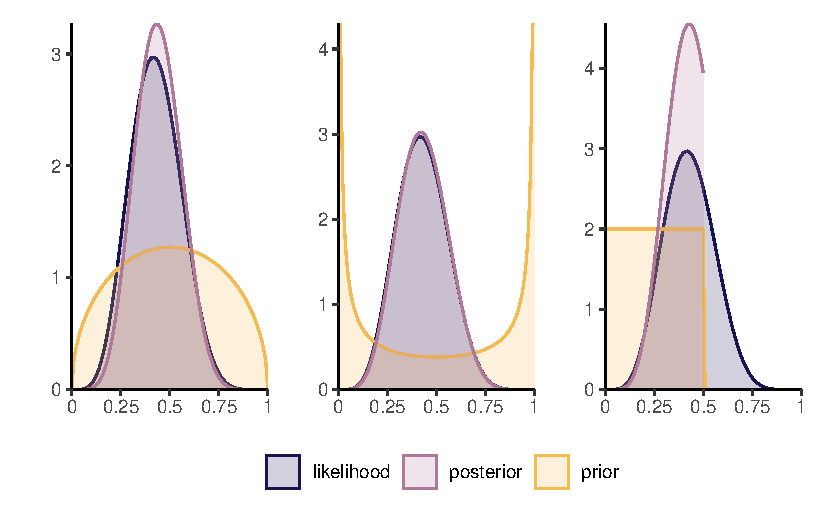
\includegraphics[keepaspectratio]{bayesics_files/figure-pdf/fig-betabinom-1.pdf}}

}

\caption{\label{fig-betabinom}Scaled binomial likelihood for six
successes out of 14 trials, with \(\mathsf{beta}(3/2, 3/2)\) prior
(left), \(\mathsf{beta}(1/4, 1/4)\) (middle) and truncated uniform on
\([0,1/2]\) (right), with the corresponding posterior distributions.}

\end{figure}%

\end{example}

\begin{remark}[Proportionality]
Any term appearing in the likelihood times prior function that does not
depend on parameters can be omitted since they will be absorbed by the
normalizing constant. This makes it useful to compute normalizing
constants or likelihood ratios.
\end{remark}

\begin{remark}
An alternative parametrization for the beta distribution sets
\(\alpha=\mu \kappa,\) \(\beta = (1-\mu)\kappa\) for \(\mu \in (0,1)\)
and \(\kappa>0,\) so that the model is parametrized directly in terms of
mean \(\mu,\) with \(\kappa\) capturing the dispersion.
\end{remark}

\begin{remark}
A density integrates to 1 over the range of possible outcomes, but there
is no guarantee that the likelihood function, as a function of
\(\boldsymbol{\theta},\) integrates to one over the parameter domain
\(\boldsymbol{\Theta}.\)

For example, the binomial likelihood with \(n\) trials and \(y\)
successes satisfies
\[\int_0^1 \binom{n}{y}\theta^y(1-\theta)^{n-y} \mathrm{d} \theta = \frac{1}{n+1}.\]

Moreover, the binomial distribution is discrete with support
\(0, \ldots, n,\) whereas the likelihood is continuous as a function of
the probability of success, as evidenced by
Figure~\ref{fig-binom-massvslik}

\begin{figure}[ht!]

\centering{

\pandocbounded{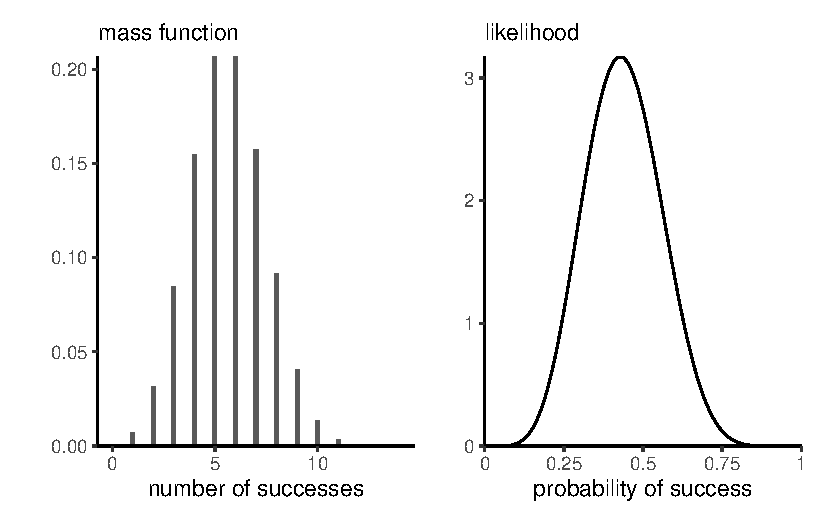
\includegraphics[keepaspectratio]{bayesics_files/figure-pdf/fig-binom-massvslik-1.pdf}}

}

\caption{\label{fig-binom-massvslik}Binomial mass function (left) and
scaled likelihood function (right).}

\end{figure}%

\end{remark}

\begin{definition}[Bayes factor and model
comparison]\protect\hypertarget{def-bayes-factor}{}\label{def-bayes-factor}

The marginal likelihood enters in the comparison of different models.
Suppose that we have models \(\mathcal{M}_m\) \((m=1, \ldots, M)\) to be
compared, with parameter vectors \(\boldsymbol{\theta}^{(m)}\) and data
vector \(\boldsymbol{y}.\) Consider \(p_m =\Pr(\mathcal{M}_m)\) the
prior probability of the different models under consideration, with
\(p_1 + \cdots + p_M = 1.\) The posterior odds for Models
\(\mathcal{M}_i\) vs \(\mathcal{M}_j\) are \begin{align*}
\underbracket[0.25pt]{\frac{\Pr(\mathcal{M}_i \mid \boldsymbol{y})}{\Pr(\mathcal{M}_j \mid \boldsymbol{y})}}_{\text{posterior odds}} = \underbracket[0.25pt]{\frac{p(\boldsymbol{y} \mid \mathcal{M}_i)}{p(\boldsymbol{y} \mid \mathcal{M}_j)}}_{\text{Bayes factor}} \underbracket[0.25pt]{\frac{\Pr(\mathcal{M}_i)}{\Pr(\mathcal{M}_j)}}_{\text{prior odds}}
\end{align*} where the first term on the right hand side is the Bayes
factor for model \(i\) vs \(j,\) denoted \(\mathsf{BF}_{ij}.\) The Bayes
factor is the ratio of marginal likelihoods, as \begin{align*}
p(\boldsymbol{y} \mid \mathcal{M}_i) = \int p(y \mid \boldsymbol{\theta}^{(i)}, \mathcal{M}_i) p( \boldsymbol{\theta}^{(i)} \mid \mathcal{M}_i) \mathrm{d}  \boldsymbol{\theta}^{(i)}.
\end{align*} Values of \(\mathsf{BF}_{ij}>1\) correspond to model
\(\mathcal{M}_i\) being more likely than \(\mathcal{M}_j.\)

While Bayes factors are used for model comparison, the answers depend
very strongly on the prior
\(p( \boldsymbol{\theta}^{(i)} \mid \mathcal{M}_i)\) specified and the
latter must be proper as a general rule for the ratio to be
well-defined.

The Bayes factor require that we compare the same data, but both
likelihood and priors could be different from one model to the next.

\end{definition}

\begin{example}[Bayes factor for the binomial
model]\protect\hypertarget{exm-bayesfactor}{}\label{exm-bayesfactor}

The marginal likelihood for the \(Y \mid P=p \sim \mathsf{binom}(n,p)\)
model with prior \(P \sim \mathsf{beta}(\alpha, \beta)\) is
\begin{align*}
p_{Y}(y) = \binom{n}{y} \frac{\mathrm{beta}(\alpha + y, \beta + n - y)}{\mathrm{beta}(\alpha, \beta)}.
\end{align*} where
\(\mathrm{beta}(\alpha, \beta) = \Gamma(\alpha)\Gamma(\beta)/\Gamma(\alpha+\beta)\)
is the beta function, expressed in terms of gamma functions.

Consider three models with
\(Y \mid P^{(i)}=p, \mathcal{M}_i \sim \mathsf{binom}(n, p)\) for
\(i=1, 2, 3\) and uniform, point mass and beta priors
\(P^{(1)}\sim \mathsf{unif}(0,1),\)
\(P^{(2)} \sim \mathsf{beta}(3/2, 3/2)\) and
\(P^{(3)}\sim \mathsf{1}_{p=0.5}.\) For \(\mathcal{M}_3,\) the marginal
likelihood is simply equal to the binomial distribution with \(p=0.5.\)

If \(n=14,\) but we let instead the number of success varies, the models
that put more mass closer to the ratio \(y/n\) will be favored. The
uniform prior in model \(\mathcal{M}_1\) will have a higher Bayes factor
than model \(\mathcal{M}_2\) or \(\mathcal{M}_3\) for values closer to
\(p=0\) or \(p=1,\) but there is mild evidence as shown in
Figure~\ref{fig-bayesfactor}.

\begin{Shaded}
\begin{Highlighting}[]
\CommentTok{\# Log of marginal posterior for binom with beta prior (default is uniform)}
\NormalTok{log\_marg\_post\_beta }\OtherTok{\textless{}{-}} \ControlFlowTok{function}\NormalTok{(n, y, }\AttributeTok{alpha =} \DecValTok{1}\NormalTok{, }\AttributeTok{beta =} \DecValTok{1}\NormalTok{)\{}
  \FunctionTok{lchoose}\NormalTok{(n, y) }\SpecialCharTok{+} \FunctionTok{lbeta}\NormalTok{(alpha }\SpecialCharTok{+}\NormalTok{ y, beta }\SpecialCharTok{+}\NormalTok{ n }\SpecialCharTok{{-}}\NormalTok{ y) }\SpecialCharTok{{-}} \FunctionTok{lbeta}\NormalTok{(alpha, beta)}
\NormalTok{\}}
\CommentTok{\# Log of Bayes factor}
\NormalTok{logBF2vs3 }\OtherTok{\textless{}{-}} \ControlFlowTok{function}\NormalTok{(y, n)\{ }\CommentTok{\# model 2 (beta(1.5,1.5) vs 3 (point mass at 0.5)}
  \FunctionTok{log\_marg\_post\_beta}\NormalTok{(}\AttributeTok{n =}\NormalTok{ n, }\AttributeTok{y =}\NormalTok{ y, }\AttributeTok{alpha =} \FloatTok{1.5}\NormalTok{, }\AttributeTok{beta =} \FloatTok{1.5}\NormalTok{) }\SpecialCharTok{{-}} \FunctionTok{dbinom}\NormalTok{(}\AttributeTok{x =}\NormalTok{ y, }\AttributeTok{size =}\NormalTok{ n, }\AttributeTok{prob =} \FloatTok{0.5}\NormalTok{, }\AttributeTok{log =} \ConstantTok{TRUE}\NormalTok{)}
\NormalTok{\}}
\end{Highlighting}
\end{Shaded}

\begin{figure}[ht!]

\centering{

\pandocbounded{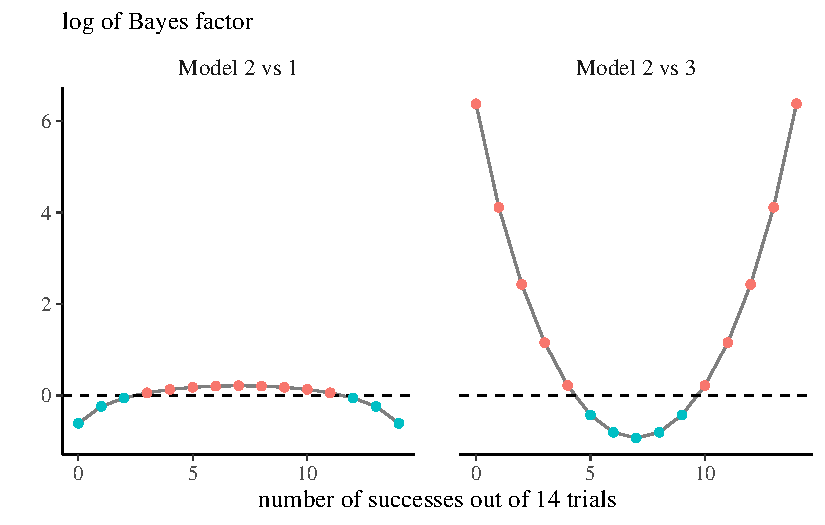
\includegraphics[keepaspectratio]{bayesics_files/figure-pdf/fig-bayesfactor-1.pdf}}

}

\caption{\label{fig-bayesfactor}Log of Bayes factors for comparison of
binomial models with \(n=14\) trials as a function of the number of
successes \(n.\) Values larger than zero (on log scale) indicate
preference for Model 2.}

\end{figure}%

\end{example}

\begin{proposition}[Sequentiality and Bayesian
updating]\protect\hypertarget{prp-sequentiality}{}\label{prp-sequentiality}

The likelihood is invariant to the order of the observations if they are
independent. Thus, if we consider two blocks of observations
\(\boldsymbol{y}_1\) and \(\boldsymbol{y}_2\)
\[p(\boldsymbol{\theta} \mid \boldsymbol{y}_1, \boldsymbol{y}_2) = p(\boldsymbol{\theta} \mid \boldsymbol{y}_1) p(\boldsymbol{\theta} \mid \boldsymbol{y}_2),\]
so it makes no difference if we treat data all at once or in blocks.
More generally, for data exhibiting spatial or serial dependence, it
makes sense to consider rather the conditional (sequential)
decomposition
\[f(\boldsymbol{y}; \boldsymbol{\theta}) = f(\boldsymbol{y}_1; \boldsymbol{\theta}) f(\boldsymbol{y}_2; \boldsymbol{\theta}, \boldsymbol{y}_1) \cdots f(\boldsymbol{y}_n; \boldsymbol{\theta}, \boldsymbol{y}_1, \ldots, \boldsymbol{y}_{n-1})\]
where
\(f(\boldsymbol{y}_k; \boldsymbol{y}_1, \ldots, \boldsymbol{y}_{k-1})\)
denotes the conditional density function given observations
\(\boldsymbol{y}_1, \ldots, \boldsymbol{y}_{k-1}.\)

By Bayes' rule, we can consider \emph{updating} the posterior by adding
terms to the likelihood, noting that \begin{align*}
p(\boldsymbol{\theta} \mid \boldsymbol{y}_1, \boldsymbol{y}_2) \propto p(\boldsymbol{y}_2 \mid \boldsymbol{y}_1, \boldsymbol{\theta}) p(\boldsymbol{\theta} \mid \boldsymbol{y}_1)
\end{align*} which amounts to treating the posterior
\(p(\boldsymbol{\theta} \mid \boldsymbol{y}_1)\) as a prior. If data are
exchangeable, the order in which observations are collected and the
order of the belief updating is irrelevant to the full posterior.
Figure~\ref{fig-sequential} shows how the posterior becomes gradually
closer to the scaled likelihood as we increase the sample size, and the
posterior mode moves towards the true value of the parameter (here 0.3).

\begin{figure}[ht!]

\centering{

\pandocbounded{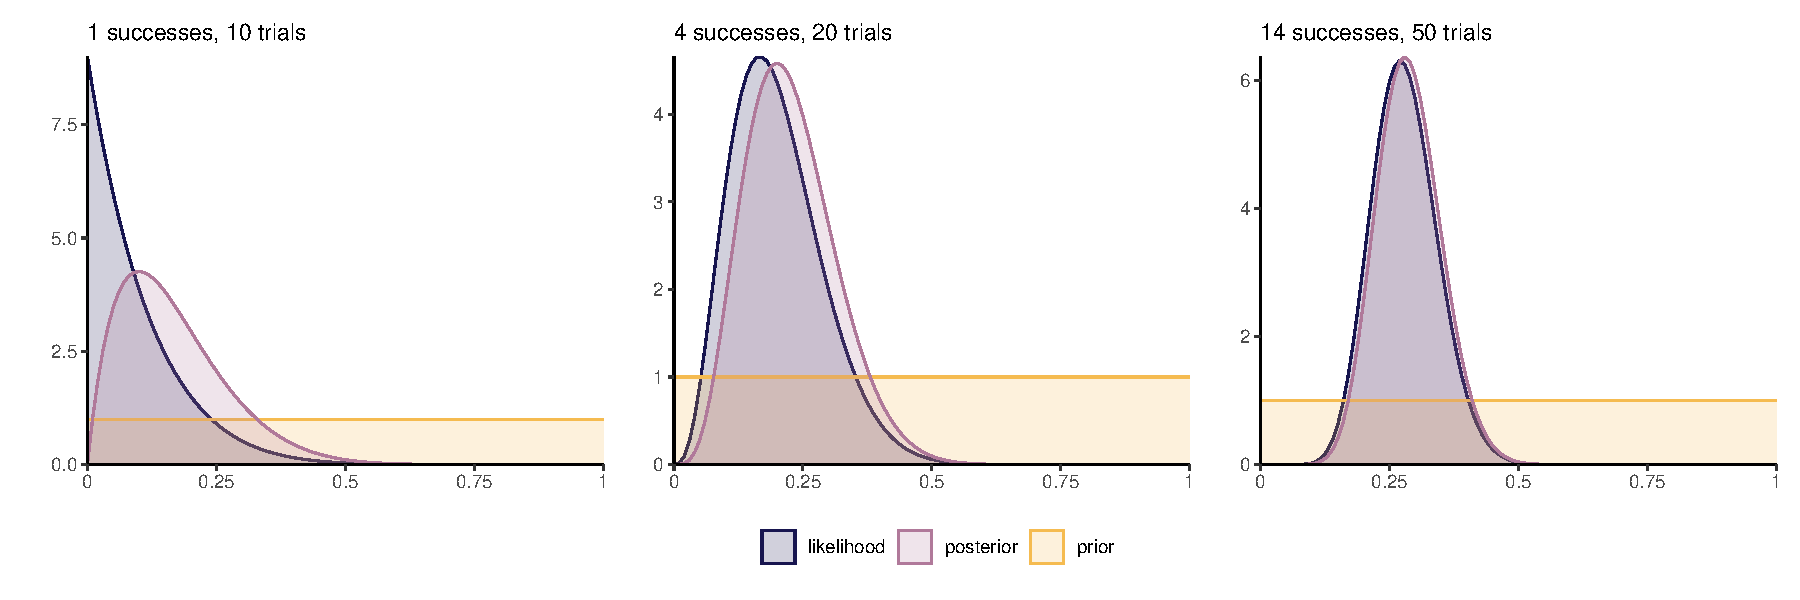
\includegraphics[keepaspectratio]{bayesics_files/figure-pdf/fig-sequential-1.pdf}}

}

\caption{\label{fig-sequential}Beta posterior and binomial likelihood
with a uniform prior for increasing number of observations (from left to
right) out of a total of 100 trials.}

\end{figure}%

\end{proposition}

\begin{example}[Numerical
integration]\protect\hypertarget{exm-numericalintegration}{}\label{exm-numericalintegration}

While we can calculate analytically the value of the normalizing
constant for the beta-binomial model, we could also for arbitrary priors
use numerical integration or Monte Carlo methods in the event the
parameter vector \(\boldsymbol{\theta}\) is low-dimensional.

While estimation of the normalizing constant is possible in simple
models, the following highlights some challenges that are worth keeping
in mind. In a model for discrete data (that is, assigning probability
mass to a countable set of outcomes), the terms in the likelihood are
probabilities and thus the likelihood becomes smaller as we gather more
observations (since we multiply terms between zero or one). The marginal
likelihood term becomes smaller and smaller, so it's reciprocal is big
and this can lead to arithmetic underflow.

\begin{Shaded}
\begin{Highlighting}[]
\NormalTok{y }\OtherTok{\textless{}{-}} \DecValTok{6}\NormalTok{L }\CommentTok{\# number of successes }
\NormalTok{n }\OtherTok{\textless{}{-}} \DecValTok{14}\NormalTok{L }\CommentTok{\# number of trials}
\NormalTok{alpha }\OtherTok{\textless{}{-}}\NormalTok{ beta }\OtherTok{\textless{}{-}} \FloatTok{1.5} \CommentTok{\# prior parameters}
\NormalTok{unnormalized\_posterior }\OtherTok{\textless{}{-}} \ControlFlowTok{function}\NormalTok{(theta)\{}
\NormalTok{  theta}\SpecialCharTok{\^{}}\NormalTok{(y}\SpecialCharTok{+}\NormalTok{alpha}\DecValTok{{-}1}\NormalTok{) }\SpecialCharTok{*}\NormalTok{ (}\DecValTok{1}\SpecialCharTok{{-}}\NormalTok{theta)}\SpecialCharTok{\^{}}\NormalTok{(n}\SpecialCharTok{{-}}\NormalTok{y }\SpecialCharTok{+}\NormalTok{ beta }\SpecialCharTok{{-}} \DecValTok{1}\NormalTok{)}
\NormalTok{\}}
\FunctionTok{integrate}\NormalTok{(}\AttributeTok{f =}\NormalTok{ unnormalized\_posterior,}
          \AttributeTok{lower =} \DecValTok{0}\NormalTok{,}
          \AttributeTok{upper =} \DecValTok{1}\NormalTok{)}
\end{Highlighting}
\end{Shaded}

\begin{verbatim}
1.066906e-05 with absolute error < 1e-12
\end{verbatim}

\begin{Shaded}
\begin{Highlighting}[]
\CommentTok{\# Compare with known constant}
\FunctionTok{beta}\NormalTok{(y }\SpecialCharTok{+}\NormalTok{ alpha, n }\SpecialCharTok{{-}}\NormalTok{ y }\SpecialCharTok{+}\NormalTok{ beta)}
\end{Highlighting}
\end{Shaded}

\begin{verbatim}
[1] 1.066906e-05
\end{verbatim}

\begin{Shaded}
\begin{Highlighting}[]
\CommentTok{\# Monte Carlo integration}
\FunctionTok{mean}\NormalTok{(}\FunctionTok{unnormalized\_posterior}\NormalTok{(}\FunctionTok{runif}\NormalTok{(}\FloatTok{1e5}\NormalTok{)))}
\end{Highlighting}
\end{Shaded}

\begin{verbatim}
[1] 1.064067e-05
\end{verbatim}

\end{example}

When \(\boldsymbol{\theta}\) is high-dimensional, the marginal
likelihood is intractable. This is one of the main challenges of
Bayesian statistics and the popularity and applicability has grown
drastically with the development and popularity of numerical algorithms,
following the publication of Geman and Geman
(\citeproc{ref-Geman.Geman:1984}{1984}) and Gelfand and Smith
(\citeproc{ref-Gelfand.Smith:1990}{1990}). Markov chain Monte Carlo
methods circumvent the calculation of the denominator by drawing
approximate samples from the posterior.

\begin{example}[Importance of selling
format]\protect\hypertarget{exm-Duke-Amir}{}\label{exm-Duke-Amir}

Duke and Amir (\citeproc{ref-Duke.Amir:2023}{2023}) consider the
difference between integrated and sequential format for sales. The
\texttt{sellingformat} dataset contains \(n=397\) observations split
into two groups: quantity-integrated decision (decide the amount to buy)
and quantity-sequential (first select buy, then select the amount).
Participants of the study were randomly allocated to either of these two
format and their decision, either buy, \texttt{1}, or do not buy
\texttt{0}, is recorded.

\begin{longtable}[]{@{}lrr@{}}

\caption{\label{tbl-contingency-sellingformat}Aggregated data from Duke
and Amir (2023), experiment 1. Number of participants who did not
(\texttt{0}) or did buy (\texttt{1}) products as a function of
experimental condition.}

\tabularnewline

\toprule\noalign{}
& 0 & 1 \\
\midrule\noalign{}
\endhead
\bottomrule\noalign{}
\endlastfoot
quantity-integrated & 152 & 46 \\
quantity-sequential & 176 & 23 \\

\end{longtable}

We consider the number of purchased out of the total, treating records
as independent Bernoulli observations with a flat (uniform prior).

With a beta-binomial model, the posterior for the probability of buying
is \(\mathsf{beta}(47, 153)\) for quantity-integrated and
\(\mathsf{beta}(24, 177)\) for quantity-sequential. We can compute the
posterior of the odds ratio,
\[O = \frac{\Pr(Y=1 \mid \texttt{integrated})}{\Pr(Y=0 \mid \texttt{integrated})}\frac{\Pr(Y=0 \mid \texttt{sequential})}{\Pr(Y=1 \mid \texttt{sequential})},\]
by simulating independent draws from the posteriors of each condition
and computing the odds ratio.

\begin{Shaded}
\begin{Highlighting}[]
\FunctionTok{data}\NormalTok{(sellingformat, }\AttributeTok{package =} \StringTok{"hecbayes"}\NormalTok{)}
\NormalTok{contingency }\OtherTok{\textless{}{-}} \FunctionTok{with}\NormalTok{(sellingformat, }\FunctionTok{table}\NormalTok{(format, purchased))}
\CommentTok{\# Posterior draws of the parameters}
\NormalTok{post\_p\_int }\OtherTok{\textless{}{-}} \FunctionTok{rbeta}\NormalTok{(}\AttributeTok{n =} \FloatTok{1e4}\NormalTok{, }\AttributeTok{shape1 =} \DecValTok{47}\NormalTok{, }\AttributeTok{shape2 =} \DecValTok{153}\NormalTok{)}
\NormalTok{post\_p\_seq }\OtherTok{\textless{}{-}} \FunctionTok{rbeta}\NormalTok{(}\AttributeTok{n =} \FloatTok{1e4}\NormalTok{, }\AttributeTok{shape1 =} \DecValTok{24}\NormalTok{, }\AttributeTok{shape2 =} \DecValTok{177}\NormalTok{)}
\CommentTok{\# Reparametrization}
\NormalTok{post\_odds\_int }\OtherTok{\textless{}{-}}\NormalTok{ (post\_p\_int }\SpecialCharTok{/}\NormalTok{ (}\DecValTok{1} \SpecialCharTok{{-}}\NormalTok{ post\_p\_int))}
\NormalTok{post\_odds\_seq }\OtherTok{\textless{}{-}}\NormalTok{ (post\_p\_seq }\SpecialCharTok{/}\NormalTok{ (}\DecValTok{1} \SpecialCharTok{{-}}\NormalTok{ post\_p\_seq))}
\NormalTok{post\_oddsratio }\OtherTok{\textless{}{-}}\NormalTok{ post\_odds\_int }\SpecialCharTok{/}\NormalTok{ post\_odds\_seq}
\end{Highlighting}
\end{Shaded}

Figure~\ref{fig-post-Duke_Amir} shows the posterior of the probability
of buying for each group, and the odds. It is clear that the integrated
format leads to much more sales in the experiment, with a posterior
ratio exceeding 1 with probability \(99.89\%.\)

\begin{figure}[ht!]

\centering{

\pandocbounded{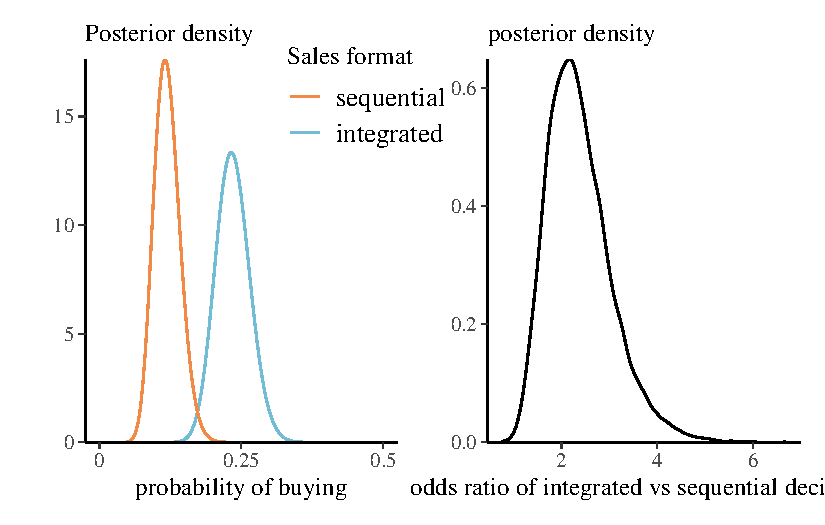
\includegraphics[keepaspectratio]{bayesics_files/figure-pdf/fig-post-Duke_Amir-1.pdf}}

}

\caption{\label{fig-post-Duke_Amir}Posterior curves per group (left) and
odds ratio (right)}

\end{figure}%

\end{example}

\section{Posterior predictive
distribution}\label{posterior-predictive-distribution}

Prediction in the Bayesian paradigm is obtained by considering the
\emph{posterior predictive distribution}, \begin{align*}
p(y_{\text{new}} \mid \boldsymbol{y}) =
\int_{\Theta} p(y_{\text{new}}  \mid \boldsymbol{\theta}) p(\boldsymbol{\theta} \mid  \boldsymbol{y}) \mathrm{d} \boldsymbol{\theta}
\end{align*}

Given draws from the posterior distribution, say
\(\boldsymbol{\theta}_b\) \((b=1, \ldots, B),\) we sample from each a
new realization from the distribution appearing in the likelihood
\(p(y_{\text{new}}  \mid \boldsymbol{\theta}_b).\) This is different
from the frequentist setting, which fixes the value of the parameter to
some estimate \(\widehat{\boldsymbol{\theta}}\); by contrast, the
posterior predictive, here a beta-binomial distribution
\(\mathsf{BetaBin}(n, \alpha + y, n - y + \beta),\) carries over the
uncertainty so will typically be wider and overdispersed relative to the
corresponding binomial model. This can be easily seen from the
left-panel of Figure~\ref{fig-betabinompostpred}, which contrasts the
binomial mass function evaluated at the maximum likelihood estimator
\(\widehat{\theta}=6/14\) with the posterior predictive.

\begin{Shaded}
\begin{Highlighting}[]
\NormalTok{npost }\OtherTok{\textless{}{-}} \FloatTok{1e4}\NormalTok{L}
\CommentTok{\# Sample draws from the posterior distribution}
\NormalTok{post\_samp }\OtherTok{\textless{}{-}} \FunctionTok{rbeta}\NormalTok{(}\AttributeTok{n =}\NormalTok{ npost, y }\SpecialCharTok{+}\NormalTok{ alpha, n }\SpecialCharTok{{-}}\NormalTok{ y }\SpecialCharTok{+}\NormalTok{ beta)}
\CommentTok{\# For each draw, sample new observation}
\NormalTok{post\_pred }\OtherTok{\textless{}{-}} \FunctionTok{rbinom}\NormalTok{(}\AttributeTok{n =}\NormalTok{ npost, }\AttributeTok{size =}\NormalTok{ n, }\AttributeTok{prob =}\NormalTok{ post\_samp)}
\end{Highlighting}
\end{Shaded}

\begin{figure}[ht!]

\centering{

\pandocbounded{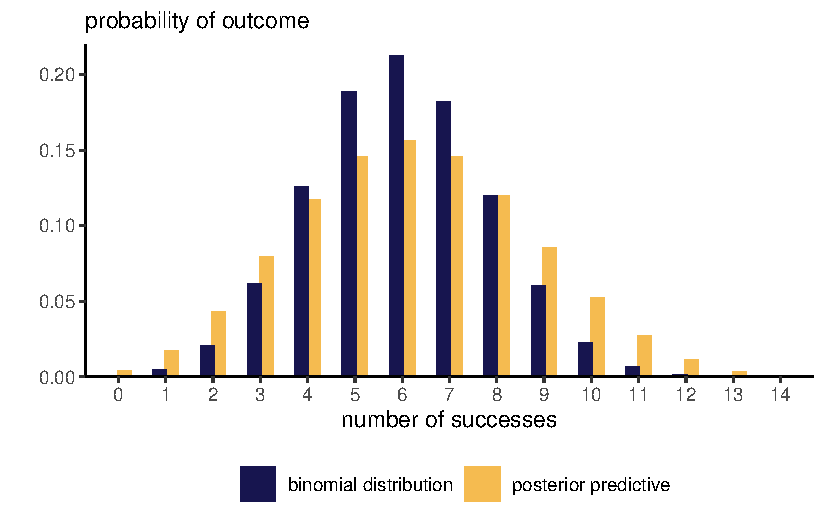
\includegraphics[keepaspectratio]{bayesics_files/figure-pdf/fig-betabinompostpred-1.pdf}}

}

\caption{\label{fig-betabinompostpred}Beta-binomial posterior predictive
distribution with corresponding binomial mass function evaluated at the
maximum likelihood estimator.}

\end{figure}%

Given the \(\mathsf{Be}(a, b)\) posterior with \(a=y + \alpha\) and
\(b=n-y + \beta,\) the predictive distribution of \(Y_{\text{new}}\) for
fixed \(n_{\text{new}}\) number of trials is beta-binomial with mass
function \begin{align*}
p(y_{\text{new}}\mid y) &= \int_0^1 \binom{n_{\text{new}}}{y_{\text{new}}} \frac{\theta^{a + y_{\text{new}}-1}(1-\theta)^{b + n_{\text{new}} - y_{\text{new}}-1}}{
\mathrm{Be}(a, b)}\mathrm{d} \theta
\\&= \binom{n_{\text{new}}}{y_{\text{new}}} \frac{\mathrm{Be}(a + y_{\text{new}}, b + n_{\text{new}} - y_{\text{new}})}{\mathrm{Be}(a, b)}
\end{align*}

\begin{example}[Posterior predictive distribution of univariate Gaussian
with known
mean]\protect\hypertarget{exm-normal-post-pred}{}\label{exm-normal-post-pred}

Consider an \(n\) sample of independent and identically distributed
Gaussian, \(Y_i \sim \mathsf{Gauss}(0, \tau^{-1})\)
(\(i=1, \ldots, n\)), where we assign a gamma prior on the precision
\(\tau \sim \mathsf{gamma}(\alpha, \beta).\) The posterior is
\begin{align*}
p(\tau \mid \boldsymbol{y}) \stackrel{\tau}{\propto} \prod_{i=1}^n \tau^{n/2}\exp\left(-\tau \frac{\sum_{i=1}^n{y_i^2}}{2}\right) \times \tau^{\alpha-1} \exp(-\beta \tau)
\end{align*} and rearranging the terms to collect powers of \(\tau,\)
etc. we find that the posterior for \(\tau\) must also be gamma, with
shape parameter \(\alpha^* = \alpha + n/2\) and rate
\(\beta^* = \beta + \sum_{i=1}^n y_i^2/2.\)

The posterior predictive is \begin{align*}
p(y_{\text{new}} \mid \boldsymbol{y}) &= \int_0^\infty \frac{\tau^{1/2}}{(2\pi)^{1/2}}\exp(-\tau y_{\text{new}}^2/2) \frac{\beta^{*\alpha^*}}{\Gamma(\alpha^*)}\tau^{\alpha^*-1}\exp(-\beta^* \tau) \mathrm{d} \tau 
\\&= (2\pi)^{-1/2} \frac{\beta^{*\alpha^*}}{\Gamma(\alpha^*)} \int_0^\infty\tau^{\alpha^*-1/2} \exp\left\{- \tau (y_{\text{new}}^2/2 + \beta^*)\right\} \mathrm{d} \tau
\\&= (2\pi)^{-1/2} \frac{\beta^{*\alpha^*}}{\Gamma(\alpha^*)} \frac{\Gamma(\alpha^* + 1/2)}{(y_{\text{new}}^2/2 + \beta^*)^{\alpha^*+1/2}}
\\&= \frac{\Gamma\left(\frac{2\alpha^* + 1}{2}\right)}{\sqrt{2\pi}\Gamma\left(\frac{2\alpha^*}{2}\right)\beta^{*1/2}} \left( 1+ \frac{y_{\text{new}}^2}{2\beta^*}\right)^{-\alpha^*-1/2}
\\&= \frac{\Gamma\left(\frac{2\alpha^* + 1}{2}\right)}{\sqrt{\pi}\sqrt{ 2\alpha^*}\Gamma\left(\frac{2\alpha^*}{2}\right)(\beta^*/\alpha^*)^{1/2}} \left( 1+ \frac{1}{2\alpha^*}\frac{y_{\text{new}}^2}{(\beta^*/\alpha^*)}\right)^{-\alpha^*-1/2}
\end{align*} which entails that \(Y_{\text{new}}\) is a scaled
Student-\(t\) distribution with scale \((\beta^*/\alpha^*)^{1/2}\) and
\(2\alpha+n\) degrees of freedom. This example also exemplifies the
additional variability relative to the distribution generating the data:
indeed, the Student-\(t\) distribution is more heavy-tailed than the
Gaussian, but since the degrees of freedom increase linearly with \(n,\)
the distribution converges to a Gaussian as \(n \to \infty,\) reflecting
the added information as we collect more and more data points and the
variance gets better estimated through \(\sum_{i=1}^n y_i^2/n.\)

\end{example}

\section{Summarizing posterior
distributions}\label{summarizing-posterior-distributions}

The output of the Bayesian learning problem will be either of:

\begin{enumerate}
\def\labelenumi{\arabic{enumi}.}
\tightlist
\item
  a fully characterized distribution
\item
  a numerical approximation to the posterior distribution (pointwise)
\item
  an exact or approximate sample drawn from the posterior distribution
\end{enumerate}

In the first case, we will be able to directly evaluate quantities of
interest if there are closed-form expressions for the latter, or else we
could draw samples from the distribution and evaluate them via
Monte-Carlo. In case of numerical approximations, we will need to resort
to numerical integration or otherwise to get our answers.

Often, we will also be interested in the marginal posterior distribution
of each component \(\theta_j\) in turn (\(j=1, \ldots, J\)). To get
these, we carry out additional integration steps,
\[p(\theta_j \mid \boldsymbol{y}) = \int p(\boldsymbol{\theta} \mid \boldsymbol{y}) \mathrm{d} \boldsymbol{\theta}_{-j}.\]
With a posterior sample, this is trivial: it suffices to keep the column
corresponding to \(\theta_j\) and discard the others.

Most of the field of Bayesian statistics revolves around the creation of
algorithms that either circumvent the calculation of the normalizing
constant (notably using Monte Carlo and Markov chain Monte Carlo
methods) or else provide accurate numerical approximation of the
posterior pointwise, including for marginalizing out all but one
parameters (integrated nested Laplace approximations, variational
inference, etc.) The target of inference is the whole posterior
distribution, a potentially high-dimensional object which may be
difficult to summarize or visualize. We can thus report only
characteristics of the the latter.

The choice of point summary to keep has it's root in decision theory.

\begin{definition}[Loss
function]\protect\hypertarget{def-lossfunction}{}\label{def-lossfunction}

A loss function \(c(\boldsymbol{\theta}, \boldsymbol{\upsilon})\) is a
mapping from \(\mathbb{R}^p \to \mathbb{R}^k\) that assigns a weight to
each value of \(\boldsymbol{\theta},\) corresponding to the regret or
loss arising from choosing this value. The corresponding point estimator
\(\widehat{\boldsymbol{\upsilon}}\) is the minimizer of the expected
loss,

\begin{align*}
\widehat{\boldsymbol{\upsilon}} &= \mathop{\mathrm{argmin}}_{\boldsymbol{\upsilon}}\mathsf{E}_{\boldsymbol{\Theta} \mid \boldsymbol{Y}}\{c(\boldsymbol{\theta}, \boldsymbol{v})\} \\&=\mathop{\mathrm{argmin}}_{\boldsymbol{\upsilon}} \int_{\mathbb{R}^d} c(\boldsymbol{\theta}, \boldsymbol{\upsilon})p(\boldsymbol{\theta} \mid \boldsymbol{y}) \mathrm{d} \boldsymbol{\theta}
\end{align*}

\end{definition}

For example, in a univariate setting, the quadratic loss
\(c(\theta, \upsilon) = (\theta-\upsilon)^2\) returns the posterior
mean, the absolute loss \(c(\theta, \upsilon)=|\theta - \upsilon|\)
returns the posterior median and the 0-1 loss
\(c(\theta, \upsilon) = \mathrm{I}(\upsilon \neq \theta)\) returns the
posterior mode.

For example consider the quadratic loss function which is
differentiable. Provided we can interchange differential operator and
integral sign, \begin{align*}
0&= \int_{\mathbb{R}} \frac{\partial (\upsilon-\theta)^2}{\partial \upsilon} p(\theta \mid \boldsymbol{y}) \mathrm{d} \theta 
\\&= \int_{\mathbb{R}} \frac{\partial 2(\upsilon-\theta)}{\partial \upsilon} p(\theta \mid \boldsymbol{y}) \mathrm{d} \theta 
\\& = 2\upsilon - 2 \mathsf{E}(\theta)
\end{align*} which is minimized when
\(\widehat{\upsilon}=\mathsf{E}_{\Theta \mid \boldsymbol{Y}}(\theta)\).

All of these point estimators are central tendency measures, but some
may be more adequate depending on the setting as they can correspond to
potentially different values, as shown in the left-panel of
Figure~\ref{fig-central-moments}. The choice is application specific:
for multimodal distributions, the mode is likely a better choice.

If we know how to evaluate the distribution numerically, we can optimize
to find the mode or else return the value for the pointwise evaluation
on a grid at which the density achieves it's maximum. The mean and
median would have to be evaluated by numerical integration if there is
no closed-form expression for the latter.

If we have rather a sample from the posterior with associated posterior
density values, then we can obtain the mode as the parameter combination
with the highest posterior, the median from the value at rank
\(\lfloor n/2\rfloor\) and the mean through the sample mean of posterior
draws.

\begin{figure}[ht!]

\centering{

\pandocbounded{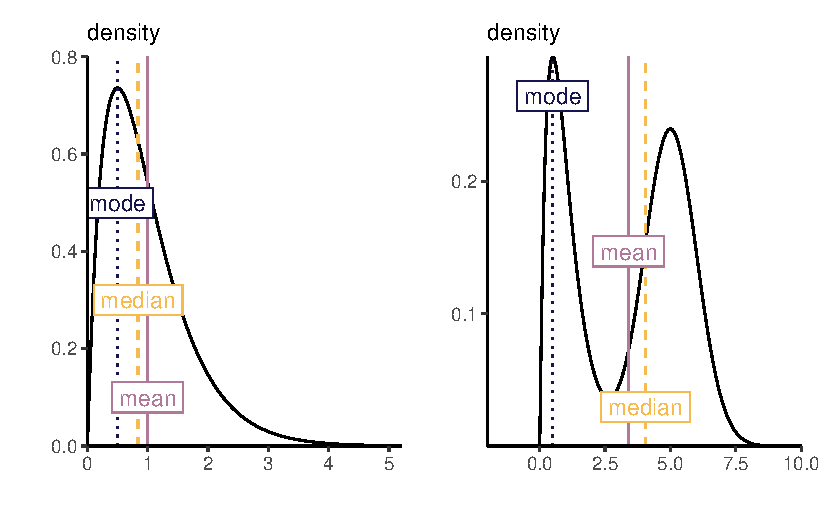
\includegraphics[keepaspectratio]{bayesics_files/figure-pdf/fig-central-moments-1.pdf}}

}

\caption{\label{fig-central-moments}Point estimators from a right-skewed
distribution (left) and from a multimodal distribution (right).}

\end{figure}%

The loss function is often a functional (meaning a one-dimensional
summary) from the posterior. The following example shows how it reduces
a three-dimensional problem into a single risk measure.

\begin{example}[Value-at-risk for Danish insurance
losses]\protect\hypertarget{exm-loss-extremes}{}\label{exm-loss-extremes}

In extreme value, we are often interested in assessing the risk of
events that are rare enough that they lie beyond the range of observed
data. To provide a scientific extrapolation, it often is justified to
fit a generalized Pareto distribution to exceedances of \(Z=Y-u,\) for
some user-specified threshold \(u\) which is often taken as a large
quantile of the distribution of
\(Z \sim \mathsf{gen. Pareto}(\tau, \xi);\) see
Definition~\ref{def-gen-pareto}

Insurance companies provide coverage in exchange for premiums, but need
to safeguard themselves against very high claims by buying reinsurance
products. These risks are often communicated through the value-at-risk
(VaR), a high quantile exceeded with probability \(p.\) We model Danish
fire insurance claim amounts for inflation-adjusted data collected from
January 1980 until December 1990 that are in excess of a million Danish
kroner, found in the \texttt{evir} package and analyzed in Example 7.23
of McNeil, Frey, and Embrechts
(\citeproc{ref-McNeil.Frey.Embrechts:2005}{2005}). These claims are
denoted \(Y\) and there are 2167 observations.

We fit a generalized Pareto distribution to exceedances above 10
millions krones, keeping 109 observations or roughly the largest 5\% of
the original sample. Preliminary analysis shows that we can treat data
as roughly independent and identically distributed and goodness-of-fit
diagnostics (not shown) for the generalized Pareto suggest that the fit
is adequate for all but the three largest observations, which are
(somewhat severely) underestimated by the model.

\begin{figure}[ht!]

\centering{

\pandocbounded{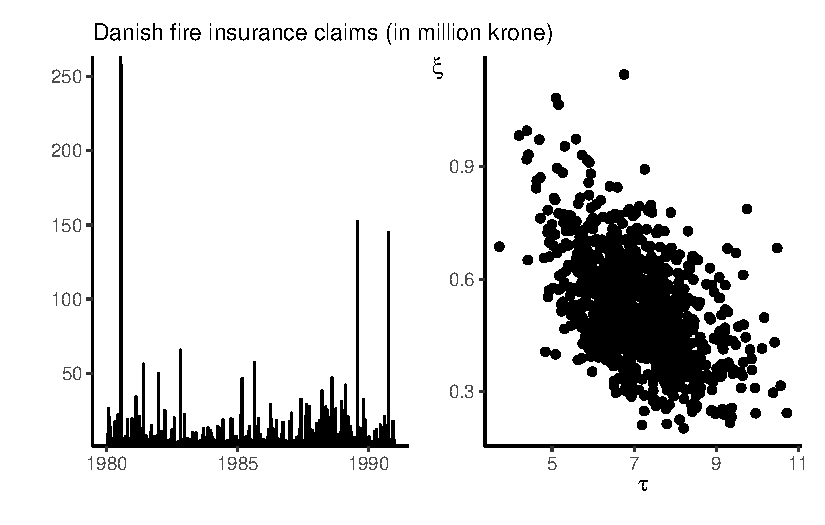
\includegraphics[keepaspectratio]{bayesics_files/figure-pdf/fig-danish-1.pdf}}

}

\caption{\label{fig-danish}Time series of Danish fire claims exceeding a
million krone (left) and posterior samples from the scale \(\tau\) and
shape \(\xi\) of the generalized Pareto model fitted to exceedances
above 10 million krone (right).}

\end{figure}%

The generalized Pareto model only describes the \(n_u\) exceedances
above \(u=10,\) so we need to incorporate in the likelihood a binomial
contribution for the probability \(\zeta_u\) of exceeding the threshold
\(u.\) The log likelihood for the full model for \(y_i>u\) is
\begin{align*}
\ell(\tau, \xi, \zeta_u) &\propto -109 \log \tau + \sum_{i=1}^{109} (1+1/\xi)\log\left(1+\xi\frac{y_i-10}{\tau}\right)_{+} + \\& \quad   109\log \zeta_u + 2058 \log(1-\zeta_u), 
\end{align*} Provided that the priors for \((\tau, \xi)\) are
independent of those for \(\zeta_u,\) the posterior also factorizes as a
product, so \(\zeta_u\) and \((\tau, \xi)\) are a posteriori
independent.

Suppose for now that we set a \(\mathsf{beta}(0.5, 0.5)\) prior for
\(\zeta_u\) and a non-informative prior for the generalized Pareto
parameters.

We consider the modelling of insurance losses exceeding \(u=10\)
millions krones using a generalized Pareto distribution to the
\texttt{danish} fire insurance data with some prior; see
Definition~\ref{def-gen-pareto} for the model. The model has three
parameters: the scale \(\tau\), the shape \(\xi\) and the probability of
exceeding the threshold \(\zeta_u\).

Our aim is to evaluate the posterior distribution for the value-at-risk,
the \(\alpha\) quantile of \(Y\) for high values of \(\alpha\) and see
what point estimator one would obtain depending on our choice of loss
function. For any \(\alpha > 1-\zeta_u,\) the \(q_{\alpha}\) can be
written in terms of the generalized Pareto survival function times the
probability of exceedance above the threshold, \begin{align*}
1- \alpha  &= \Pr(Y > q_\alpha \mid Y > u) \Pr(Y > u) 
\\ &= \left(1+\xi \frac{q_{\alpha}-u}{\tau}\right)_{+}^{-1/\xi}\zeta_u
\end{align*} and solving for \(q_{\alpha}\) gives \begin{align*}
q_{\alpha} = u+ \frac{\tau}{\xi} \left\{\left(\frac{\zeta_u}{1-\alpha}\right)^\xi-1\right\}.
\end{align*} We obtained, using tools that will be discussed in
Example~\ref{exm-rust}, a matrix \texttt{post\_samp} that contains exact
samples from the posterior distribution of \((\tau, \xi, \zeta_u).\) To
obtain the posterior distribution of the \(\alpha\) quantile,
\(q_{\alpha},\) it thus suffices to plug in each posterior sample and
evaluate the function: the uncertainty is carried over from the
simulated values of the parameters to those of the quantile
\(q_{\alpha}.\) The left panel of Figure~\ref{fig-lossfn} shows the
posterior density estimate of the \(\mathsf{VaR}(0.99)\) along with the
maximum a posteriori (mode) of the latter.

Suppose that we prefer to under-estimate the value-at-risk rather than
overestimate: this could be captured by the custom loss function
\begin{align*}
c(q, q_0) = 
\begin{cases}
0.5(0.99q - q_0), & q > q_0 \\
0.75(q_0 - 1.01q), & q < q_0.
\end{cases}
\end{align*} For a given value of the value-at-risk \(q_0\) evaluated on
a grid, we thus compute \begin{align*}
 r(q_0) = \int_{\boldsymbol{\Theta}}c(q(\boldsymbol{\theta}), q_0) p (\boldsymbol{\theta} \mid \boldsymbol{y}) \mathrm{d} \boldsymbol{\theta}
\end{align*} and we seek to minimize the risk,
\(\widehat{q} =\mathrm{argmin}_{q_0 \in \mathbb{R}_{+}} r(q_0).\) The
value returned that minimizes the loss, shown in
Figure~\ref{fig-lossfn}, is to the left of the posterior mean for
\(q_\alpha.\)

\begin{Shaded}
\begin{Highlighting}[]
\CommentTok{\# Compute value at risk from generalized Pareto distribution quantile fn}
\NormalTok{VaR\_post }\OtherTok{\textless{}{-}} \FunctionTok{with}\NormalTok{(post\_samp,   }\CommentTok{\# data frame of posterior draws}
\NormalTok{            revdbayes}\SpecialCharTok{::}\FunctionTok{qgp}\NormalTok{(   }\CommentTok{\# with columns \textquotesingle{}probexc\textquotesingle{}, \textquotesingle{}scale\textquotesingle{}, \textquotesingle{}shape\textquotesingle{}}
  \AttributeTok{p =} \FloatTok{0.01}\SpecialCharTok{/}\NormalTok{probexc, }
  \AttributeTok{loc =} \DecValTok{10}\NormalTok{, }
  \AttributeTok{scale =}\NormalTok{ scale, }
  \AttributeTok{shape =}\NormalTok{ shape, }
  \AttributeTok{lower.tail =} \ConstantTok{FALSE}\NormalTok{))}
\CommentTok{\# Loss function}
\NormalTok{loss }\OtherTok{\textless{}{-}} \ControlFlowTok{function}\NormalTok{(qhat, q)\{}
    \FunctionTok{mean}\NormalTok{(}\FunctionTok{ifelse}\NormalTok{(q }\SpecialCharTok{\textgreater{}}\NormalTok{ qhat,}
           \FloatTok{0.5}\SpecialCharTok{*}\NormalTok{(}\FloatTok{0.99}\SpecialCharTok{*}\NormalTok{q}\SpecialCharTok{{-}}\NormalTok{qhat),}
           \FloatTok{0.75}\SpecialCharTok{*}\NormalTok{(qhat}\FloatTok{{-}1.01}\SpecialCharTok{*}\NormalTok{q)))}
\NormalTok{\}}
\CommentTok{\# Create a grid of values over which to estimate the loss for VaR}
\NormalTok{nvals }\OtherTok{\textless{}{-}} \DecValTok{101}\NormalTok{L}
\NormalTok{VaR\_grid }\OtherTok{\textless{}{-}} \FunctionTok{seq}\NormalTok{(}
  \AttributeTok{from =} \FunctionTok{quantile}\NormalTok{(VaR\_post, }\FloatTok{0.01}\NormalTok{),}
  \AttributeTok{to =} \FunctionTok{quantile}\NormalTok{(VaR\_post, }\FloatTok{0.99}\NormalTok{), }
  \AttributeTok{length.out =}\NormalTok{ nvals)}
\CommentTok{\# Create a container to store results}
\NormalTok{risk }\OtherTok{\textless{}{-}} \FunctionTok{numeric}\NormalTok{(}\AttributeTok{length =}\NormalTok{ nvals)}
\ControlFlowTok{for}\NormalTok{(i }\ControlFlowTok{in} \FunctionTok{seq\_len}\NormalTok{(nvals))\{}
  \CommentTok{\# Compute integral (Monte Carlo average over draws)}
\NormalTok{ risk[i] }\OtherTok{\textless{}{-}} \FunctionTok{loss}\NormalTok{(}\AttributeTok{q =}\NormalTok{ VaR\_post, }\AttributeTok{qhat =}\NormalTok{ VaR\_grid[i])}
\NormalTok{\}}
\end{Highlighting}
\end{Shaded}

\begin{figure}[ht!]

\centering{

\pandocbounded{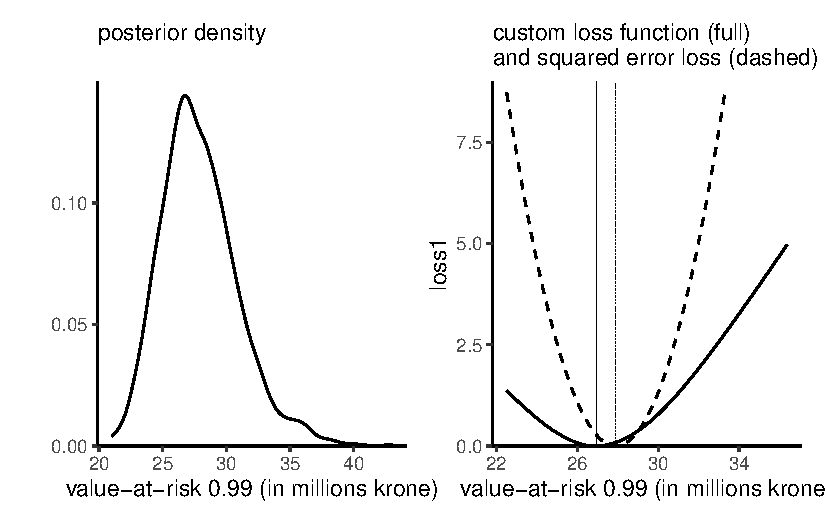
\includegraphics[keepaspectratio]{bayesics_files/figure-pdf/fig-lossfn-1.pdf}}

}

\caption{\label{fig-lossfn}Posterior density (left) and losses functions
for the 0.99 value-at-risk for the Danish fire insurance data. The
vertical lines denote point estimates of the quantiles that minimize the
loss functions.}

\end{figure}%

\end{example}

To communicate uncertainty, we may resort to credible regions and
intervals.

\begin{definition}[]\protect\hypertarget{def-credible-region}{}\label{def-credible-region}

A \((1-\alpha)\) \textbf{credible region} (or credible interval in the
univariate setting) is a set \(\mathcal{S}_\alpha\) such that, with
probability level \(\alpha,\) \begin{align*}
\Pr(\boldsymbol{\theta} \in \mathcal{S}_\alpha \mid \boldsymbol{Y}=\boldsymbol{y}) = 1-\alpha
\end{align*}

\end{definition}

These intervals are not unique, as are confidence sets. In the
univariate setting, the central or equitailed interval are the most
popular, and easily obtained by considering the \(\alpha/2, 1-\alpha/2\)
quantiles. These are easily obtained from samples by simply taking
empirical quantiles. An alternative, highest posterior density credible
sets, which may be a set of disjoint intervals obtained by considering
the parts of the posterior with the highest density, may be more
informative. The top panel Figure~\ref{fig-credible-intervals} shows two
extreme cases in which these intervals differ: the distinction for a
bimodal mixture distribution, and a even more striking difference for
50\% credible intervals for a symmetric beta distribution whose mass lie
near the endpoints of the distribution, leading to no overlap between
the two intervals.

\begin{Shaded}
\begin{Highlighting}[]
\FunctionTok{set.seed}\NormalTok{(}\DecValTok{2023}\NormalTok{)}
\NormalTok{postsamp }\OtherTok{\textless{}{-}} \FunctionTok{rbeta}\NormalTok{(}\AttributeTok{n =} \DecValTok{1000}\NormalTok{, }\AttributeTok{shape1 =} \FloatTok{0.5}\NormalTok{, }\AttributeTok{shape2 =} \FloatTok{0.2}\NormalTok{)}
\NormalTok{alpha }\OtherTok{\textless{}{-}} \FloatTok{0.11}
\CommentTok{\# Compute equitailed interval bounds}
\FunctionTok{quantile}\NormalTok{(postsamp, }\AttributeTok{probs =} \FunctionTok{c}\NormalTok{(alpha}\SpecialCharTok{/}\DecValTok{2}\NormalTok{, }\DecValTok{1}\SpecialCharTok{{-}}\NormalTok{alpha}\SpecialCharTok{/}\DecValTok{2}\NormalTok{))}
\end{Highlighting}
\end{Shaded}

\begin{verbatim}
     5.5%     94.5% 
0.0246807 0.9999980 
\end{verbatim}

\begin{Shaded}
\begin{Highlighting}[]
\FunctionTok{qbeta}\NormalTok{(}\AttributeTok{p =} \FunctionTok{c}\NormalTok{(alpha}\SpecialCharTok{/}\DecValTok{2}\NormalTok{, }\DecValTok{1}\SpecialCharTok{{-}}\NormalTok{alpha}\SpecialCharTok{/}\DecValTok{2}\NormalTok{), }\AttributeTok{shape1 =} \FloatTok{0.5}\NormalTok{, }\AttributeTok{shape2 =} \FloatTok{0.2}\NormalTok{)}
\end{Highlighting}
\end{Shaded}

\begin{verbatim}
[1] 0.02925205 0.99999844
\end{verbatim}

\begin{Shaded}
\begin{Highlighting}[]
\CommentTok{\# Highest posterior density intervals}
\NormalTok{hdiD }\OtherTok{\textless{}{-}}\NormalTok{ HDInterval}\SpecialCharTok{::}\FunctionTok{hdi}\NormalTok{(}\FunctionTok{density}\NormalTok{(postsamp), }\AttributeTok{credMass =} \DecValTok{1}\SpecialCharTok{{-}}\NormalTok{alpha, }\AttributeTok{allowSplit =} \ConstantTok{TRUE}\NormalTok{)}
\end{Highlighting}
\end{Shaded}

The equitailed intervals for a known posterior can be obtained directly
from the quantile function or via Monte Carlo simply by querying sample
quantiles. The HPD region is more complicated to obtain and requires
dedicated software, which in the above case may fail to account for the
support of the posterior!

\begin{figure}[ht!]

\centering{

\pandocbounded{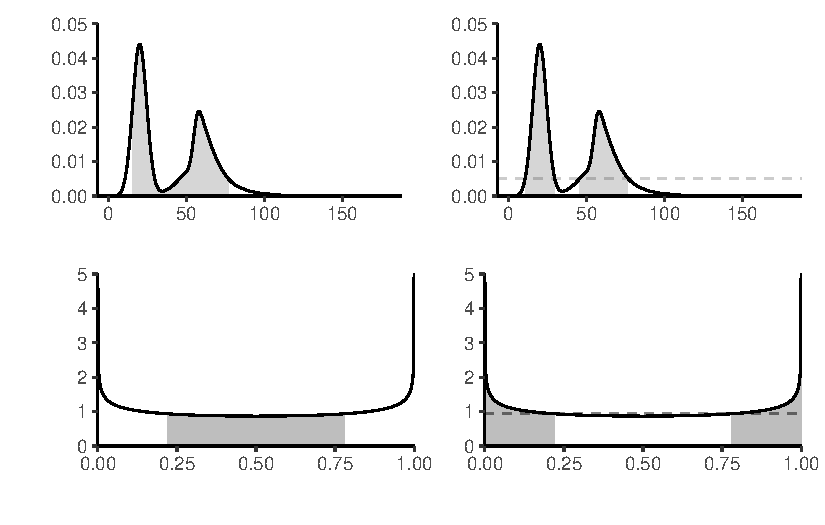
\includegraphics[keepaspectratio]{bayesics_files/figure-pdf/fig-credible-intervals-1.pdf}}

}

\caption{\label{fig-credible-intervals}Density plots with 89\% (top) and
50\% (bottom) equitailed or central credible (left) and highest
posterior density (right) regions for two data sets, highlighted in
grey. The horizontal lign gives the posterior density value determining
the cutoff for the HDP region.}

\end{figure}%

\begin{tcolorbox}[enhanced jigsaw, colframe=quarto-callout-important-color-frame, colback=white, leftrule=.75mm, opacitybacktitle=0.6, toprule=.15mm, colbacktitle=quarto-callout-important-color!10!white, title=\textcolor{quarto-callout-important-color}{\faExclamation}\hspace{0.5em}{\textbf{Summary}:}, left=2mm, breakable, titlerule=0mm, bottomrule=.15mm, opacityback=0, bottomtitle=1mm, rightrule=.15mm, arc=.35mm, toptitle=1mm, coltitle=black]

\begin{itemize}
\tightlist
\item
  Bayesians treat both parameter and observations as random, the former
  due to uncertainty about the true value. Inference is performed
  conditional on observed data, and summarized in the posterior.
\item
  Bayesians specify both a prior for the parameter, and a likelihood
  specifying the data generating mechanism. It is thus an extension of
  likelihood-based inference.
\item
  Information from the prior is updated in light of new data, which is
  encoded by the likelihood. Sequential updating leads.
\item
  Under weak conditions on the prior, large-sample behaviour of Bayesian
  and frequentist.
\item
  Bayesian inference is complicated by the fact that there is more often
  than not no closed-form expression for the posterior distribution.
  Evaluation of the normalizing constant, the so-called marginal
  likelihood, is challenging, especially in high dimensional settings.
\item
  Rather than hypothesis testing, Bayesian methods rely on the posterior
  distribution of parameters, or on Bayes factor for model comparisons.
\item
  The posterior predictive distribution, used for model assessment and
  prediction, and it has a higher variance than the data generating
  distribution from the likelihood, due to parameter uncertainty.
\item
  Bayesians typically will have approximations to the posterior
  distribution, or samples drawn from it.
\item
  Loss functions can be used to summarize a posterior distribution into
  a numerical summary of interest, which may vary depending on the
  objective.
\item
  Uncertainty is reflected by credible sets or credible intervals, which
  encode the posterior probability that the true value
  \(\boldsymbol{\theta}\) belongs to the set.
\end{itemize}

\end{tcolorbox}

\bookmarksetup{startatroot}

\chapter{Priors}\label{priors}

The posterior distribution combines two ingredients: the likelihood and
the prior. If the former is a standard ingredient of any
likelihood-based inference, prior specification requires some care. The
purpose of this chapter is to consider different standard way of
constructing prior functions, and to specify the parameters of the
latter: we term these hyperparameters.

The posterior is a compromise prior and likelihood: the more informative
the prior, the more the posterior resembles it, but in large samples,
the effect of the prior is often negligible if there is enough
information in the likelihood about all parameters. We can assess the
robustness of the prior specification through a sensitivity analysis by
comparing the outcomes of the posterior for different priors or
different values of the hyperparameters.

Oftentimes, we will specify independent priors in multiparameter models,
but the posterior of these will not be independent.

We can use moment matching to get sensible values, or tune via
trial-and-error using the prior predictive draws to assess the
implausibility of the prior outcomes. One challenge is that even if we
have some prior information (e.g., we can obtain sensible prior values
for the mean, quantiles or variance of the parameter of interest), these
summary statisticss will not typically be enough to fully characterize
the prior: many different functions or distributions could encode the
same information. This means that different analysts get different
inferences. Generally, we will choose the prior for convenience. Priors
are controversial because they could be tuned aposteriori to give any
answer an analyst might want.

\begin{tcolorbox}[enhanced jigsaw, colframe=quarto-callout-important-color-frame, colback=white, leftrule=.75mm, opacitybacktitle=0.6, toprule=.15mm, colbacktitle=quarto-callout-important-color!10!white, title=\textcolor{quarto-callout-important-color}{\faExclamation}\hspace{0.5em}{\textbf{Learning objectives}:}, left=2mm, breakable, titlerule=0mm, bottomrule=.15mm, opacityback=0, bottomtitle=1mm, rightrule=.15mm, arc=.35mm, toptitle=1mm, coltitle=black]

At the end of the chapter, students should be able to

\begin{itemize}
\tightlist
\item
  define and distinguish between improper, weak and informative priors.
\item
  propose conjugate priors for exponential families.
\item
  assess by using the prior predictive distribution the compatibility of
  the prior with the model.
\item
  use moment matching to specify the parameters of a prior distribution.
\item
  perform sensitivity analysis by running a model with different priors
  and assessing changes to the posterior distribution.
\end{itemize}

\end{tcolorbox}

\section{Prior simulation}\label{prior-simulation}

Expert elicitation is difficult and it is hard to grasp what the impacts
of the hyperparameters are. One way to see if the priors are reasonable
is to sample values from them and generate new observations, resulting
in prior predictive draws.

The prior predictive is
\(\int_{\boldsymbol{\Theta}} f(y_{\text{new}}; \boldsymbol{\theta}) p(\boldsymbol{\theta}) \mathrm{d} \boldsymbol{\theta}\):
we can simulate outcomes from it by first drawing parameter values
\(\boldsymbol{\theta}_0\) from the prior, then sampling new observations
from the distribution \(f(y_{\text{new}}; \boldsymbol{\theta}_0)\) with
those parameters values and keeping only \(y_{\text{new}}.\) If there
are sensible bounds for the range of the response, we could restrict the
prior range and shape until values abide to these.

Working with standardized inputs
\(x_i \mapsto (x_i - \overline{x})/\mathrm{sd}(\boldsymbol{x})\) is
useful. For example, in a simple linear regression (with a sole
numerical explanatory), the slope is the correlation between
standardized explanatory \(\mathrm{X}\) and standardized response \(Y\)
and the intercept should be mean zero.

\begin{example}[]\protect\hypertarget{exm-bixi-temp}{}\label{exm-bixi-temp}

Consider the daily number of Bixi bike sharing users for 2017--2019 at
the Edouard Montpetit station next to HEC: we can consider a simple
linear regression with log counts as a function of
temperature,\footnote{If counts are Poisson, then the log transform is
  variance stabilizing.}
\[\log (\texttt{nusers}) \sim \mathsf{Gauss}_{+}\{\beta_0 + \beta_1 (\texttt{temp}-20), \sigma^2\}.\]
The \(\beta_1\) slope measures units in degree Celsius per log number of
person.

The hyperparameters depend of course on the units of the analysis,
unless one standardizes response variable and explanatories: it is
easier to standardize the temperature so that we consider deviations
from, say 20\(^{\circ}\)C, which is not far from the observed mean in
the sample. After some tuning, the independent priors
\(\beta_0 \sim \mathsf{Gauss}(\overline{y}, 0.5^2),\)
\(\beta_1 \sim \mathsf{Gauss}(0, 0.05^2)\) and
\(\sigma \sim \mathsf{Exp}(3)\) seem to yield plausible outcomes and
relationships.\footnote{One can object to the prior parameters depending
  on the data, but an alternative would be to model centered data
  \(y-\overline{y},\) in which case the prior for the intercept
  parameter \(\beta_0\) would be zero.}

\begin{figure}[ht!]

\centering{

\pandocbounded{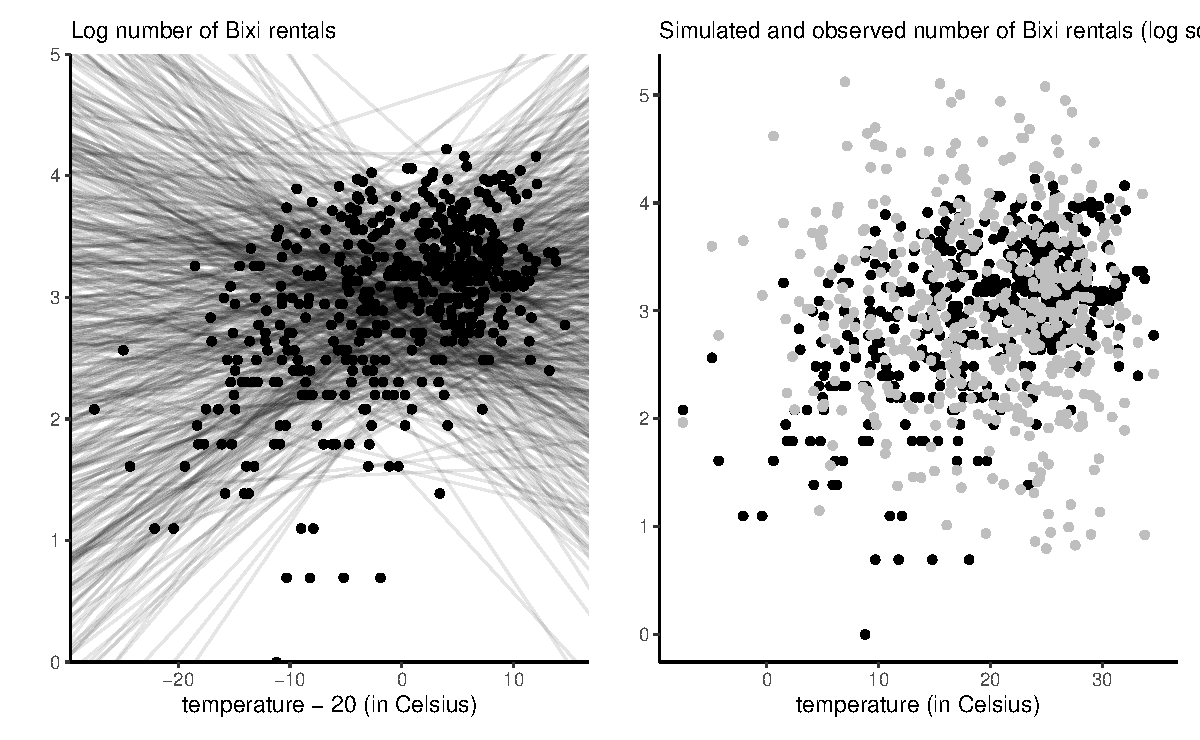
\includegraphics[keepaspectratio]{priors_files/figure-pdf/fig-bixi-1.pdf}}

}

\caption{\label{fig-bixi}Prior draws of the linear regressions with
observed data superimposed (left), and draws of observations from the
prior predictive distribution (in gray) against observed data (right).}

\end{figure}%

We can draw regression lines from the prior, as in the left panel of
Figure~\ref{fig-bixi}: while some of the negative relationships appear
unlikely after seeing the data, the curves all seem to pass somewhere in
the cloud of point. By contrast, a silly prior is one that would result
in all observations being above or below the regression line, or yield
values that are much too large near the endpoints of the explanatory
variable. Indeed, given the number of bikes for rental is limited (a
docking station has only 20 bikes), it is also sensible to ensure that
simulations do not return overly large numbers. The maximum number of
daily users in the sample is 68, so priors that return simulations with
more than 200 (rougly 5.3 on the log scale) are not that plausible. The
prior predictive draws can help establish this and the right panel of
Figure~\ref{fig-bixi} shows that, expect for the lack of correlation
between temperature and number of users, the simulated values from the
prior predictive are plausible even if overdispersed.

\end{example}

\section{Conjugate priors}\label{conjugate-priors}

In very simple models, there may exists prior densities that result in a
posterior distribution of the same family. We can thus directly extract
characteristics of the posterior. Conjugate priors are chosen for
computational convenience and because interpretation is convenient, as
the parameters of the posterior will often be some weighted average of
prior and likelihood component.

\begin{definition}[Conjugate
priors]\protect\hypertarget{def-conjugate-prior}{}\label{def-conjugate-prior}

A prior density \(p(\boldsymbol{\theta})\) is conjugate for likelihood
\(L(\boldsymbol{\theta}; \boldsymbol{y})\) if the product
\(L(\boldsymbol{\theta}; \boldsymbol{y})p(\boldsymbol{\theta}),\) after
renormalization, is of the same parametric family as the prior.

Exponential families (see Definition~\ref{def-exponential-family},
including the binomial, Poisson, exponential, Gaussian distributions)
admit conjugate priors.

\begin{longtable}[]{@{}
  >{\raggedright\arraybackslash}p{(\linewidth - 4\tabcolsep) * \real{0.3455}}
  >{\raggedright\arraybackslash}p{(\linewidth - 4\tabcolsep) * \real{0.3273}}
  >{\raggedright\arraybackslash}p{(\linewidth - 4\tabcolsep) * \real{0.3273}}@{}}
\toprule\noalign{}
\begin{minipage}[b]{\linewidth}\raggedright
distribution
\end{minipage} & \begin{minipage}[b]{\linewidth}\raggedright
unknown parameter
\end{minipage} & \begin{minipage}[b]{\linewidth}\raggedright
conjugate prior
\end{minipage} \\
\midrule\noalign{}
\endhead
\bottomrule\noalign{}
\endlastfoot
\(Y \sim \mathsf{expo}(\lambda)\) & \(\lambda\) &
\(\lambda \sim \mathsf{gamma}(\alpha, \beta)\) \\
\(Y \sim \mathsf{Poisson}(\mu)\) & \(\mu\) &
\(\mu \sim \mathsf{gamma}(\alpha, \beta)\) \\
\(Y \sim \mathsf{binom}(n, \theta)\) & \(\theta\) &
\(\theta \sim \mathsf{Be}(\alpha, \beta)\) \\
\(Y \sim \mathsf{Gauss}(\mu, \sigma^2)\) & \(\mu\) &
\(\mu \sim \mathsf{Gauss}(\nu, \omega^2)\) \\
\(Y \sim \mathsf{Gauss}(\mu, \sigma^2)\) & \(\sigma\) &
\(\sigma^{2} \sim \mathsf{inv. gamma}(\alpha, \beta)\) \\
\(Y \sim \mathsf{Gauss}(\mu, \sigma^2)\) & \(\mu, \sigma\) &
\(\mu \mid \sigma^2 \sim \mathsf{Gauss}(\nu, \omega \sigma^2),\)
\(\sigma^{2} \sim \mathsf{inv. gamma}(\alpha, \beta)\) \\
\end{longtable}

\end{definition}

\begin{example}[Conjugate prior for the binomial
model]\protect\hypertarget{exm-conjugatepriors-binom}{}\label{exm-conjugatepriors-binom}

Since the density of the binomial is of the form \(p^y(1-p)^{n-y}\) and
it belongs to an exponential family
(Example~\ref{exm-exponential-family-binom}), the beta distribution
\(\mathsf{beta}(\alpha, \beta)\) with density
\[f(x) \propto x^{\alpha-1} (1-x)^{\beta-1}\] is the conjugate prior.

The beta distribution is also the conjugate prior for the negative
binomial, geometric and Bernoulli distributions, since their likelihoods
are all proportional to that of the beta. The fact that different
sampling schemes that result in proportional likelihood functions give
the same inference is called likelihood principle.

\end{example}

\begin{example}[Conjugate prior for the Poisson
model]\protect\hypertarget{exm-conjugatepriors-poisson}{}\label{exm-conjugatepriors-poisson}

We saw in Example~\ref{exm-exponential-family-poisson} that the Poisson
distribution is an exponential family. The gamma density,
\[ f(x) \propto \beta^{\alpha}/\Gamma(\alpha)x^{\alpha-1} \exp(-\beta x)\]
with shape \(\alpha\) and rate \(\beta\) is the conjugate prior for the
Poisson. For an \(n\)-sample of independent observations
\(\mathsf{Poisson}(\mu)\) observations with
\(\mu \sim \mathsf{gamma}(\alpha, \beta),\) the posterior is
\(\mathsf{gamma}(\sum_{i=1}^n y_i + \alpha, \beta + n).\)

\end{example}

Knowing the analytic expression for the posterior can be useful for
calculations of the marginal likelihood, as
Example~\ref{exm-poisson-negbin} demonstrated.

\begin{example}[Posterior rates for A/B tests using conjugate Poisson
model]\protect\hypertarget{exm-abtest}{}\label{exm-abtest}

Upworthy.com, a US media publisher, revolutionized headlines online
advertisement by running systematic A/B tests to compare the different
wording of headlines, placement and image and what catches attention the
most. The Upworthy Research Archive (\citeproc{ref-Matias:2021}{Matias
et al. 2021}) contains results for 22743 experiments, with a click
through rate of 1.58\% on average and a standard deviation of 1.23\%.
The \texttt{clickability\_test\_id} gives the unique identifier of the
experiment, \texttt{clicks} the number of conversion out of
\texttt{impressions}. See
\href{https://tellingstorieswithdata.com/08-hunt.html\#ab-testing}{Section
8.5} of Alexander (\citeproc{ref-Alexander:2023}{2023}) for more details
about A/B testing and background information.

Consider an A/B test from November 23st, 2014, that compared four
different headlines for a story on Sesame Street workshop with
interviews of children whose parents were in jail and visiting them in
prisons. The headlines tested were:

\begin{quote}
\begin{enumerate}
\def\labelenumi{\arabic{enumi}.}
\tightlist
\item
  Some Don't Like It When He Sees His Mom. But To Him? Pure Joy. Why
  Keep Her From Him?
\item
  They're Not In Danger. They're Right. See True Compassion From The
  Children Of The Incarcerated.
\item
  Kids Have No Place In Jail \ldots{} But In This Case, They
  \emph{Totally} Deserve It.
\item
  Going To Jail \emph{Should} Be The Worst Part Of Their Life. It's So
  Not. Not At All.
\end{enumerate}
\end{quote}

At first glance, the first and third headlines seem likely to lead to a
curiosity gap. The wording of the second is more explicit (and
searchable), whereas the first is worded as a question.

We model the conversion rate \(\lambda_i\) for each headline separately
using a Poisson distribution and compare the posterior distributions for
all four choices. Using a conjugate prior and selecting the parameters
by moment matching yields approximately \(\alpha = 1.65\) and
\(\beta = 104.44\) for the hyperparameters, setting
\(\alpha/\beta = 0.0158\) and \(\alpha/\beta^2=0.0123^2\) and solving
for the two unknown parameters.

\begin{longtable}[]{@{}lrr@{}}

\caption{\label{tbl-upworthy}Number of views, clicks for different
headlines for the Upworthy data.}

\tabularnewline

\toprule\noalign{}
headline & impressions & clicks \\
\midrule\noalign{}
\endhead
\bottomrule\noalign{}
\endlastfoot
H1 & 3060 & 49 \\
H2 & 2982 & 20 \\
H3 & 3112 & 31 \\
H4 & 3083 & 9 \\

\end{longtable}

\begin{figure}[ht!]

\centering{

\pandocbounded{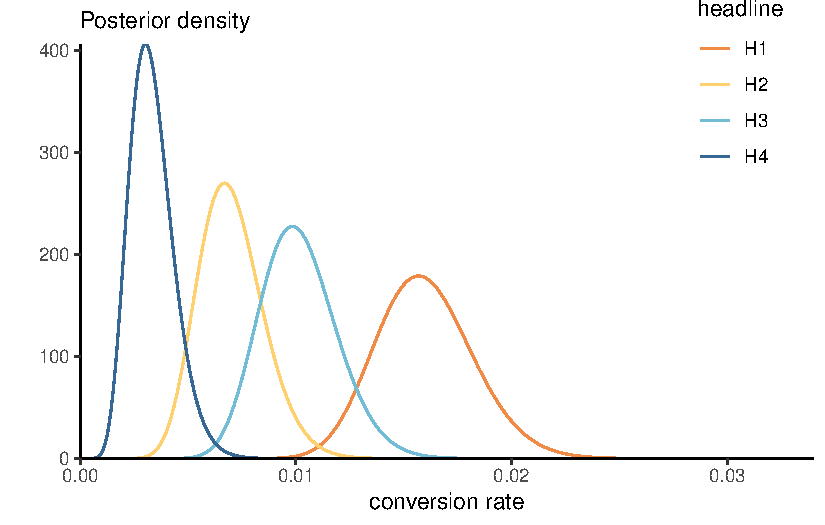
\includegraphics[keepaspectratio]{priors_files/figure-pdf/fig-upworthy-1.pdf}}

}

\caption{\label{fig-upworthy}Gamma posterior for conversion rate of the
different Upworthy Sesame Street headline.}

\end{figure}%

We can visualize the posterior distributions. In this context, the large
sample size lead to the dominance of the likelihood contribution
\(p(Y_i \mid \lambda_i) \sim \mathsf{Poisson}(n_i\lambda_i)\) relative
to the prior. We can see there is virtually no overlap between different
rates for headers H1 (preferred) relative to H4 (least favorable). The
probability that the conversion rate for Headline 3 is higher than
Headline 1 can be approximated by simulating samples from both
posteriors and computing the proportion of times one is larger: we get
2\% for \texttt{H3} relative to \texttt{H1}, indicating a clear
preference for the first headline \texttt{H1}.

\end{example}

\begin{example}[Should you phrase your headline as a
question?]\protect\hypertarget{exm-poisson-upworthy-question}{}\label{exm-poisson-upworthy-question}

We can also consider aggregate records for Upworthy, as Alexander
(\citeproc{ref-Alexander:2023}{2023}) did. The
\texttt{upworthy\_question} database contains a balanced sample of all
headlines where at least one of the choices featured a question, with at
least one alternative statement. Whether a headline contains a question
or not is determined by querying for the question mark. We consider
aggregated counts for all such headlines, with the \texttt{question}
factor encoding whether there was a question, \texttt{yes} or
\texttt{no}. For simplicity, we treat the number of views as fixed, but
keep in mind that A/B tests are often sequential experiments with a
stopping rule.\footnote{The stopping rule means that data stops being
  collected once there is enough evidence to determine if an option is
  more suitable, or if a predetermined number of views has been reached.}

We model first the rates using a Poisson regression; the corresponding
frequentist analysis would include an offset to account for differences
in views. If \(\lambda_{j}\) \((j=1, 2)\) are the average rate for each
factor level (yes and no), then
\(\mathsf{E}(Y_{ij}/n_{ij}) = \lambda_j.\) In the frequentist setting,
we can fit a simple Poisson generalized linear regression model with an
offset term and a binary variable.

\begin{Shaded}
\begin{Highlighting}[]
\FunctionTok{data}\NormalTok{(upworthy\_question, }\AttributeTok{package =} \StringTok{"hecbayes"}\NormalTok{)}
\NormalTok{poismod }\OtherTok{\textless{}{-}} \FunctionTok{glm}\NormalTok{(}
\NormalTok{  clicks }\SpecialCharTok{\textasciitilde{}} \FunctionTok{offset}\NormalTok{(}\FunctionTok{log}\NormalTok{(impressions)) }\SpecialCharTok{+}\NormalTok{ question, }
  \AttributeTok{family =} \FunctionTok{poisson}\NormalTok{(}\AttributeTok{link =} \StringTok{"log"}\NormalTok{),}
  \AttributeTok{data =}\NormalTok{ upworthy\_question)}
\FunctionTok{coef}\NormalTok{(poismod)}
\end{Highlighting}
\end{Shaded}

\begin{verbatim}
(Intercept)  questionno 
-4.51264669  0.07069677 
\end{verbatim}

The coefficients represent the difference in log rate (multiplicative
effect) relative to the baseline rate, with an increase of 6.3 percent
when the headline does not contain a question. A likelihood ratio test
can be performed by comparing the deviance of the null model
(intercept-only), indicating strong evidence that including question
leads to significatively different rates. This is rather unsurprising
given the enormous sample sizes.

Consider instead a Bayesian analysis with conjugate prior: we model
separately the rates of each group (question or not). Suppose we think
apriori that the click-rate is on average 1\%, with a standard deviation
of 2\%, with no difference between questions or not. For a
\(\mathsf{Gamma}(\alpha, \beta)\) prior, this would translate, using
moment matching, into a rate of
\(\beta = 25 = \mathsf{E}_0(\lambda_j)/ \mathsf{Var}_0(\lambda_j)\) and
a shape of \(\alpha = 0.25\) (\(j=1, 2\)). If \(\lambda_{j}\) is the
average rate for each factor level (yes and no), then
\(\mathsf{E}(Y_{ij}/n_{ij}) = \lambda_j\) so the log likelihood is
proportional, as a function of \(\lambda_1\) and \(\lambda_2,\) to
\begin{align*}
\ell(\boldsymbol{\lambda}; \boldsymbol{y}, \boldsymbol{n}) \stackrel{\boldsymbol{\lambda}}{\propto} \sum_{i=1}^n \sum_{j=1}^2 y_{ij}\log \lambda_j - \lambda_jn_{ij}
\end{align*} and we can recognize that the posterior for \(\lambda_i\)
is gamma with shape \(\alpha + \sum_{i=1}^n y_{ij}\) and rate
\(\beta + \sum_{i=1}^n n_{ij}.\) For inference, we thus only need to
select hyperparameters and calculate the total number of clicks and
impressions per group. We can then consider the posterior difference
\(\lambda_1 - \lambda_2\) or, to mimic the Poisson multiplicative model,
of the ratio \(\lambda_1/\lambda_2.\) The former suggests very small
differences, but one must keep in mind that rates are also small. The
ratio, shown in the right-hand panel of
Figure~\ref{fig-hist-difference_rates}, gives a more easily
interpretable portrait that is in line with the frequentist analysis.

\begin{figure}[ht!]

\centering{

\pandocbounded{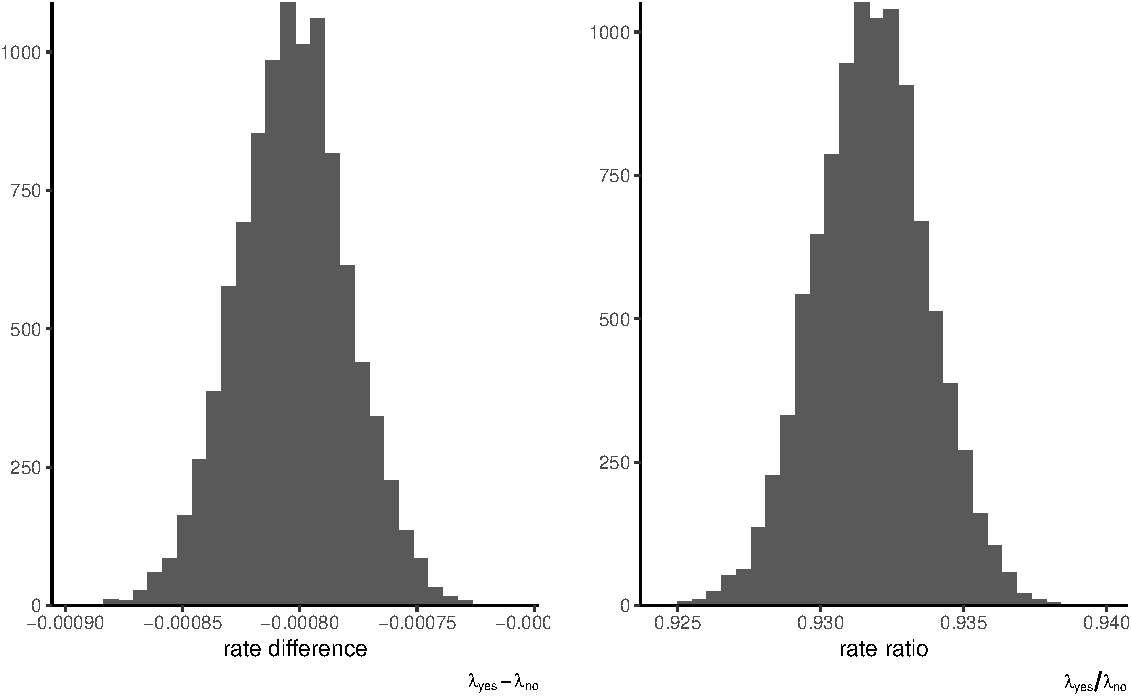
\includegraphics[keepaspectratio]{priors_files/figure-pdf/fig-hist-difference_rates-1.pdf}}

}

\caption{\label{fig-hist-difference_rates}Histograms of posterior
summaries for differences (left) and rates (right) based on 1000
simulations from the independent gamma posteriors.}

\end{figure}%

To get an approximation to the posterior mean of the ratio
\(\lambda_1/\lambda_2,\) it suffices to draw independent observations
from their respective posterior, compute the ratio and take the sample
mean of those draws. We can see that the sampling distribution of the
ratio is nearly symmetrical, so we can expect Wald intervals to perform
well should one be interested in building confidence intervals. This is
however hardly surprising given the sample size at play.

\end{example}

\begin{example}[Conjugate prior for Gaussian mean with known
variance]\protect\hypertarget{exm-conjugatepriors-normal}{}\label{exm-conjugatepriors-normal}

Consider an \(n\) simple random sample of independent and identically
distributed Gaussian variables with mean \(\mu\) and standard deviation
\(\sigma,\) denoted \(Y_i \sim \mathsf{Gauss}(\mu, \sigma^2).\) We pick
a Gaussian prior for the location parameter,
\(\mu \sim \mathsf{Gauss}(\nu, \tau^2)\) where we assume \(\nu, \tau\)
are fixed hyperparameter values. For now, we consider only inference for
the conditional marginal posterior
\(p(\mu \mid \boldsymbol{y}, \sigma)\): discarding any term that is not
a function of \(\mu,\) the conditional posterior is \begin{align*}
p(\mu \mid \sigma, \boldsymbol{y}) &\propto \exp\left\{ -\frac{1}{2\sigma^2}\sum_{i=1}^n (y_{i}-\mu)^2\right\} \exp\left\{-\frac{1}{2\tau^2}(\mu - \nu)^2\right\}
\\&\propto \exp\left\{\left(\frac{\sum_{i=1}^n y_{i}}{\sigma^2} + \frac{\nu}{\tau^2}\right)\mu - \left( \frac{n}{2\sigma^2} +\frac{1}{2\tau^2}\right)\mu^2\right\}.
\end{align*} The log of the posterior density conditional on \(\sigma\)
is quadratic in \(\mu,\) it must be a Gaussian distribution truncated
over the positive half line. This can be seen by completing the square
in \(\mu,\) or by comparing this expression to the density of
\(\mathsf{Gauss}(\mu, \sigma^2),\) \begin{align*}
f(x; \mu, \sigma) \stackrel{\mu}{\propto} \exp\left(-\frac{1}{2 \sigma^2}\mu^2 + \frac{x}{\sigma^2}\mu\right)
\end{align*} we can deduce by matching mean and variance that the
conditional posterior \(p(\mu \mid \sigma)\) is Gaussian with reciprocal
variance (precision) \(n/\sigma^2 + 1/\tau^2\) and mean
\((n\overline{y}\tau^2 + \nu \sigma^2)/(n\tau^2 + \sigma^2).\) The
precision is an average of that of the prior and data, but assigns more
weight to the latter, which increases linearly with the sample size
\(n.\) Likewise, the posterior mean is a weighted average of prior and
sample mean, with weights proportional to the relative precision.

\end{example}

The exponential family is quite large;
\href{https://www.johndcook.com/CompendiumOfConjugatePriors.pdf}{Fink
(1997) \emph{A Compendium of Conjugate Priors}} gives multiple examples
of conjugate priors and work out parameter values.

In general, unless the sample size is small and we want to add expert
opinion, we may wish to pick an \emph{uninformative prior}, i.e., one
that does not impact much the outcome. For conjugate models, one can
often show that the relative weight of prior parameters (relative to the
random sample likelihood contribution) becomes negligible by
\href{https://en.wikipedia.org/wiki/Conjugate_prior}{investigating their
relative weights}.

\section{Uninformative priors}\label{uninformative-priors}

\begin{definition}[Proper
prior]\protect\hypertarget{def-properprior}{}\label{def-properprior}

We call a prior function \emph{proper} if it's integral is finite over
the parameter space; such prior function automatically leads to a valid
posterior. A prior over \(\boldsymbol{\Theta}\) is \textbf{improper} if
\(\int_{\boldsymbol{\Theta}} p(\boldsymbol{\theta}) \mathrm{d} \boldsymbol{\theta} = \infty.\)

\end{definition}

The best example of proper priors arise from probability density
function. We can still employ this rule for improper priors: for
example, taking \(\alpha, \beta \to 0\) in the beta prior leads to a
prior proportional to \(x^{-1}(1-x)^{-1},\) the integral of which
diverges on the unit interval \([0,1].\) However, as long as the number
of success and the number of failures is larger than 1, meaning
\(k \geq 1, n-k \geq 1,\) the posterior distribution would be proper,
i.e., integrable. To find the posterior, normalizing constants are also
superfluous.

Many uninformative priors are flat, or proportional to a uniform on some
subset of the real line and therefore improper. It may be superficially
tempting to set a uniform prior on a large range to ensure posterior
property, but the major problem is that a flat prior may be informative
in a different parametrization, as the following example suggests.

Gelman et al. (\citeproc{ref-Gelman:2013}{2013}) uses the following
taxonomy for various levels of prior information:

\begin{itemize}
\tightlist
\item
  uninformative priors are generally flat or uniform priors with
  \(p(\beta) \propto 1.\)
\item
  vague priors are typically nearly flat even if proper, e.g.,
  \(\beta \sim \mathsf{Gauss}(0, 100),\)
\item
  weakly informative priors provide little constraints
  \(\beta \sim \mathsf{Gauss}(0, 10),\) and
\item
  informative prior are typically application-specific, but constrain
  the ranges.
\end{itemize}

Uninformative and vague priors are generally not recommended unless they
are known to give valid posterior inference and the amount of
information from the likelihood is high.

\begin{example}[Transformation of flat prior for
scales]\protect\hypertarget{exm-scaleflatprior}{}\label{exm-scaleflatprior}

Consider the parameter \(\log(\tau) \in \mathbb{R}\) and the prior
\(p( \log \tau) \propto 1.\) If we reparametrize the model in terms of
\(\tau,\) the new prior (including the Jacobian of the transformation)
is \(\tau^{-1}\)

\end{example}

Some priors are standard and widely used. In location scale families
with location \(\nu\) and scale \(\tau,\) the density is such that
\begin{align*}
f(x; \nu, \tau) =  \frac{1}{\tau} f\left(\frac{x - \nu}{\tau}\right), \qquad \nu \in \mathbb{R}, \tau >0.
\end{align*} We thus wish to have a prior so that
\(p(\tau) = c^{-1}p(\tau/c)\) for any scaling \(c>0,\) whence it follows
that \(p(\tau) \propto \tau^{-1},\) which is uniform on the log scale.

The priors \(p(\nu) \propto 1\) and \(p(\tau) \propto \tau^{-1}\) are
both improper but lead to location and scale invariance, hence that the
result is the same regardless of the units of measurement.

One criticism of the Bayesian approach is the arbitrariness of prior
functions. However, the role of the prior is often negligible in large
samples (consider for example the posterior of exponential families with
conjugate priors). Moreover, the likelihood is also chosen for
convenience, and arguably has a bigger influence on the conclusion. Data
fitted using a linear regression model seldom follow Gaussian
distributions conditionally, in the same way that the linearity is a
convenience (and first order approximation).

\begin{definition}[Jeffrey's
prior]\protect\hypertarget{def-jeffreys}{}\label{def-jeffreys}

In single parameter models, taking a prior function for \(\theta\)
proportional to the square root of the determinant of the information
matrix, \(p(\theta) \propto |\imath(\theta)|^{1/2}\) yields a prior that
is invariant to reparametrization, so that inferences conducted in
different parametrizations are equivalent.\footnote{The Fisher
  information is linear in the sample size for independent and
  identically distributed data so we can derive the result for \(n=1\)
  without loss of generality.}

To see this, consider a bijective transformation
\(\theta \mapsto \vartheta.\) Under the reparametrized model and
suitable regularity conditions\footnote{Using Bartlett's identity;
  Fisher consistency can be established using the dominated convergence
  theorem.}, the chain rule implies that \begin{align*}
i(\vartheta) &= - \mathsf{E} \left(\frac{\partial^2 \ell(\vartheta)}{\partial^2 \vartheta}\right)
\\&= - \mathsf{E}\left(\frac{\partial^2 \ell(\theta)}{\partial \theta^2}\right) \left( \frac{\mathrm{d} \theta}{\mathrm{d} \vartheta} \right)^2 + \mathsf{E}\left(\frac{\partial \ell(\theta)}{\partial \theta}\right) \frac{\mathrm{d}^2 \theta}{\mathrm{d} \vartheta^2}
\end{align*} Since the score has mean zero,
\(\mathsf{E}\left\{\partial \ell(\theta)/\partial \theta\right\}=0\) and
the rightmost term vanishes. We can thus relate the Fisher information
in both parametrizations, with \begin{align*}
\imath^{1/2}(\vartheta) = \imath^{1/2}(\theta) \left| \frac{\mathrm{d} \theta}{\mathrm{d} \vartheta} \right|,
\end{align*} implying invariance.

In multiparameter models, the system isn't invariant to
reparametrization if we consider the determinant of the Fisher
information.

\end{definition}

\begin{example}[Jeffrey's prior for the binomial
distribution]\protect\hypertarget{exm-jeffreysbinom}{}\label{exm-jeffreysbinom}

Consider the binomial distribution \(\mathsf{Bin}(1, \theta)\) with
density
\(f(y; \theta) \propto  \theta^y(1-\theta)^{1-y}\mathbf{1}_{\theta \in [0,1]}.\)
The negative of the second derivative of the log likelihood with respect
to \(p\) is
\[\jmath(\theta) = - \partial^2 \ell(\theta; y) / \partial \theta^2 = y/\theta^2 + (1-y)/(1-\theta)^2\]
and since \(\mathsf{E}(Y)=\theta,\) the Fisher information is
\[\imath(\vartheta) = \mathsf{E}\{\jmath(\theta)\}=1/\theta + 1/(1-\theta) = 1/\{\theta(1-\theta)\}\]
Jeffrey's prior is thus
\(p(\theta) \propto \theta^{-1/2}(1-\theta)^{-1/2},\) a conjugate Beta
prior \(\mathsf{beta}(0.5,0.5).\)

\end{example}

\begin{exercise}[Jeffrey's prior for the normal
distribution]\protect\hypertarget{exr-jeffreysnormal}{}\label{exr-jeffreysnormal}

Check that for the Gaussian distribution
\(\mathsf{Gauss}(\mu, \sigma^2),\) the Jeffrey's prior obtained by
treating each parameter as fixed in turn, are \(p(\mu) \propto 1\) and
\(p(\sigma) \propto 1/\sigma,\) which also correspond to the default
uninformative priors for location-scale families.

\end{exercise}

\begin{example}[Jeffrey's prior for the Poisson
distribution]\protect\hypertarget{exm-jeffreyspoisson}{}\label{exm-jeffreyspoisson}

The Poisson distribution with
\(\ell(\lambda) \propto -\lambda + y\log \lambda,\) with second
derivative
\(-\partial^2 \ell(\lambda)/\partial \lambda^2 = y/\lambda^2.\) Since
the mean of the Poisson distribution is \(\lambda,\) the Fisher
information is \(\imath(\lambda) = \lambda^{-1}\) and Jeffrey's prior is
\(\lambda^{-1/2}.\)

\end{example}

\section{Priors for regression
models}\label{priors-for-regression-models}

Regression models often feature Gaussian priors on the mean coefficients
\(\boldsymbol{\beta},\) typically chosen to be vague with large
variance. Below are some alternatives, many of which aim to enforce
shrinkage towards zero, or sparsity.

\begin{proposition}[Zellner's \(g\)
prior]\protect\hypertarget{prp-Zellner-g-prior}{}\label{prp-Zellner-g-prior}

Consider an ordinary linear regression model for
\(\boldsymbol{Y} \sim \mathsf{Gauss}_n(\beta_0\mathbf{1}_n + \mathbf{X}\boldsymbol{\beta}, \sigma^2 \mathbf{I}_n),\)
with intercept \(\beta_0\) and mean coefficient vector
\(\boldsymbol{\beta} = (\beta_1, \ldots, \beta_p)^\top\) associated to
the model matrix \(\mathbf{X}.\) Zellner
(\citeproc{ref-Zellner:1986}{1986})'s \(g\) prior consists in letting
\(\boldsymbol{\beta} \sim \mathsf{Gauss}_p\{\boldsymbol{0}_p, g \sigma^2(\mathbf{X}^\top\mathbf{X})^{-1}\},\)
where \(g>0\) is a constant.

The ordinary least square estimator of the mean coefficients satisfies
under regularity conditions on the model matrix
\(\widehat{\boldsymbol{\beta}} \sim \mathsf{Gauss}_p\{\boldsymbol{\beta}, \sigma^2(\mathbf{X}^\top\mathbf{X})^{-1}\}\)
for Gaussian data, whence we get the closed-form conditional
distributions \begin{align*}
\beta_0 \mid \sigma^2, \boldsymbol{Y} &\sim \mathsf{Gauss}(\overline{y}, \sigma^2/n)\\
\boldsymbol{\beta} \mid \beta_0, \sigma^2, \boldsymbol{Y} & \sim \mathsf{Gauss}_p\left\{\frac{g}{g+1} \widehat{\boldsymbol{\beta}}, \frac{g}{g+1}\sigma^2 (\mathbf{X}^\top\mathbf{X})^{-1}\right\} 
\end{align*} where \(\overline{y} = \boldsymbol{y}^\top\mathbf{1}_n/n\)
is the sample mean of the observed response vector. We can interpret
\(g>0\) as a prior weight, with the posterior conditional mean giving
weight of \(n/g\) to ``phantom (prior) observations'' with mean zero,
relative to the \(n\) observations in the observed sample: the ratio
\(g/(g+1)\) is called \textbf{shrinkage factor}.

By virtue of Proposition~\ref{prp-conditional-gaussian}, the prior is
also closed under conditioning, which is useful for model comparison
using Bayes factors. Consider a partition
\(\boldsymbol{\beta} = (\boldsymbol{\beta}_1^\top, \boldsymbol{\beta}_2^\top)^\top\)
of the mean coefficients and similarly the block of columns from the
model matrix, say \(\mathbf{X} = [\mathbf{X}_1\; \mathbf{X}_2]\) for
blocks of size \(k\) and \(p-k.\) If we remove \(p-k\) regressors from
the model setting \(\boldsymbol{\beta}_2=0,\) then the conditional is
\[\boldsymbol{\beta}_{1} \mid \boldsymbol{\beta}_2=\boldsymbol{0}_{p-k} \sim \mathsf{Gauss}_k\{\boldsymbol{0}_k, g\sigma^2 (\mathbf{X}_1^\top\mathbf{X}_1)^{-1}\},\]
which is the \(g\) prior for the submodel in which we omit the columns
corresponding to \(\mathbf{X}_2.\)

\end{proposition}

\section{Informative priors}\label{informative-priors}

One strength of the Bayesian approach is the capability of incorporating
expert and domain-based knowledge through priors. Often, these will take
the form of moment constraints, so one common way to derive a prior is
to perform moment matching to related elicited quantities with moments
of the prior distribution. It may be easier to set priors on a different
scale than those of the observations, as Example~\ref{exm-colestawn}
demonstrates.

\begin{example}[Gamma quantile difference priors for extreme value
distributions]\protect\hypertarget{exm-colestawn}{}\label{exm-colestawn}

The generalized extreme value distribution arises as the limiting
distribution for the maximum of \(m\) independent observations from some
common distribution \(F.\) The \(\mathsf{GEV}(\mu, \sigma, \xi)\)
distribution is a location-scale with distribution function
\begin{align*}
F(x) = \exp\left[ - \left\{1+\xi(x-\mu)/\sigma\right\}^{-1/\xi}_{+}\right]
\end{align*} where \(x_{+} = \max\{0, x\}.\)

Inverting the distribution function yields the quantile function
\begin{align*}
Q(p) \mu + \sigma \frac{(-\log p)^{-\xi}-1}{\xi}
\end{align*}

In environmental data, we often model annual maximum. Engineering
designs are often specified in terms of the \(k\)-year return levels,
defined as the quantile of the annual maximum exceeded with probability
\(1/k\) in any given year. Using a \(\mathsf{GEV}\) for annual maximum,
Coles and Tawn (\citeproc{ref-Coles.Tawn:1996}{1996}) proposed modelling
annual daily rainfall and specifying a prior on the quantile scale
\(q_1 < q_2 < q_3\) for tail probabilities \(p_1> p_2 > p_3.\) To deal
with the ordering constraints, gamma priors are imposed on the
differences

\begin{itemize}
\tightlist
\item
  \(q_1 - o \sim \mathsf{gamma}(\alpha_1, \beta_1),\)
\item
  \(q_2 - q_1 \sim \mathsf{gamma}(\alpha_2, \beta_2)\) and
\item
  \(q_3-q_2 \sim \mathsf{gamma}(\alpha_3, \beta_3),\)
\end{itemize}

where \(o\) is the lower bound of the support. The prior is thus of the
form \begin{align*}
p(\boldsymbol{q}) \propto q_1^{\alpha_1-1}\exp(-\beta_1 q_1) \prod_{i=2}^3 (q_i-q_{i-1})^{\alpha_i-1} \exp\{\beta_i(q_i-q_{i-1})\}.
\end{align*} where \(0 \leq q_1 \leq q_2 \leq q_3.\) The fact that these
quantities refer to moments or risk estimates which practitioners often
must compute as part of regulatory requirements makes it easier to
specify sensible values for hyperparameters.

\end{example}

\begin{example}[Priors in extreme value
theory]\protect\hypertarget{exm-martins}{}\label{exm-martins}

The generalized extreme value distribution obtained as the limit of
maximum of blocks of size \(m\) when suitably normalizes is a
location-scale family with a shape parameter \(\xi \in \mathbb{R}\). The
latter describes the heavyness of the tail, with negative values
corresponding to approximation by bounded upper tail distributions (such
as the beta), \(\xi=0\) to exponential tail decay and \(\xi>0\) to
polynomial tails, with finite moments of order \(1/\xi\). For example,
the Cauchy or Student-\(t\) distribution with one degree of freedom has
infinite first moment and \(\xi=1\).

In practice, the maximum likelihood estimators do not exist if
\(\xi < -1\) as the model is nonregular (\citeproc{ref-Smith:1985}{Smith
1985}), and the cumulant of order \(k\) exists only if \(\xi > -1/k\);
the Fisher information matrix exists only when \(\xi > -1/2\). Thus,
informative priors that restrict the range of the shape, may be useful
as in environmental applications the shapes would be in the vicinity of
zero. Martins and Stedinger
(\citeproc{ref-Martins.Stedinger:2000}{2000}) proposed a prior of the
form \begin{align*}
p(\xi) =\frac{(0.5+\xi)^{p-1}(0.5-\xi)^{q-1}}{\mathrm{beta}(p,q)}, \qquad \xi \in [-0.5, 0.5]
\end{align*} a shifted \(\mathsf{beta}(p,q)\) prior.

On the contrary, the \textbf{maximal data information} (MDI) prior
(\citeproc{ref-Zellner:1971}{Zellner 1971}) is defined in terms of
entropy,
\[p(\boldsymbol{\theta}) = \exp \mathsf{E}\{\log f(Y \mid \boldsymbol{\theta})\}.\]
It is an objective prior that reflects little about the parameter and
leads to inferences that have good frequentist property.

For the generalized Pareto distribution, \(p(\xi) \propto \exp(-\xi)\).
In this particular case, however, it is improper without modification
since \(\lim_{\xi \to -\infty} \exp(-\xi) = \infty\), and the prior
density increases without bound as \(\xi\) becomes smaller.

\begin{figure}[ht!]

\centering{

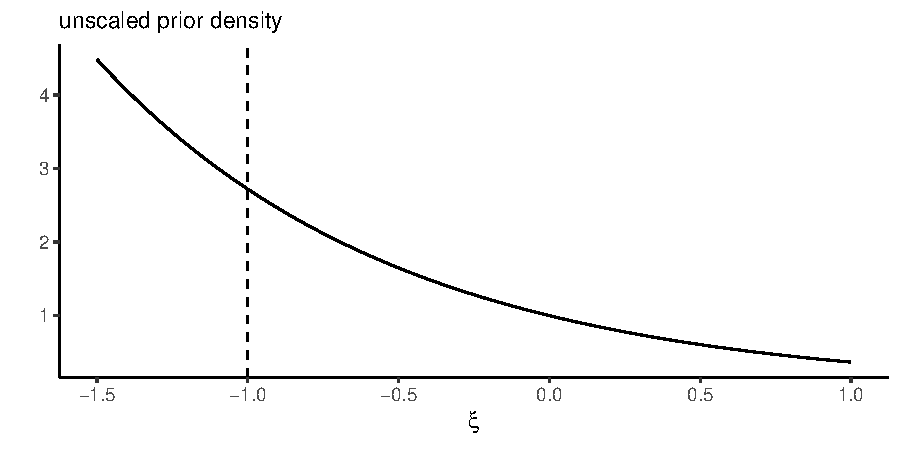
\includegraphics[width=1\linewidth,height=\textheight,keepaspectratio]{priors_files/figure-pdf/fig-mdiprior-1.pdf}

}

\caption{\label{fig-mdiprior}Unscaled maximum data information (MDI)
prior density.}

\end{figure}%

If we restrict the range of the MDI prior \(p(\xi)\) to \(\xi \geq -1\),
then \(p(\xi + 1) \sim \mathsf{expo}(1)\) and the resulting posterior is
proper (\citeproc{ref-Northrop.Attalides:2016}{Northrop and Attalides
2016, Zhang.Shaby:2023}). While being ``objective'', it is perhaps not
much suitable as it puts mass towards lower values of the shape, an
undesirable feature.

\end{example}

What would you do if we you had prior information from different
sources? One way to combine these is through a mixture: given \(M\)
different prior distributions \(p_m(\boldsymbol{\theta}),\) we can
assign each a positive weight \(w_m\) to form a mixture of experts prior
through the linear combination
\[ p(\boldsymbol{\theta}) \propto \sum_{m=1}^M w_m p_m(\boldsymbol{\theta})\]

\begin{proposition}[Penalized complexity
priors]\protect\hypertarget{prp-penalized-complexity}{}\label{prp-penalized-complexity}

Oftentimes, there will be a natural family of prior density to impose on
some model component, \(p(\boldsymbol{\theta} \mid \zeta),\) with
hyperparameter \(\zeta.\) The flexibility of the underlying construction
leads itself to overfitting. Penalized complexity priors
(\citeproc{ref-Simpson:2017}{Simpson et al. 2017}) aim to palliate this
by penalizing models far away from a simple baseline model, which
correspond to a fixed value \(\zeta_0.\) The prior will favour the
simpler parsimonious model the more prior mass one places on
\(\zeta_0,\) which is in line with Occam's razor principle.

To construct a penalized-complexity prior, we compute the
Kullback--Leibler divergence (\citeproc{ref-Simpson:2017}{Simpson et al.
2017}) or the Wasserstein distance (\citeproc{ref-Bolin:2023}{Bolin,
Simas, and Xiong 2023}) between the model
\(p_\zeta \equiv p(\boldsymbol{\theta} \mid \zeta)\) relative to the
baseline with \(\zeta_0,\) \(p_0 \equiv p(\boldsymbol{\theta} \mid
\zeta_0);\) the distance between the prior densities is then set to
\(d(\zeta) = \{2\mathsf{KL}(p_\zeta \mid\mid p_0)\}^{1/2},\) where the
Kullback--Leibler divergence is \begin{align*}
\mathsf{KL}(p_\zeta \Vert\, p_0)=\int p_\zeta \log\left(\frac{p_\zeta}{p_0}\right) \mathrm{d} \boldsymbol{\theta}.
\end{align*} The divergence is zero at the model with \(\zeta_0.\) The
PC prior then constructs an exponential prior on the distance scale,
which after back-transformation gives
\(p(\zeta \mid \lambda) = \lambda\exp(-\lambda d(\zeta)) \left| {\partial d(\zeta)}/{\partial \zeta}\right|.\)
To choose \(\lambda,\) the authors recommend elicitation of a pair
\((Q_\zeta, \alpha)\), where \(Q_\zeta\) is the quantile at level
\(1-\alpha\), such that \(\Pr(\lambda > Q_\zeta)=\alpha.\)

The construction of Wasserstein complexity priors
(\citeproc{ref-Bolin:2023}{Bolin, Simas, and Xiong 2023}) is more
involved, but those priors are also parametrization-invariant and
well-defined even when the Kullback--Leibler divergence limit does not
exist.

\end{proposition}

\begin{example}[Penalized complexity prior for random effects
models]\protect\hypertarget{exm-pcprior-randomeffect}{}\label{exm-pcprior-randomeffect}

Bolin, Simas, and Xiong (\citeproc{ref-Bolin:2023}{2023}) consider a
Gaussian prior for independent and identically random effects
\(\boldsymbol{\alpha},\) of the form
\(\alpha_j \mid \zeta \sim \mathsf{Gauss}(0, \zeta^2)\) where
\(\zeta_0=0\) corresponds to the absence of random subject-variability.
The penalized complexity prior for the scale \(\zeta\) is then an
exponential with rate \(\lambda,\) with density
\[p(\zeta \mid \lambda) = \lambda \exp(-\lambda \zeta).\]

We can elicit a high quantile \(Q_\zeta\) at tail probability \(\alpha\)
for the standard deviation parameter \(\zeta\) and set
\(\lambda = -\ln(\alpha/Q_\zeta)\).

\end{example}

\begin{example}[Penalized complexity prior for autoregressive model of
order
1]\protect\hypertarget{exm-pcprior-arorder}{}\label{exm-pcprior-arorder}

Sørbye and Rue (\citeproc{ref-Sorbye.Holbek.Rue:2017}{2017}) derive
penalized complexity prior for the Gaussian stationary AR(1) model with
autoregressive parameter \(\phi \in (-1,1),\) where
\(Y_t \mid Y_{t-1}, \phi, \sigma^2 \sim \mathsf{Gauss}(\phi Y_{t-1}, \sigma^2).\)
There are two based models that could be of interest: one with
\(\phi=0,\) corresponding to a memoryless model with no autocorrelation,
and a static mean \(\phi=1\) for no change in time; note that the latter
is not stationary. For the former \((\phi=0)\), the penalized complexity
prior is \begin{align*}
p(\phi \mid \lambda) = \frac{\lambda}{2} \exp\left[-\lambda \left\{-\ln(1-\phi^2)\right\}^{1/2}\right] \frac{|\phi|}{(1-\phi^2)\left\{-\ln(1-\phi^2)\right\}^{1/2}}.
\end{align*} One can set \(\lambda\) by considering plausible values by
relating the parameter to the variance of the one-step ahead forecast
error.

\end{example}

\begin{refremark}[Variance parameters in hierarchical models]
Gaussian components are widespread: not only for linear regression
models, but more generally for the specification of random effects that
capture group-specific effects, residuals spatial or temporal
variability. In the Bayesian paradigm, there is no difference between
fixed effects \(\boldsymbol{\beta}\) and the random effect parameters:
both are random quantities that get assigned priors, but we will treat
these priors differently.

The reason why we would like to use a penalized complexity prior for a
random effect, say \(\alpha_j \sim \mathsf{Gauss}(0, \zeta^2),\) is
because we don't know a prior if there is variability between groups.
The inverse gamma prior for \(\zeta,\)
\(\zeta \sim \mathsf{InvGamma}(\epsilon, \epsilon)\) does not have a
mode at zero unless it is improper with \(\epsilon \to 0.\) Generally,
we want our prior for the variance to have significant probability
density at the null \(\zeta=0.\) The penalized complexity prior is not
the only sensible choice. Posterior inference is unfortunately sensitive
to the value of \(\epsilon\) in hierarchical models when the random
effect variance is close to zero, and more so when there are few levels
for the groups since the relative weight of the prior relative to that
of the likelihood contribution is then large.

\label{rem-raneff}

\end{refremark}

\begin{example}[Student-t prior for variance
components]\protect\hypertarget{exm-random-effect-variance}{}\label{exm-random-effect-variance}

Gelman (\citeproc{ref-Gelman:2006}{2006}) recommends a Student-\(t\)
distribution truncated below at \(0,\) with low degrees of freedom. The
rationale for this choice comes from the simple two level model with
\(n_j\) independent in each group \(j=1, \ldots, J\): for observation
\(i\) in group \(j,\) \begin{align*}
Y_{ij} &\sim \mathsf{Gauss}(\mu + \alpha_j, \sigma^2),\\
\alpha_j &\sim \mathsf{Gauss}(0, \tau^2_\alpha),
\end{align*} The conditionally conjugate prior
\(p(\tau \mid \boldsymbol{\alpha}, \mu, \sigma)\) is inverse gamma.
Standard inference with this parametrization is however complicated,
because there is strong dependence between parameters.

To reduce this dependence, one can add a parameter, taking
\(\alpha_j = \xi \eta_j\) and \(\tau_\alpha=|\xi|\tau_{\eta}\); the
model is now overparametrized. Suppose
\(\eta_j \sim \mathsf{Gauss}(0, \tau^2_\eta)\) and consider the
likelihood conditional on \(\mu, \eta_j\): we have that
\((y_{ij} - \mu)/\eta_j \sim \mathsf{Gauss}(\xi, \sigma^2/\eta_j)\) so
conditionally conjugate priors for \(\xi\) and \(\tau_\eta\) are
respectively Gaussian and inverse gamma. This translates into a prior
distribution for \(\tau_\alpha\) which is that of the absolute value of
a noncentral Student-\(t\) with location, scale and degrees of freedom
\(\nu.\) If we set the location to zero, the prior puts high mass at the
origin, but is heavy tailed with polynomial decay. We recommend to set
degrees of freedom so that the variance is heavy-tailed, e.g.,
\(\nu=3.\) While this prior is not conjugate, it compares favorably to
the \(\mathsf{inv. gamma}(\epsilon, \epsilon).\)

\end{example}

\begin{example}[Poisson random effect
models]\protect\hypertarget{exm-randomeffects}{}\label{exm-randomeffects}

We consider data from an experimental study conducted at Tech3Lab on
road safety. In Brodeur et al. (\citeproc{ref-Brodeur:2021}{2021}), 31
participants were asked to drive in a virtual environment; the number of
road violation was measured for different type of distractions (phone
notification, phone on speaker, texting and smartwatch). The data are
balanced, with each participant exposed to each task exactly once.

We model the data using a Poisson mixed model to measure the number of
violations, \texttt{nviolation}, with a fixed effect for \texttt{task},
which captures the type of distraction, and a random effect for
participant \texttt{id}. The hierarchical model fitted for individual
\(i\) \((i=1, \ldots, 34)\) and distraction type \(j\)
\((j=1, \ldots, 4)\) is \begin{align*}
Y_{ij} &\sim \mathsf{Poisson}\{\mu = \exp(\beta_{j} + \alpha_i)\},\\
\beta_j &\sim \mathsf{Gauss}(0, 100), \\
\alpha_i &\sim \mathsf{Gauss}(0, \kappa^2), \\
\kappa &\sim \mathsf{Student}_{+}(0,1,3).
\end{align*} so observations are conditionally independent given
hyperparameters \(\boldsymbol{\alpha}\) and \(\boldsymbol{\beta}.\)

In frequentist statistics, there is a distinction made in mixed-effect
models between parameters that are treated as constants, termed fixed
effects and corresponding in this example to \(\boldsymbol{\beta},\) and
random effects, equivalent to \(\boldsymbol{\alpha}.\) There is no such
distinction in the Bayesian paradigm, except perhaps for the choice of
prior.

We can look at some of posterior distribution of the 31 random effects
(here the first five individuals) and the fixed effect parameters
\(\boldsymbol{\beta},\) plus the variance of the random effect
\(\kappa\): there is strong evidence that the latter is non-zero,
suggesting strong heterogeneity between individuals. The distraction
which results in the largest number of violation is texting, while the
other conditions all seem equally distracting on average (note that
there is no control group with no distraction to compare with, so it is
hard to draw conclusions).

\begin{figure}[ht!]

\centering{

\pandocbounded{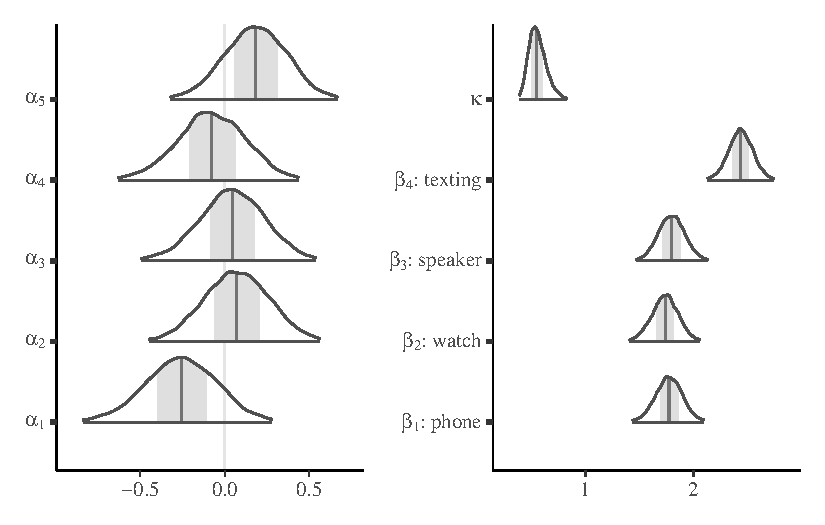
\includegraphics[keepaspectratio]{priors_files/figure-pdf/fig-post-dist-poisson-mixed-1.pdf}}

}

\caption{\label{fig-post-dist-poisson-mixed}Posterior density plots with
50\% credible intervals and median value for the random effects of the
first five individuals (left) and the fixed effects and random effect
variance (right).}

\end{figure}%

\end{example}

\section{Sensitivity analysis}\label{sensitivity-analysis}

Do priors matter? The answer to that question depends strongly on the
model, and how much information the data provides about hyperparameters.
While this question is easily answered in conjugate models (the relative
weight of hyperparameters relative to data can be derived from the
posterior parameters), it is not so simple in hierarchical models, where
the interplay between prior distributions is often more intricate. To
see the impact, one often has to rely on doing several analyses with
different values fr the prior and see the sensitivity of the conclusions
to these changes, for example by considering a vague prior or modifying
the parameters values (say halving or doubling). If the changes are
immaterial, then this provides reassurance that our analyses are robust.

\begin{example}[]\protect\hypertarget{exm-sensitivity-poisson-mixed}{}\label{exm-sensitivity-poisson-mixed}

To check the sensitivity of the conclusion, we revisit the modelling of
the \texttt{smartwatch} experiment data using a Poisson regression and
compare four priors: a uniform prior truncated to \([0, 10],\) an
inverse gamma \(\mathsf{InvGamma}(0.01, 0.01)\) prior, a penalized
complexity prior such that the 0.95 percentile of the scale is 5,
corresponding to \(\mathsf{Exp}(0.6).\) Since each distraction type
appears 31 times, there is plenty of information to reliably estimate
the dispersion \(\kappa\) of the random effects \(\alpha\): the
different density plots in Figure~\ref{fig-sensitivity} are virtually
indistinguishable from one another. This is perhaps unsurprising given
the large number of replicates, and the significant variability between
groups.

\begin{figure}[ht!]

\centering{

\pandocbounded{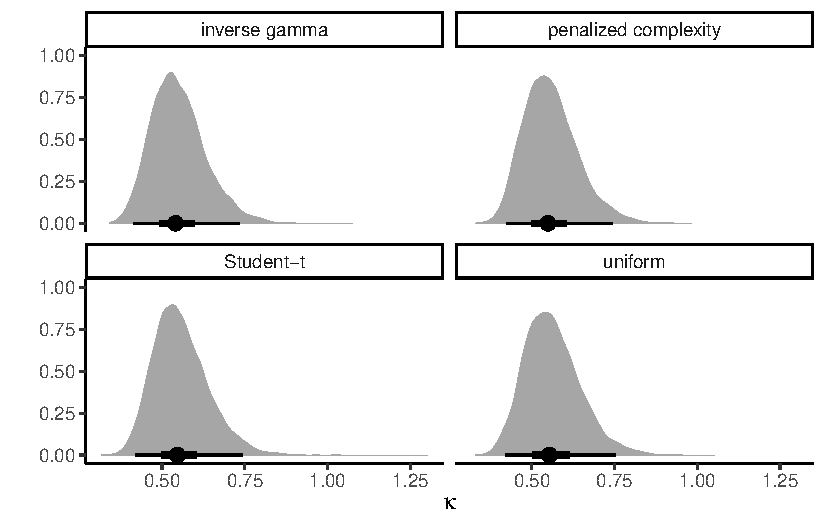
\includegraphics[keepaspectratio]{priors_files/figure-pdf/fig-sensitivity-1.pdf}}

}

\caption{\label{fig-sensitivity}Posterior density of the scale of the
random effects with uniform, inverse gamma, penalized complexity and
folded Student-t with three degrees of freedom. The circle denotes the
median and the bars the 50\% and 95\% percentile credible intervals.}

\end{figure}%

\end{example}

\begin{example}[Extreme rainfall in Abisko,
Sweden]\protect\hypertarget{exm-rainfall-abisko}{}\label{exm-rainfall-abisko}

As illustrating example, consider maximum daily cumulated rainfall in
Abisko, Sweden. The time series spans from 1913 until December 2014; we
compute the 102 yearly maximum, which range from 11mm to 62mm, and fit a
generalized extreme value distribution to these.

For the priors, suppose an expert elicits quantiles of the 10, 50 and
100 years return levels; say 30mm, 45mm and 70mm, respectively, for the
median and likewise 40mm, 70mm and 120mm for the 90\% percentile of the
return levels. We can compute the differences and calculate the
parameters of the gamma distribution through moment-matching: this gives
roughly a shape of \(\alpha_1=18.27\) and \(\beta_1=0.6,\) etc.
Figure~\ref{fig-gev-colestawn-quant-prior} shows the transfer from the
prior predictive to the posterior distribution. The prior is much more
dispersed and concentrated on the tail, which translates in a less
peaked posterior than using a weakly informative prior (dotted line):
the mode of the latter is slightly to the left and with lower density in
the tail.

\begin{figure}[ht!]

\centering{

\pandocbounded{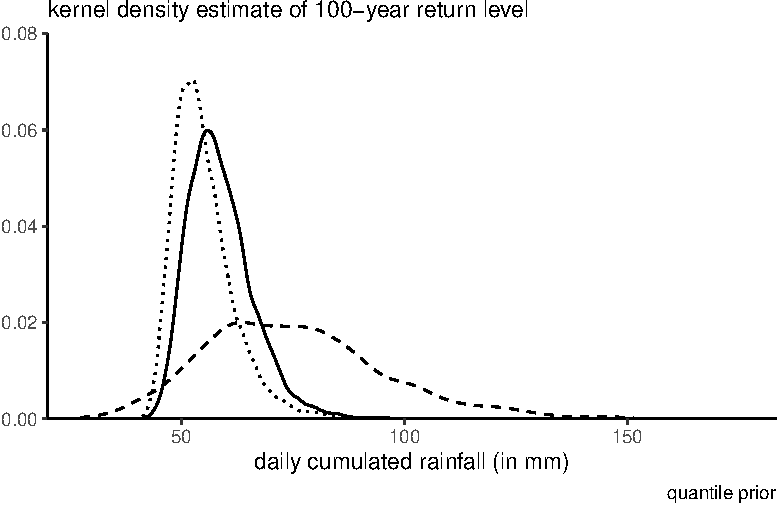
\includegraphics[keepaspectratio]{priors_files/figure-pdf/fig-gev-colestawn-quant-prior-1.pdf}}

}

\caption{\label{fig-gev-colestawn-quant-prior}Kernel density estimates
of draws from the posterior distribution of 100 year return levels with
a Coles--Tawn quantile prior (full line) and from the corresponding
prior predictive (dashed). The dotted line gives the posterior
distribution for a maximum domain information prior on the shape with
improper priors on location and scale.}

\end{figure}%

\end{example}

\begin{tcolorbox}[enhanced jigsaw, colframe=quarto-callout-important-color-frame, colback=white, leftrule=.75mm, opacitybacktitle=0.6, toprule=.15mm, colbacktitle=quarto-callout-important-color!10!white, title=\textcolor{quarto-callout-important-color}{\faExclamation}\hspace{0.5em}{\textbf{Summary}:}, left=2mm, breakable, titlerule=0mm, bottomrule=.15mm, opacityback=0, bottomtitle=1mm, rightrule=.15mm, arc=.35mm, toptitle=1mm, coltitle=black]

\begin{itemize}
\tightlist
\item
  Priors are distributions for the parameters. In multi-parameter
  models, they can be specified through a joint distribution or assumed
  independent apriori (which does not translate into independence a
  posteriori).
\item
  Priors are not invariant to reparametrization, except when they are
  constructed with this property (e.g., Jeffrey's prior or
  penalized-complexity priors).
\item
  Improper priors may lead to improper posterior.
\item
  Priors that restrict the domain of \(\boldsymbol{\theta}\) will also
  restrict the posterior. These are useful to avoid regions that are
  implausible or impossible.
\item
  Physical knowledge of the system can be helpful to specify sensible
  values of the prior through moment matching.
\item
  Conjugate priors facilitate derivations, but are mostly chosen for
  convenience.
\item
  Generally, the prior has constant weight \(\mathrm{O}(1)\), relative
  to \(\mathrm{O}(n)\) for the likelihood. The posterior is thus
  dominated in most circumstances by the likelihood.
\item
  We can compute the prior to posterior gain by comparing their density
  (if the prior is proper).
\item
  For many (conjugate) priors, we can view some function of the
  parameter as given a prior number of observations (in Gaussian models,
  binomial, gamma, etc.)
\item
  Informative priors can be used to specify expert knowledge about the
  system. This will impact the posterior, but often in a sensible
  manner, thereby regularizing or improving posterior inference.
\end{itemize}

\end{tcolorbox}

\bookmarksetup{startatroot}

\chapter{Monte Carlo methods}\label{monte-carlo-methods}

There are two major approaches to handling the problem of the unknown
normalizing constant: deterministic and stochastic approximations. The
former includes Laplace and nested Laplace approximations, variational
methods and expectation propagation. This chapter covers the latter,
stochastic approximations, and focuses on implementation of basic Markov
chain Monte Carlo algorithms. The simulation algorithms circumvent the
need to calculate the normalizing constant of the posterior entirely. We
present several examples of implementations, several tricks for tuning
and diagnostics of convergence.

We have already used Monte Carlo methods to compute posterior quantities
of interest in conjugate models. Outside of models with conjugate
priors, the lack of closed-form expression for the posterior precludes
inference. Indeed, calculating the posterior probability of an event, or
posterior moments, requires integration of the normalized posterior
density and thus knowledge of the marginal likelihood. It is seldom
possible to sample independent and identically distributed (iid) samples
from the target, especially if the model is high dimensional: rejection
sampling and the ratio of uniform method are examples of Monte Carlo
methods which can be used to generate iid draws. Ordinary Monte Carlo
methods suffer from the curse of dimensionality, with few algorithms are
generic enough to be useful in complex high-dimensional problems.
Instead, we will construct a Markov chain with a given invariant
distribution corresponding to the posterior. Markov chain Monte Carlo
methods generate correlated draws that will target the posterior under
suitable conditions.\footnote{While we won't focus on the fine prints of
  the contract, there are conditions for validity and these matter!}

\section{Monte Carlo methods}\label{monte-carlo-methods-1}

Monte Carlo methods relies on the ability to simulate random variable.
If the quantile function admits a closed-form, we can use this to
simulation. Recall that if a random variable \(X\) has distribution
function \(F,\) then we can define it's \textbf{generalized inverse}
\begin{align*}
F^{-1}(u) = \inf\{x: f(x) \geq u\}
\end{align*} and if \(G\) is continuous, then
\(F(X) \sim \mathsf{unif}(0,1).\) We can thus simulate data using the
quantile function \(F^{-1}(U),\) with \(U \sim \mathsf{unif}(0,1).\)

\begin{example}[Simulation of exponential
variates]\protect\hypertarget{exm-simulation-inverse}{}\label{exm-simulation-inverse}

The distribution function of \(Y \sim \mathsf{expo}(\lambda)\) is
\(F(y) = \exp(-\lambda y)\), so the quantile function is
\(F^{-1}(u) = -\log(u) / \lambda\)

\begin{Shaded}
\begin{Highlighting}[]
\NormalTok{n }\OtherTok{\textless{}{-}} \FloatTok{1e4}\NormalTok{L}
\SpecialCharTok{{-}}\FunctionTok{log}\NormalTok{(}\FunctionTok{runif}\NormalTok{(n)) }\SpecialCharTok{/} \DecValTok{2} \CommentTok{\#simulate expo(2)}
\end{Highlighting}
\end{Shaded}

\end{example}

\begin{theorem}[Fundamental theorem of
simulation]\protect\hypertarget{thm-fundamental-simulation}{}\label{thm-fundamental-simulation}

Consider a \(d\)-variate random vector \(\boldsymbol{X},\) independently
\(U \sim \mathsf{unif}(0,1)\) and \(c>0\) any positive constant. If
\((\boldsymbol{X}, U)\) is uniformly distributed on the set
\begin{align*}
\mathcal{A}_{f}=\{(\boldsymbol{x}, u): 0 \leq u \leq  c f(\boldsymbol{x})\},
\end{align*} then \(\boldsymbol{X}\) has density \(f(\boldsymbol{x}).\)
Conversely, if \(\boldsymbol{X}\) has density \(f(\boldsymbol{x})\) and
\(U\sim\mathsf{unif}(0,1)\) independently, then
\([\boldsymbol{X}, cUf(\boldsymbol{X})]\) is uniformly distributed on
\(\mathcal{A}_f\)

We can thus view \(f\) as the marginal density of \(\boldsymbol{X}\)
since \(f(\boldsymbol{x}) = \int_0^{f(\boldsymbol{x})} \mathrm{d} u.\)
If we can simulate uniformly from \(\mathcal{A}_{f},\) then, we can
discard the auxiliary variable \(u.\) See Devroye
(\citeproc{ref-Devroye:1986}{1986}), Theorem 3.1 for a proof.

\begin{figure}[ht!]

\centering{

\pandocbounded{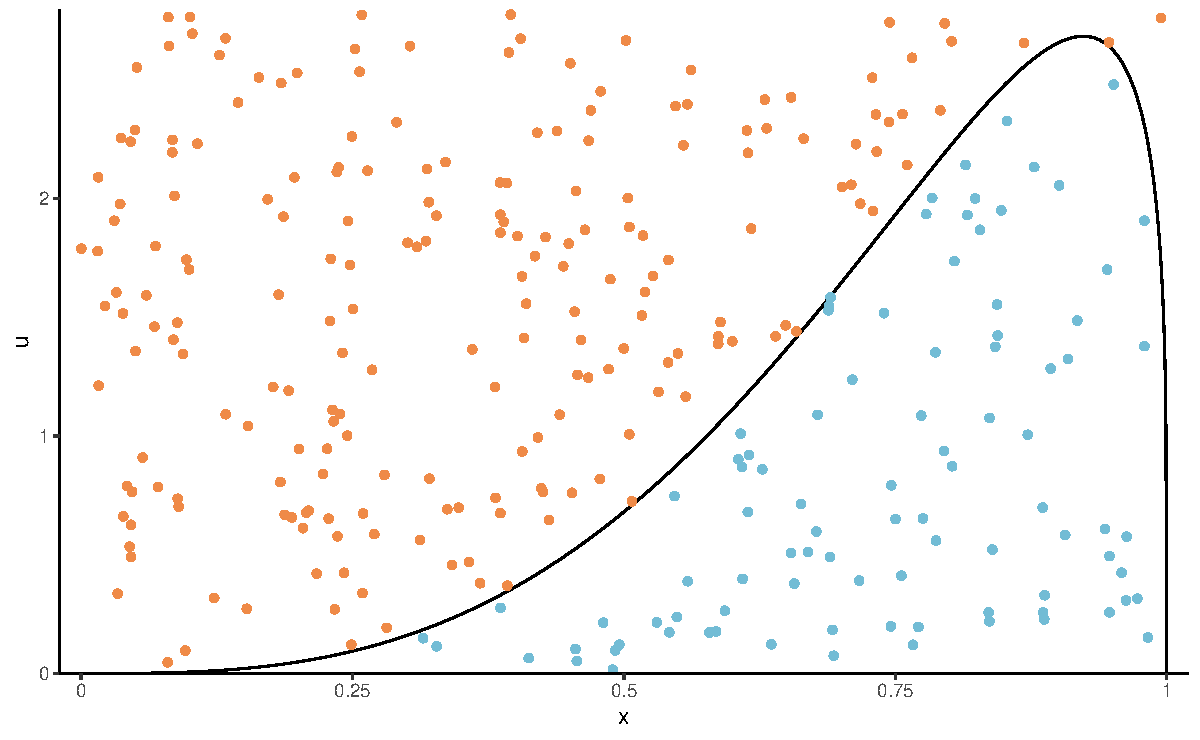
\includegraphics[keepaspectratio]{montecarlo_files/figure-pdf/fig-fundamental-theorem-1.pdf}}

}

\caption{\label{fig-fundamental-theorem}Illustration of the fundamental
theorem of simulation. All points in blue below the density curve belong
to \(\mathcal{A}_f.\)}

\end{figure}%

\end{theorem}

The fundamental theorem of simulation underlies rejection sampling, the
generalized ratio of uniform and slice sampling. The density function
needs only to be known up to normalizing constant thanks to the
arbitrariness of \(c,\) which will also allow us to work with
unnormalized density functions.

\begin{proposition}[Rejection
sampling]\protect\hypertarget{prp-rejection-sampling}{}\label{prp-rejection-sampling}

Rejection sampling (also termed accept-reject algorithm) samples from a
random vector with density \(p(\cdot)\) by drawing candidates from a
proposal with density \(q(\cdot)\) with nested support,
\(\mathrm{supp}(p) \subseteq \mathrm{supp}(q).\) The density
\(q(\cdot)\) must be such that
\(p(\boldsymbol{\theta}) \leq C q(\boldsymbol{\theta})\) for
\(C \geq 1\) for all values of \(\boldsymbol{\theta}\) in the support of
\(p(\cdot).\)

\begin{enumerate}
\def\labelenumi{\arabic{enumi}.}
\tightlist
\item
  Generate \(\boldsymbol{\theta}^{\star}\) from the proposal with
  density \(q\) and \(U \sim \mathsf{U}(0,1)\)
\item
  Compute the ratio
  \(R \gets p(\boldsymbol{\theta}^{\star})/ q(\boldsymbol{\theta}^{\star}).\)
\item
  If \(R \geq CU,\) return \(\boldsymbol{\theta},\) else go back to step
  1.
\end{enumerate}

\end{proposition}

\begin{figure}[ht!]

\centering{

\pandocbounded{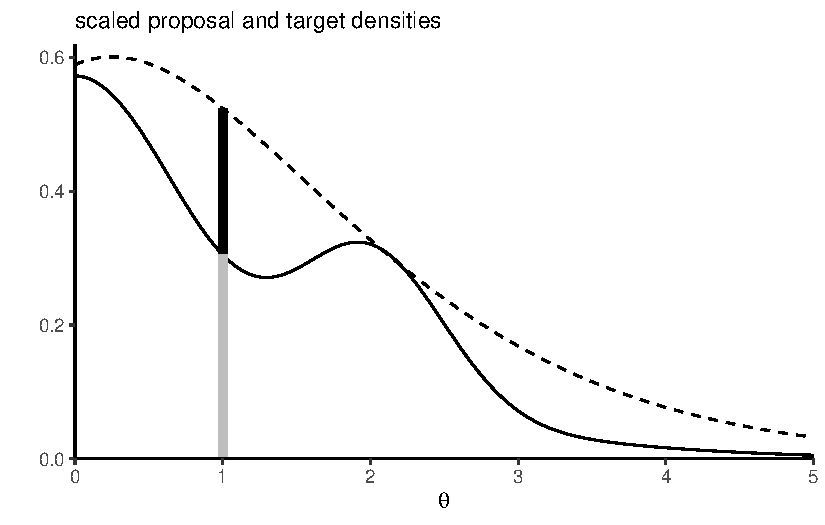
\includegraphics[keepaspectratio]{montecarlo_files/figure-pdf/fig-acceptreject-1.pdf}}

}

\caption{\label{fig-acceptreject}Target density (full) and scaled
proposal density (dashed): the vertical segment at \(\theta=1\) shows
the percentage of acceptance for a uniform slice under the scaled
proposal, giving an acceptance ratio of 0.58.}

\end{figure}%

Rejection sampling requires the proposal \(q\) to have a support at
least as large as that of \(p\) and resemble closely the density. It
should be chosen so that the upper bound \(C\) is as sharp as possible
and close to 1. The dominating density \(q\) must have heavier tails
than the density of interest. The expected number of simulations needed
to accept one proposal is \(C.\) Finally, for the method to be useful,
we need to be able to simulate easily and cheaply from the proposal. The
optimal value of \(C\) is
\(C = \sup_{\boldsymbol{\theta}} p(\boldsymbol{\theta}) / q(\boldsymbol{\theta}).\)
This quantity may be obtained by numerical optimization, by finding the
mode of the ratio of the log densities if the maximum is not known
analytically.

\begin{example}[Truncated Gaussian
distribution]\protect\hypertarget{exm-accept-reject-truncated}{}\label{exm-accept-reject-truncated}

Consider the problem of sampling from a Gaussian distribution
\(Y \sim \mathsf{Gauss}(\mu, \sigma^2)\) truncated in the interval
\([a, b],\) which has density \begin{align*}
f(x; \mu, \sigma, a, b) = \frac{1}{\sigma}\frac{\phi\left(\frac{x-\mu}{\sigma}\right)}{\Phi\{(b-\mu)/\sigma\}-\Phi\{(a-\mu)/\sigma\}}.
\end{align*} where \(\phi(\cdot), \Phi(\cdot)\) are respectively the
density and distribution function of the standard Gaussian distribution.

Since the Gaussian is a location-scale family, we can reduce the problem
to sampling \(X\) from a standard Gaussian truncated on
\(\alpha = (a-\mu)/\sigma\) and \(\beta = (b-\mu)/\sigma\) and back
transform the result as \(Y = \mu + \sigma X.\)

A crude accept-reject sampling algorithm would consider sampling from
the same untruncated distribution with density
\(g(X) = \sigma^{-1}\phi\{(x-\mu)/\sigma\},\) and the acceptance ratio
is \(C^{-1}=\{\Phi(\beta) - \Phi(\alpha)\}.\) We thus simply simulate
points from the Gaussian and accept any that falls within the bounds.

\begin{Shaded}
\begin{Highlighting}[]
\CommentTok{\# Standard Gaussian truncated on [0,1]}
\NormalTok{candidate }\OtherTok{\textless{}{-}} \FunctionTok{rnorm}\NormalTok{(}\FloatTok{1e5}\NormalTok{)}
\NormalTok{trunc\_samp }\OtherTok{\textless{}{-}}\NormalTok{ candidate[candidate }\SpecialCharTok{\textgreater{}=} \DecValTok{0} \SpecialCharTok{\&}\NormalTok{ candidate }\SpecialCharTok{\textless{}=} \DecValTok{1}\NormalTok{]}
\CommentTok{\# Acceptance rate}
\FunctionTok{length}\NormalTok{(trunc\_samp)}\SpecialCharTok{/}\FloatTok{1e5}
\end{Highlighting}
\end{Shaded}

\begin{verbatim}
[1] 0.34002
\end{verbatim}

\begin{Shaded}
\begin{Highlighting}[]
\CommentTok{\# Theoretical acceptance rate}
\FunctionTok{pnorm}\NormalTok{(}\DecValTok{1}\NormalTok{)}\SpecialCharTok{{-}}\FunctionTok{pnorm}\NormalTok{(}\DecValTok{0}\NormalTok{)}
\end{Highlighting}
\end{Shaded}

\begin{verbatim}
[1] 0.3413447
\end{verbatim}

We can of course do better: if we consider a random variable with
distribution function \(F,\) but truncated over the interval \([a,b],\)
then the resulting distribution function is
\[\frac{F(x) - F(a)}{F(b)-F(a)}, \qquad a \leq x \leq b,\] and we can
invert this expression to get the quantile function of the truncated
variable in terms of the distribution function \(F\) and the quantile
function \(F^{-1}\) of the original untruncated variable.

For the Gaussian, this gives \begin{align*}
X \sim \Phi^{-1}\left[\Phi(a) + \{\Phi(b)-\Phi(a)\}U\right]
\end{align*} for \(U \sim \mathsf{U}(0,1).\) Although the quantile and
distribution functions of the Gaussian, \texttt{pnorm} and
\texttt{qnorm} in \textbf{R}, are very accurate, this method will fail
for rare event simulation because it will return \(\Phi(x) = 0\) for
\(x \leq -39\) and \(\Phi(x)=1\) for \(x \geq 8.3,\) implying that
\(a \leq 8.3\) for this approach to work
(\citeproc{ref-LEcuyer.Botev:2017}{Botev and L'Écuyer 2017}).

Consider the problem of simulating events in the right tail for a
standard Gaussian where \(a > 0\); Marsaglia's method
(\citeproc{ref-Devroye:1986}{Devroye 1986, 381}), can be used for that
purpose. Write the density of the Gaussian as
\(f(x) = \exp(-x^2/2)/c_1,\) where
\(c_1 = \int_{a}^{\infty}\exp(-z^2/2)\mathrm{d} z,\) and note that
\[c_1f(x) \leq \frac{x}{a}\exp\left(-\frac{x^2}{2}\right)= a^{-1}\exp\left(-\frac{a^2}{2}\right)g(x), \qquad x \geq a;\]
where \(g(x)\) is the density of a Rayleigh variable shifted by \(a,\)
which has distribution function \(G(x) = 1-\exp\{(a^2-x^2)/2\}\) for
\(x \geq a.\) We can simulate such a random variate \(X\) through the
inversion method. The constant \(C= \exp(-a^2/2)(c_1a)^{-1}\) approaches
1 quickly as \(a \to \infty.\)

The accept-reject thus proceeds with

\begin{enumerate}
\def\labelenumi{\arabic{enumi}.}
\tightlist
\item
  Generate a shifted Rayleigh above \(a,\)
  \(X \gets  \{a^2 - 2\log(U)\}^{1/2}\) for \(U \sim \mathsf{U}(0,1)\)
\item
  Accept \(X\) if \(XV \leq a,\) where \(V \sim \mathsf{U}(0,1).\)
\end{enumerate}

Should we wish to obtain samples on \([a,b],\) we could instead propose
from a Rayleigh truncated above at \(b\)
(\citeproc{ref-LEcuyer.Botev:2017}{Botev and L'Écuyer 2017}).

\begin{Shaded}
\begin{Highlighting}[]
\NormalTok{a }\OtherTok{\textless{}{-}} \FloatTok{8.3}
\NormalTok{niter }\OtherTok{\textless{}{-}} \DecValTok{1000}\NormalTok{L}
\NormalTok{X }\OtherTok{\textless{}{-}} \FunctionTok{sqrt}\NormalTok{(a}\SpecialCharTok{\^{}}\DecValTok{2} \SpecialCharTok{+} \DecValTok{2}\SpecialCharTok{*}\FunctionTok{rexp}\NormalTok{(niter))}
\NormalTok{samp }\OtherTok{\textless{}{-}}\NormalTok{ X[}\FunctionTok{runif}\NormalTok{(niter)}\SpecialCharTok{*}\NormalTok{X }\SpecialCharTok{\textless{}=}\NormalTok{ a]}
\end{Highlighting}
\end{Shaded}

\end{example}

For a given candidate density \(g\) which has a heavier tail than the
target, we can resort to numerical methods to compute the mode of the
ratio \(f/g\) and obtain the bound \(C\); see Albert
(\citeproc{ref-Albert:2009}{2009}), Section 5.8 for an insightful
example. A different use for the simulations is to approximate integrals
numerically. Consider a target distribution with finite expected value.
The law of large numbers guarantees that, if we can draw observations
from our target distribution, then the sample average will converge to
the expected value of that distribution, as the sample size becomes
larger and larger, provided the expectation is finite. We can thus
compute the probability of any event or the expected value of any
(integrable) function by computing sample averages; the cost to pay for
this generality is randomness.

\begin{proposition}[Generalized
ratio-of-uniform]\protect\hypertarget{prp-ratio-uniform}{}\label{prp-ratio-uniform}

An exact simulation algorithm is described in Kinderman and Monahan
(\citeproc{ref-Kinderman.Monahan:1977}{1977}) and extended Wakefield,
Gelfand, and Smith (\citeproc{ref-Wakefield.Gelfand.Smith:1991}{1991})
for random number generation in low dimensions. Consider a \(d\)-vector
\(\boldsymbol{X}\) with density
\(cf(\boldsymbol{x}): \mathbb{R}^d \to \mathbb{R}^{+}\) with support
\(\mathcal{S} \subseteq \mathbb{R}^d\), and \(c>0\) is the (possibly
unknown) normalizing constant. Consider variables
\(\boldsymbol{u} = (u_0, u_1, \ldots, u_d)\) uniformly distributed over
the set \begin{align*}
\mathcal{B}(r) = \left\{ (u_0, u_1, \ldots, u_d) \in \mathbb{R}^{d+1}: 0 < u_0 \leq \left[ f\left( \frac{u_1}{u_0^r}, \ldots, \frac{u_d}{u_0^r} \right) \right] ^ {1/(r d + 1)} \right\}
\end{align*} for some positive radius parameter \(r \geq 0\). The
measure of the set \(\mathcal{B}(r)=c^{-1}(1+rd)^{-1}.\) By
Theorem~\ref{thm-fundamental-simulation},
\((u_1 / u_0^r, \ldots, u_d / u_0^r)\) is drawn from the renormalized
density \(cf(x)\). The challenge lies in simulating \(\boldsymbol{u}\)
uniformly over \(\mathcal{B}_r\), but we can use accept-reject if the
later is enclosed in a bounding box \(\mathbb{B}\), keeping only samples
that satisfy the constraints. If, over \(\mathcal{S}\),
\(f(\boldsymbol{x})\) and \(x_i^{r d +1} f(\boldsymbol{x})^r\) for
\(i = 1, \ldots, d\) are bounded then we can enclose \(\mathcal{B}(r)\)
within the \((d+1)\)-dimensional bounding box
\[\mathbb{B}=\{a_j(r) \leq u_i \leq b_j(r);  j = 0, \ldots, d \},\] with
\(a_0(r)=0\). The parameters of the bounding box are\\
\begin{align*}
b_0(r) &= \sup_{\boldsymbol{x} \in \mathcal{S}} \, f(\boldsymbol{x})^{1 / (r d + 1)}, \\
a_j(r) &= \inf_{\substack{\boldsymbol{x} \in \mathcal{S}\\ x_i \leq 0}} \, x_i \, f(\boldsymbol{x})^{r / (r d + 1)}, \\  
b_j(r) &= \sup_{{\substack{\boldsymbol{x} \in \mathcal{S}\\ x_i \geq 0}}} \, x_i \, f(\boldsymbol{x})^{r / (r d + 1)},  
\end{align*}

The probability of acceptance \(p_a(d, r)\) of a point simulated
uniformly over the bounding box depends on both the radius and the
dimension and is \begin{align*}
p_a(d, r) = c\left[(r d + 1) \, b_0(r) \displaystyle\prod_{j=1}^d \left\{b_j(r) -a_j(r) \right\}\right]^{-1}.
\end{align*}

Wakefield, Gelfand, and Smith
(\citeproc{ref-Wakefield.Gelfand.Smith:1991}{1991}) propose using
\(r=1/2\) and relocating the mode of \(f\) to the origin increase the
acceptance rate. Northrop proposes to use a Box--Cox transformation
(\citeproc{ref-Box.Cox:1964}{Box and Cox 1964}) together with a rotation
in the software Northrop (\citeproc{ref-rust}{2024}) to improve the
acceptance rate. The bounding box may exist only for certain values of
\(r\); see the
\href{https://paulnorthrop.github.io/rust/articles/rust-a-vignette.html}{\texttt{rust}
package vignette} for technical details and examples.

\end{proposition}

\begin{example}[Ratio-of-uniform for insurance
loss]\protect\hypertarget{exm-rust}{}\label{exm-rust}

We use the ratio-of-uniform algorithm presented in
Proposition~\ref{prp-ratio-uniform} for the data from
Example~\ref{exm-loss-extremes} to generate draws from the posterior. We
illustrate below the \texttt{rust} package with a user-specified prior
and posterior. We fit a generalized Pareto distribution
\(Y \sim \mathsf{gen. Pareto}(\tau, \xi)\) to exceedances above 10
millions krones to the \texttt{danish} fire insurance data, using a
truncated maximal data information prior
\(p(\tau, \xi) \propto \tau^{-1}\exp(-\xi+1)\mathrm{I}(\xi > -1).\)

\begin{Shaded}
\begin{Highlighting}[]
\FunctionTok{data}\NormalTok{(danish, }\AttributeTok{package =} \StringTok{"evir"}\NormalTok{)}
\CommentTok{\# Extract threshold exceedances}
\NormalTok{exc }\OtherTok{\textless{}{-}}\NormalTok{ danish[danish }\SpecialCharTok{\textgreater{}} \DecValTok{10}\NormalTok{] }\SpecialCharTok{{-}} \DecValTok{10}
\CommentTok{\# Create a function for the log prior}
\NormalTok{logmdiprior }\OtherTok{\textless{}{-}} \ControlFlowTok{function}\NormalTok{(par, ...)\{}
  \ControlFlowTok{if}\NormalTok{(}\FunctionTok{isTRUE}\NormalTok{(}\FunctionTok{any}\NormalTok{(par[}\DecValTok{1}\NormalTok{] }\SpecialCharTok{\textless{}=} \DecValTok{0}\NormalTok{, par[}\DecValTok{2}\NormalTok{] }\SpecialCharTok{\textless{}} \SpecialCharTok{{-}}\DecValTok{1}\NormalTok{)))\{}
    \FunctionTok{return}\NormalTok{(}\SpecialCharTok{{-}}\ConstantTok{Inf}\NormalTok{)}
\NormalTok{  \}}
  \SpecialCharTok{{-}}\FunctionTok{log}\NormalTok{(par[}\DecValTok{1}\NormalTok{]) }\SpecialCharTok{{-}}\NormalTok{ par[}\DecValTok{2}\NormalTok{]}
\NormalTok{\}}
\CommentTok{\# Same for log likelihood, assuming independent data}
\NormalTok{loglik\_gp }\OtherTok{\textless{}{-}} \ControlFlowTok{function}\NormalTok{(par, }\AttributeTok{data =}\NormalTok{ exc, ...)\{}
  \ControlFlowTok{if}\NormalTok{(}\FunctionTok{isTRUE}\NormalTok{(}\FunctionTok{any}\NormalTok{(par[}\DecValTok{1}\NormalTok{] }\SpecialCharTok{\textless{}=} \DecValTok{0}\NormalTok{, par[}\DecValTok{2}\NormalTok{] }\SpecialCharTok{\textless{}} \SpecialCharTok{{-}}\DecValTok{1}\NormalTok{)))\{}
    \FunctionTok{return}\NormalTok{(}\SpecialCharTok{{-}}\ConstantTok{Inf}\NormalTok{)}
\NormalTok{  \}}
  \FunctionTok{sum}\NormalTok{(mev}\SpecialCharTok{::}\FunctionTok{dgp}\NormalTok{(}\AttributeTok{x =}\NormalTok{ data, }\AttributeTok{scale =}\NormalTok{ par[}\DecValTok{1}\NormalTok{], }\AttributeTok{shape =}\NormalTok{ par[}\DecValTok{2}\NormalTok{], }\AttributeTok{log =} \ConstantTok{TRUE}\NormalTok{))}
\NormalTok{\}}
\NormalTok{logpost }\OtherTok{\textless{}{-}} \ControlFlowTok{function}\NormalTok{(par, ...)\{}
  \FunctionTok{logmdiprior}\NormalTok{(par) }\SpecialCharTok{+} \FunctionTok{loglik\_gp}\NormalTok{(par)}
\NormalTok{\}}
\CommentTok{\# Sampler using ratio{-}of{-}uniform method}
\NormalTok{ru\_output }\OtherTok{\textless{}{-}}\NormalTok{ rust}\SpecialCharTok{::}\FunctionTok{ru}\NormalTok{(}
  \AttributeTok{logf =}\NormalTok{ logpost,  }\CommentTok{\# log posterior function}
  \AttributeTok{n =} \DecValTok{10000}\NormalTok{, }\CommentTok{\# number of posterior draws}
  \AttributeTok{d =} \DecValTok{2}\NormalTok{, }\CommentTok{\# dimension of the parameter vector}
  \AttributeTok{init =}\NormalTok{ mev}\SpecialCharTok{::}\FunctionTok{fit.gpd}\NormalTok{(danish, }\AttributeTok{thresh =} \DecValTok{10}\NormalTok{)}\SpecialCharTok{$}\NormalTok{par, }\CommentTok{\#mle}
  \AttributeTok{lower =} \FunctionTok{c}\NormalTok{(}\DecValTok{0}\NormalTok{, }\SpecialCharTok{{-}}\DecValTok{1}\NormalTok{))}
\DocumentationTok{\#\# Acceptance rate }
\CommentTok{\# ru\_output$pa}
\DocumentationTok{\#\# Posterior samples}
\NormalTok{postsamp }\OtherTok{\textless{}{-}}\NormalTok{ ru\_output}\SpecialCharTok{$}\NormalTok{sim\_vals}
\end{Highlighting}
\end{Shaded}

Even without modification, the acceptance rate is 52\%, which is quite
efficient in the context. The generalized Pareto approximation suggests
a very heavy tail: values of \(\xi \geq 1\) correspond to distributions
with infinite first moment, and those with \(\xi \geq 1/2\) to infinite
variance.

\begin{figure}[ht!]

\centering{

\pandocbounded{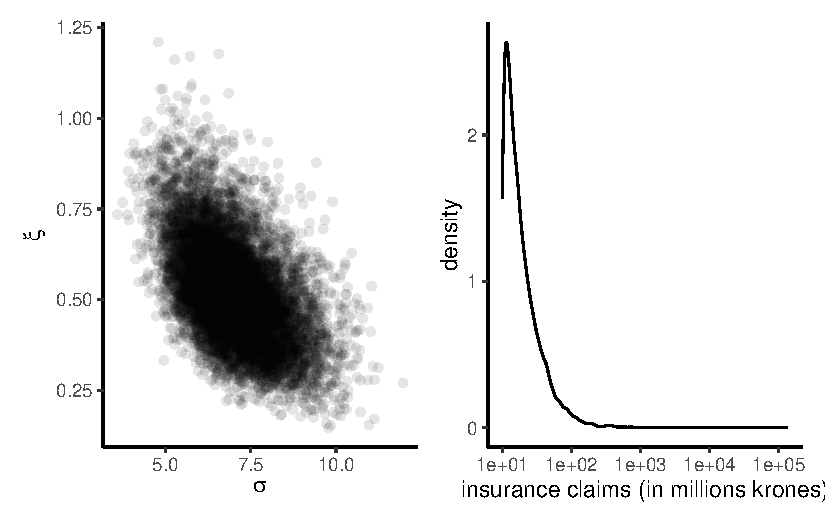
\includegraphics[keepaspectratio]{montecarlo_files/figure-pdf/fig-danish-rou-1.pdf}}

}

\caption{\label{fig-danish-rou}Scatterplot of posterior samples from the
generalized Pareto model applied to Danish fire insurance losses above
10 millions krones, with maximal data information prior (left) and
posterior predictive density on log scale (right).}

\end{figure}%

\end{example}

\begin{proposition}[Monte Carlo
integration]\protect\hypertarget{prp-monte-carlo-integration}{}\label{prp-monte-carlo-integration}

Specifically, suppose we are interested in the average
\(\mathsf{E}\{g(X)\}\) of \(X\) with density or mass function \(f\)
supported on \(\mathcal{X}\) for some function \(g.\) Monte Carlo
integration proceeds by drawing \(B\) independent samples
\(x_1, \ldots, x_B\) from density \(p\) and evaluating the empirical
average of \(g,\) with \begin{align*}
\mathsf{E}\{g(X)\} = \int_{\mathcal{X}} g(x) p(x) \mathrm{d} x \approx \widehat{\mathsf{E}}\{g(X)\}=\frac{1}{B}\sum_{b=1}^B g(x_b).
\end{align*} By the law of large number, this estimator is convergent
when \(B \to \infty\) provided that the expectation is finite. If the
variance of \(g(X)\) is finite, we can approximate the latter by the
sample variance of the simple random sample and obtain the Monte Carlo
standard error of the estimator \begin{align*}
\mathsf{se}^2[\widehat{\mathsf{E}}\{g(X)\}] = \frac{1}{B(B-1)} \sum_{b=1}^B \left[ g(x_b) -  \widehat{\mathsf{E}}\{g(X)\} \right]^2.
\end{align*}

\end{proposition}

We can also use a similar idea to evaluate the integral of \(g(X)\) if
\(X\) has density \(p,\) by drawing instead samples from \(q.\) This is
formalized in the next proposition.

\begin{proposition}[Importance
sampling]\protect\hypertarget{prp-importance-sampling}{}\label{prp-importance-sampling}

Consider a random variable \(X\) with density \(p(x)\) supported on
\(\mathcal{X}.\) We can calculate the integral
\(\mathsf{E}_p\{g(X)\} = \int_{\mathcal{X}} g(x) p(x) \mathrm{d}x\) by
considering instead draws from a density \(q(\cdot)\) with nested
support, \(\mathcal{X} \subseteq \mathrm{supp}(q).\) Then,
\begin{align*}
\mathsf{E}\{g(X)\} = \int_{\mathcal{X}} g(x) \frac{p(x)}{q(x)} q(x) \mathrm{d} x
\end{align*} and we can proceed similarly by drawing samples from \(q.\)
This is most useful when the variance is finite, which happens if the
integral \begin{align*}
\int_{\mathcal{X}} g^2(x) \frac{p^2(x)}{q(x)} \mathrm{d} x < \infty.
\end{align*} An alternative Monte Carlo estimator, which is biased but
has lower variance, is obtained by drawing independent
\(x_1, \ldots, x_B\) from \(q\) and taking instead the weighted average
of \begin{align*}
\widetilde{\mathsf{E}}\{g(X)\} =\frac{B^{-1} \sum_{b=1}^B w_b g(x_b) }{B^{-1}\sum_{b=1}^B w_b}.
\end{align*} with weights \(w_b = p(x_b)/q(x_b).\) The latter equal 1 on
average, so one could omit the denominator without harm. The standard
error for the independent draws equals \begin{align*}
\mathsf{se}^2[\widetilde{\mathsf{E}}\{g(X)\}] = \frac{ \sum_{b=1}^B w_b^2 \left[ g(x_b) -  \widetilde{\mathsf{E}}\{g(X)\} \right]^2}{\left(\sum_{b=1}^B w_b\right)^2}.
\end{align*}

\end{proposition}

\begin{example}[Importance sampling for the variance of a beta
distribution]\protect\hypertarget{exm-is-beta-variance}{}\label{exm-is-beta-variance}

Consider \(X \sim \mathsf{beta}(\alpha, \alpha)\) for \(\alpha > 1\)
with \(\mathsf{E}(X)=0.5\) since the density is symmetric. We tackle the
estimation of the variance, which can be written as
\(\mathsf{E}\{(X - 0.5)^2\}.\) While we can easily derive the
theoretical expression, equal to
\(\mathsf{Va}(X) = \{4 \cdot (2\alpha+1)\}^{-1},\) we can also use Monte
Carlo integration as proof of concept.

Rather than simulate directly from our data generating mechanism, we can
use an importance sampling density \(q(x)\) which puts more mass away
from \(0.5\) where the integral is zero. Consider the equiweighted
mixture of \(\mathsf{beta}(\alpha, 3\alpha)\) and
\(\mathsf{\beta}(3\alpha, \alpha)\), which is bimodal.
Figure~\ref{fig-importance-sampling-beta} shows the function we wish to
integrate, the density and the importance sampling density, and the
weighting function \(p(x)/q(x)\) of the first 50 observations drawn from
\(q(x)\) with \(\alpha=1.5.\) The variance ratio shows an improvement of
more than 9\% for the same Monte Carlo sample size.

\begin{Shaded}
\begin{Highlighting}[]
\NormalTok{B }\OtherTok{\textless{}{-}} \FloatTok{2e4}\NormalTok{L}
\NormalTok{alpha }\OtherTok{\textless{}{-}} \FloatTok{1.5}
\NormalTok{factor }\OtherTok{\textless{}{-}} \DecValTok{3}
\CommentTok{\# Mode at the mean 0.5}
\NormalTok{X0 }\OtherTok{\textless{}{-}} \FunctionTok{rbeta}\NormalTok{(}\AttributeTok{n =}\NormalTok{ B, alpha, alpha)}
\NormalTok{px }\OtherTok{\textless{}{-}} \ControlFlowTok{function}\NormalTok{(x)\{}\FunctionTok{dbeta}\NormalTok{(x, alpha, alpha)\}}
\CommentTok{\# Importance sampling density {-} mixture of two betas (alpha, factor*alpha)}
\NormalTok{X1 }\OtherTok{\textless{}{-}} \FunctionTok{ifelse}\NormalTok{(}\FunctionTok{runif}\NormalTok{(B) }\SpecialCharTok{\textless{}} \FloatTok{0.5}\NormalTok{, }\FunctionTok{rbeta}\NormalTok{(B, alpha, factor}\SpecialCharTok{*}\NormalTok{alpha), }\FunctionTok{rbeta}\NormalTok{(B, factor}\SpecialCharTok{*}\NormalTok{alpha, alpha))}
\NormalTok{qx }\OtherTok{\textless{}{-}} \ControlFlowTok{function}\NormalTok{(x)\{}\FloatTok{0.5}\SpecialCharTok{*}\FunctionTok{dbeta}\NormalTok{(x, alpha, factor}\SpecialCharTok{*}\NormalTok{alpha) }\SpecialCharTok{+} \FloatTok{0.5}\SpecialCharTok{*}\FunctionTok{dbeta}\NormalTok{(x, factor}\SpecialCharTok{*}\NormalTok{alpha, alpha)\}}
\CommentTok{\# Function to integrate {-} gives variance of a symmetric beta distribution}
\NormalTok{g }\OtherTok{\textless{}{-}} \ControlFlowTok{function}\NormalTok{(x)\{(x }\SpecialCharTok{{-}} \FloatTok{0.5}\NormalTok{)}\SpecialCharTok{\^{}}\DecValTok{2}\NormalTok{\}}
\CommentTok{\# Weights for importance sampling}
\NormalTok{w }\OtherTok{\textless{}{-}} \FunctionTok{px}\NormalTok{(X1)}\SpecialCharTok{/}\FunctionTok{qx}\NormalTok{(X1)}
\CommentTok{\# Monte Carlo integration}
\NormalTok{mc\_est }\OtherTok{\textless{}{-}} \FunctionTok{mean}\NormalTok{(}\FunctionTok{g}\NormalTok{(X0))}
\NormalTok{mc\_var }\OtherTok{\textless{}{-}} \FunctionTok{var}\NormalTok{(}\FunctionTok{g}\NormalTok{(X0))}\SpecialCharTok{/}\NormalTok{B}
\CommentTok{\# Importance sampling weighted mean and variance}
\NormalTok{is\_est }\OtherTok{\textless{}{-}} \FunctionTok{weighted.mean}\NormalTok{(}\FunctionTok{g}\NormalTok{(X1), }\AttributeTok{w =}\NormalTok{ w) }\CommentTok{\# equivalent to mean(g(X1)*w)/mean(w)}
\NormalTok{is\_var }\OtherTok{\textless{}{-}} \FunctionTok{sum}\NormalTok{(w}\SpecialCharTok{\^{}}\DecValTok{2}\SpecialCharTok{*}\NormalTok{(}\FunctionTok{g}\NormalTok{(X1) }\SpecialCharTok{{-}}\NormalTok{ is\_est)}\SpecialCharTok{\^{}}\DecValTok{2}\NormalTok{)}\SpecialCharTok{/}\NormalTok{ (}\FunctionTok{sum}\NormalTok{(w)}\SpecialCharTok{\^{}}\DecValTok{2}\NormalTok{)}
\CommentTok{\# True value for the beta variance}
\NormalTok{th\_est }\OtherTok{\textless{}{-}} \DecValTok{1}\SpecialCharTok{/}\NormalTok{(}\DecValTok{4}\SpecialCharTok{*}\NormalTok{(}\DecValTok{2}\SpecialCharTok{*}\NormalTok{alpha}\SpecialCharTok{+}\DecValTok{1}\NormalTok{))}
\CommentTok{\# Point estimates and differences}
\FunctionTok{round}\NormalTok{(}\FunctionTok{c}\NormalTok{(}\AttributeTok{true =}\NormalTok{ th\_est, }\StringTok{"monte carlo"} \OtherTok{=}\NormalTok{ mc\_est, }\StringTok{"importance sampling"} \OtherTok{=}\NormalTok{ is\_est),}\DecValTok{4}\NormalTok{)}
\end{Highlighting}
\end{Shaded}

\begin{verbatim}
               true         monte carlo importance sampling 
             0.0625              0.0622              0.0627 
\end{verbatim}

\begin{Shaded}
\begin{Highlighting}[]
\CommentTok{\# Ratio of std. errors for means}
\NormalTok{mc\_var}\SpecialCharTok{/}\NormalTok{is\_var }\CommentTok{\# value \textgreater{} 1 means that IS is more efficient}
\end{Highlighting}
\end{Shaded}

\begin{verbatim}
[1] 1.087118
\end{verbatim}

\begin{figure}[ht!]

\centering{

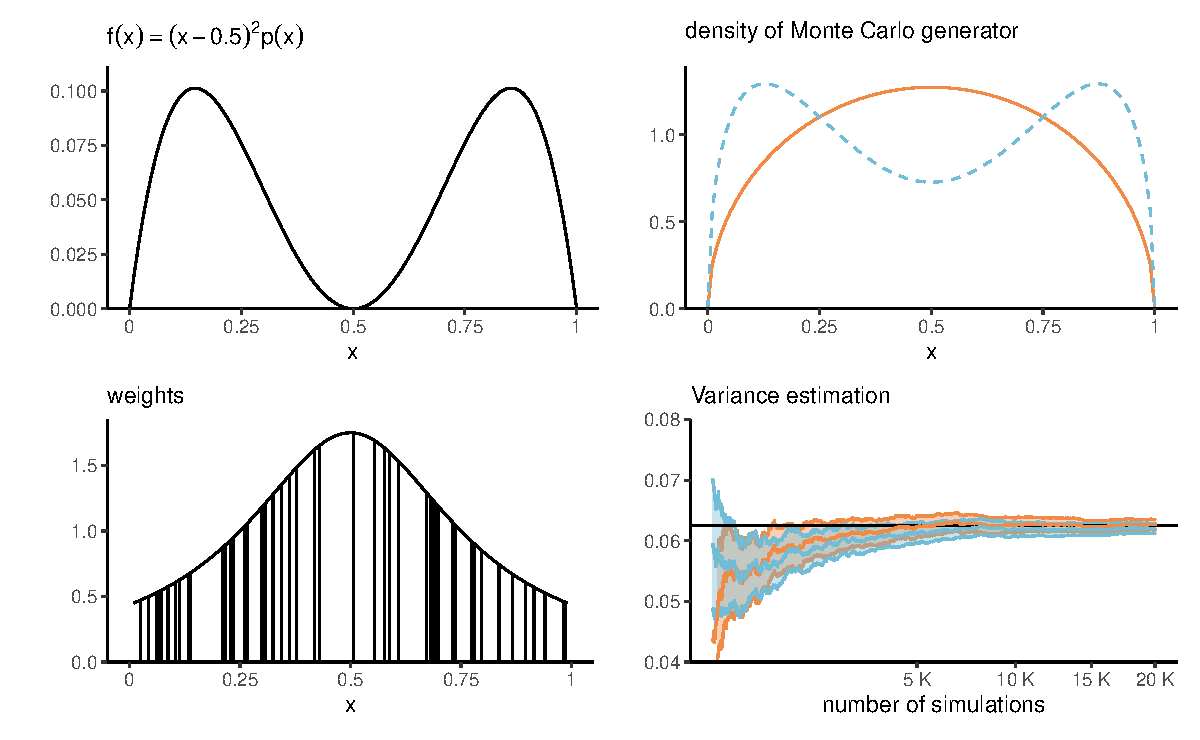
\includegraphics[width=0.95\linewidth,height=\textheight,keepaspectratio]{montecarlo_files/figure-pdf/fig-importance-sampling-beta-1.pdf}

}

\caption{\label{fig-importance-sampling-beta}Monte Carlo integration
with importance sampling for the variance of a symmetric beta
distribution. Top left: variance function \(f(x) = (x-0.5)^2\). Top
right: density of \(\mathsf{beta}(\alpha, \alpha)\) (orange) and
importance sampling mixture distribution (blue). Bottom left: weighting
function and weights for 50 first importance sampling draws. Bottom
right: sample paths of Monte Carlo mean with Wald 95\% confidence
intervals.}

\end{figure}%

\end{example}

\begin{example}[Expectations of functions of a gamma
variate]\protect\hypertarget{exm-expectation-demo}{}\label{exm-expectation-demo}

Consider \(X \sim \mathsf{gamma}(\alpha, \beta),\) a gamma distribution
with shape \(\alpha\) and rate \(\beta.\) We can compute the probability
that \(X < 1\) easily by Monte Carlo since
\(\Pr(X <1) = \mathsf{E}\{\mathrm{I}(X<1)\}\) and this means we only
need to compute the proportion of draws less than one. We can likewise
compute the mean \(g(x) = x\) or the variance as
\(\mathsf{E}(X^2) - \{\mathsf{E}(X)\}^2.\)

Suppose we have drawn a Monte Carlo sample of size \(B.\) If the
function \(g(\cdot)\) is square integrable,\footnote{Meaning
  \(\mathsf{E}\{g^2(X)\}<\infty,\) so the variance of \(g(X)\) exists.}
with variance \(\sigma^2_g,\) then a central limit theorem applies. In
large samples and for independent observations, our Monte Carlo average
\(\widehat{\mu}_g = B^{-1}\sum_{b=1}^B g(X_i)\) has variance
\(\sigma^2_g/B.\) We can approximate the unknown variance \(\sigma^2_g\)
by it's empirical counterpart.\footnote{By contrasts, if data are
  identically distributed but not independent, more care is needed.}.
Note that, while the variance decreases linearly with \(B,\) the choice
of \(g\) impacts the speed of convergence: for our examples, we can
compute \[\sigma^2_g =\Pr(X \leq 1)\{1-\Pr(X \leq 1)\}=0.0434\] (left)
and \(\sigma^2_g=\alpha/\beta^2=1/8\) (middle plot).

Figure~\ref{fig-monte-carlo-path} shows the empirical trace plot of the
Monte Carlo average (note the \(\sqrt{B}\) \(x\)-axis scale!) as a
function of the Monte Carlo sample size \(B\) along with 95\% Wald-based
confidence intervals (gray shaded region),
\(\widehat{\mu}_g \pm 1.96 \times \sigma_g/\sqrt{B}.\) We can see that
the `likely region' for the average shrinks with \(B.\)

What happens if our function is not integrable? The right-hand plot of
Figure~\ref{fig-monte-carlo-path} shows empirical averages of
\(g(x) = x^{-1},\) which is not integrable if \(\alpha < 1.\) We can
compute the empirical average, but the result won't converge to any
meaningful quantity regardless of the sample size. The large jumps are
testimonial of this.

\begin{figure}[ht!]

\centering{

\pandocbounded{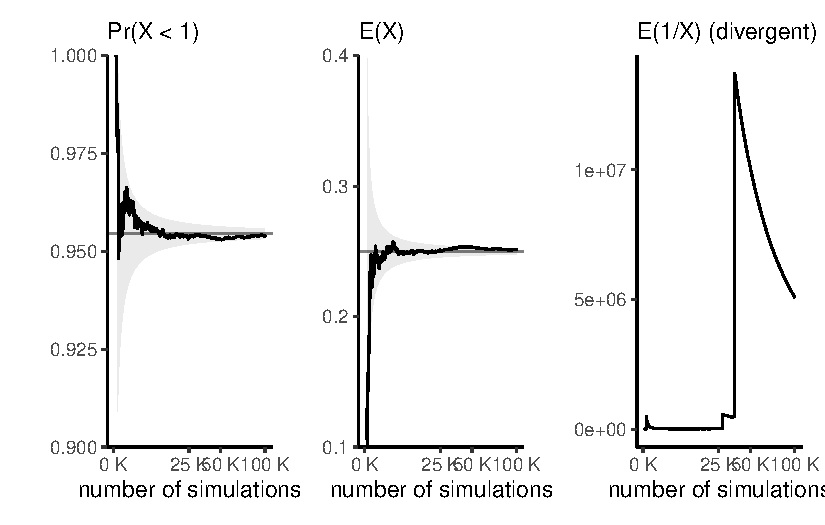
\includegraphics[keepaspectratio]{montecarlo_files/figure-pdf/fig-monte-carlo-path-1.pdf}}

}

\caption{\label{fig-monte-carlo-path}Running mean trace plots for
\(g(x)=\mathrm{I}(x<1)\) (left), \(g(x)=x\) (middle) and \(g(x)=1/x\)
(right) for a Gamma distribution with shape 0.5 and rate 2, as a
function of the Monte Carlo sample size.}

\end{figure}%

\end{example}

\begin{example}[Tail probability of a Gaussian
distribution]\protect\hypertarget{exm-tail-probability}{}\label{exm-tail-probability}

Consider estimation of the probability that a standard Gaussian random
variable exceeds \(a=4,\) which is \(p=1-\Phi(a).\) We can use standard
numerical approximations to the distribution function implemented in any
software package, which shows this probability is roughly one in
\(\ensuremath{3.1574\times 10^{4}}.\)

If we consider a truncated Gaussian above \(a,\) then the integral of
\(\mathsf{I}(x>a)\) is one (since the truncated Gaussian is a valid
density). Thus, we can estimate rather the normalizing constant by
simulating standard Gaussian and comparing this with the importance
sampling estimator, using the knowledge of the value of the integral to
derive rather the normalizing constant. Monte Carlo integration from
with \(B=10^6\) is demonstrated using the following code

\begin{Shaded}
\begin{Highlighting}[]
\NormalTok{a }\OtherTok{\textless{}{-}} \DecValTok{4}
\NormalTok{B }\OtherTok{\textless{}{-}} \FloatTok{1e6}\NormalTok{L }\CommentTok{\# 1 million draws}
\NormalTok{exact }\OtherTok{\textless{}{-}} \FunctionTok{pnorm}\NormalTok{(a, }\AttributeTok{lower.tail =} \ConstantTok{FALSE}\NormalTok{)}
\CommentTok{\# Vanilla Monte Carlo}
\NormalTok{X }\OtherTok{\textless{}{-}} \FunctionTok{rnorm}\NormalTok{(B)}
\NormalTok{mc }\OtherTok{\textless{}{-}} \FunctionTok{mean}\NormalTok{(X }\SpecialCharTok{\textgreater{}=}\NormalTok{ a)}

\CommentTok{\# Importance sampling with Rayleigh}
\NormalTok{Y }\OtherTok{\textless{}{-}} \FunctionTok{sqrt}\NormalTok{(a}\SpecialCharTok{\^{}}\DecValTok{2} \SpecialCharTok{+} \DecValTok{2}\SpecialCharTok{*}\FunctionTok{rexp}\NormalTok{(B))}
\NormalTok{drayleigh }\OtherTok{\textless{}{-}} \ControlFlowTok{function}\NormalTok{(x, a)\{ x}\SpecialCharTok{*}\FunctionTok{exp}\NormalTok{((a}\SpecialCharTok{\^{}}\DecValTok{2}\SpecialCharTok{{-}}\NormalTok{x}\SpecialCharTok{\^{}}\DecValTok{2}\NormalTok{)}\SpecialCharTok{/}\DecValTok{2}\NormalTok{)\}}
\NormalTok{is }\OtherTok{\textless{}{-}} \FunctionTok{mean}\NormalTok{(}\FunctionTok{dnorm}\NormalTok{(Y)}\SpecialCharTok{/}\FunctionTok{drayleigh}\NormalTok{(Y, }\AttributeTok{a =}\NormalTok{ a))}
\CommentTok{\# Relative error}
\FunctionTok{c}\NormalTok{(}\AttributeTok{mc =}\NormalTok{ (mc }\SpecialCharTok{{-}}\NormalTok{ exact)}\SpecialCharTok{/}\NormalTok{exact, }\AttributeTok{is =}\NormalTok{ (is }\SpecialCharTok{{-}}\NormalTok{ exact)}\SpecialCharTok{/}\NormalTok{exact)}
\end{Highlighting}
\end{Shaded}

\begin{verbatim}
           mc            is 
-2.119405e-02 -2.927613e-05 
\end{verbatim}

\end{example}

\section{Markov chains}\label{markov-chains}

Before going forward with algorithms for sampling, we introduce some
terminology that should be familiar to people with a background in time
series analysis. The treatment of Markov chains in this chapter is
rather loose and non-formal. Readers can refer to Chapter 6 of Robert
and Casella (\citeproc{ref-Casella.Robert:2004}{2004}) for a more
rigourous exposition.

\begin{definition}[Discrete-time stochastic
process]\protect\hypertarget{def-stoch-proc}{}\label{def-stoch-proc}

A discrete-time stochastic process is a random sequences whose elements
are part of some set (finite or countable), termed state space
\(\mathcal{S}.\) We can encode the probability of moving from one state
to the next via a transition matrix, whose rows contain the
probabilities of moving from one state to the next and thus sum to one.

\end{definition}

\begin{definition}[Stationarity]\protect\hypertarget{def-weak-stationarity}{}\label{def-weak-stationarity}

A stochastic (i.e., random) process is (strongly) stationary if the
distribution of \(\{X_1, \ldots, X_n\}\) is the same as that of
\(\{X_{t+1}, \ldots X_{n+t}\}\) for any value of \(t\) and given \(n.\)

It is weakly stationary if the expected value is constant, meaning
\(\mathsf{E}(X_t) = \mu\) for all time points \(t\), and the covariance
at lag \(h\), \(\mathsf{Cov}(X_t, X_{t+h}) = \gamma_h\), does not depend
on \(t\). Strong stationarity implies weak stationarity.

\end{definition}

\begin{definition}[Markov
property]\protect\hypertarget{def-markov-property}{}\label{def-markov-property}

A stochastic process is markovian if it satisfies the Markov property:
given the current state of the chain, the future only depends on the
current state and not on the past.

\end{definition}

\begin{definition}[Ergodicity]\protect\hypertarget{def-ergodic}{}\label{def-ergodic}

Let \(\{Y_t\}\) is a weakly stationary sequence with mean
\(\mathsf{E}(Y_t)=\mu\) and \(\gamma_h = \mathsf{Cov}(Y_t, Y_{t+h})\).
Then, if the autocovariance series is convergent, meaning
\[\sum_{t=0}^\infty |\gamma_h| < \infty,\] then \(\{Y_t\}\) is ergodic
for the mean and \(\overline{Y} \stackrel{\mathrm{p}}{\to} \mu\). In
other words, the ergodic theorem is a law of large numbers for
stochastic processes that allows for serial dependence between
observations, provided the latter is not too large.

Ergodicity means that two segments of a time series far enough apart act
as independent.

\end{definition}

\begin{proposition}[Ergodicity and
transformations]\protect\hypertarget{prp-ergodicity-transfo}{}\label{prp-ergodicity-transfo}

Any transformation \(g(\cdot)\) of a stationary and ergodic process
\(\{Y_t\}\) retains the ergodicity properties, so
\(\overline{g} = T^{-1} \sum_{t=1}^T g(Y_t) \to \mathsf{E}\{g(Y_t)\}\)
as \(T \to \infty.\)

\end{proposition}

Autoregressive processes are not the only ones we can consider, although
their simplicity lends itself to analytic calculations.

\begin{example}[Stationarity and
AR(1)]\protect\hypertarget{exm-ar1-stationarity}{}\label{exm-ar1-stationarity}

Consider a Gaussian \(\mathsf{AR}(1)\) model with conditional mean and
variance
\(\mathsf{E}_{Y_t \mid Y_{t-1}}(Y_t) = \mu + \phi(Y_{t-1} - \mu)\) and
\(\mathsf{Va}_{Y_t \mid Y_{t-1}}(Y_t)=\sigma^2.\) Using the law of
iterated expectation and variance, if the process is weakly stationary,
then \(\mathsf{E}_{Y_{t}}(Y_t)=\mathsf{E}_{Y_{t-1}}(Y_{t-1})\)
\begin{align*}
\mathsf{E}_{Y_{t}}(Y_t) &= \mathsf{E}_{Y_{t-1}}\left\{\mathsf{E}_{Y_{t} \mid Y_{t-1}}(Y_t)\right\}
\\&= \mu(1-\phi) + \phi\mathsf{E}_{Y_{t-1}}(Y_{t-1})
\end{align*} and so the unconditional mean is \(\mu\). For the variance,
we have \begin{align*}
\mathsf{E}_{Y_{t}}(Y_t) &= \mathsf{E}_{Y_{t-1}}\left\{\mathsf{Va}_{Y_{t} \mid Y_{t-1}}(Y_t)\right\} + \mathsf{Va}_{Y_{t-1}}\left\{\mathsf{E}_{Y_{t} \mid Y_{t-1}}(Y_t)\right\}\\
& = \sigma^2 + \mathsf{Va}_{Y_{t-1}}\left\{\mu + \phi(Y_{t-1} - \mu)\right\}
\\&= \sigma^2 + \phi^2 \mathsf{Va}_{Y_{t-1}}(Y_{t-1}).
\end{align*} and we recover the formulas from
Example~\ref{exm-autoregressive-one}.

The covariance at lag \(k\), in terms of innovations, gives
\begin{align*}
\gamma_k = \mathsf{Co}(Y_t, Y_{t-k}) = \mathsf{Va}(\phi Y_{t-1}, Y_{t-k}) + \mathsf{Va}(\varepsilon_t, Y_{t-k}) = \phi \gamma_{k-1}
\end{align*} so by recursion \(\gamma_k = \phi^k\mathsf{Va}(Y_t)\).

The \(\mathsf{AR}(1)\) process is first-order Markov since the
conditional distribution \(p(Y_t \mid Y_{t-1}, \ldots, Y_{t-p})\) equals
\(p(Y_t \mid Y_{t-1}).\)

\end{example}

When can we use output from a Markov chain in place of independent Monte
Carlo draws? The assumptions laid out in the ergodic theorem, which
provides guarantees for the convergence of sample average, are that the
chain is irreducible. If the chain is also acyclic, the chain has a
unique stationary distribution.

We can run a Markov chain by sampling an initial state \(X_0\) at random
from \(\mathcal{S}\) and then consider the transitions from the
conditional distribution, sampling \(p(X_t \mid X_{t-1}).\) This results
in correlated draws, due to the reliance on the previous observation.

\begin{proposition}[Effective sample
size]\protect\hypertarget{prp-variance-clt}{}\label{prp-variance-clt}

Intuitively, a sample of correlated observations carries less
information than an independent sample of draws. If we want to compute
sample averages \(\overline{Y}_T=(Y_1+ \cdots + Y_T)/T,\) the variance
will be \begin{align*}
\mathsf{Va}\left(\overline{Y}_T\right) = \frac{1}{T^2}\sum_{t=1}^T \mathsf{Va}(Y_t) + \frac{2}{T^2} \sum_{t=1}^{T-1}\sum_{s = t+1}^T \mathsf{Co}(Y_t, Y_s).
\end{align*}

In the independent case, the covariance is zero so we get the sum of
variances. If the process is stationary, the covariance at lag \(k\) are
the same regardless of the time index and the variance is some constant,
say \(\sigma^2\); this allows us to simplify calculations,
\begin{align*}
\mathsf{Va}(\overline{Y}_T) = \sigma^2 \left\{ 1 + \frac{2}{T}\sum_{t=1}^{T-1} (T-t) \mathsf{Cor}(Y_{T-k}, Y_{T})\right\}.
\end{align*} Denote the lag-\(k\) autocorrelation
\(\mathsf{Cor}(Y_{t}, Y_{t+k})=\rho_k.\) Under technical
conditions\footnote{Geometric ergodicity and existence of moments, among
  other things.}, a central limit theorem applies and we get an
asymptotic variance for the mean of \begin{align*}
\lim_{T \to \infty} T\mathsf{Va}\left(\overline{Y}_T\right) = \sigma^2 \left\{1+2\sum_{t=1}^\infty \rho_t\right\}.
\end{align*} This statement holds only if we start with draws from the
stationary distribution, otherwise bets are off.

We need the \textbf{effective sample size} of our Monte Carlo averages
based on a Markov chain of length \(B\) to be sufficient for the
estimates to be meaningful.

\begin{definition}[Effective sample
size]\protect\hypertarget{def-ess}{}\label{def-ess}

Loosely speaking, the effective sample size is the equivalent number of
observations if the marginal posterior draws were independent. We define
it as

\begin{equation}\phantomsection\label{eq-effective-sample-size}{
\mathsf{ESS} = \frac{B}{\left\{1+2\sum_{t=1}^\infty \rho_t\right\}}
}\end{equation} where \(\rho_t\) is the lag \(t\) correlation. The
relative effective sample size is simply the fraction of the effective
sample size over the Monte Carlo number of replications: small values of
\(\mathsf{ESS}/B\) indicate pathological or inefficient samplers. If the
ratio is larger than one, it indicates the sample is superefficient (as
it generates negatively correlated draws).

\end{definition}

In practice, we replace the unknown autocorrelations by sample estimates
and truncate the series in Equation~\ref{eq-effective-sample-size} at
the point where they become negligible --- typically when the
consecutive sum of two consecutive becomes negative; see Section 1.4 of
the
\href{https://mc-stan.org/docs/reference-manual/effective-sample-size.html}{Stan
manual} or Section 1.10.2 of Geyer (\citeproc{ref-Geyer:2011}{2011}) for
details.

\subsection{Discrete Markov chains}\label{discrete-markov-chains}

Consider a Markov chain on integers \(\{1, 2, 3\}.\) Because of the
Markov property, the history of the chain does not matter: we only need
to read the value \(i=X_{t-1}\) of the state and pick the \(i\)th row of
the transition matrix \(\mathbf{P}\) to know the probability of the
different moves from the current state.

Irreducible means that the chain can move from anywhere to anywhere, so
it doesn't get stuck in part of the space forever. A transition matrix
such as \(\mathbf{P}_1\) below describes a reducible Markov chain,
because once you get into state \(2\) or \(3,\) you won't escape. With
reducible chains, the stationary distribution need not be unique, and so
the target would depend on the starting values.

Cyclical chains loop around and visit periodically a state:
\(\mathbf{P}_2\) is an instance of transition matrix describing a chain
that cycles from \(1\) to \(3,\) \(3\) to \(2\) and \(2\) to \(1\) every
three iteration. An acyclic chain is needed for convergence of
marginals.

\[
\mathbf{P}_1 = \begin{pmatrix}
0.5 & 0.3 & 0.2 \\
0 & 0.4 & 0.6 \\
0 & 0.5 & 0.5
\end{pmatrix},
\qquad
\mathbf{P}_2 = \begin{pmatrix}
0 & 0 & 1 \\
1 & 0 & 0 \\
0 & 1 & 0
\end{pmatrix}.
\]

\begin{figure}[ht!]

\centering{

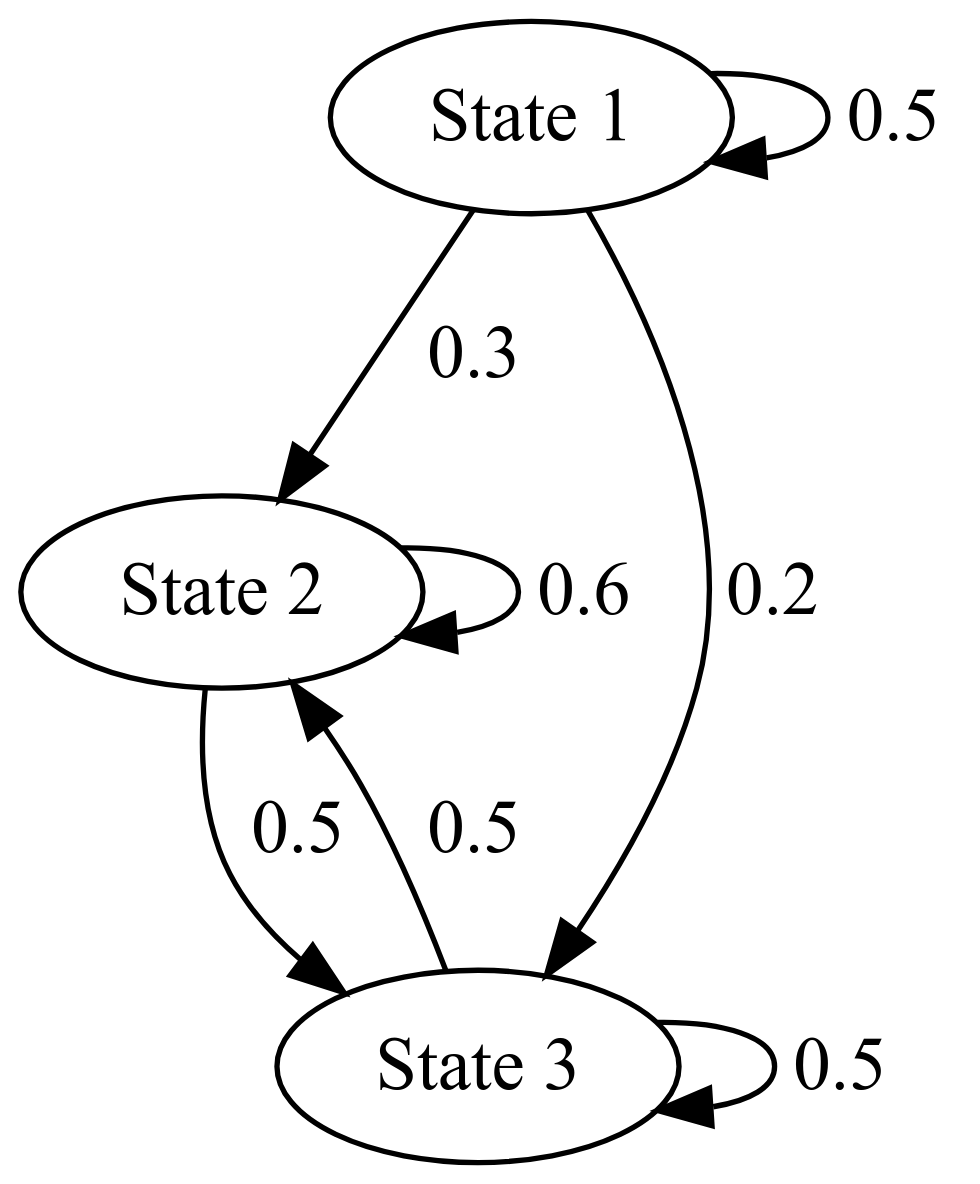
\includegraphics[width=5.5in,height=3.5in]{montecarlo_files/figure-latex/dot-figure-1.png}

}

\caption{\label{fig-P1}Graphical representation of the transition matrix
\(\mathbf{P}_1\).}

\end{figure}%

If a chain is irreducible and aperiodic, it has a unique stationary
distribution and the limiting distribution of the Markov chain will
converge there. For example, consider a transition \(\mathbf{P}_3\) on
\(1, \ldots, 5\) defined as \[
\mathbf{P}_3 = \begin{pmatrix}
\frac{2}{3} & \frac{1}{3} &  0 & 0 & 0 \\
\frac{1}{6} & \frac{2}{3} & \frac{1}{6} & 0 & 0 \\
0 & \frac{1}{6} & \frac{2}{3} & \frac{1}{6} & 0 \\
0 & 0 & \frac{1}{6} & \frac{2}{3} & \frac{1}{6} \\
0 & 0 & 0 &  \frac{1}{3}  & \frac{2}{3} \\
\end{pmatrix}
\] The stationary distribution is the value of the row vector
\(\boldsymbol{p},\) such that
\(\boldsymbol{p} = \boldsymbol{p}\mathbf{P}\) for transition matrix
\(\mathbf{P}\): we get \(\boldsymbol{p}_1=(0, 5/11, 6/11)\) for
\(\mathbf{P}_1,\) \((1/3, 1/3, 1/3)\) for \(\mathbf{P}_2\) and
\((1,2,2,2,1)/8\) for \(\mathbf{P}_3.\)

While the existence of a stationary distribution require aperiodicity,
the latter is not really important from a computational perspective as
ergodicity holds without it.

Figure~\ref{fig-discrete-markov-chain} shows the path of the random walk
driven by \(\mathbf{P}_3\) and the empirical proportion of the time
spent in each state, as time progress. Since the Markov chain has a
unique stationary distribution, we expect the sample proportions to
converge to the stationary distribution proportions.

\begin{figure}[ht!]

\centering{

\pandocbounded{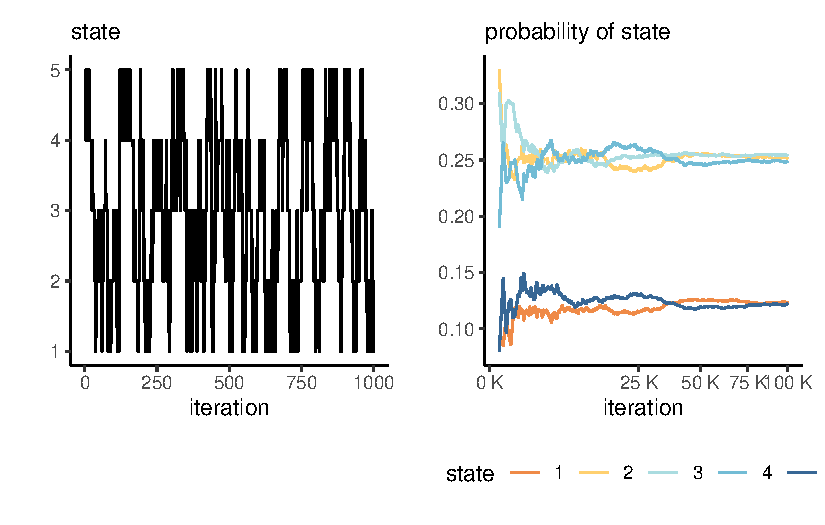
\includegraphics[keepaspectratio]{montecarlo_files/figure-pdf/fig-discrete-markov-chain-1.pdf}}

}

\caption{\label{fig-discrete-markov-chain}Discrete Markov chain on
integers from 1 to 5, with transition matrix \(\mathbf{P}_3,\) with
traceplot of 1000 first iterations (left) and running mean plots of
sample proportion of each state visited per 100 iterations (right).}

\end{figure}%

Since we will be dealing with continuous random variables in later
chapters, we use transition kernels rather than transition matrices, but
the intuition will carry forward.

\begin{definition}[Transition
kernel]\protect\hypertarget{def-transition-kernel}{}\label{def-transition-kernel}

A transition kernel
\(K(\boldsymbol{\theta}^{\text{cur}}, \boldsymbol{\theta}^{\text{prop}})\)
proposes a move from the current value
\(\boldsymbol{\theta}^{\text{cur}}\) to a proposal
\(\boldsymbol{\theta}^{\text{prop}}\).

\end{definition}

\end{proposition}

\begin{example}[Effective sample size of first-order autoregressive
process]\protect\hypertarget{exm-ar1-clt-variance}{}\label{exm-ar1-clt-variance}

The lag-\(k\) correlation of the stationary autoregressive process of
order 1 is \(\rho_k=\phi^k,\) so summing the series gives an effective
sample size for \(B\) draws of \(B(1-\phi)/(1+\phi).\) The price to pay
for having correlated samples is inefficiency: the higher the
autocorrelation, the larger the variability of our mean estimators.

\begin{figure}[ht!]

\centering{

\pandocbounded{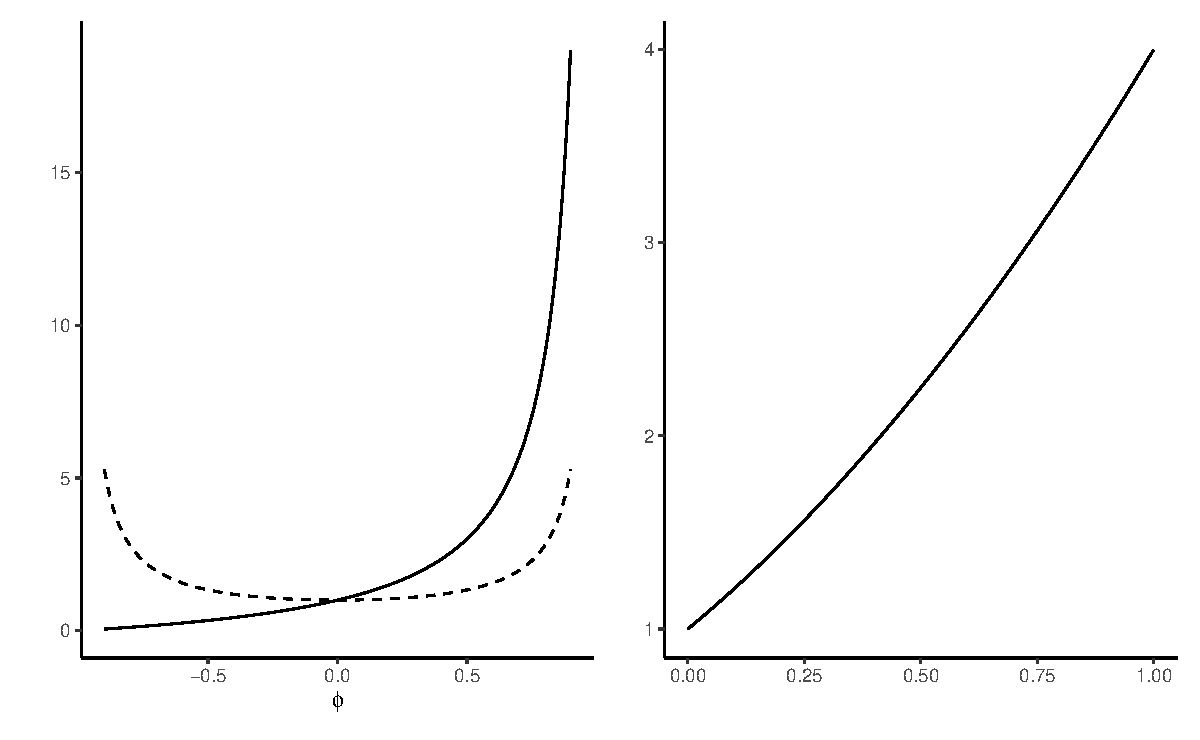
\includegraphics[keepaspectratio]{montecarlo_files/figure-pdf/fig-ar1-variance-1.pdf}}

}

\caption{\label{fig-ar1-variance}Scaled asymptotic variance of the
sample mean for a stationary autoregressive first-order process with
unit variance (full line) and a corresponding sample of independent
observations with the same marginal variance (dashed line). The right
panel gives the ratio of variances for a restricted range of positive
correlation coefficients.}

\end{figure}%

We can see from Figure~\ref{fig-ar1-variance} that, when the
autocorrelation is positive (as will be the cause in all applications of
interest), we will suffer from variance inflation. To get the same
variance estimates for the mean with an \(\mathsf{AR}(1)\) process with
\(\phi = 0.75\) than with an iid sample, we would need \(7\) times as
many observations: this is the prize to pay for autocorrelation.

\end{example}

\begin{proposition}[Uncertainty estimation with Markov
chains]\protect\hypertarget{prp-uncertainty}{}\label{prp-uncertainty}

With a simple random sample containing independent and identically
distributed observations, the standard error of the sample mean is
\(\sigma/\sqrt{n}\) and we can use the empirical standard deviation
\(\widehat{\sigma}\) to estimate the first term. For Markov chains, the
correlation prevents us from using this approach. The output of
the\texttt{coda} package are based on fitting a high order
autoregressive process to the Markov chain and using the formula of the
unconditional variance of the \(\mathsf{AR}(p)\) to obtain the central
limit theorem variance. An alternative method recommended by Geyer
(\citeproc{ref-Geyer:2011}{2011}) and implemented in his \textbf{R}
package \texttt{mcmc}, is to segment the time series into batch, compute
the means of each non-overlapping segment and use this standard
deviation with suitable rescaling to get the central limit variance for
the posterior mean. Figure~\ref{fig-mcmc-batchmean} illustrate the
method of batch means.

\begin{enumerate}
\def\labelenumi{\arabic{enumi}.}
\tightlist
\item
  Break the chain of length \(B\) (after burn in) in \(K\) blocks of
  size \(\approx K/B.\)
\item
  Compute the sample mean of each segment. These values form a Markov
  chain and should be approximately uncorrelated.
\item
  Compute the standard deviation of the segments mean. Rescale by
  \(K^{-1/2}\) to get standard error of the global mean.
\end{enumerate}

\end{proposition}

Why does the approach work? If the chain samples from the stationary
distribution, all samples have the same mean. If we partition the sample
into long enough, the sample mean of each blocks should be roughly
independent (otherwise we could remove an overlapping portion). We can
then compute the empirical standard deviation of the estimators. We can
then compute the overall mean and use a scaling argument to relate the
variability of the global estimator with the variability of the means of
the smaller blocks.

\begin{figure}[ht!]

\centering{

\pandocbounded{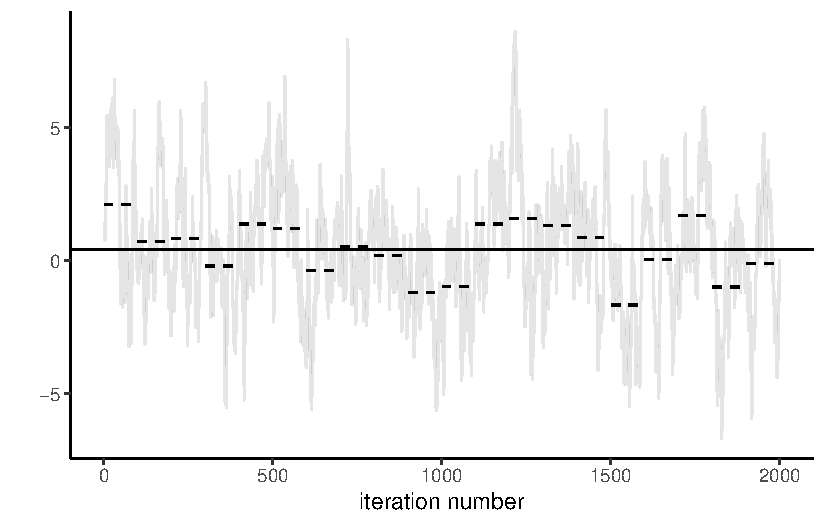
\includegraphics[keepaspectratio]{montecarlo_files/figure-pdf/fig-mcmc-batchmean-1.pdf}}

}

\caption{\label{fig-mcmc-batchmean}Calculation of the standard error of
the posterior mean using the batch method.}

\end{figure}%

\bookmarksetup{startatroot}

\chapter{Metropolis--Hastings
algorithm}\label{metropolishastings-algorithm}

The Markov chain Monte Carlo revolution in the 1990s made Bayesian
inference mainstream by allowing inference for models when only
approximations were permitted, and coincided with a time at which
computers became more widely available. The idea is to draw correlated
samples from a posterior via Markov chains, constructed to have the
posterior as invariant stationary distribution.

\begin{tcolorbox}[enhanced jigsaw, colframe=quarto-callout-important-color-frame, colback=white, leftrule=.75mm, opacitybacktitle=0.6, toprule=.15mm, colbacktitle=quarto-callout-important-color!10!white, title=\textcolor{quarto-callout-important-color}{\faExclamation}\hspace{0.5em}{\textbf{Learning objectives}:}, left=2mm, breakable, titlerule=0mm, bottomrule=.15mm, opacityback=0, bottomtitle=1mm, rightrule=.15mm, arc=.35mm, toptitle=1mm, coltitle=black]

At the end of the chapter, students should be able to

\begin{itemize}
\tightlist
\item
  implement a Metropolis--Hastings algorithm to draw samples from the
  posterior
\item
  tune proposals to obtain good mixing properties.
\end{itemize}

\end{tcolorbox}

Named after Metropolis et al. (\citeproc{ref-Metropolis:1953}{1953}),
Hastings (\citeproc{ref-Hastings:1970}{1970}), its relevance took a long
time to gain traction in the statistical community. The idea of the
Metropolis--Hastings algorithm is to construct a Markov chain targeting
a distribution \(p(\cdot).\)

\begin{proposition}[Metropolis--Hastings
algorithm]\protect\hypertarget{prp-metropolis}{}\label{prp-metropolis}

We consider from a density function \(p(\boldsymbol{\theta}),\) known up
to a normalizing factor not depending on \(\boldsymbol{\theta}.\) We use
a (conditional) proposal density
\(q(\boldsymbol{\theta} \mid \boldsymbol{\theta}^*)\) which has non-zero
probability over the support of \(p(\cdot),\) as transition kernel to
generate proposals.

The Metropolis--Hastings build a Markov chain starting from an initial
value \(\boldsymbol{\theta}_0:\)

\begin{enumerate}
\def\labelenumi{\arabic{enumi}.}
\tightlist
\item
  draw a proposal value
  \(\boldsymbol{\theta}_t^{\star} \sim q(\boldsymbol{\theta} \mid \boldsymbol{\theta}_{t-1}).\)
\item
  Compute the acceptance ratio
  \begin{equation}\phantomsection\label{eq-metropolis-ratio}{
  R = \frac{p(\boldsymbol{\theta}_t^{\star})}{p(\boldsymbol{\theta}_{t-1})}\frac{q(\boldsymbol{\theta}_{t-1} \mid \boldsymbol{\theta}_t^{\star} )}{q(\boldsymbol{\theta}_t^{\star} \mid \boldsymbol{\theta}_{t-1})}
  }\end{equation}
\item
  With probability \(\min\{R, 1\},\) accept the proposal and set
  \(\boldsymbol{\theta}_t \gets \boldsymbol{\theta}_t^{\star},\)
  otherwise set the value to the previous state,
  \(\boldsymbol{\theta}_t \gets \boldsymbol{\theta}_{t-1}.\)
\end{enumerate}

\end{proposition}

The following theoretical details provided for completeness only.

\begin{definition}[Detailed
balance]\protect\hypertarget{def-detailed-balance}{}\label{def-detailed-balance}

If our target is \(p(\cdot),\) then the Markov chain satisfies the
\textbf{detailed balance} condition with respect to \(p(\cdot)\) if
\begin{align*}
K(\boldsymbol{\theta}^{\text{cur}}, \boldsymbol{\theta}^{\text{prop}})p(\boldsymbol{\theta}^{\text{cur}}) = K(\boldsymbol{\theta}^{\text{prop}}, \boldsymbol{\theta}^{\text{cur}})p(\boldsymbol{\theta}^{\text{prop}}).
\end{align*} If a Markov chain satisfies the detailed balance with
respect to \(p(\cdot),\) then the latter is necessarily the invariant
density of the Markov chain and the latter is reversible.

\end{definition}

\begin{proposition}[Metropolis--Hastings satisfies detailed
balance]\protect\hypertarget{prp-detailed-balance-mh}{}\label{prp-detailed-balance-mh}

The Metropolis--Hastings algorithm has transition kernel for a move from
\(\boldsymbol{x}\) to a proposal \(\boldsymbol{y}\) \begin{align*}
K(\boldsymbol{x}, \boldsymbol{y}) = \alpha(\boldsymbol{x}, \boldsymbol{y}) q(\boldsymbol{y} \mid \boldsymbol{x}) + \{1- r(\boldsymbol{x})\}\mathsf{I}(\boldsymbol{y}=\boldsymbol{x})
\end{align*} where
\(r(\boldsymbol{x})=\int \alpha(\boldsymbol{x}, \boldsymbol{y}) q(\boldsymbol{y} \mid \boldsymbol{x})\mathrm{d} \boldsymbol{y}\)
is the average probability of acceptance of a move from
\(\boldsymbol{x},\) \(\mathsf{I}(\cdot = \boldsymbol{x})\) is a point
mass at \(\boldsymbol{x},\) and \(\alpha(\cdot)\) is defined on the next
slide.

One can show that the Metropolis--Hastings algorithm satisfies detailed
balanced; see, e.g., Theorem 7.2 of Robert and Casella
(\citeproc{ref-Casella.Robert:2004}{2004}).

\end{proposition}

If \(\boldsymbol{\theta}_{t}\) is drawn from the posterior, then the
left hand side is the joint density of
\((\boldsymbol{\theta}_{t}, \boldsymbol{\theta}_{t+1})\) and the
marginal distribution obtained by integrating over
\(\boldsymbol{\theta}_{t},\) \begin{align*}
\int f(\boldsymbol{\theta}_{t+1} \mid \boldsymbol{\theta}_{t})p(\boldsymbol{\theta}_{t} \mid \boldsymbol{y})\mathrm{d} \boldsymbol{\theta}_{t}
& = \int f(\boldsymbol{\theta}_{t} \mid \boldsymbol{\theta}_{t+1})p(\boldsymbol{\theta}_{t+1} \mid \boldsymbol{y})\mathrm{d} \boldsymbol{\theta}_{t} 
\\&\quad= p(\boldsymbol{\theta}_{t+1} \mid \boldsymbol{y})
\end{align*} and any draw from the posterior will generate a new
realization from the posterior. It also ensures that, provided the
starting value has non-zero probability under the posterior, the chain
will converge to the stationarity distribution (albeit perhaps slowly).

\begin{remark}[Interpretation of the algorithm]
If \(R>1,\) the proposal has higher density and we always accept the
move. If the ratio is less than one, the proposal is in a lower
probability region, we accept the move with probability \(R\) and set
\(\boldsymbol{\theta}_{t}=\boldsymbol{\theta}^{\star}_t\); if we reject,
the Markov chain \emph{stays at the current value}, which induces
autocorrelation. Since the acceptance probability depends only on the
density through ratios, we can work with unnormalized density functions
and this is what allows us, if our proposal density is the (marginal)
posterior of the parameter, to obtain approximate posterior samples
without having to compute the marginal likelihood.
\end{remark}

\begin{remark}[Blank run]
To check that the algorithm is well-defined, we can remove the log
likelihood component and run the algorithm: if it is correct, the
resulting draws should be drawn from the prior provided the latter is
proper (\citeproc{ref-Green:2001}{Green 2001, 55}).
\end{remark}

\begin{remark}[Symmetric proposals]
Suppose we generate a candidate sample \(\boldsymbol{\theta}_t^{\star}\)
from a symmetric distribution \(q(\cdot \mid \cdot)\) centered at
\(\boldsymbol{\theta}_{t-1},\) such as the random walk
\(\boldsymbol{\theta}_t^{\star} =\boldsymbol{\theta}_{t-1}+ Z\) where
\(Z\) has a symmetric distribution. Then, the proposal density ratio
cancels so need not be computed in the Metropolis ratio of
Equation~\ref{eq-metropolis-ratio}.
\end{remark}

\begin{remark}[Calculations]
In practice, we compute the log of the acceptance ratio, \(\ln R,\) to
avoid numerical overflow. If our target is log posterior density, we
have \[
\ln \left\{\frac{p(\boldsymbol{\theta}_t^{\star})}{p(\boldsymbol{\theta}_{t-1})}\right\} = \ell(\boldsymbol{\theta}_t^{\star}) + \ln p(\boldsymbol{\theta}_t^{\star}) - \ell(\boldsymbol{\theta}_{t-1}) - \ln p(\boldsymbol{\theta}_{t-1}) 
\] and we proceed likewise for the log of the ratio of transition
kernels. We then compare the value of \(\ln R\) (if less than zero) to
\(\log(U),\) where \(U \sim \mathsf{U}(0,1).\) We accept the move if
\(\ln(R) >\log(U)\) and keep the previous value otherwise.
\end{remark}

\begin{example}[]\protect\hypertarget{exm-upworthy-question}{}\label{exm-upworthy-question}

Consider again the Upworthy data from
Example~\ref{exm-poisson-upworthy-question}. We model the Poisson rates
\(\lambda_i\) \((i=1,2),\) this time with the usual Poisson regression
parametrization in terms of log rate for the baseline \text{yes},
\(\log(\lambda_2) = \beta,\) and log odds rates
\(\kappa = \log(\lambda_1) - \log(\lambda_2).\) Our model is
\begin{align*}
Y_{i} &\sim \mathsf{Po}(n_i\lambda_i), \qquad (i=1,2)\\
\lambda_1 &= \exp(\beta + \kappa) \\
\lambda_2 &= \exp(\beta) \\
\beta & \sim \mathsf{Gauss}(\log 0.01, 1.5) \\
\kappa &\sim \mathsf{Gauss}(0, 1)
\end{align*} There are two parameters in the model, which can be updated
in turn or jointly.

\begin{Shaded}
\begin{Highlighting}[]
\FunctionTok{data}\NormalTok{(upworthy\_question, }\AttributeTok{package =} \StringTok{"hecbayes"}\NormalTok{)}
\CommentTok{\# Compute sufficient statistics}
\NormalTok{data }\OtherTok{\textless{}{-}}\NormalTok{ upworthy\_question }\SpecialCharTok{|\textgreater{}}
\NormalTok{  dplyr}\SpecialCharTok{::}\FunctionTok{group\_by}\NormalTok{(question) }\SpecialCharTok{|\textgreater{}}
\NormalTok{  dplyr}\SpecialCharTok{::}\FunctionTok{summarize}\NormalTok{(}\AttributeTok{ntot =} \FunctionTok{sum}\NormalTok{(impressions),}
                   \AttributeTok{y =} \FunctionTok{sum}\NormalTok{(clicks))}
\CommentTok{\# Code log posterior as sum of log likelihood and log prior}
\NormalTok{loglik }\OtherTok{\textless{}{-}} \ControlFlowTok{function}\NormalTok{(par, }\AttributeTok{counts =}\NormalTok{ data}\SpecialCharTok{$}\NormalTok{y, }\AttributeTok{offset =}\NormalTok{ data}\SpecialCharTok{$}\NormalTok{ntot, ...)\{}
\NormalTok{  lambda }\OtherTok{\textless{}{-}} \FunctionTok{exp}\NormalTok{(}\FunctionTok{c}\NormalTok{(par[}\DecValTok{1}\NormalTok{] }\SpecialCharTok{+} \FunctionTok{log}\NormalTok{(offset[}\DecValTok{1}\NormalTok{]), par[}\DecValTok{1}\NormalTok{] }\SpecialCharTok{+}\NormalTok{ par[}\DecValTok{2}\NormalTok{] }\SpecialCharTok{+} \FunctionTok{log}\NormalTok{(offset[}\DecValTok{2}\NormalTok{])))}
 \FunctionTok{sum}\NormalTok{(}\FunctionTok{dpois}\NormalTok{(}\AttributeTok{x =}\NormalTok{ counts, }\AttributeTok{lambda =}\NormalTok{ lambda, }\AttributeTok{log =} \ConstantTok{TRUE}\NormalTok{))}
\NormalTok{\}}
\NormalTok{logprior }\OtherTok{\textless{}{-}} \ControlFlowTok{function}\NormalTok{(par, ...)\{}
  \FunctionTok{dnorm}\NormalTok{(}\AttributeTok{x =}\NormalTok{ par[}\DecValTok{1}\NormalTok{], }\AttributeTok{mean =} \FunctionTok{log}\NormalTok{(}\FloatTok{0.01}\NormalTok{), }\AttributeTok{sd =} \FloatTok{1.5}\NormalTok{, }\AttributeTok{log =} \ConstantTok{TRUE}\NormalTok{) }\SpecialCharTok{+}
    \FunctionTok{dnorm}\NormalTok{(}\AttributeTok{x =}\NormalTok{ par[}\DecValTok{2}\NormalTok{], }\AttributeTok{log =} \ConstantTok{TRUE}\NormalTok{)}
\NormalTok{\}}
\NormalTok{logpost }\OtherTok{\textless{}{-}} \ControlFlowTok{function}\NormalTok{(par, ...)\{}
  \FunctionTok{loglik}\NormalTok{(par, ...) }\SpecialCharTok{+} \FunctionTok{logprior}\NormalTok{(par, ...)}
\NormalTok{\}}
\CommentTok{\# Compute maximum a posteriori (MAP)}
\NormalTok{map }\OtherTok{\textless{}{-}} \FunctionTok{optim}\NormalTok{(}
  \AttributeTok{par =} \FunctionTok{c}\NormalTok{(}\SpecialCharTok{{-}}\DecValTok{4}\NormalTok{, }\FloatTok{0.07}\NormalTok{),}
  \AttributeTok{fn =}\NormalTok{ logpost,}
  \AttributeTok{control =} \FunctionTok{list}\NormalTok{(}\AttributeTok{fnscale =} \SpecialCharTok{{-}}\DecValTok{1}\NormalTok{),}
  \AttributeTok{offset =}\NormalTok{ data}\SpecialCharTok{$}\NormalTok{ntot,}
  \AttributeTok{counts =}\NormalTok{ data}\SpecialCharTok{$}\NormalTok{y,}
  \AttributeTok{hessian =} \ConstantTok{TRUE}\NormalTok{)}
\CommentTok{\# Use MAP as starting value}
\NormalTok{cur }\OtherTok{\textless{}{-}}\NormalTok{ map}\SpecialCharTok{$}\NormalTok{par}
\CommentTok{\# Compute logpost\_cur {-} we can keep track of this to reduce calculations}
\NormalTok{logpost\_cur }\OtherTok{\textless{}{-}} \FunctionTok{logpost}\NormalTok{(cur)}
\CommentTok{\# Proposal covariance}
\NormalTok{cov\_map }\OtherTok{\textless{}{-}} \SpecialCharTok{{-}}\DecValTok{2}\SpecialCharTok{*}\FunctionTok{solve}\NormalTok{(map}\SpecialCharTok{$}\NormalTok{hessian)}
\NormalTok{chol }\OtherTok{\textless{}{-}} \FunctionTok{chol}\NormalTok{(cov\_map)}

\FunctionTok{set.seed}\NormalTok{(}\DecValTok{80601}\NormalTok{)}
\NormalTok{niter }\OtherTok{\textless{}{-}} \FloatTok{1e4}\NormalTok{L}
\NormalTok{chain }\OtherTok{\textless{}{-}} \FunctionTok{matrix}\NormalTok{(}\DecValTok{0}\NormalTok{, }\AttributeTok{nrow =}\NormalTok{ niter, }\AttributeTok{ncol =} \DecValTok{2}\NormalTok{L)}
\FunctionTok{colnames}\NormalTok{(chain) }\OtherTok{\textless{}{-}} \FunctionTok{c}\NormalTok{(}\StringTok{"beta"}\NormalTok{,}\StringTok{"kappa"}\NormalTok{)}
\NormalTok{naccept }\OtherTok{\textless{}{-}} \DecValTok{0}\NormalTok{L}
\ControlFlowTok{for}\NormalTok{(i }\ControlFlowTok{in} \FunctionTok{seq\_len}\NormalTok{(niter))\{}
  \CommentTok{\# Multivariate normal proposal {-} symmetric random walk}
\NormalTok{  prop }\OtherTok{\textless{}{-}}\NormalTok{ chol }\SpecialCharTok{\%*\%} \FunctionTok{rnorm}\NormalTok{(}\AttributeTok{n =} \DecValTok{2}\NormalTok{) }\SpecialCharTok{+}\NormalTok{ cur}
\NormalTok{  logpost\_prop }\OtherTok{\textless{}{-}} \FunctionTok{logpost}\NormalTok{(prop)}
  \CommentTok{\# Compute acceptance ratio (no q because the ratio is 1)}
\NormalTok{  logR }\OtherTok{\textless{}{-}}\NormalTok{ logpost\_prop }\SpecialCharTok{{-}}\NormalTok{ logpost\_cur}
  \ControlFlowTok{if}\NormalTok{(logR }\SpecialCharTok{\textgreater{}} \SpecialCharTok{{-}}\FunctionTok{rexp}\NormalTok{(}\DecValTok{1}\NormalTok{))\{}
\NormalTok{    cur }\OtherTok{\textless{}{-}}\NormalTok{ prop}
\NormalTok{    logpost\_cur }\OtherTok{\textless{}{-}}\NormalTok{ logpost\_prop}
\NormalTok{    naccept }\OtherTok{\textless{}{-}}\NormalTok{ naccept }\SpecialCharTok{+} \DecValTok{1}\NormalTok{L}
\NormalTok{  \}}
\NormalTok{  chain[i,] }\OtherTok{\textless{}{-}}\NormalTok{ cur}
\NormalTok{\}}
\CommentTok{\# Posterior summaries}
\FunctionTok{summary}\NormalTok{(coda}\SpecialCharTok{::}\FunctionTok{as.mcmc}\NormalTok{(chain))}
\end{Highlighting}
\end{Shaded}

\begin{verbatim}

Iterations = 1:10000
Thinning interval = 1 
Number of chains = 1 
Sample size per chain = 10000 

1. Empirical mean and standard deviation for each variable,
   plus standard error of the mean:

          Mean       SD  Naive SE Time-series SE
beta  -4.51268 0.001697 1.697e-05      6.176e-05
kappa  0.07075 0.002033 2.033e-05      9.741e-05

2. Quantiles for each variable:

          2.5%      25%      50%      75%    97.5%
beta  -4.51591 -4.51385 -4.51273 -4.51154 -4.50929
kappa  0.06673  0.06933  0.07077  0.07212  0.07463
\end{verbatim}

\begin{Shaded}
\begin{Highlighting}[]
\CommentTok{\# Computing standard errors using batch means}
\FunctionTok{sqrt}\NormalTok{(}\FunctionTok{diag}\NormalTok{(mcmc}\SpecialCharTok{::}\FunctionTok{olbm}\NormalTok{(chain, }\AttributeTok{batch.length =}\NormalTok{ niter}\SpecialCharTok{/}\DecValTok{40}\NormalTok{)))}
\end{Highlighting}
\end{Shaded}

\begin{verbatim}
[1] 5.717097e-05 8.220816e-05
\end{verbatim}

The acceptance rate of the algorithm is 35.1\% and the posterior means
are \(\beta =-4.51\) and \(\kappa =0.07.\)

\begin{figure}[ht!]

\centering{

\pandocbounded{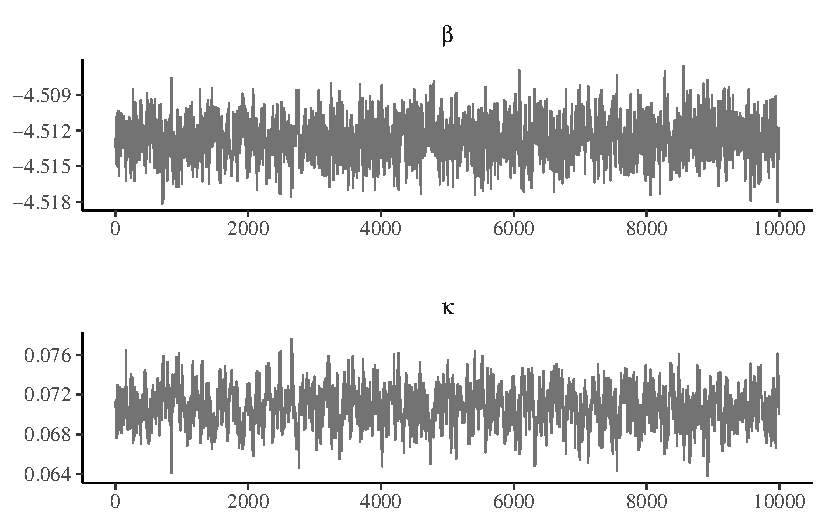
\includegraphics[keepaspectratio]{mcmc_files/figure-pdf/fig-traceplot-1.pdf}}

}

\caption{\label{fig-traceplot}Traceplots of Markov chain of log rate and
log odds rate for the Metropolis--Hastings sampler applied to the
Upworthy question data.}

\end{figure}%

Figure~\ref{fig-scatterplot-upworthy-question} shows the posterior
samples, which are very nearly bivariate Gaussian. The parametrization
in terms of log odds ratio induces strong negative dependence, so if we
were to sample \(\kappa,\) then \(\beta,\) we would have much larger
inefficiency and slower exploration. Instead, the code used a bivariate
Gaussian random walk proposal whose covariance matrix was taken as a
multiple of the inverse of the negative hessian (equivalently, to the
observed information matrix of the log posterior), evaluated at of the
maximum a posteriori. This Gaussian approximation is called
\textbf{Laplace approximation}: it is advisable to reparametrize the
model so that the distribution is nearly symmetric, so that the
approximation is good. In this example, because of the large sample, the
Gaussian approximation implied by Bernstein--von Mises' theorem is
excellent.

\begin{figure}[ht!]

\centering{

\pandocbounded{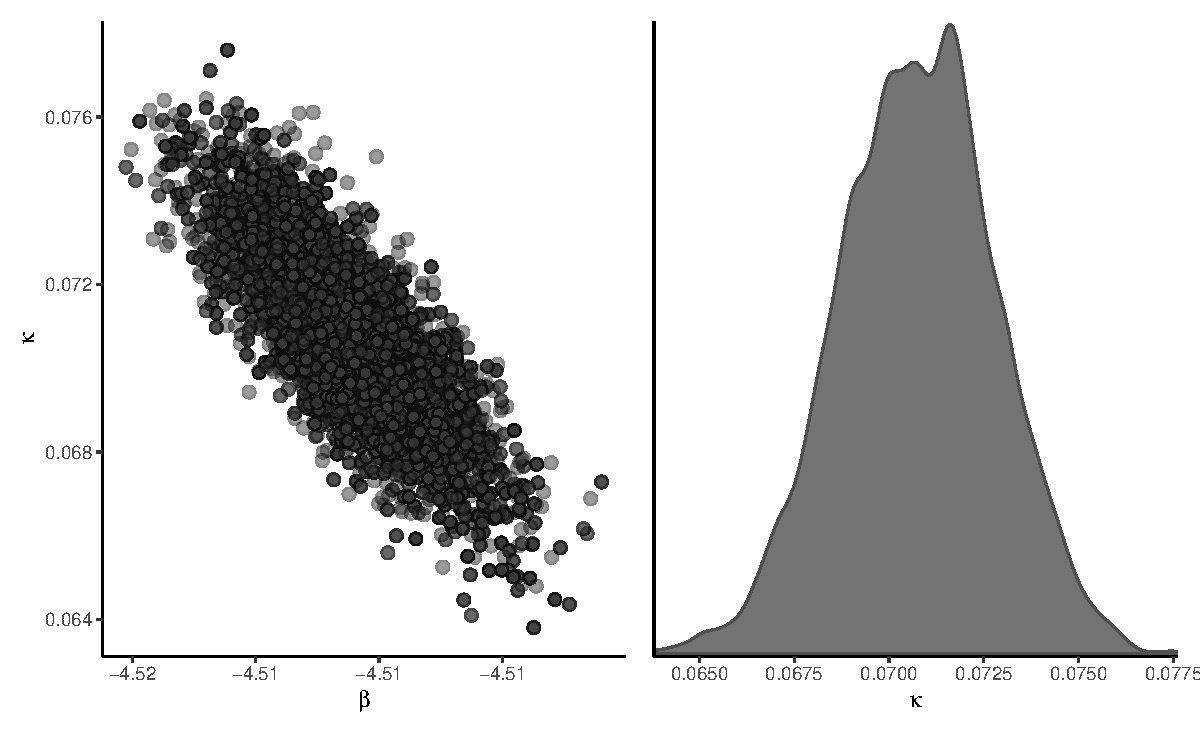
\includegraphics[keepaspectratio]{mcmc_files/figure-pdf/fig-scatterplot-upworthy-question-1.pdf}}

}

\caption{\label{fig-scatterplot-upworthy-question}Scatterplot of
posterior draws (left) and marginal density plot of log odds rate
(right).}

\end{figure}%

\end{example}

\begin{refremark}[Reparametrization]
A better parametrization would simply sample two parameters with
\(\lambda_2 = \exp(\alpha),\) where \(\alpha\) is the log mean of the
second group, with the same prior as for \(\beta.\) Since the likelihood
factorizes and the parameters are independent apriori, this would lead
to zero correlation and lead to more efficient mixing of the Markov
chain, should we wish to sample parameters in turn one at the time. A
Markov chain for \(\kappa\) can then be obtained by substracting the
values of \(\alpha-\beta\) from the new draws.

\label{rem-reparametrization}

\end{refremark}

The quality of the mixing of the chain (autocorrelation), depends on the
proposal variance, which can obtain by trial and error. Trace plots
Figure~\ref{fig-traceplot} show the values of the chain as a function of
iteration number. If our algorithm works well, we expect the proposals
to center around the posterior mode and resemble a fat hairy
caterpillar. If the variance is too small, the acceptance rate will
increase but most steps will be small. If the variance of the proposal
is too high, the acceptance rate will decrease (as many proposal moves
will have much lower posterior), so the chain will get stuck for long
periods of time. This is Goldilock's principle, as illustrated in
Figure~\ref{fig-goldilock-trace}.

\begin{figure}[ht!]

\centering{

\pandocbounded{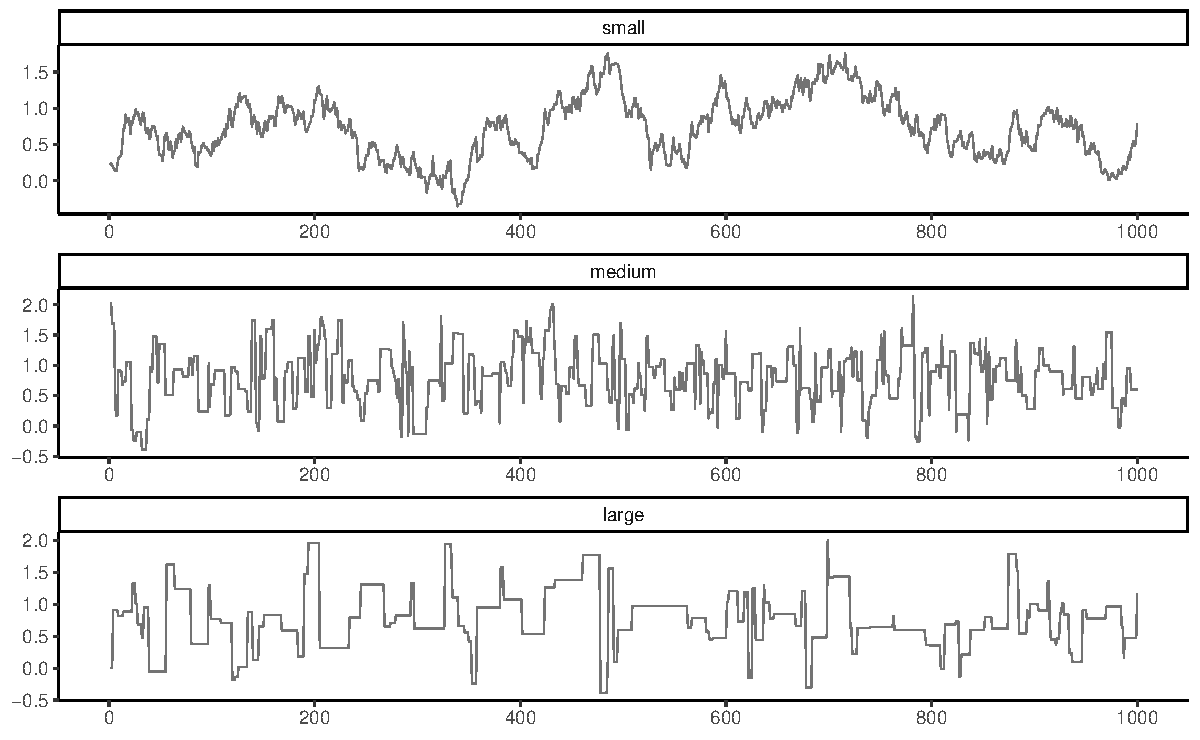
\includegraphics[keepaspectratio]{mcmc_files/figure-pdf/fig-goldilock-trace-1.pdf}}

}

\caption{\label{fig-goldilock-trace}Example of traceplot with proposal
variance that is too small (top), adequate (middle) and too large
(bottom).}

\end{figure}%

One way to calibrate is to track the acceptance rate of the proposals:
for the three chains in Figure~\ref{fig-goldilock-trace}, these are
0.932, 0.33, 0.12. In one-dimensional toy problems with Gaussian
distributions, an acceptance rate of 0.44 is optimal, and this ratio
decreases to 0.234 when \(D \geq 2\)
(\citeproc{ref-Roberts.Rosenthal:2001}{Roberts and Rosenthal 2001};
\citeproc{ref-Sherlock:2013}{Sherlock 2013}). This need not generalize
to other settings and depends on the context. Optimal rate for
alternative algorithms, such as Metropolis-adjusted Langevin algorithm,
are typically higher.

We can tune the variance of the global proposal
(\citeproc{ref-Andrieu.Thoms:2008}{Andrieu and Thoms 2008}) to improve
the mixing of the chains at approximate stationarity. This is done by
increasing (decreasing) the variance if the historical acceptance rate
is too high (respectively low) during the burn in period, and
reinitializing after any change with an acceptance target of \(0.44.\)
We stop adapting to ensure convergence to the posterior after a suitable
number of initial iterations. Adaptive MCMC methods use an initial warm
up period to find good proposals: we can consider a block of length
\(L,\) compute the acceptance rate, multiply the variance by a scaling
factor and run the chain a little longer. We only keep samples obtained
after the adaptation phase.

We can also plot the autocorrelation of the entries of the chain as a
function of lags, a display known as correlogram in the time series
literature but colloquially referred to as autocorrelation function
(acf). The higher the autocorrelation, the more variance inflation one
has and the longer the number of steps before two draws are treated as
independent. Figure~\ref{fig-goldilock-correlogram} shows the effect of
the proposal variance on the correlation for the three chains.
Practitioners designing very inefficient Markov chain Monte Carlo
algorithms often thin their series: that is, they keep only every \(k\)
iteration. This is not recommended practice unless storage is an issue
and usually points towards inefficient sampling algorithms.

\begin{figure}[ht!]

\centering{

\pandocbounded{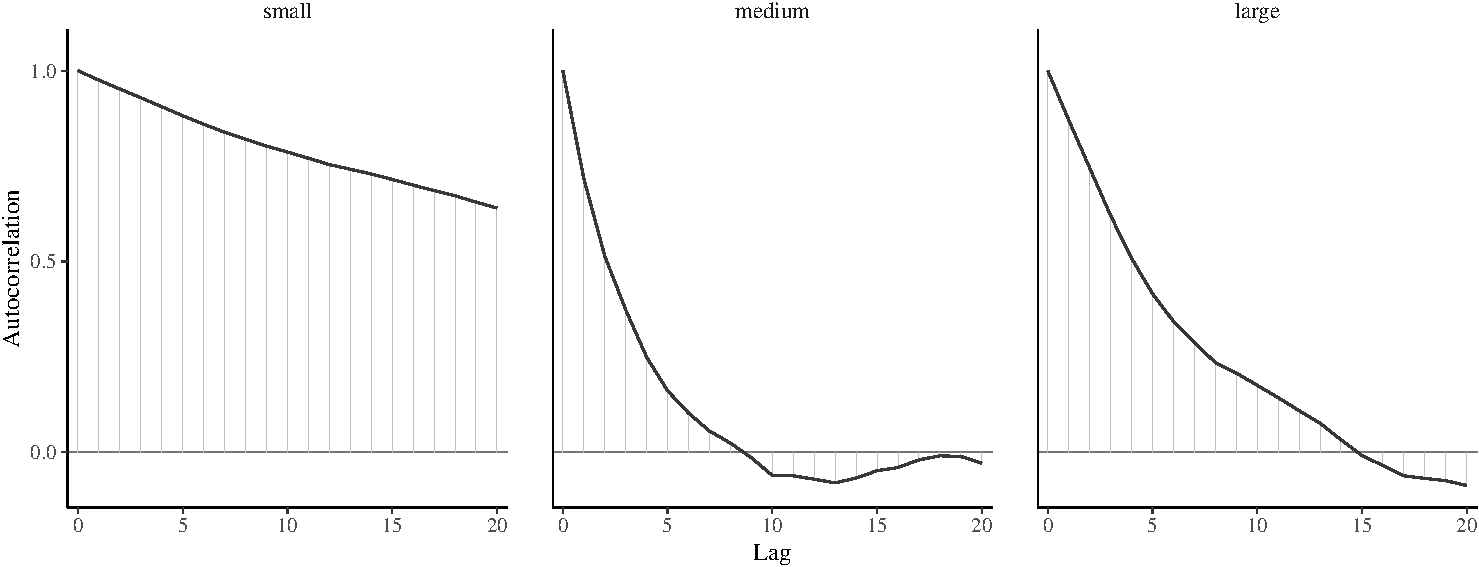
\includegraphics[keepaspectratio]{mcmc_files/figure-pdf/fig-goldilock-correlogram-1.pdf}}

}

\caption{\label{fig-goldilock-correlogram}Correlogram for the three
Markov chains.}

\end{figure}%

\begin{remark}[Independence Metropolis--Hastings]
If the proposal density \(q(\cdot)\) does not depend on the current
state \(\boldsymbol{\theta}_{t-1},\) the algorithm is termed
\emph{independence}. To maximize acceptance, we could design a candidate
distribution whose mode is at the maximum a posteriori value. To
efficiently explore the state space, we need to place enough density in
all regions, for example by taking a heavy-tailed distributions, so that
we explore the full support. Such proposals can be however inefficient
and fail when the distribution of interest is multimodal. The
independence Metropolis--Hastings algorithm then resembles
accept-reject. If the ratio
\(p(\boldsymbol{\theta})/q(\boldsymbol{\theta})\) is bounded above by
\(C \geq 1,\) then we can make comparisons with rejection sampling.
Lemma 7.9 of Robert and Casella
(\citeproc{ref-Casella.Robert:2004}{2004}) shows that the probability of
acceptance of a move for the Markov chain is at least \(1/C,\) which is
larger than the accept-reject.
\end{remark}

In models with multiple parameter, we can use Metropolis--Hastings
algorithm to update every parameter in turn, fixing the value of the
others, rather than update them in block. The reason behind this
pragmatic choice is that, as for ordinary Monte Carlo sampling, the
acceptance rate goes down sharply with the dimension of the vector.
Updating parameters one at a time can lead to higher acceptance rates,
but slower exploration as a result of the correlation between
parameters.

If we can factorize the log posterior, then some updates may not depend
on all parameters: in a hierarchical model, hyperpriors parameter only
appear through priors, etc. This can reduce computational costs.

\begin{proposition}[Parameter
transformation]\protect\hypertarget{prp-parameter-transformation}{}\label{prp-parameter-transformation}

If a parameter is bounded in the interval \((a,b),\) where
\(-\infty \leq a < b \leq \infty,\) we can consider a bijective
transformation \(\vartheta \equiv t(\theta): (a,b) \to \mathbb{R}\) with
differentiable inverse. The log density of the transformed variable,
assuming it exists, is \begin{align*}
f_\vartheta(\vartheta) = f_{\theta}\{t^{-1}(\vartheta)\} \left| \frac{\mathrm{d}}{\mathrm{d} \vartheta} t^{-1}(\vartheta)\right|
\end{align*} For example, we can use of the following transformations
for finite \(a, b\) in the software:

\begin{itemize}
\tightlist
\item
  if \(\theta \in (a, \infty)\) (lower bound only), then
  \(\vartheta = \log(\theta-a)\) and
  \(f_{\vartheta}(\vartheta)=f_{\theta}\{\exp(\vartheta) + a\}\cdot \exp(\vartheta)\)
\item
  if \(\theta \in (-\infty, b)\) (upper bound only), then
  \(\vartheta = \log(b-\theta)\) and
  \(f_{\vartheta}(\vartheta)=f_{\theta}\{b-\exp(\vartheta)\}\cdot \exp(\vartheta)\)
\item
  if \(\theta \in (a, b)\) (both lower and upper bound), then
  \(\vartheta = \mathrm{logit}\{(\theta-a)/(b-a)\}\) and \begin{align*}
  f_{\vartheta}(\vartheta)&=f_{\theta}\{a+(b-a) \mathrm{expit}(\vartheta)\} (b-a)\\&\quad \times \mathrm{expit}(\vartheta)\{1-\mathrm{expit}(\vartheta)\}
  \end{align*}
\end{itemize}

To guarantee that our proposals fall in the support of \(\theta,\) we
can thus run a symmetric random walk proposal on the \emph{transformed
scale} by drawing \(\vartheta_{t}^{\star} \sim \vartheta_{t-1}+\tau Z\)
where \(Z\sim\mathsf{Gauss}(0, 1).\) Due to the transformation, the
kernel ratio now contains the Jacobian.

\end{proposition}

\begin{proposition}[Truncated
proposals]\protect\hypertarget{prp-truncated-proposals}{}\label{prp-truncated-proposals}

As an alternative, if we are dealing with parameters that are restricted
in \([a,b],\) we can simulate using a random walk but with truncated
Gaussian steps, taking
\(\theta^{\star}_{t} \sim \mathsf{trunc. Gauss}(\vartheta_{t-1}, \tau^2, a, b).\)
The benefits of using the truncated proposal becomes more apparent when
we move to more advanced proposals whose mean and variance depends on
the gradient and or the hessian of the underlying unnormalized log
posterior, as the mean can be lower than \(a\) or larger than \(b\):
this would garantee zero acceptance with regular Gaussian random walk.
The \texttt{TruncatedNormal} package can be used to efficiently evaluate
such instances using results from Botev and L'Écuyer
(\citeproc{ref-LEcuyer.Botev:2017}{2017}) even when the truncation
bounds are far from the mode. the normalizing constant of the truncated
Gaussian in the denominator of the density is a function of the location
and scale parameters: if these depend on the current value of
\(\boldsymbol{\theta}_{t-1},\) as is the case for a random walk, we need
to keep these terms as part of the Metropolis ratio. The mean and
standard deviation of the truncated Gaussian are not equal to the
parameters \(\mu\) (which corresponds to the mode, provided
\(a < \mu < b\)) and \(\sigma.\)

\end{proposition}

\begin{proposition}[Efficient
proposals]\protect\hypertarget{prp-mala}{}\label{prp-mala}

Rather than simply build a random walk, we can exploit the geometry of
the posterior using the gradient, via Metropolis-ajusted Langevin
algorithm (MALA), or using local quadratic approximations of the target.

Let \(p(\theta)\) denote the conditional (unnormalized) log posterior
for a scalar parameter \(\theta \in (a, b).\) We considering a Taylor
series expansion of \(p(\cdot)\) around the current parameter value
\(\theta_{t-1},\) \begin{align*}
 p(\theta) \approx p(\theta_{t-1}) + p'(\theta_{t-1})(\theta - \theta_{t-1}) + \frac{1}{2} p''(\theta_{t-1})(\theta - \theta_{t-1})^2
\end{align*} plus remainder, which suggests a Gaussian approximation
with mean
\(\mu_{t-1} = \theta_{t-1} - f'(\theta_{t-1})/f''(\theta_{t-1})\) and
precision \(\tau^{-2} = -f''(\theta_{t-1}).\) We can use truncated
Gaussian distribution on \((a, b)\) with mean \(\mu\) and standard
deviation \(\tau,\) denoted \(\mathsf{trunc. Gauss}(\mu, \tau, a, b)\)
with corresponding density function \(q(\cdot; \mu, \tau, a, b).\) The
Metropolis acceptance ratio for a proposal
\(\theta^{\star}_{t} \sim \mathsf{trunc. Gauss}(\mu_{t-1}, \tau_{t-1}, a, b)\)
is \begin{align*}
 \alpha = \frac{p(\theta^{\star}_{t})}{p(\theta_{t-1})} \frac{ q(\theta_{t-1} \mid \mu_{t}^{\star}, \tau_{t}^{\star}, a, b)}{q(\theta^{\star}_{t} \mid \mu_{t-1}, \tau_{t-1}, a, b)}
\end{align*} and we set \(\theta^{(t+1)} = \theta^{\star}_{t}\) with
probability \(\min\{1, r\}\) and \(\theta^{(t+1)} = \theta_{t-1}\)
otherwise. To evaluate the ratio of truncated Gaussian densities
\(q(\cdot; \mu, \tau, a, b),\) we need to compute the Taylor
approximation from the current parameter value, but also the reverse
move from the proposal \(\theta^{\star}_{t}.\) Another option is to
modify the move dictated by the rescaled gradient by taking instead
\[\mu_{t-1} = \theta_{t-1} - \eta f'(\theta_{t-1})/f''(\theta_{t-1}).\]
The proposal includes an additional learning rate parameter,
\(\eta \leq 1,\) whose role is to prevent oscillations of the quadratic
approximation, as in a Newton--Raphson algorithm. Relative to a random
walk Metropolis--Hastings, the proposal automatically adjusts to the
local geometry of the target, which guarantees a higher acceptance rate
and lower autocorrelation for the Markov chain despite the higher
evaluation costs. The proposal requires that both \(f''(\theta_{t-1})\)
and \(f''(\theta^{\star}_{t})\) be negative since the variance is
\(-1/f''(\theta)\): this shouldn't be problematic in the vicinity of the
mode. Otherwise, one could use a global scaling derived from the hessian
at the mode (\citeproc{ref-Rue.Held:2005}{H. Rue and Held 2005}).

The simpler Metropolis-adjusted Langevin algorithm is equivalent to
using a Gaussian random walk where the proposal has mean
\(\boldsymbol{\theta}_{t-1} + \mathbf{A}\eta \nabla \log p(\boldsymbol{\theta}_{t-1}; \boldsymbol{y})\)
and variance \(\tau^2\mathbf{A},\) for some mass matrix \(\mathbf{A}\)
and learning rate \(\eta < 1.\) Taking \(\mathbf{A}\) as the identity
matrix, which assumes the parameters are isotropic (same variance,
uncorrelated) is the default choice although seldom far from optimal.

For MALA to work well, we need both to start near stationarity, to
ensure that the gradient is relatively small and to prevent
oscillations. One can dampen the size of the step initially if needed to
avoid overshooting. The proposal variance, the other tuning parameter,
is critical to the success of the algorithm. The usual target for the
variance is one that gives an acceptance rate of roughly 0.574. These
more efficient methods require additional calculations of the gradient
and Hessian, either numerically or analytically. Depending on the
situation and the computational costs of such calculations, the
additional overhead may not be worth it.

\end{proposition}

\begin{example}[]\protect\hypertarget{exm-normal-question-upworthy}{}\label{exm-normal-question-upworthy}

We revisit the Upworthy data, this time modelling each individual
headline as a separate observation. We view \(n=\)\texttt{nimpression}
as the sample size of a binomial distribution and \texttt{nclick} as the
number of successes. Since the number of trials is large, the sample
average \texttt{nclick}/\texttt{nimpression}, denoted \(y\) in the
sequel, is approximately Gaussian. We assume that each story has a
similar population rate and capture the heterogeneity inherent to each
news story by treating each mean as a sample. The variance of the sample
average or click rate is proportional to \(n^{-1},\) where \(n\) is the
number of impressions. To allow for underdispersion or overdispersion,
we thus consider a Gaussian likelihood
\(Y_i \sim \mathsf{Gauss}(\mu, \sigma^2/n_i).\) We perform Bayesian
inference for \(\mu, \sigma\) after assigning a truncated Gaussian prior
for \(\mu \sim \mathsf{trunc. Gauss}(0.01, 0.1^2)\) over \([0,1]\) and
an penalized complexity prior for \(\sigma \sim \mathsf{Exp}(0.7).\)

\begin{Shaded}
\begin{Highlighting}[]
\FunctionTok{data}\NormalTok{(upworthy\_question, }\AttributeTok{package =} \StringTok{"hecbayes"}\NormalTok{)}
\CommentTok{\# Select data for a single question}
\NormalTok{qdata }\OtherTok{\textless{}{-}}\NormalTok{ upworthy\_question }\SpecialCharTok{|\textgreater{}}
\NormalTok{  dplyr}\SpecialCharTok{::}\FunctionTok{filter}\NormalTok{(question }\SpecialCharTok{==} \StringTok{"yes"}\NormalTok{) }\SpecialCharTok{|\textgreater{}}
\NormalTok{  dplyr}\SpecialCharTok{::}\FunctionTok{mutate}\NormalTok{(}\AttributeTok{y =}\NormalTok{ clicks}\SpecialCharTok{/}\NormalTok{impressions,}
                \AttributeTok{no =}\NormalTok{ impressions)}
\CommentTok{\# Create functions with the same signature (...) for the algorithm}
\NormalTok{logpost }\OtherTok{\textless{}{-}} \ControlFlowTok{function}\NormalTok{(par, data, ...)\{}
\NormalTok{  mu }\OtherTok{\textless{}{-}}\NormalTok{ par[}\DecValTok{1}\NormalTok{]; sigma }\OtherTok{\textless{}{-}}\NormalTok{ par[}\DecValTok{2}\NormalTok{]}
\NormalTok{  no }\OtherTok{\textless{}{-}}\NormalTok{ data}\SpecialCharTok{$}\NormalTok{no}
\NormalTok{  y }\OtherTok{\textless{}{-}}\NormalTok{ data}\SpecialCharTok{$}\NormalTok{y}
  \ControlFlowTok{if}\NormalTok{(}\FunctionTok{isTRUE}\NormalTok{(}\FunctionTok{any}\NormalTok{(sigma }\SpecialCharTok{\textless{}=} \DecValTok{0}\NormalTok{, mu }\SpecialCharTok{\textless{}} \DecValTok{0}\NormalTok{, mu }\SpecialCharTok{\textgreater{}} \DecValTok{1}\NormalTok{)))\{}
    \FunctionTok{return}\NormalTok{(}\SpecialCharTok{{-}}\ConstantTok{Inf}\NormalTok{)}
\NormalTok{  \}}
  \FunctionTok{dnorm}\NormalTok{(}\AttributeTok{x =}\NormalTok{ mu, }\AttributeTok{mean =} \FloatTok{0.01}\NormalTok{, }\AttributeTok{sd =} \FloatTok{0.1}\NormalTok{, }\AttributeTok{log =} \ConstantTok{TRUE}\NormalTok{) }\SpecialCharTok{+}
  \FunctionTok{dexp}\NormalTok{(sigma, }\AttributeTok{rate =} \FloatTok{0.7}\NormalTok{, }\AttributeTok{log =} \ConstantTok{TRUE}\NormalTok{) }\SpecialCharTok{+} 
  \FunctionTok{sum}\NormalTok{(}\FunctionTok{dnorm}\NormalTok{(}\AttributeTok{x =}\NormalTok{ y, }\AttributeTok{mean =}\NormalTok{ mu, }\AttributeTok{sd =}\NormalTok{ sigma}\SpecialCharTok{/}\FunctionTok{sqrt}\NormalTok{(no), }\AttributeTok{log =} \ConstantTok{TRUE}\NormalTok{))}
\NormalTok{\}}

\NormalTok{logpost\_grad }\OtherTok{\textless{}{-}} \ControlFlowTok{function}\NormalTok{(par, data, ...)\{}
\NormalTok{   no }\OtherTok{\textless{}{-}}\NormalTok{ data}\SpecialCharTok{$}\NormalTok{no}
\NormalTok{  y }\OtherTok{\textless{}{-}}\NormalTok{ data}\SpecialCharTok{$}\NormalTok{y}
\NormalTok{  mu }\OtherTok{\textless{}{-}}\NormalTok{ par[}\DecValTok{1}\NormalTok{]; sigma }\OtherTok{\textless{}{-}}\NormalTok{ par[}\DecValTok{2}\NormalTok{]}
  \FunctionTok{c}\NormalTok{(}\FunctionTok{sum}\NormalTok{(no}\SpecialCharTok{*}\NormalTok{(y}\SpecialCharTok{{-}}\NormalTok{mu))}\SpecialCharTok{/}\NormalTok{sigma}\SpecialCharTok{\^{}}\DecValTok{2} \SpecialCharTok{{-}}\NormalTok{(mu }\SpecialCharTok{{-}} \FloatTok{0.01}\NormalTok{)}\SpecialCharTok{/}\FloatTok{0.01}\NormalTok{,}
    \SpecialCharTok{{-}}\FunctionTok{length}\NormalTok{(y)}\SpecialCharTok{/}\NormalTok{sigma }\SpecialCharTok{+} \FunctionTok{sum}\NormalTok{(no}\SpecialCharTok{*}\NormalTok{(y}\SpecialCharTok{{-}}\NormalTok{mu)}\SpecialCharTok{\^{}}\DecValTok{2}\NormalTok{)}\SpecialCharTok{/}\NormalTok{sigma}\SpecialCharTok{\^{}}\DecValTok{3} \SpecialCharTok{{-}}\FloatTok{0.7}
\NormalTok{  )}
\NormalTok{\}}

\CommentTok{\# Starting values {-} MAP}
\NormalTok{map }\OtherTok{\textless{}{-}} \FunctionTok{optim}\NormalTok{(}
  \AttributeTok{par =} \FunctionTok{c}\NormalTok{(}\FunctionTok{mean}\NormalTok{(qdata}\SpecialCharTok{$}\NormalTok{y), }\FloatTok{0.5}\NormalTok{),}
  \AttributeTok{fn =} \ControlFlowTok{function}\NormalTok{(x)\{}\SpecialCharTok{{-}}\FunctionTok{logpost}\NormalTok{(x, }\AttributeTok{data =}\NormalTok{ qdata)\},}
  \AttributeTok{gr =} \ControlFlowTok{function}\NormalTok{(x)\{}\SpecialCharTok{{-}}\FunctionTok{logpost\_grad}\NormalTok{(x, }\AttributeTok{data =}\NormalTok{ qdata)\},  }
  \AttributeTok{hessian =} \ConstantTok{TRUE}\NormalTok{,}
  \AttributeTok{method =} \StringTok{"BFGS"}\NormalTok{)}
\CommentTok{\# Set initial parameter values}
\NormalTok{curr }\OtherTok{\textless{}{-}}\NormalTok{ map}\SpecialCharTok{$}\NormalTok{par }
\CommentTok{\# Check convergence }
\FunctionTok{logpost\_grad}\NormalTok{(curr, }\AttributeTok{data =}\NormalTok{ qdata)}
\end{Highlighting}
\end{Shaded}

\begin{verbatim}
[1] 7.650733e-03 5.575424e-05
\end{verbatim}

\begin{Shaded}
\begin{Highlighting}[]
\CommentTok{\# Compute a mass matrix}
\NormalTok{Amat }\OtherTok{\textless{}{-}} \FunctionTok{solve}\NormalTok{(map}\SpecialCharTok{$}\NormalTok{hessian)}
\CommentTok{\# Cholesky root {-} for random number generation}
\NormalTok{cholA }\OtherTok{\textless{}{-}} \FunctionTok{chol}\NormalTok{(Amat)}



\CommentTok{\# Create containers for MCMC}
\NormalTok{B }\OtherTok{\textless{}{-}} \FloatTok{1e4}\NormalTok{L }\CommentTok{\# number of iterations}
\NormalTok{warmup }\OtherTok{\textless{}{-}} \FloatTok{1e3}\NormalTok{L }\CommentTok{\# adaptation period}
\NormalTok{npar }\OtherTok{\textless{}{-}} \DecValTok{2}\NormalTok{L }\CommentTok{\# number of parameters}
\NormalTok{prop\_sd }\OtherTok{\textless{}{-}} \FunctionTok{rep}\NormalTok{(}\DecValTok{1}\NormalTok{, npar) }\CommentTok{\#updating both parameters jointly}
\NormalTok{chains }\OtherTok{\textless{}{-}} \FunctionTok{matrix}\NormalTok{(}\AttributeTok{nrow =}\NormalTok{ B, }\AttributeTok{ncol =}\NormalTok{ npar)}
\NormalTok{damping }\OtherTok{\textless{}{-}} \FloatTok{0.8} \CommentTok{\# learning rate}
\NormalTok{acceptance }\OtherTok{\textless{}{-}}\NormalTok{ attempts }\OtherTok{\textless{}{-}} \DecValTok{0} 
\FunctionTok{colnames}\NormalTok{(chains) }\OtherTok{\textless{}{-}} \FunctionTok{names}\NormalTok{(curr) }\OtherTok{\textless{}{-}} \FunctionTok{c}\NormalTok{(}\StringTok{"mu"}\NormalTok{,}\StringTok{"sigma"}\NormalTok{)}
\NormalTok{prop\_var }\OtherTok{\textless{}{-}} \FunctionTok{diag}\NormalTok{(prop\_sd) }\SpecialCharTok{\%*\%}\NormalTok{ Amat }\SpecialCharTok{\%*\%} \FunctionTok{diag}\NormalTok{(prop\_sd)}
\ControlFlowTok{for}\NormalTok{(i }\ControlFlowTok{in} \FunctionTok{seq\_len}\NormalTok{(B }\SpecialCharTok{+}\NormalTok{ warmup))\{}
\NormalTok{  ind }\OtherTok{\textless{}{-}} \FunctionTok{pmax}\NormalTok{(}\DecValTok{1}\NormalTok{, i }\SpecialCharTok{{-}}\NormalTok{ warmup)}
  \CommentTok{\# Compute the proposal mean for the Newton step}
\NormalTok{  prop\_mean }\OtherTok{\textless{}{-}} \FunctionTok{c}\NormalTok{(curr }\SpecialCharTok{+}\NormalTok{ damping }\SpecialCharTok{*} 
\NormalTok{     Amat }\SpecialCharTok{\%*\%} \FunctionTok{logpost\_grad}\NormalTok{(curr, }\AttributeTok{data =}\NormalTok{ qdata))}
  \CommentTok{\# prop \textless{}{-} prop\_sd * c(rnorm(npar) \%*\% cholA) + prop\_mean}
\NormalTok{  prop }\OtherTok{\textless{}{-}} \FunctionTok{c}\NormalTok{(mvtnorm}\SpecialCharTok{::}\FunctionTok{rmvnorm}\NormalTok{(}
    \AttributeTok{n =} \DecValTok{1}\NormalTok{,}
    \AttributeTok{mean =}\NormalTok{ prop\_mean, }
    \AttributeTok{sigma =}\NormalTok{ prop\_var))}
  \CommentTok{\# Compute the reverse step}
\NormalTok{  curr\_mean }\OtherTok{\textless{}{-}} \FunctionTok{c}\NormalTok{(prop }\SpecialCharTok{+}\NormalTok{ damping }\SpecialCharTok{*} 
\NormalTok{     Amat }\SpecialCharTok{\%*\%} \FunctionTok{logpost\_grad}\NormalTok{(prop, }\AttributeTok{data =}\NormalTok{ qdata))}
  \CommentTok{\# log of ratio of bivariate Gaussian densities}
\NormalTok{  logmh }\OtherTok{\textless{}{-}}\NormalTok{ mvtnorm}\SpecialCharTok{::}\FunctionTok{dmvnorm}\NormalTok{(}
    \AttributeTok{x =}\NormalTok{ curr, }\AttributeTok{mean =}\NormalTok{ prop\_mean, }
    \AttributeTok{sigma =}\NormalTok{ prop\_var, }
    \AttributeTok{log =} \ConstantTok{TRUE}\NormalTok{) }\SpecialCharTok{{-}} 
\NormalTok{    mvtnorm}\SpecialCharTok{::}\FunctionTok{dmvnorm}\NormalTok{(}
      \AttributeTok{x =}\NormalTok{ prop, }
      \AttributeTok{mean =}\NormalTok{ curr\_mean, }
      \AttributeTok{sigma =}\NormalTok{ prop\_var, }
      \AttributeTok{log =} \ConstantTok{TRUE}\NormalTok{) }\SpecialCharTok{+} 
  \FunctionTok{logpost}\NormalTok{(prop, }\AttributeTok{data =}\NormalTok{ qdata) }\SpecialCharTok{{-}} 
    \FunctionTok{logpost}\NormalTok{(curr, }\AttributeTok{data =}\NormalTok{ qdata)}
  \ControlFlowTok{if}\NormalTok{(logmh }\SpecialCharTok{\textgreater{}} \FunctionTok{log}\NormalTok{(}\FunctionTok{runif}\NormalTok{(}\DecValTok{1}\NormalTok{)))\{}
\NormalTok{    curr }\OtherTok{\textless{}{-}}\NormalTok{ prop}
\NormalTok{    acceptance }\OtherTok{\textless{}{-}}\NormalTok{ acceptance }\SpecialCharTok{+} \DecValTok{1}\NormalTok{L}
\NormalTok{  \}}
\NormalTok{  attempts }\OtherTok{\textless{}{-}}\NormalTok{ attempts }\SpecialCharTok{+} \DecValTok{1}\NormalTok{L}
  \CommentTok{\# Save current value}
\NormalTok{  chains[ind,] }\OtherTok{\textless{}{-}}\NormalTok{ curr}
  \ControlFlowTok{if}\NormalTok{(i }\SpecialCharTok{\%\%} \DecValTok{100} \SpecialCharTok{\&}\NormalTok{ i }\SpecialCharTok{\textless{}}\NormalTok{ warmup)\{}
\NormalTok{    out }\OtherTok{\textless{}{-}}\NormalTok{ hecbayes}\SpecialCharTok{::}\FunctionTok{adaptive}\NormalTok{(}
      \AttributeTok{attempts =}\NormalTok{ attempts, }
      \AttributeTok{acceptance =}\NormalTok{ acceptance, }
      \AttributeTok{sd.p =}\NormalTok{ prop\_sd,}
      \AttributeTok{target =} \FloatTok{0.574}\NormalTok{)}
\NormalTok{    prop\_sd }\OtherTok{\textless{}{-}}\NormalTok{ out}\SpecialCharTok{$}\NormalTok{sd}
\NormalTok{    acceptance }\OtherTok{\textless{}{-}}\NormalTok{ out}\SpecialCharTok{$}\NormalTok{acc}
\NormalTok{    attempts }\OtherTok{\textless{}{-}}\NormalTok{ out}\SpecialCharTok{$}\NormalTok{att}
\NormalTok{    prop\_var }\OtherTok{\textless{}{-}} \FunctionTok{diag}\NormalTok{(prop\_sd) }\SpecialCharTok{\%*\%}\NormalTok{ Amat }\SpecialCharTok{\%*\%} \FunctionTok{diag}\NormalTok{(prop\_sd)}
\NormalTok{  \}}
\NormalTok{\}}
\end{Highlighting}
\end{Shaded}

MALA requires critically a good mass matrix, especially if the gradient
is very large at the starting values (often the case when the starting
value is far from the mode). Given the precision of the original
observations, we did not need to modify anything to deal with the
parameter constraints \(0 \leq \mu \leq 1\) and \(\sigma>0,\) outside of
encoding them in the log posterior function.

The posterior mean for the standard deviation is 0.64, which suggests
overdispersion.

\end{example}

\begin{tcolorbox}[enhanced jigsaw, colframe=quarto-callout-important-color-frame, colback=white, leftrule=.75mm, opacitybacktitle=0.6, toprule=.15mm, colbacktitle=quarto-callout-important-color!10!white, title=\textcolor{quarto-callout-important-color}{\faExclamation}\hspace{0.5em}{\textbf{Summary}:}, left=2mm, breakable, titlerule=0mm, bottomrule=.15mm, opacityback=0, bottomtitle=1mm, rightrule=.15mm, arc=.35mm, toptitle=1mm, coltitle=black]

\begin{itemize}
\tightlist
\item
  Metropolis--Hastings generalizes rejection sampling by building a
  Markov chain and providing a mechanism for sampling.
\item
  Small proposal variance leads to high acceptance rate, but small step
  sizes. Large variance proposals leads to many rejections, in which
  case the previous value is carried forward. Both extreme scenarios
  lead to large autocorrelation.
\item
  The proposal density can be anything, but must ideally account for the
  support and allow for exploration of the state.
\item
  Good initial starting values can be obtained by computing maximum a
  posteriori estimates.
\item
  Initializing multiple chains at different starting values can be used
  to check convergence to the stationary distribution.
\item
  Mixing will improve if strongly correlated parameters are sampled
  together.
\item
  The optimal acceptance rate depends on the dimension, but guidelines
  for random walk Metropolis are to have 0.44 for a single parameter
  model and 0.234 for multivariate targets; see Neal
  (\citeproc{ref-Neal:2011}{2011}) for a heuristic derivation.
\item
  To obtain the target acceptance rate, users must tune the variance of
  the proposal kernel. This is typically achieved by running the chain
  for some period, computing the empirical acceptance rate and
  increasing (respectively decreasing) the variance if the acceptance
  rate is too high (too low).
\item
  Metropolis-adjusted Langevin algorithm (MALA) uses the gradient
  information to inform the proposal; it is akin to a Newton step.
\item
  The detailed balance requires a function \(g\) such that
  \(g(r) = rg(1/r).\) Taking \(g(r) = \min(1,r)\) as in
  Metropolis--Hasting rule leads to the lowest asymptotic variance
  (\citeproc{ref-Peskun:1973}{Peskun 1973}).
\item
\end{itemize}

\end{tcolorbox}

\bookmarksetup{startatroot}

\chapter{Gibbs sampling}\label{sec-Gibbs}

\begin{tcolorbox}[enhanced jigsaw, colframe=quarto-callout-important-color-frame, colback=white, leftrule=.75mm, opacitybacktitle=0.6, toprule=.15mm, colbacktitle=quarto-callout-important-color!10!white, title=\textcolor{quarto-callout-important-color}{\faExclamation}\hspace{0.5em}{\textbf{Learning objectives}:}, left=2mm, breakable, titlerule=0mm, bottomrule=.15mm, opacityback=0, bottomtitle=1mm, rightrule=.15mm, arc=.35mm, toptitle=1mm, coltitle=black]

At the end of the chapter, students should be able to

\begin{itemize}
\tightlist
\item
  implement Gibbs sampling.
\item
  derive the conditional distributions of a model for Gibbs sampling.
\item
  use data augmentation to emulate Gibbs sampling.
\end{itemize}

\end{tcolorbox}

The Gibbs sampling algorithm builds a Markov chain by iterating through
a sequence of conditional distributions. Consider a model with
\(\boldsymbol{\theta} \in \boldsymbol{\Theta} \subseteq \mathbb{R}^p.\)
We consider a single (or \(m \leq p\) blocks of parameters), say
\(\boldsymbol{\theta}^{[j]},\) such that, conditional on the remaining
components of the parameter vector \(\boldsymbol{\theta}^{-[j]},\) the
conditional posterior
\(p(\boldsymbol{\theta}^{[j]} \mid \boldsymbol{\theta}^{-[j]}, \boldsymbol{y})\)
is from a known distribution from which we can simulate draws

At iteration \(t,\) we can update each block in turn: note that the
\(k\)th block uses the partially updated state \begin{align*}
\boldsymbol{\theta}^{-[k]\star} = (\boldsymbol{\theta}_{t}^{[1]}, \ldots, \boldsymbol{\theta}_{t}^{[k-1]},\boldsymbol{\theta}_{t-1}^{[k+1]}, \boldsymbol{\theta}_{t-1}^{[m]})
\end{align*} which corresponds to the current value of the parameter
vector after the updates. To check the validity of the Gibbs sampler,
see the methods proposed in Geweke (\citeproc{ref-Geweke:2004}{2004}).

The Gibbs sampling can be viewed as a special case of
Metropolis--Hastings where the proposal distribution \(q\) is
\(p(\boldsymbol{\theta}^{[j]} \mid \boldsymbol{\theta}^{-[j]\star}, \boldsymbol{y}).\)
The particularity is that all proposals get accepted because the log
posterior of the partial update, equals the proposal distribution, so
\begin{align*}
R &= \frac{p(\boldsymbol{\theta}_t^{\star} \mid \boldsymbol{y})}{p(\boldsymbol{\theta}_{t-1}\mid \boldsymbol{y})}\frac{p(\boldsymbol{\theta}_{t-1}^{[j]} \mid \boldsymbol{\theta}^{-[j]\star}, \boldsymbol{y})}{p(\boldsymbol{\theta}_t^{[j]\star} \mid \boldsymbol{\theta}^{-[j]\star}, \boldsymbol{y})}
\\
&=
\frac{p(\boldsymbol{\theta}_t^{[j]\star} \mid \boldsymbol{\theta}^{-[j]\star}, \boldsymbol{y})p(\boldsymbol{\theta}^{-[j]\star} \mid \boldsymbol{y})}{p(\boldsymbol{\theta}_{t-1}^{[j]} \mid \boldsymbol{\theta}^{-[j]\star}, \boldsymbol{y})p(\mid \boldsymbol{\theta}^{-[j]\star} \mid  \boldsymbol{y})}\frac{p(\boldsymbol{\theta}_{t-1}^{[j]} \mid \boldsymbol{\theta}^{-[j]\star}, \boldsymbol{y})}{p(\boldsymbol{\theta}_t^{[j]\star} \mid \boldsymbol{\theta}^{-[j]\star}, \boldsymbol{y})} =1.
\end{align*} Regardless of the order (systematic scan or random scan),
the procedure remains valid. The Gibbs sampling is thus an automatic
algorithm: we only need to derive the conditional posterior
distributions of the parameters and run the sampler, and there are no
tuning parameter involved. If the parameters are strongly correlated,
the changes for each parameter will be incremental and this will lead to
slow mixing and large autocorrelation, even if the values drawn are all
different. Figure~\ref{fig-Gibbs-steps} shows 25 steps from a Gibbs
algorithm for a bivariate target.

\begin{figure}[ht!]

\centering{

\pandocbounded{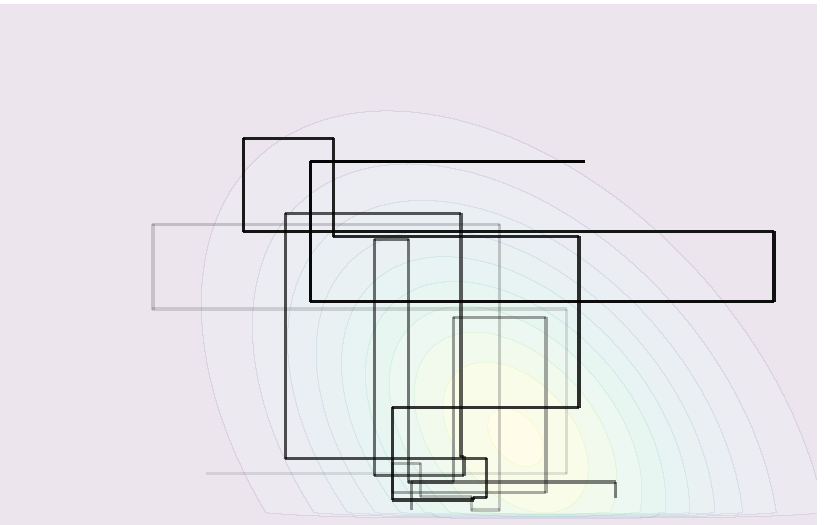
\includegraphics[keepaspectratio]{gibbs_files/figure-pdf/fig-Gibbs-steps-1.pdf}}

}

\caption{\label{fig-Gibbs-steps}Sampling trajectory for a bivariate
target using Gibbs sampling.}

\end{figure}%

As a toy illustration, we use Gibbs sampling to simulate data from a
\(d\)-dimensional multivariate Gaussian target with mean
\(\boldsymbol{\mu}\) and equicorrelation covariance matrix
\(\mathbf{\Sigma} = (1-\rho)\mathbf{I}_d + \rho\boldsymbol{1}_{d}\boldsymbol{1}^\top_d\)
with inverse
\[\mathbf{Q} = \boldsymbol{\Sigma}^{-1}=(1-\rho)^{-1}\left\{\mathbf{I}_d - \rho \mathbf{1}_d\mathbf{1}_d/(1+(d-1)\rho)\right\},\]
for known correlation coefficient \(\rho.\) While we can easily sample
independent observations, the exercise is insightful to see how well the
methods works as the dimension increases, and when the correlation
between pairs becomes stronger.

Consider
\(\boldsymbol{Y} \sim \mathsf{Gauss}_d(\boldsymbol{\mu}, \boldsymbol{\Sigma})\)
and a partition \((\boldsymbol{Y}_1^\top, \boldsymbol{Y}_2^\top)^\top\):
the conditional distribution of the \(k\) subvector \(\boldsymbol{Y}_1\)
given the \(d-k\) other components \(\boldsymbol{Y}_2\) is, in terms of
either the covariance (first line) or the precision (second line),
Gaussian where \begin{align*}
\boldsymbol{Y}_1 \mid \boldsymbol{Y}_2=\boldsymbol{y}_2 &\sim \mathsf{Gauss}_{k}\left\{ \boldsymbol{\mu}_1 + \boldsymbol{\Sigma}_{12} \boldsymbol{\Sigma}_{22}^{-1}(\boldsymbol{y}_2 - \boldsymbol{\mu}_2), \boldsymbol{\Sigma}_{11} - \boldsymbol{\Sigma}_{12}\boldsymbol{\Sigma}_{22}^{-1}\boldsymbol{\Sigma}_{21}\right\}
\\&\sim \mathsf{Gauss}_{k}\left\{ \boldsymbol{\mu}_1 -\mathbf{Q}_{11}^{-1}\mathbf{Q}_{12}(\boldsymbol{y}_2 - \boldsymbol{\mu}_2), \mathbf{Q}_{11}^{-1}\right\}.
\end{align*}

\begin{Shaded}
\begin{Highlighting}[]
\CommentTok{\# Create a 20 dimensional equicorrelation}
\NormalTok{d }\OtherTok{\textless{}{-}} \DecValTok{20}
\NormalTok{Q }\OtherTok{\textless{}{-}}\NormalTok{ hecbayes}\SpecialCharTok{::}\FunctionTok{equicorrelation}\NormalTok{(}\AttributeTok{d =}\NormalTok{ d, }\AttributeTok{rho =} \FloatTok{0.9}\NormalTok{, }\AttributeTok{precision =} \ConstantTok{TRUE}\NormalTok{)}
\NormalTok{B }\OtherTok{\textless{}{-}} \FloatTok{1e4}
\NormalTok{chains }\OtherTok{\textless{}{-}} \FunctionTok{matrix}\NormalTok{(}\DecValTok{0}\NormalTok{, }\AttributeTok{nrow =}\NormalTok{ B, }\AttributeTok{ncol =}\NormalTok{ d)}
\NormalTok{mu }\OtherTok{\textless{}{-}} \FunctionTok{rep}\NormalTok{(}\DecValTok{2}\NormalTok{, d)}
\CommentTok{\# Start far from mode}
\NormalTok{curr }\OtherTok{\textless{}{-}} \FunctionTok{rep}\NormalTok{(}\SpecialCharTok{{-}}\DecValTok{3}\NormalTok{, d)}
\ControlFlowTok{for}\NormalTok{(i }\ControlFlowTok{in} \FunctionTok{seq\_len}\NormalTok{(B))\{}
  \CommentTok{\# Random scan, updating one variable at a time}
  \ControlFlowTok{for}\NormalTok{(j }\ControlFlowTok{in} \FunctionTok{sample}\NormalTok{(}\DecValTok{1}\SpecialCharTok{:}\NormalTok{d, }\AttributeTok{size =}\NormalTok{ d))\{}
    \CommentTok{\# sample from conditional Gaussian given curr}
\NormalTok{    curr[j] }\OtherTok{\textless{}{-}}\NormalTok{ hecbayes}\SpecialCharTok{::}\FunctionTok{rcondmvnorm}\NormalTok{(}
      \AttributeTok{n =} \DecValTok{1}\NormalTok{,}
      \AttributeTok{value =}\NormalTok{ curr,}
      \AttributeTok{ind =}\NormalTok{ j,}
      \AttributeTok{mean =}\NormalTok{ mu,}
      \AttributeTok{precision =}\NormalTok{ Q)}
\NormalTok{  \}}
\NormalTok{  chains[i,] }\OtherTok{\textless{}{-}}\NormalTok{ curr }\CommentTok{\# save values after full round of update}
\NormalTok{\}}
\end{Highlighting}
\end{Shaded}

As the dimension of the parameter space increases, and as the
correlation between components becomes larger, the efficiency of the
Gibbs sampler degrades: Figure~\ref{fig-gibbs-normal} shows the first
component for updating one-parameter at a time for a multivariate
Gaussian target in dimensions \(d=20\) and \(d=3,\) started at four
deviation away from the mode. The chain makes smaller steps when there
is strong correlation, resulting in an inefficient sampler.

\begin{figure}[ht!]

\centering{

\pandocbounded{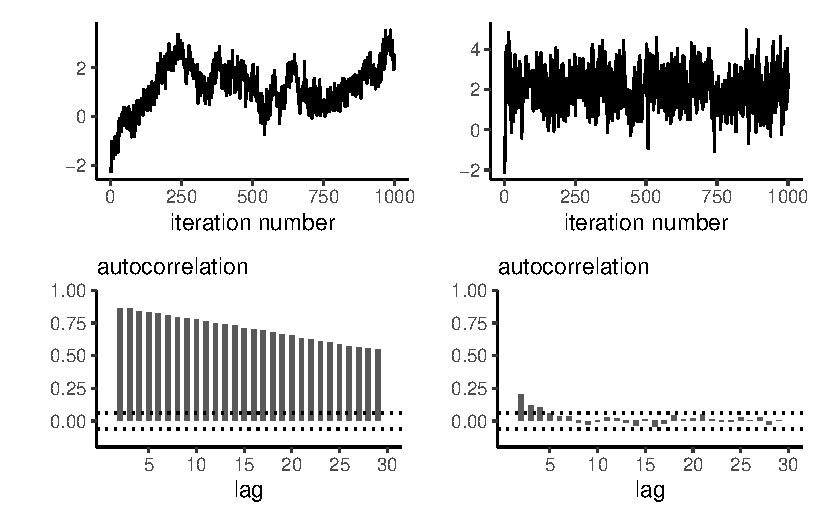
\includegraphics[keepaspectratio]{gibbs_files/figure-pdf/fig-gibbs-normal-1.pdf}}

}

\caption{\label{fig-gibbs-normal}Trace plots (top) and correlograms
(bottom) for the first component of a Gibbs sampler with \(d=20\)
equicorrelated Gaussian variates with correlation \(\rho=0.9\) (left)
and \(d=3\) with equicorrelation \(\rho=0.5\) (right).}

\end{figure}%

The main bottleneck in Gibbs sampling is determining all of the relevant
conditional distributions, which often relies on setting conditionally
conjugate priors. In large models with multiple layers, full
conditionals may only depend on a handful of parameters.

\begin{example}[]\protect\hypertarget{exm-gaussian-gamma}{}\label{exm-gaussian-gamma}

Consider a Gaussian model \(Y_i \sim \mathsf{Gauss}(\mu, \tau)\)
(\(i=1, \ldots, n\)) are independent, and where we assign priors
\(\mu \sim \mathsf{Gauss}(\nu, \omega)\) and
\(\tau \sim \mathsf{inv. gamma}(\alpha, \beta).\)

The joint posterior is not available in closed form, but the independent
priors for the mean and variance of the observations are conditionally
conjugate, since the joint posterior \begin{align*}
p(\mu, \tau \mid \boldsymbol{y}) \propto& \tau^{-n/2}\exp\left\{-\frac{1}{2\tau}\left(\sum_{i=1}^n y_i^2 - 2\mu \sum_{i=1}^n y_i+n\mu^2 \right)\right\}\\& \times \exp\left\{-\frac{(\mu-\nu)^2}{2\omega}\right\} \times \tau^{-\alpha-1}\exp(-\beta/\tau)
\end{align*} gives us \begin{align*}
p(\mu \mid \tau, \boldsymbol{y}) &\propto \exp\left\{-\frac{1}{2} \left( \frac{\mu^2-2\mu\overline{y}}{\tau/n} + \frac{\mu^2-2\nu \mu}{\omega}\right)\right\}\\
p(\tau \mid \mu, \boldsymbol{y}) & \propto \tau^{-n/2-\alpha-1}\exp\left[-\frac{1}{\tau}\left\{\frac{\sum_{i=1}^n (y_i-\mu)^2}{2} + \beta \right\}\right]
\end{align*} so we can simulate in turn \begin{align*}
\mu_t \mid \tau_{t-1}, \boldsymbol{y} &\sim \mathsf{Gauss}\left(\frac{n\overline{y}\omega+\tau \nu}{\tau + n\omega}, \frac{\omega \tau}{\tau + n\omega}\right)\\
\tau_t \mid \mu_t, \boldsymbol{y} &\sim \mathsf{inv. gamma}\left\{\frac{n}{2}+\alpha, \frac{\sum_{i=1}^n (y_i-\mu)^2}{2} + \beta\right\}.
\end{align*}

\end{example}

\begin{remark}[Gibbs sampler and proper posterior]
Gibbs sampling cannot be used to determine if the posterior is improper.
If the posterior is not well defined, the Markov chains may seem to
stabilize even though there is no proper target.
\end{remark}

\section{Data augmentation and auxiliary variables}\label{sec-gibbs-da}

In many problems, the likelihood
\(p(\boldsymbol{y}; \boldsymbol{\theta})\) is intractable or costly to
evaluate and auxiliary variables are introduced to simplify
calculations, as in the expectation-maximization algorithm. The Bayesian
analog is data augmentation (\citeproc{ref-Tanner.Wong:1987}{Tanner and
Wong 1987}), which we present succinctly: let
\(\boldsymbol{\theta} \in \Theta\) be a vector of parameters and
consider auxiliary variables \(\boldsymbol{u} \in \mathbb{R}^k\) such
that
\(\int_{\mathbb{R}^k} p(\boldsymbol{u}, \boldsymbol{\theta}; \boldsymbol{y}) \mathrm{d} \boldsymbol{u} = p(\boldsymbol{\theta}; \boldsymbol{y}),\)
i.e., the marginal distribution is that of interest, but evaluation of
\(p(\boldsymbol{u}, \boldsymbol{\theta}; \boldsymbol{y})\) is cheaper.
The data augmentation algorithm consists in running a Markov chain on
the augmented state space \((\Theta, \mathbb{R}^k),\) simulating in turn
from the conditionals
\(p(\boldsymbol{u}; \boldsymbol{\theta}, \boldsymbol{y})\) and
\(p(\boldsymbol{\theta}; \boldsymbol{u}, \boldsymbol{y})\) with new
variables chosen to simplify the likelihood. If simulation from the
conditionals is straightforward, we can also use data augmentation to
speed up calculations or improve mixing. For more details and examples,
see Dyk and Meng (\citeproc{ref-vanDyk.Meng:2001}{2001}) and Hobert
(\citeproc{ref-Hobert:2011}{2011}).

\begin{example}[Probit
regression]\protect\hypertarget{exm-probit-regression}{}\label{exm-probit-regression}

Consider binary responses \(\boldsymbol{Y}_i,\) for which we postulate a
probit regression model, \begin{align*}
p_i = \Pr(Y_i=1) = \Phi(\beta_0 + \beta_1 \mathrm{X}_{i1} + \cdots + \beta_p\mathrm{X}_{ip}),
\end{align*} where \(\Phi\) is the distribution function of the standard
Gaussian distribution. The likelihood of the probit model for a sample
of \(n\) independent observations is
\[L(\boldsymbol{\beta}; \boldsymbol{y}) = \prod_{i=1}^n p_i^{y_i}(1-p_i)^{1-y_i},\]
and this prevents easy simulation. We can consider a data augmentation
scheme where \(Y_i = \mathsf{I}(Z_i > 0),\) where
\(Z_i \sim \mathsf{Gauss}(\mathbf{x}_i\boldsymbol{\beta}, 1),\) with
\(\mathbf{x}_i\) denoting the \(i\)th row of the design matrix.

The augmented data likelihood is \begin{align*}
p(\boldsymbol{z}, \boldsymbol{y} \mid \boldsymbol{\beta}) \propto \exp\left\{-\frac{1}{2}(\boldsymbol{z} - \mathbf{X}\boldsymbol{\beta})^\top(\boldsymbol{z} - \mathbf{X}\boldsymbol{\beta})\right\} \times \prod_{i=1}^n \mathsf{I}(z_i > 0)^{y_i}\mathsf{I}(z_i \le 0)^{1-y_i}
\end{align*} Given \(Z_i,\) the coefficients \(\boldsymbol{\beta}\) are
simply the results of ordinary linear regression with unit variance, so
\begin{align*}
\boldsymbol{\beta} \mid \boldsymbol{z}, \boldsymbol{y} &\sim \mathsf{Gauss}\left\{\widehat{\boldsymbol{\beta}}, (\mathbf{X}^\top\mathbf{X})^{-1}\right\}
\end{align*} with
\(\widehat{\boldsymbol{\beta}}=(\mathbf{X}^\top\mathbf{X})^{-1}\mathbf{X}^\top\boldsymbol{z}\)
is the ordinary least square estimator from the regression with model
matrix \(\mathbf{X}\) and response vector \(\boldsymbol{z}.\) The
augmented variables \(Z_i\) are conditionally independent and truncated
Gaussian with \begin{align*}
Z_i \mid y_i, \boldsymbol{\beta} \sim \begin{cases}
\mathsf{trunc. Gauss}(\mathbf{x}_i\boldsymbol{\beta}, -\infty, 0) & y_i =0 \\
\mathsf{trunc. Gauss}(\mathbf{x}_i\boldsymbol{\beta}, 0, \infty) & y_i =1.
\end{cases}
\end{align*} and we can use the algorithms of
Example~\ref{exm-accept-reject-truncated} to simulate these.

\begin{Shaded}
\begin{Highlighting}[]
\NormalTok{probit\_regression }\OtherTok{\textless{}{-}} \ControlFlowTok{function}\NormalTok{(y, x, }\AttributeTok{B =} \FloatTok{1e4}\NormalTok{L, }\AttributeTok{burnin =} \DecValTok{100}\NormalTok{)\{}
\NormalTok{  y }\OtherTok{\textless{}{-}} \FunctionTok{as.numeric}\NormalTok{(y)}
\NormalTok{  n }\OtherTok{\textless{}{-}} \FunctionTok{length}\NormalTok{(y)}
  \CommentTok{\# Add intercept}
\NormalTok{  x }\OtherTok{\textless{}{-}} \FunctionTok{cbind}\NormalTok{(}\DecValTok{1}\NormalTok{, }\FunctionTok{as.matrix}\NormalTok{(x))}
\NormalTok{  xtxinv }\OtherTok{\textless{}{-}} \FunctionTok{solve}\NormalTok{(}\FunctionTok{crossprod}\NormalTok{(x))}
  \CommentTok{\# Use MLE as initial values}
\NormalTok{  beta.curr }\OtherTok{\textless{}{-}} \FunctionTok{coef}\NormalTok{(}\FunctionTok{glm}\NormalTok{(y }\SpecialCharTok{\textasciitilde{}}\NormalTok{ x }\SpecialCharTok{{-}} \DecValTok{1}\NormalTok{, }\AttributeTok{family=}\FunctionTok{binomial}\NormalTok{(}\AttributeTok{link =} \StringTok{"probit"}\NormalTok{)))}
  \CommentTok{\# Containers}
\NormalTok{  Z }\OtherTok{\textless{}{-}} \FunctionTok{rep}\NormalTok{(}\DecValTok{0}\NormalTok{, n)}
\NormalTok{  chains }\OtherTok{\textless{}{-}} \FunctionTok{matrix}\NormalTok{(}\DecValTok{0}\NormalTok{, }\AttributeTok{nrow =}\NormalTok{ B, }\AttributeTok{ncol =} \FunctionTok{length}\NormalTok{(beta.curr))}
  \ControlFlowTok{for}\NormalTok{(b }\ControlFlowTok{in} \FunctionTok{seq\_len}\NormalTok{(B }\SpecialCharTok{+}\NormalTok{ burnin))\{}
\NormalTok{    ind }\OtherTok{\textless{}{-}} \FunctionTok{max}\NormalTok{(}\DecValTok{1}\NormalTok{, b }\SpecialCharTok{{-}}\NormalTok{ burnin)}
\NormalTok{    Z }\OtherTok{\textless{}{-}}\NormalTok{ TruncatedNormal}\SpecialCharTok{::}\FunctionTok{rtnorm}\NormalTok{(}
      \AttributeTok{n =} \DecValTok{1}\NormalTok{,}
      \AttributeTok{mu =} \FunctionTok{as.numeric}\NormalTok{(x }\SpecialCharTok{\%*\%}\NormalTok{ beta.curr),}
      \AttributeTok{lb =} \FunctionTok{ifelse}\NormalTok{(y }\SpecialCharTok{==} \DecValTok{0}\NormalTok{, }\SpecialCharTok{{-}}\ConstantTok{Inf}\NormalTok{, }\DecValTok{0}\NormalTok{),}
      \AttributeTok{ub =} \FunctionTok{ifelse}\NormalTok{(y }\SpecialCharTok{==} \DecValTok{1}\NormalTok{, }\ConstantTok{Inf}\NormalTok{, }\DecValTok{0}\NormalTok{),}
      \AttributeTok{sd =} \DecValTok{1}\NormalTok{)}
\NormalTok{    beta.curr }\OtherTok{\textless{}{-}}\NormalTok{ chains[ind,] }\OtherTok{\textless{}{-}} \FunctionTok{as.numeric}\NormalTok{(}
\NormalTok{      mvtnorm}\SpecialCharTok{::}\FunctionTok{rmvnorm}\NormalTok{(}
        \AttributeTok{n =} \DecValTok{1}\NormalTok{,}
        \AttributeTok{mean =} \FunctionTok{coef}\NormalTok{(}\FunctionTok{lm}\NormalTok{(Z }\SpecialCharTok{\textasciitilde{}}\NormalTok{ x }\SpecialCharTok{{-}} \DecValTok{1}\NormalTok{)),}
        \AttributeTok{sigma =}\NormalTok{ xtxinv))}
\NormalTok{  \}}
\FunctionTok{return}\NormalTok{(chains)}
\NormalTok{\}}
\end{Highlighting}
\end{Shaded}

\end{example}

\begin{example}[Bayesian
LASSO]\protect\hypertarget{exm-student-mixture-gaussian}{}\label{exm-student-mixture-gaussian}

The Laplace distribution with location \(\mu\) and scale \(\sigma,\) has
density \begin{align*}
f(x; \mu, \sigma) = \frac{1}{2\sigma}\exp\left(-\frac{|x-\mu|}{\sigma}\right).
\end{align*} It can be expressed as a scale mixture of Gaussians, where
\(Y_i \sim \mathsf{Laplace}(\mu, \sigma)\) is equivalent to
\(Z_i \mid \tau \sim \mathsf{Gauss}(\mu, \lambda_i)\) and
\(\Lambda_i \sim \mathsf{expo}\{(2\sigma^2)^{-1}\}.\) To see this, we
first look at the Wald (or inverse Gaussian) distribution
\(\mathsf{Wald}(\nu, \omega)\) with location \(\nu >0\) and shape
\(\omega>0,\), whose density is \begin{align*}
f(y; \nu, \omega) &= \left(\frac{\omega}{2\pi y^{3}}\right)^{1/2} \exp\left\{ - \frac{\omega (y-\nu)^2}{2\nu^2y}\right\}, \quad y > 0
\\ &\stackrel{y}{\propto} y^{-3/2}\exp\left\{-\frac{\omega}{2} \left(\frac{y}{\nu^2} + \frac{1}{y}\right)\right\}
\end{align*} To show that the marginal (unconditionally) is Laplace, we
write the joint density and integrate out the variance term \(\lambda,\)
make the change of variable to get the result in terms of the precision
\(\xi = 1/\lambda\), whence \begin{align*}
p(z) &= \int_{0}^{\infty} p(z \mid \lambda) p(\lambda) \mathrm{d} \lambda 
\\&= \int_0^{\infty} \frac{1}{(2\pi\lambda)^{1/2}}\exp \left\{-\frac{1}{2\lambda}(z-\mu)^2\right\}\frac{1}{2\sigma^2}\exp\left(-\frac{\lambda}{2\sigma^2}\right)  \mathrm{d} \lambda 
\\&= \frac{1}{2\sigma^2}\int_0^{\infty} \frac{1}{(2\pi\lambda)^{1/2}}\exp \left[-\frac{1}{2} \left\{\frac{(z-\mu)^2}{\lambda}+\frac{\lambda}{\sigma^2}\right\}\right] \mathrm{d} \lambda 
\\&= \frac{1}{2\sigma^2}\int_0^{\infty} \frac{1}{\xi^2}\frac{\xi^{1/2}}{(2\pi)^{1/2}}\exp \left[-\frac{1}{2\sigma^2} \left\{\xi\sigma^2(z-\mu)^2+\frac{1}{\xi}\right\}\right] \mathrm{d} \xi
\\&= \frac{1}{2\sigma^2}\int_0^{\infty} \frac{1}{(2\pi\xi^3)^{1/2}}\exp \left[-\frac{\omega}{2} \left\{\frac{\xi}{\nu^2}+\frac{1}{\xi}\right\}\right] \mathrm{d} \xi
\\&= \frac{1}{2\sigma^2\omega^{1/2}}\exp\left(-\frac{\omega}{\nu}\right) 
\\& = \frac{1}{2\sigma}\exp\left(-\frac{|z-\mu|}{\sigma}\right).
\end{align*} upon recovering the conditional density of
\(\Xi \mid Z \sim \mathsf{Wald}(\nu, \omega)\) with parameters
\(\nu=(\sigma|z-\mu|)^{-1}\) and \(\omega=\sigma^{-2}\).

Park and Casella (\citeproc{ref-Park.Casella:2008}{2008}) use this
hierarchical construction to define the Bayesian LASSO. With a model
matrix \(\mathbf{X}\) whose columns are standardized to have mean zero
and unit standard deviation, we may write \begin{align*}
\boldsymbol{Y} \mid \mu, \boldsymbol{\beta}, \sigma^2 &\sim  \mathsf{Gauss}_n(\mu \boldsymbol{1}_n + \mathbf{X}\boldsymbol{\beta}, \sigma^2 \mathbf{I}_n)\\
\beta_j \mid \sigma^2, \tau_j &\sim \mathsf{Gauss}(0, \sigma^2\tau_j)\\
\tau_j &\sim \mathsf{expo}(\lambda/2)
\end{align*} With the improper prior
\(p(\mu, \sigma^2) \propto 1/\sigma^2\) and with \(n\) independent and
identically distributed Laplace variates, written as a scale mixture,
the model is amenable to Gibbs sampling. With
\(\mathbf{D}^{-1}_{\tau} = \mathrm{diag}(\tau_1^{-1}, \ldots, \tau_p^{-1})\)
and
\(\tilde{\boldsymbol{y}} = \boldsymbol{y} - \overline{y}\mathbf{1}_n\)
the centered response vector, we can simulate in turn
(\citeproc{ref-Park.Casella:2008}{Park and Casella 2008}) \begin{align*}
\mu \mid \sigma^2, \boldsymbol{y} &\sim \mathsf{Gauss}(\overline{y}, \sigma^2/n) \\
\boldsymbol{\beta} \mid \sigma^2, \boldsymbol{\tau}, \boldsymbol{y} &\sim \mathsf{Gauss}_p\left\{\left(\mathbf{X}^\top\mathbf{X} + \mathbf{D}^{-1}_{\tau}\right)^{-1} \mathbf{X}\widetilde{\boldsymbol{y}}, \sigma^2\left(\mathbf{X}^\top\mathbf{X} + \mathbf{D}^{-1}_{\tau}\right)^{-1}\right\}\\
\sigma^2 \mid \boldsymbol{\beta}, \boldsymbol{\tau},\boldsymbol{y} &\sim \mathsf{inv. gamma}\left\{ \frac{n-1+p}{2}, \frac{(\widetilde{\boldsymbol{y}}-\mathbf{X}\boldsymbol{\beta})^\top(\widetilde{\boldsymbol{y}}-\mathbf{X}\boldsymbol{\beta}) + \boldsymbol{\beta}^\top\mathbf{D}^{-1}_{\tau} \boldsymbol{\beta}}{2}\right\},\\
\tau_j^{-1} \mid \boldsymbol{\beta}, \sigma^2 &\sim \mathsf{Wald} \left( \frac{\lambda^{1/2}\sigma}{|\beta_j|}, \lambda\right)
\end{align*} where the last three conditional distributions follow from
marginalizing out \(\mu.\)

The Bayesian LASSO places a Laplace penalty on the regression
coefficients, with lower values of \(\lambda\) yielding more shrinkage.
Figure~\ref{fig-lasso-traceplot} shows a replication of Figure 1 of Park
and Casella (\citeproc{ref-Park.Casella:2008}{2008}), fitted to the
\texttt{diabetes} data. Note that, contrary to the frequentist setting,
none of the posterior draws of \(\boldsymbol{\beta}\) are exactly zero.

\begin{figure}[ht!]

\centering{

\pandocbounded{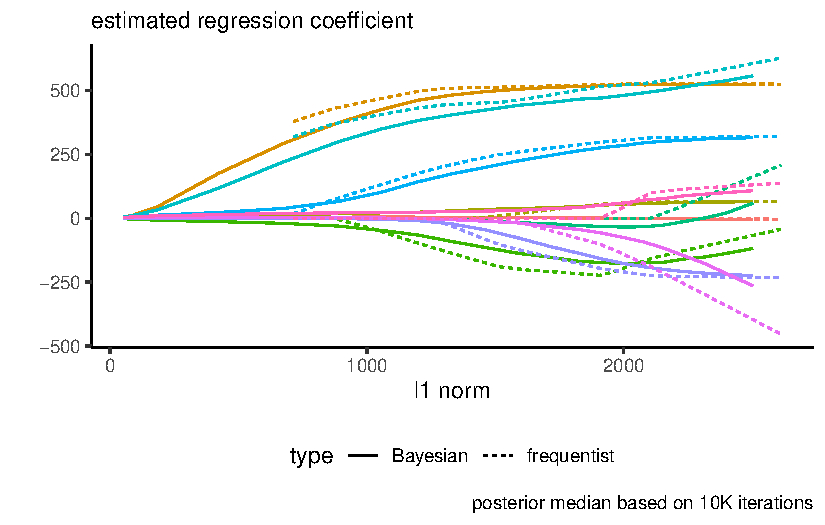
\includegraphics[keepaspectratio]{gibbs_files/figure-pdf/fig-lasso-traceplot-1.pdf}}

}

\caption{\label{fig-lasso-traceplot}Traceplot of \(\beta\) coefficients
(penalized maximum likelihood estimates and median aposteriori as a
function of the \(l_1\) norm of the coefficients, with lower values of
the latter corresponding to higher values of the penalty \(\lambda.\)}

\end{figure}%

Many elliptical distributions can be cast as scale mixture models of
spherical or Gaussian variables; see, e.g., Section 10.2 of Albert
(\citeproc{ref-Albert:2009}{2009}) for a similar derivation with a
Student-\(t\) distribution.

\end{example}

\begin{example}[Mixture
models]\protect\hypertarget{exm-mixture}{}\label{exm-mixture}

In clustering problems, we can specify that observations arise from a
mixture model with a fixed or unknown number of coefficients: the
interest lies then in estimating the relative weights of the components,
and their location and scale.

A \(K\)-mixture model is a weighted combination of models frequently
used in clustering or to model subpopulations with respective densities
\(f_k,\) with density
\[f(x; \boldsymbol{\theta}, \boldsymbol{\omega}) = \sum_{k=1}^K \omega_kf_k(x; \boldsymbol{\theta}_k), \qquad \omega_1 + \cdots \omega_K=1.\]
Since the density involves a sum, numerical optimization is challenging.
Let \(C_i\) denote the cluster index for observation \(i\): if we knew
the value of \(C_i =j,\) the density would involve only \(f_j.\) We can
thus use latent variables representing the group allocation to simplify
the problem and run an EM algorithm or use the data augmentation. In an
iterative framework, we can consider the complete data as the tuples
\((X_i, Z_i),\) where \(Z_i = \mathsf{I}(C_i=k).\)

With the augmented data, the likelihood becomes \begin{align*}
\prod_{i=1}^n \prod_{k=1}^K \{\omega_kf_k(x; \boldsymbol{\theta}_k)\}^{Z_i},
\end{align*} so the conditional distribution of
\(Z_i \mid X_i, \boldsymbol{\omega}, \boldsymbol{\theta} \sim \mathsf{multinom}(1, \boldsymbol{\gamma}_{ik})\)
where
\[\gamma_{ik} = \frac{\omega_k f_k(X_i\boldsymbol{\theta}_k)}{\sum_{j=1}^K \omega_jf_j(X_i\boldsymbol{\theta}_k)}.\]
Given suitable priors for the probabilities \(\boldsymbol{\omega}\) and
\(\boldsymbol{\theta} \equiv \{\boldsymbol{\theta}_1, \ldots, \boldsymbol{\theta}_k\},\)
we can use Gibbs sampling updating \(\boldsymbol{Z},\)
\(\boldsymbol{\omega}\) and \(\boldsymbol{\theta}\) in turn, assigning a
conjugate Dirichlet prior for \(\boldsymbol{\omega}.\)

\end{example}

\begin{example}[Mixture model for
geyser]\protect\hypertarget{exm-mixture-model}{}\label{exm-mixture-model}

We consider a Gaussian mixture model for waiting time between two
eruptions of the Old Faithful geyser in Yellowstone. The distribution is
of the form \begin{align*}
f_i(x) = p_i \phi_{1}(x_i; \mu_1, \tau_1^{-1}) + (1-p_i)\phi_{2}(x_i; \mu_2, \tau_2^{-1}).
\end{align*} where \(\phi(\cdot; \mu, \tau^{-1})\) is the density
function of a Gaussian with mean \(\mu\) and precision \(\tau.\) We
assign conjugate priors with \(p_i \sim \mathsf{beta}(a_1, a_2),\)
\(\mu_j \sim \mathsf{Gauss}(c, d^{-1})\) and
\(\tau_j \sim \mathsf{gamma}(b_1, b_2).\) For the hyperpriors, we use
\(a_1=a_2=1,\) \(b_1=1, b_2 = 0.1,\) \(c = 60,\) and \(d = 1/40.\)

\begin{Shaded}
\begin{Highlighting}[]
\FunctionTok{data}\NormalTok{(faithful)}
\NormalTok{n }\OtherTok{\textless{}{-}} \FunctionTok{nrow}\NormalTok{(faithful)}
\NormalTok{y }\OtherTok{\textless{}{-}}\NormalTok{ faithful}\SpecialCharTok{$}\NormalTok{waiting}
\CommentTok{\# Fix hyperpriors}
\NormalTok{a1 }\OtherTok{\textless{}{-}} \DecValTok{2}\NormalTok{; a2 }\OtherTok{\textless{}{-}} \DecValTok{2}\NormalTok{; c }\OtherTok{\textless{}{-}} \DecValTok{60}\NormalTok{; d }\OtherTok{\textless{}{-}} \DecValTok{1}\SpecialCharTok{/}\DecValTok{40}\NormalTok{; b1 }\OtherTok{\textless{}{-}} \DecValTok{1}\NormalTok{; b2 }\OtherTok{\textless{}{-}} \FloatTok{0.01}
\CommentTok{\# Assign observations at random to groups}
\FunctionTok{set.seed}\NormalTok{(}\DecValTok{80601}\NormalTok{)}
\NormalTok{cut }\OtherTok{\textless{}{-}} \FunctionTok{runif}\NormalTok{(}\DecValTok{1}\NormalTok{, }\FloatTok{0.1}\NormalTok{, }\FloatTok{0.9}\NormalTok{)}\SpecialCharTok{*}\FunctionTok{diff}\NormalTok{(}\FunctionTok{range}\NormalTok{(y)) }\SpecialCharTok{+} \FunctionTok{min}\NormalTok{(y)}
\NormalTok{group }\OtherTok{\textless{}{-}} \FunctionTok{as.integer}\NormalTok{(y }\SpecialCharTok{\textgreater{}}\NormalTok{ cut)}
\NormalTok{p }\OtherTok{\textless{}{-}} \FunctionTok{sum}\NormalTok{(group }\SpecialCharTok{==} \DecValTok{0}\NormalTok{L)}\SpecialCharTok{/}\NormalTok{n}
\NormalTok{mu }\OtherTok{\textless{}{-}} \FunctionTok{c}\NormalTok{(}\FunctionTok{mean}\NormalTok{(y[group }\SpecialCharTok{==} \DecValTok{0}\NormalTok{]), }\FunctionTok{mean}\NormalTok{(y[group }\SpecialCharTok{==} \DecValTok{1}\NormalTok{]))}
\NormalTok{prec }\OtherTok{\textless{}{-}} \DecValTok{1}\SpecialCharTok{/}\FunctionTok{c}\NormalTok{(}\FunctionTok{var}\NormalTok{(y[group }\SpecialCharTok{==} \DecValTok{0}\NormalTok{]), }\FunctionTok{var}\NormalTok{(y[group }\SpecialCharTok{==} \DecValTok{1}\NormalTok{]))}
\CommentTok{\# Storage and number of replications}
\NormalTok{B }\OtherTok{\textless{}{-}} \FloatTok{1e4}\NormalTok{L}
\NormalTok{theta }\OtherTok{\textless{}{-}} \FunctionTok{matrix}\NormalTok{(}\AttributeTok{nrow =}\NormalTok{ B, }\AttributeTok{ncol =} \DecValTok{5}\NormalTok{L)}
\CommentTok{\# Step 1: assign variables to clusters}
\ControlFlowTok{for}\NormalTok{(b }\ControlFlowTok{in} \DecValTok{1}\SpecialCharTok{:}\NormalTok{B)\{}
\NormalTok{  d1 }\OtherTok{\textless{}{-}} \FunctionTok{dnorm}\NormalTok{(y, }\AttributeTok{mean =}\NormalTok{ mu[}\DecValTok{1}\NormalTok{], }\AttributeTok{sd =} \DecValTok{1}\SpecialCharTok{/}\FunctionTok{sqrt}\NormalTok{(prec[}\DecValTok{1}\NormalTok{])) }\CommentTok{\# group 0 }
\NormalTok{  d2 }\OtherTok{\textless{}{-}} \FunctionTok{dnorm}\NormalTok{(y, }\AttributeTok{mean =}\NormalTok{ mu[}\DecValTok{2}\NormalTok{], }\AttributeTok{sd =} \DecValTok{1}\SpecialCharTok{/}\FunctionTok{sqrt}\NormalTok{(prec[}\DecValTok{2}\NormalTok{])) }\CommentTok{\# group 1}
  \CommentTok{\# Data augmentation: group labels}
\NormalTok{  group }\OtherTok{\textless{}{-}} \FunctionTok{rbinom}\NormalTok{(}\AttributeTok{n =}\NormalTok{ n, }\AttributeTok{size =} \FunctionTok{rep}\NormalTok{(}\DecValTok{1}\NormalTok{, n), }\AttributeTok{prob =}\NormalTok{ (}\DecValTok{1}\SpecialCharTok{{-}}\NormalTok{p)}\SpecialCharTok{*}\NormalTok{d2}\SpecialCharTok{/}\NormalTok{(p}\SpecialCharTok{*}\NormalTok{d1 }\SpecialCharTok{+}\NormalTok{ (}\DecValTok{1}\SpecialCharTok{{-}}\NormalTok{p)}\SpecialCharTok{*}\NormalTok{d2))}
  \CommentTok{\# Step 2: update probability of cluster}
\NormalTok{  p }\OtherTok{\textless{}{-}} \FunctionTok{rbeta}\NormalTok{(}\AttributeTok{n =} \DecValTok{1}\NormalTok{, }\AttributeTok{shape1 =}\NormalTok{ n }\SpecialCharTok{{-}} \FunctionTok{sum}\NormalTok{(group) }\SpecialCharTok{+}\NormalTok{ a1, }\FunctionTok{sum}\NormalTok{(group) }\SpecialCharTok{+}\NormalTok{ a2)}
  \ControlFlowTok{for}\NormalTok{(j }\ControlFlowTok{in} \DecValTok{1}\SpecialCharTok{:}\DecValTok{2}\NormalTok{)\{}
\NormalTok{    yg }\OtherTok{\textless{}{-}}\NormalTok{ y[group }\SpecialCharTok{==}\NormalTok{ (j}\DecValTok{{-}1}\NormalTok{L)]}
\NormalTok{    ng }\OtherTok{\textless{}{-}} \FunctionTok{length}\NormalTok{(yg)}
\NormalTok{    prec\_mu }\OtherTok{\textless{}{-}}\NormalTok{ prec[j] }\SpecialCharTok{*}\NormalTok{ ng }\SpecialCharTok{+}\NormalTok{ d}
\NormalTok{    mean\_mu }\OtherTok{\textless{}{-}}\NormalTok{ (}\FunctionTok{sum}\NormalTok{(yg)}\SpecialCharTok{*}\NormalTok{prec[j] }\SpecialCharTok{+}\NormalTok{ c}\SpecialCharTok{*}\NormalTok{d)}\SpecialCharTok{/}\NormalTok{prec\_mu}
\NormalTok{    mu[j] }\OtherTok{\textless{}{-}} \FunctionTok{rnorm}\NormalTok{(}\AttributeTok{n =} \DecValTok{1}\NormalTok{, }\AttributeTok{mean =}\NormalTok{ mean\_mu, }\AttributeTok{sd =} \DecValTok{1}\SpecialCharTok{/}\FunctionTok{sqrt}\NormalTok{(prec\_mu))}
\NormalTok{    prec[j] }\OtherTok{\textless{}{-}} \FunctionTok{rgamma}\NormalTok{(}\AttributeTok{n =} \DecValTok{1}\NormalTok{, }
                      \AttributeTok{shape =}\NormalTok{ b1 }\SpecialCharTok{+}\NormalTok{ ng}\SpecialCharTok{/}\DecValTok{2}\NormalTok{, }
                      \AttributeTok{rate =}\NormalTok{ b2 }\SpecialCharTok{+} \FloatTok{0.5}\SpecialCharTok{*}\FunctionTok{sum}\NormalTok{((yg}\SpecialCharTok{{-}}\NormalTok{mu[j])}\SpecialCharTok{\^{}}\DecValTok{2}\NormalTok{))}
\NormalTok{  \}}
\NormalTok{  theta[b, ] }\OtherTok{\textless{}{-}} \FunctionTok{c}\NormalTok{(p, mu, prec)}
\NormalTok{\}}
\CommentTok{\# Discard initial observations (burn in)}
\NormalTok{theta }\OtherTok{\textless{}{-}}\NormalTok{ theta[}\SpecialCharTok{{-}}\NormalTok{(}\DecValTok{1}\SpecialCharTok{:}\DecValTok{100}\NormalTok{),]}
\end{Highlighting}
\end{Shaded}

\begin{figure}[ht!]

\centering{

\pandocbounded{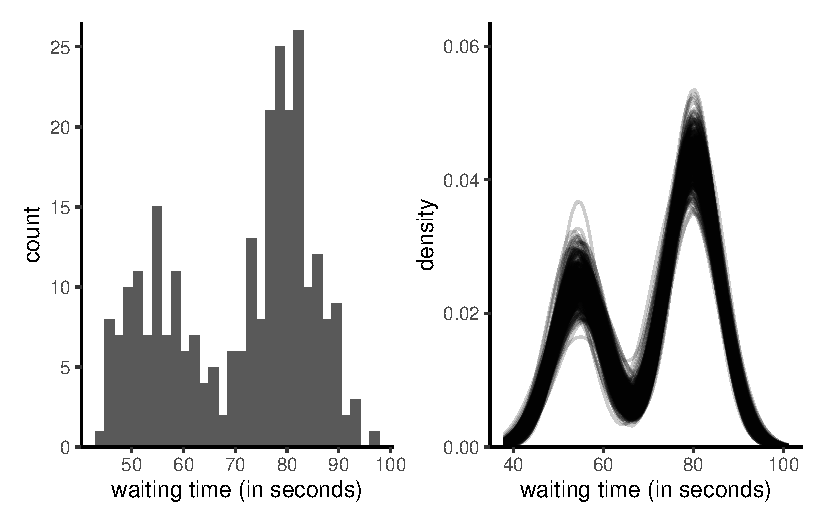
\includegraphics[keepaspectratio]{gibbs_files/figure-pdf/fig-density-mixt-1.pdf}}

}

\caption{\label{fig-density-mixt}One-dimensional density mixture for the
Old Faithful data, with histogram of data (left) and posterior density
draws (right).}

\end{figure}%

\end{example}

\begin{refremark}[Label switching in mixture models]
If we run a MCMC algorithm to sample from a mixture models, the
likelihood is invariant to permutation of the group labels, leading to
identifiability issues when the chain swaps modes, when running multiple
Markov chains with symmetric priors or using tempering algorithms. Two
chains may thus reach the same stationary distribution, with group
labels swapped. It is sometimes necessary to impose ordering constraints
on the mean parameters \(\boldsymbol{\mu},\) although this isn't
necessarily easy to generalize beyond the univariate setting. See Jasra,
Holmes, and Stephens (\citeproc{ref-Jasra.Holmes.Stephens:2005}{2005})
and Stephens (\citeproc{ref-Stephens:2002}{2002}) for more details.

\label{rem-label-switching}

\end{refremark}

\begin{tcolorbox}[enhanced jigsaw, colframe=quarto-callout-important-color-frame, colback=white, leftrule=.75mm, opacitybacktitle=0.6, toprule=.15mm, colbacktitle=quarto-callout-important-color!10!white, title=\textcolor{quarto-callout-important-color}{\faExclamation}\hspace{0.5em}{\textbf{Summary}:}, left=2mm, breakable, titlerule=0mm, bottomrule=.15mm, opacityback=0, bottomtitle=1mm, rightrule=.15mm, arc=.35mm, toptitle=1mm, coltitle=black]

\begin{itemize}
\tightlist
\item
  Gibbs sampling is a special case of Metropolis--Hastings algorithm,
  where we sample from the conditional distributions given other
  parameters.
\item
  Use of (conditionally) conjugate priors enables Gibbs sampling.
\item
  The fact that any Gibbs step is accepted with probability one does not
  mean the sampler is efficient: there can be significant
  autocorrelation in the chains.
\item
  We can sometimes update parameters jointly, or reduce the dependence
  by integrating out some of the conditioning variables
  (marginalization).
\item
  We can use Gibbs step for some updates within a more general
  algorithm.
\item
  Even if there is no closed-form expression, we can use Monte Carlo
  methods to simulate parameters in a Gibbs sampler.
\item
  In many scenarios, the likelihood is costly to evaluate or not
  amenable to Gibbs sampling. Data augmentation introduces additional
  parameters to the model in exchange for simplifying the likelihood.
\item
  Data augmentation leads to a trade-off between complexity and
  efficiency (more parameters, slower mixing).
\item
  Data augmentation is commonly used for expectation-maximisation (EM)
  algorithm for maximum likelihood estimation in frequentist setting.
\item
  Special classes of models (Bayesian linear regression, mixtures, etc.)
  are typically fitted using Gibbs sampling.
\item
  Probabilistic programming languages (Bugs, JAGS) rely on Gibbs
  sampling.
\end{itemize}

\end{tcolorbox}

\bookmarksetup{startatroot}

\chapter{Computational strategies and
diagnostics}\label{computational-strategies-and-diagnostics}

The Bayesian workflow is a coherent framework for model formulation
construction, inference and validation. It typically involves trying and
comparing different models, adapting and modifying these models
(\citeproc{ref-Gelman:2020}{Gelman et al. 2020}); see also
\href{https://betanalpha.github.io/assets/case_studies/principled_bayesian_workflow.html}{Michael
Betancourt} for excellent visualizations. In this chapter, we focus on
three aspects of the workflow: model validation, evaluation and
comparison.

\begin{tcolorbox}[enhanced jigsaw, colframe=quarto-callout-important-color-frame, colback=white, leftrule=.75mm, opacitybacktitle=0.6, toprule=.15mm, colbacktitle=quarto-callout-important-color!10!white, title=\textcolor{quarto-callout-important-color}{\faExclamation}\hspace{0.5em}{\textbf{Learning objectives}:}, left=2mm, breakable, titlerule=0mm, bottomrule=.15mm, opacityback=0, bottomtitle=1mm, rightrule=.15mm, arc=.35mm, toptitle=1mm, coltitle=black]

At the end of the chapter, students should be able to

\begin{itemize}
\tightlist
\item
  use output of MCMC to obtain estimates and standard errors.
\item
  choose suitable test statistics to evaluate model adequacy.
\item
  assess convergence using graphical tools and effective sample size.
\item
  perform model comparisons using Bayes factor or predictive measures.
\item
  diagnose performance of MCMC algorithms (in terms of mixing and
  effective sample size).
\item
  implement strategies to improve sampling performance, including block
  updates, reparametrization and marginalization.
\end{itemize}

\end{tcolorbox}

For a given problem, there are many different Markov chain Monte Carlo
algorithms that one can implement: they will typically be distinguished
based on the running time per iteration and the efficiency of the
samplers, with algorithms providing realizations of Markov chains with
lower autocorrelation being preferred. Many visual diagnostics and
standard tests can be used to diagnose lack of convergence, or
inefficiency. The purpose of this section is to review these in turn,
and to go over tricks that can improve mixing.

\textbf{Generating artificial data}: Some problems and checks relate to
models and the correct implementations (of the algorithms). Sometimes,
the probabilistic procedure will generate draws, but it's unclear
whether our numerical implementation is correct. We can sometimes see
this if the output is truly misleading, but it's not always obvious. We
can for example generate an ``artificial'' or fake data set from the
model with some fixed parameter inputs to see if we can recover the
parameter values used to generate these within some credible set.

Many such sanity checks can be implemented by means of simulations.
Consider prior predictive checks: if the prior has a distribution from
which we can generate, we can obtain prior draws from
\(p(\boldsymbol{\theta})\), generate data from the prior predictive
\(p(y \mid \boldsymbol{\theta})\) by simulating new observations from
the data generating mechanism of the likelihood, and use these to obtain
prior predictive by removing the likelihood component altogether: the
draws from the prior predictive should then match posterior draws with
only the prior.

The ``data-averaged posterior'' is obtained upon noting that
(\citeproc{ref-Geweke:2004}{Geweke 2004}) \begin{align*}
p(\boldsymbol{\theta}) = \int \int_{\boldsymbol{\Theta}} p( \boldsymbol{\theta} \mid \boldsymbol{y}) p(\boldsymbol{y} \mid \widetilde{\boldsymbol{\theta}}) p(\widetilde{\boldsymbol{\theta}}) \mathrm{d} \widetilde{\boldsymbol{\theta}} \mathrm{d} \boldsymbol{y}
\end{align*} by forward sampling first the prior, than data for this
particular value and obtaining the posterior associated with the latter.

We can test that our sampling algorithm correctly samples from the
posterior distribution of interest by running the following procedure,
which is however computationally intensive.

\begin{proposition}[Simulation based
calibration]\protect\hypertarget{prp-sbc}{}\label{prp-sbc}

Simulation-based calibration (\citeproc{ref-Talts:2020}{Talts et al.
2020}) proceeds with, in order

\begin{enumerate}
\def\labelenumi{\arabic{enumi}.}
\tightlist
\item
  \(\boldsymbol{\theta}_0 \sim p(\boldsymbol{\theta}),\)
\item
  \(\boldsymbol{y}_0 \sim p(\boldsymbol{y} \mid \boldsymbol{\theta}_0),\)
\item
  \(\boldsymbol{\theta}_1, \ldots, \boldsymbol{\theta}_B \sim p(\boldsymbol{\theta} \mid \boldsymbol{y}_0 ).\)
\end{enumerate}

Conditional on the simulated \(\boldsymbol{y}\), the distribution of
\(\boldsymbol{\theta}_0\) is the same as that of
\(\boldsymbol{\theta}_1, \ldots, \boldsymbol{\theta}_B.\) We do a
dimension reduction step taking the test function \(t(\cdot)\) to get
the rank of the prior draw among the posterior ones, breaking ties at
random if any. In the absence of ties, \begin{align*}
T = \sum_{b=1}^B \mathrm{I}\{t(\boldsymbol{\theta}_b, \boldsymbol{y}) < t(\boldsymbol{\theta}_0,\boldsymbol{y})\},
\end{align*}

These steps are repeated \(K\) times, yielding \(K\) test functions
\(T_1, \ldots, T_K.\) We then test for uniformity using results from
Säilynoja, Bürkner, and Vehtari (\citeproc{ref-Sailynoja:2022}{2022}).

\end{proposition}

\section{Convergence diagnostics and model
validation}\label{convergence-diagnostics-and-model-validation}

Many diagnostics rely on running multiple Markov chains for the same
problem, with different starting values. In practice, it is more
efficient to run a single long chain than multiple chains, because of
the additional computational overhead related to burn in and warmup
period. Running multiple chains however has the benefit of allowing one
to compute diagnostics of convergence (by comparing chains) such as
\(\widehat{R},\) and to detect local modes.

\begin{definition}[Trace
plots]\protect\hypertarget{def-traceplots}{}\label{def-traceplots}

A trace plot is a line plot of the Markov chain as a function of the
number of iterations. It should be stable around some values if the
posterior is unimodal and the chain has reached stationarity. The ideal
shape is that of a `fat hairy catterpilar'.

\end{definition}

It is useful to inspect visually the Markov chain, as it may indicate
several problems. If the chain drifts around without stabilizing around
the posterior mode, then we can suspect that it hasn't reached it's
stationary distribution (likely due to poor starting values). In such
cases, we need to disregard the dubious draws from the chain by
discarding the so-called warm up or \textbf{burn in} period. While there
are some guarantees of convergence in the long term, silly starting
values may translate into tens of thousands of iterations lost wandering
around in regions with low posterior mass. Preliminary optimization and
plausible starting values help alleviate these problems.
Figure~\ref{fig-badstart} shows the effect of bad starting values on a
toy problem where convergence to the mode is relatively fast. If the
proposal is in a flat region of the space, it can wander around for a
very long time before converging to the stationary distribution.

\begin{definition}[Trace rank
plot]\protect\hypertarget{def-trankplot}{}\label{def-trankplot}

If we run several chains, as in Figure~\ref{fig-badstart}, with
different starting values, we can monitor convergence by checking
whether these chains converge to the same target. A \textbf{trace rank}
plot compares the rank of the values of the different chain at a given
iteration: with good mixing, the ranks should switch frequently and be
distributed uniformly across integers.

\end{definition}

A trace rank plot is shown on right panel of Figure~\ref{fig-badstart}.

\begin{figure}[ht!]

\centering{

\pandocbounded{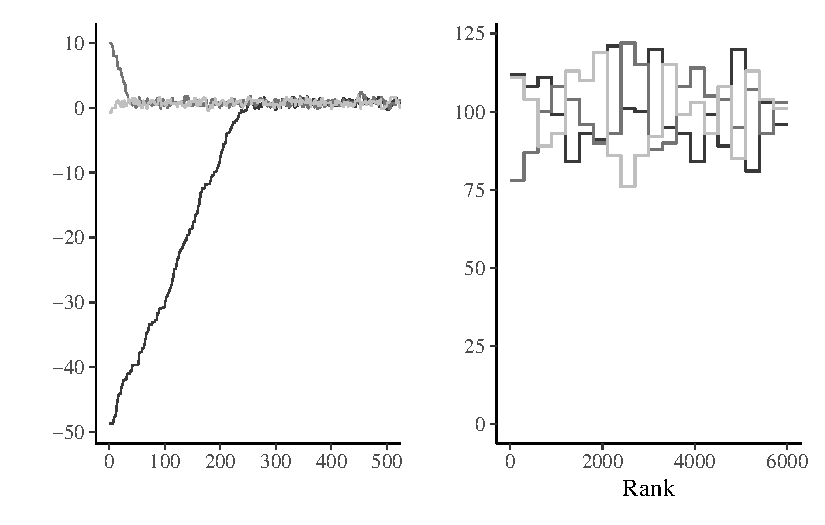
\includegraphics[keepaspectratio]{workflow_files/figure-pdf/fig-badstart-1.pdf}}

}

\caption{\label{fig-badstart}Traceplots of three Markov chains for the
same target with different initial values for the first 500 iterations
(left) and trace rank plot after discarding these (right).}

\end{figure}%

\begin{definition}[Burn in
period]\protect\hypertarget{def-burnin}{}\label{def-burnin}

We term ``burn in'' the initial steps of the MCMC algorithm that are
discarded because the chain has not reached it's stationary
distribution, due to poor starting values. , but visual inspection using
a trace plot may show that it is necessary to remove additional
observations.

\end{definition}

Most software will remove the first \(N\) initial values (typically one
thousand). Good starting values can reduce the need for a long burn in
period. If visual inspection of the chains reveal that some of the
chains for one or more parameters are not stationary until some
iteration, we will discard all of these in addition. Geweke
(\citeproc{ref-Geweke:1992}{1992})'s test measure whether the
distribution of the resulting Markov chain is the same at the beginning
and at the end through a test of equality of means.

\begin{definition}[Warmup]\protect\hypertarget{def-warmup}{}\label{def-warmup}

Warmup period refers to the initial sampling phase (potentially
overlapping with burn in period) during which proposals are tuned (for
example, by changing the variance proposal to ensure good acceptance
rate or for Hamiltonian Monte Carlo (HMC) to tune the size of the
leapfrog. These initial steps should be disregarded.

\end{definition}

The target of inference is a functional (i.e., one-dimensional summaries
of the chain): we need to have convergence of the latter, but also
sufficient effective sample size for our averages to be accurate (at
least to two significant digits).

To illustrate these, we revisit the model from
Example~\ref{exm-randomeffects} with a penalized complexity prior for
the individual effect \(\alpha_i\) and vague normal priors. We also fit
a simple Poisson model with only the fixed effect, taking
\(Y_{ij} \sim \mathsf{Poisson}\{\exp(\beta_j)\}\) with
\(\beta_j \sim \mathsf{Gauss}(0,100)\). This model has too little
variability relative to the observations and fits poorly as is.

For the Poisson example, the effective sample size for the
\(\boldsymbol{\beta}\) for the multilevel model is a bit higher than
1000 with \(B=5000\) iterations, whereas we have for the simple naive
model is \(\ensuremath{1.028\times 10^{4}}\) for \(B=10000\) draws,
suggesting superefficient sampling. The dependency between
\(\boldsymbol{\alpha}\) and \(\boldsymbol{\beta}\) is responsible for
the drop in accuracy.

The \texttt{coda} (convergence diagnosis and output analysis) \textbf{R}
package (\citeproc{ref-coda}{Plummer et al. 2006}) contains many tests.
For example, the Geweke \(Z\)-score compares the averages for the
beginning and the end of the chain: rejection of the null implies lack
of convergence, or poor mixing.

Running multiple Markov chains can be useful for diagnostics.

\begin{proposition}[Gelman--Rubin
diagnostic]\protect\hypertarget{prp-rhat}{}\label{prp-rhat}

The Gelman--Rubin diagnostic \(\widehat{R},\) introduced in Gelman and
Rubin (\citeproc{ref-Gelman.Rubin:1992}{1992}) and also called potential
scale reduction statistic, is obtained by considering the difference
between within-chains and between-chains variance. Suppose we run \(M\)
chains for \(B\) iterations, post burn in. Denoting by \(\theta_{bm}\)
the \(b\)th draw of the \(m\)th chain, we compute the global average
\(\overline{\theta} = B^{-1}M^{-1}\sum_{b=1}^B \sum_{m=1}^m \theta_{bm}\)
and similarly the chain sample average and variances, respectively
\(\overline{\theta}_m\) and \(\widehat{\sigma}^2_m\)
(\(m=1, \ldots, M\)). The between-chain variance and within-chain
variance estimator are \begin{align*}
\mathsf{Va}_{\text{between}} &= \frac{B}{M-1}\sum_{m=1}^M (\overline{\theta}_m - \overline{\theta})^2\\
\mathsf{Va}_{\text{within}} &= \frac{1}{M}\sum_{m=1}^M \widehat{\sigma}^2_m
\end{align*} and we can compute \begin{align*}
\widehat{R} = \left(\frac{\mathsf{Va}_{\text{within}}(B-1) + \mathsf{Va}_{\text{between}}}{B\mathsf{Va}_{\text{within}}}\right)^{1/2}
\end{align*} The potential scale reduction statistic must be, by
construction, larger than 1 in large sample. Any value larger than this
is indicative of problems of convergence. While the Gelman--Rubin
diagnostic is frequently reported, and any value larger than 1 deemed
problematic, it is not enough to have approximately \(\widehat{R}=1\) to
guarantee convergence, but large values are usually indication of
something being amiss. Figure~\ref{fig-rhat} shows two instances where
the chains are visually very far from having the same average and this
is reflected by the large values of \(\widehat{R}.\)

\end{proposition}

\begin{figure}[ht!]

\centering{

\pandocbounded{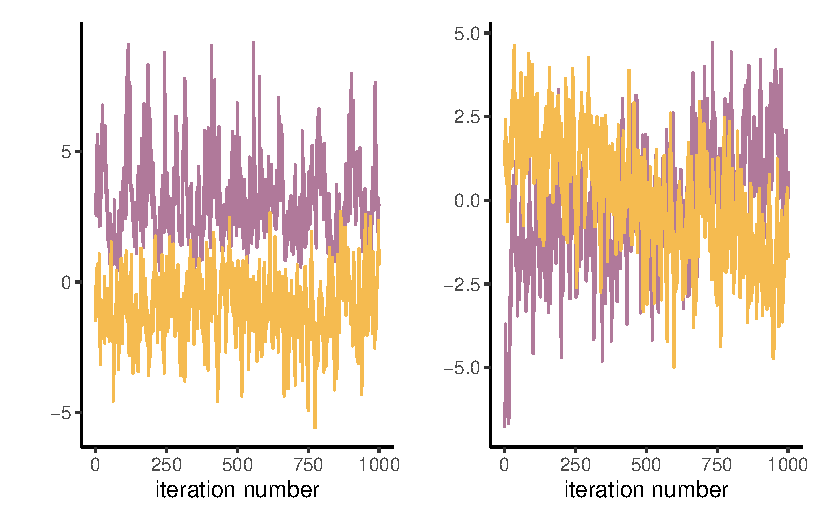
\includegraphics[keepaspectratio]{workflow_files/figure-pdf/fig-rhat-1.pdf}}

}

\caption{\label{fig-rhat}Two pairs of Markov chains: the top ones seem
stationary, but with different modes. This makes the between chain
variance substantial, with a value of \(\widehat{R} \approx 3.4,\)
whereas the chains on the right hover around the same values of zero,
but do not appear stable with \(\widehat{R} \approx 1.6.\)}

\end{figure}%

Generally, it is preferable to run a single chain for a longer period
than run multiple chains sequentially, as there is a cost to
initializing multiple times with different starting values since we must
discard initial draws. With parallel computations, multiple chains are
more frequent nowadays.

\begin{definition}[Thinning]\protect\hypertarget{def-thinning}{}\label{def-thinning}

MCMC algorithms are often run thinning the chain (i.e., keeping only a
fraction of the samples drawn, typically every \(k\) iteration). This is
wasteful as we can of course get more precise estimates by keeping all
posterior draws, whether correlated or not. The only argument in favor
of thinning is limited storage capacity: if we run very long chains in a
model with hundreds of parameters, we may run out of memory.

\end{definition}

\subsection{Posterior predictive
checks}\label{posterior-predictive-checks}

Posterior predictive checks can be used to compare models of varying
complexity.One of the visual diagnostics, outlined in Gabry et al.
(\citeproc{ref-Gabry:2019}{2019}), consists in computing a summary
statistic of interest from the posterior predictive (whether mean,
median, quantile, skewness, etc.) which is relevant for the problem at
hand and which we hope our model can adequately capture. These should be
salient features of the data, and may reveal inadequate likelihood or
prior information.

Suppose we have \(B\) draws from the posterior and simulate for each
\(n\) observations from the posterior predictive
\(p(\widetilde{\boldsymbol{y}} \mid \boldsymbol{y})\): we can benchmark
summary statistics from our original data \(\boldsymbol{y}\) with the
posterior predictive copies \(\widetilde{\boldsymbol{y}}_b.\)
Figure~\ref{fig-posterior-pred-check} shows this for the two competing
models and highlight the fact that the simpler model is not dispersed
enough. Even the more complex model struggles to capture this additional
heterogeneity with the additional variables. One could go back to the
drawing board and consider a negative binomial model.

\begin{figure}[ht!]

\centering{

\pandocbounded{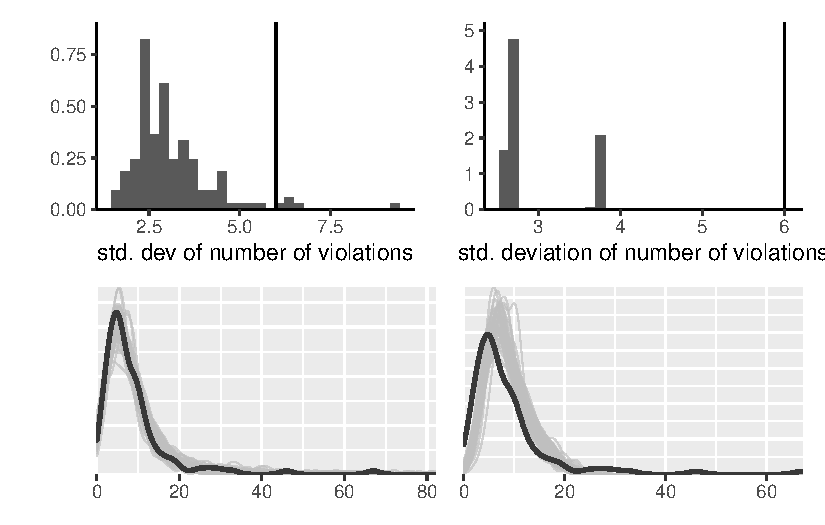
\includegraphics[keepaspectratio]{workflow_files/figure-pdf/fig-posterior-pred-check-1.pdf}}

}

\caption{\label{fig-posterior-pred-check}Posterior predictive checks for
the standard deviation (top) and density of posterior draws (bottom) for
hierarchical Poisson model with individual effects (left) and simpler
model with only conditions (right).}

\end{figure}%

\section{Information criteria}\label{information-criteria}

The widely applicable information criterion
(\citeproc{ref-Watanabe:2010}{Watanabe 2010}) is a measure of predictive
performance that approximates the cross-validation loss. Consider first
the log pointwise predictive density, defined as the expected value over
the posterior distribution
\(p(\boldsymbol{\theta} \mid \boldsymbol{y}),\) \begin{align*}
\mathsf{LPPD}_i = \mathsf{E}_{\boldsymbol{\theta} \mid \boldsymbol{y}} \left\{ \log p(y_i \mid \boldsymbol{\theta})\right\}.
\end{align*} The higher the value of the predictive density
\(\mathsf{LPPD}_i,\) the better the fit for that observation.

As in general information criteria, we sum over all observations, adding
a penalization factor that approximates the effective number of
parameters in the model, with \begin{align*}
n\mathsf{WAIC} = -\sum_{i=1}^n \mathsf{LPPD}_i + \sum_{i=1}^n \mathsf{Va}_{\boldsymbol{\theta} \mid \boldsymbol{y}}\{\log p(y_i \mid \boldsymbol{\theta})\}
\end{align*} where we use again the empirical variance to compute the
rightmost term. When comparing competing models, we can rely on their
values of \(\mathsf{WAIC}\) to discriminate about the predictive
performance. To compute \(\mathsf{WAIC},\) we need to store the values
of the log density of each observation, or at least minimally
\href{https://www.johndcook.com/blog/standard_deviation/}{compute the
running mean and variance accurately} pointwise at storage cost
\(\mathrm{O}(n).\) Note that Section 7.2 of Gelman et al.
(\citeproc{ref-Gelman:2013}{2013}) define the widely applicable
information criterion as \(2n \times \mathsf{WAIC}\) to make on par with
other information criteria, which are defined typically on the deviance
scale and so that lower values correspond to higher predictive
performance.

An older criterion which has somewhat fallen out of fashion is the
\textbf{deviance} information criterion of Spiegelhalter et al.
(\citeproc{ref-Spiegelhalter:2002}{2002}). It is defined as
\begin{align*}
\mathsf{DIC} = -2 \ell(\widetilde{\boldsymbol{\theta}}) + 2 p_D
\end{align*} where \(p_D\) is the posterior expectation of the deviance
relative to the point estimator of the parameter
\(\widetilde{\boldsymbol{\theta}}\) (e.g., the maximum a posteriori or
the posterior mean) \begin{align*}
p_D = \mathsf{E}\{D(\boldsymbol{\theta}, \widetilde{\boldsymbol{\theta}}) \mid \boldsymbol{y}\}= \int 2 \{ \ell(\widetilde{\boldsymbol{\theta}}) - \ell(\boldsymbol{\theta})\} f(\boldsymbol{\theta} \mid \boldsymbol{y}) \mathrm{d} \boldsymbol{\theta}
\end{align*} The DIC can be easily evaluated by keeping track of the log
likelihood evaluated at each posterior draw from a Markov chain Monte
Carlo algorithm. The penalty term \(p_D\) is however not invariant to
reparametrizations. Assuming we can derive a multivariate Gaussian
approximation to the MLE under suitable regularity conditions, the
\(\mathsf{DIC}\) is equivalent in large samples to \(\mathsf{AIC}.\) The
\(\mathsf{DIC}\) is considered by many authors as not being a Bayesian
procedure; see Spiegelhalter et al.
(\citeproc{ref-Spiegelhalter:2014}{2014}) and the discussion therein.

Criteria such as \(\mathsf{LPPD}\) and therefore \(\mathsf{WAIC}\)
require some form of exchangeability, and don't apply to cases where
leave-one-out cross validation isn't adequate, for example in
spatio-temporal models.

\begin{example}[Information criteria for smartwatch and Bayesian
LASSO]\protect\hypertarget{exm-smartwatch-infocriteria}{}\label{exm-smartwatch-infocriteria}

For the smartwatch model, we get a value of 3.07 for the complex model
and 4.5: this suggests an improvement in using individual-specific
effects.

\begin{Shaded}
\begin{Highlighting}[]
\CommentTok{\#\textquotesingle{} WAIC}
\CommentTok{\#\textquotesingle{} @param loglik\_pt B by n matrix of pointwise log likelihood}
\NormalTok{WAIC }\OtherTok{\textless{}{-}} \ControlFlowTok{function}\NormalTok{(loglik\_pt)\{}
  \SpecialCharTok{{-}}\FunctionTok{mean}\NormalTok{(}\FunctionTok{apply}\NormalTok{(loglik\_pt, }\DecValTok{2}\NormalTok{, mean)) }\SpecialCharTok{+}  \FunctionTok{mean}\NormalTok{(}\FunctionTok{apply}\NormalTok{(loglik\_pt, }\DecValTok{2}\NormalTok{, var))}
\NormalTok{\}}
\end{Highlighting}
\end{Shaded}

We can also look at the predictive performance. For the
\texttt{diabetes} data application with the Bayesian LASSO with fixed
\(\lambda,\) the predictive performance is a trade-off between the
effective number of parameter (with larger penalties translating into
smaller number of parameters) and the goodness-of-fit.
Figure~\ref{fig-waic-blasso} shows that the decrease in predictive
performance is severe when estimates are shrunk towards 0, but the model
performs equally well for small penalties.

\begin{figure}[ht!]

\centering{

\pandocbounded{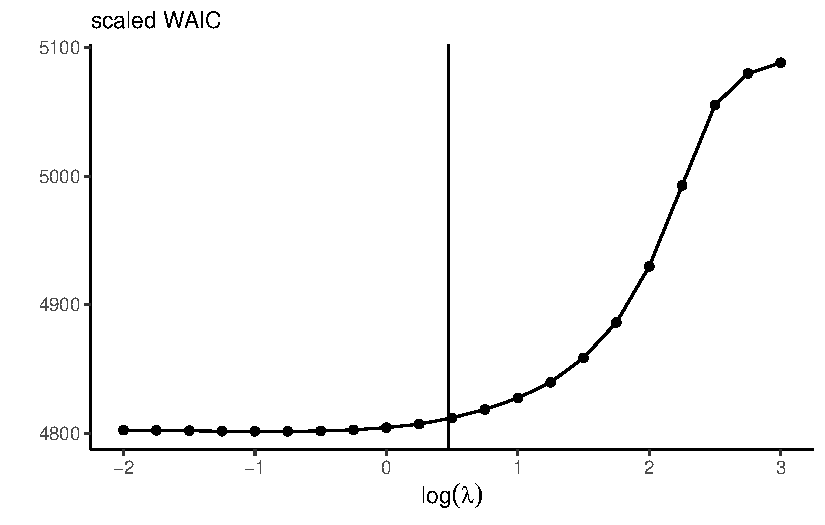
\includegraphics[keepaspectratio]{workflow_files/figure-pdf/fig-waic-blasso-1.pdf}}

}

\caption{\label{fig-waic-blasso}Widely applicable information criterion
for the Bayesian LASSO problem fitted to the diabetes data, as a
function of the penalty \(\lambda.\)}

\end{figure}%

\end{example}

Ideally, one would measure the predictive performance using the
leave-one-out predictive distribution for observation \(i\) given all
the rest, \(p(y_i \mid \boldsymbol{y}_{-i}),\) to avoid double dipping
--- the latter is computationally intractable because it would require
running \(n\) Markov chains with \(n-1\) observations each, but we can
get a good approximation using importance sampling. The \texttt{loo}
package uses this with generalized Pareto smoothing to avoid overly
large weights.

Once we have the collection of estimated
\(p(y_i \mid \boldsymbol{y}_{-i}),\) we can assess the probability level
of each observation. This gives us a set of values which should be
approximately uniform if the model was perfectly calibrated. The
probability of seeing an outcome as extreme as \(y_i\) can be obtained
by simulating draws from the posterior predictive given
\(\boldsymbol{y}_{-i}\) and computing the scaled rank of the original
observation. Values close to zero or one may indicate outliers.

\begin{figure}[ht!]

\centering{

\pandocbounded{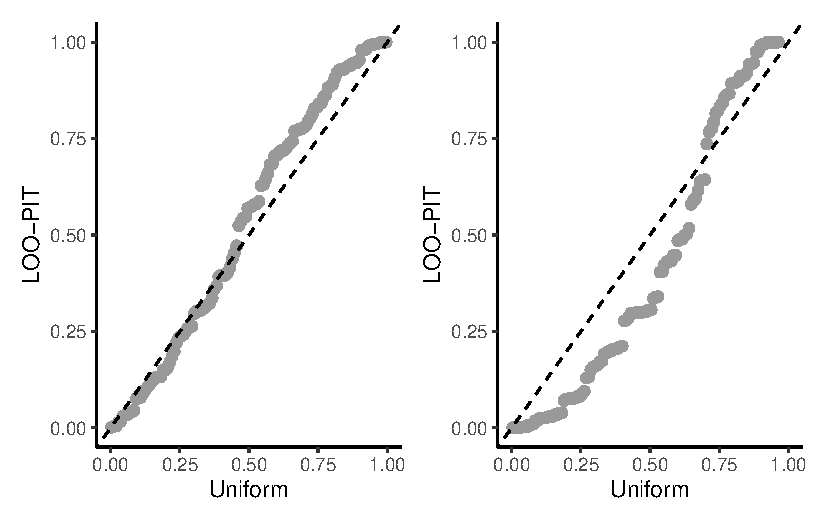
\includegraphics[keepaspectratio]{workflow_files/figure-pdf/fig-loocv-qqplots-1.pdf}}

}

\caption{\label{fig-loocv-qqplots}Quantile-quantile plots based on
leave-one-out cross validation for model for the Poisson hierarchical
model with the individual random effects (left) and without (right).}

\end{figure}%

\section{Computational strategies}\label{computational-strategies}

The data augmentation strategies considered in
Section~\ref{sec-gibbs-da} helps to simplify the likelihood and thereby
reduce the cost of each iteration. However, latent variables are imputed
conditional on current parameter values \(\boldsymbol{\theta}_a\): the
higher the number of variables, the more the model will concentrate
around current values of \(\boldsymbol{\theta}_a\), which leads to slow
mixing.

There are two main strategies to deal with this problem: blocking the
random effects together and simulating them jointly to improve mixing,
and marginalizing out over some of the latent variables.

\begin{example}[Marginalization in Gaussian
models]\protect\hypertarget{exm-marginalization-Gauss}{}\label{exm-marginalization-Gauss}

To illustrate this fact, consider a hierarchical Gaussian model of the
form \begin{align*}
\boldsymbol{Y} = \mathbf{X}\boldsymbol{\beta} + \mathbf{Z}\boldsymbol{B} + \boldsymbol{\varepsilon}
\end{align*} where \(\mathbf{X}\) is an \(n \times p\) design matrix
with centered inputs,
\(\boldsymbol{\beta} \sim \mathsf{Gauss}(\boldsymbol{0}_p, \sigma^2\mathbf{I}_p),\)
\(\boldsymbol{B}\sim \mathsf{Gauss}_q(\boldsymbol{0}_q, \boldsymbol{\Omega})\)
are random effects and
\(\boldsymbol{\varepsilon} \sim \mathsf{Gauss}_n(\boldsymbol{0}_n, \kappa^2\mathbf{I}_n)\)
are independent white noise.

We can write \begin{align*}
\boldsymbol{Y} \mid \mathbf{\beta}, \boldsymbol{B} &\sim \mathsf{Gauss}_n(\mathbf{X}\boldsymbol{\beta} + \mathbf{Z}\boldsymbol{B},  \sigma^2\mathbf{I}_p)\\
\boldsymbol{Y} \mid \mathbf{\beta} &\sim \mathsf{Gauss}_n(\mathbf{X}\boldsymbol{\beta}, \mathbf{Q}^{-1}),
\end{align*} where the second line corresponds to marginalizing out the
random effects \(\boldsymbol{B}.\) This reduces the number of parameters
to draw, but the likelihood evaluation is more costly due to
\(\mathbf{Q}^{-1}\). If, as is often the case,
\(\boldsymbol{\Omega}^{-1}\) and \(\mathbf{Z}\) are sparse matrices, the
full precision matrix can be efficiently computed using
Shermann--Morisson--Woodbury identity as \begin{align*}
\mathbf{Q}^{-1} &=   \mathbf{Z}\boldsymbol{\Omega}^{-1}\mathbf{Z}^\top + \kappa^2 \mathbf{I}_n,\\
\kappa^2\mathbf{Q} & = \mathbf{I}_n - \mathbf{Z} \boldsymbol{G}^{-1} \mathbf{Z}^\top,\\
\boldsymbol{G} &= \mathbf{Z}^\top\mathbf{Z} + \kappa^2 \boldsymbol{\Omega}^{-1}
\end{align*} Section 3.1 of Nychka et al.
(\citeproc{ref-Nychka:2015}{2015}) details efficient ways of calculating
the quadratic form involving \(\mathbf{Q}\) and it's determinant.

\end{example}

\begin{proposition}[Pseudo
marginal]\protect\hypertarget{prp-pseudo-marginal}{}\label{prp-pseudo-marginal}

Another option proposed by Andrieu and Roberts
(\citeproc{ref-Andrieu.Roberts:2009}{2009}) based on an original idea
from Beaumont (\citeproc{ref-Beaumont:2003}{2003}) relies on pseudo
marginalization, where integration is done via Monte Carlo sampling.
Specifically, suppose that we are ultimately interested in
\[p(\boldsymbol{\theta})= \int p(\boldsymbol{\theta}, \boldsymbol{z}) \mathrm{d} \boldsymbol{z},\]
but that for this purpose we normally sample from both parameters. Given
a proposal \(\boldsymbol{\theta}\) and \(q_1(\boldsymbol{\theta})\) and
subsequently \(L\) draws once from
\(q_2(\boldsymbol{z} \mid \boldsymbol{\theta})\) for the nuisance, we
can approximate the marginal using, e.g., importance sampling as
\begin{align*}
\widehat{p}(\boldsymbol{\theta}; \boldsymbol{z}) = \frac{1}{L} \sum_{l=1}^L \frac{p(\boldsymbol{\theta}, \boldsymbol{z}_l)}{q_2(\boldsymbol{z}_l, \boldsymbol{\theta})}.
\end{align*} We then run a Markov chain on an augmented state space
\(\boldsymbol{\Theta} \times \mathcal{Z}^L\), with Metropolis--Hastings
acceptance ratio of \begin{align*}
\frac{\widehat{p}(\boldsymbol{\theta}^{\star}; \boldsymbol{z}_{1,t}^{\star}, \boldsymbol{z}_{L,t}^{\star})}{
\widehat{p}(\boldsymbol{\theta}_t; \boldsymbol{z}_{1,t-1}, \ldots, \boldsymbol{z}_{L, t-1})}\frac{q_1(\boldsymbol{\theta}_{t-1} \mid \boldsymbol{\theta}^{\star}_t)}{q_1(\boldsymbol{\theta}^{\star}_t \mid \boldsymbol{\theta}_{t-1})}.
\end{align*} Note that the terms involving
\(\prod_{l=1}^L q_2(\boldsymbol{z}_{l}; \boldsymbol{\theta})\) do not
appear because they cancel out, as they are also part of the augmented
state space likelihood.

The remarkable feature of the pseudo marginal approach is that even if
our average approximation \(\widehat{p}\) to the marginal is noisy, the
marginal posterior of this Markov chain is the same as the original
target.

Compared to regular data augmentation, we must store the full vector
\(\boldsymbol{z}^{\star}_1, \ldots, \boldsymbol{z}^{\star}_L\) and
perform \(L\) evaluations of the augmented likelihood. The values of
\(\boldsymbol{z}\), if accepted, are stored for the next evaluation of
the ratio.

The idea of pseudo-marginal extends beyond the user case presented
above, as as long as we have an unbiased non-negative estimator of the
likelihood
\(\mathsf{E}\{\widehat{p}(\boldsymbol{\theta})\}=p(\boldsymbol{\theta})\),
even when the likelihood itself is intractable. This is useful for
models where we can approximate the likelihood by simulation, like for
particle filters. Pseudo marginal MCMC algorithms are notorious for
yielding sticky chains.

\end{proposition}

\begin{proposition}[Blocking]\protect\hypertarget{prp-blocking}{}\label{prp-blocking}

When parameters of the vector \(\boldsymbol{\theta}\) that we wish to
sample are strongly correlated, it is advisable when possible to
simulate them jointly. Because the unnormalized posterior is evaluated
at each step conditional on all values, the Markov chain will be making
incremental moves and mix slowly if we sample them one step at a time.

\end{proposition}

Before showcasing the effect of blocking and joint updates, we present
another example of data augmentation using
Example~\ref{exm-probit-regression}.

\begin{example}[Tokyo
rainfall]\protect\hypertarget{exm-Tokyo-rainfall}{}\label{exm-Tokyo-rainfall}

We consider data from Kitagawa (\citeproc{ref-Kitagawa:1987}{1987}) that
provide a binomial time series giving the number of days in years 1983
and 1984 (a leap year) in which there was more than 1mm of rain in
Tokyo. These data and the model we consider are discussed in in section
4.3.4 of H. Rue and Held (\citeproc{ref-Rue.Held:2005}{2005}). We thus
have \(T=366\) days and \(n_t \in \{1,2\}\) \((t=1, \ldots, T)\) the
number of observations in day \(t\) and \(y_t=\{0,\ldots, n_t\}\) the
number of days with rain. The objective is to obtain a smoothed
probability of rain. The underlying probit model considered takes
\(Y_t \mid n_t, p_t \sim \mathsf{binom}(n_t, p_t)\) and
\(p_t = \Phi(\beta_t).\)

We specify the random effects
\(\boldsymbol{\beta} \sim \mathsf{Gauss}_{T}(\boldsymbol{0}, \tau^{-1}\mathbf{Q}^{-1}),\)
where \(\mathbf{Q}\) is a \(T \times T\) precision matrix that encodes
the local dependence. A circular random walk structure of order 2 is
used to model the smooth curves by smoothing over neighbors, and
enforces small second derivative. This is a suitable prior because it
enforces no constraint on the mean structure. This amounts to specifying
the process with \begin{align*}
\Delta^2\beta_t &= (\beta_{t+1} - \beta_t) - (\beta_t - \beta_{t-1})
\\&=-\beta_{t-1} +2 \beta_t - \beta_{t+1} \sim \mathsf{Gauss}(0, \tau^{-1}), \qquad t \in \mathbb{N} \mod 366.
\end{align*} This yields an intrinsic Gaussian Markov random field with
a circulant precision matrix \(\tau\mathbf{Q}=\tau\mathbf{GG^\top}\) of
rank \(T-1,\) where \begin{align*}
\mathbf{G} &=
\begin{pmatrix}
2 & -1 & 0 & 0 & \cdots & -1\\
-1 & 2 & -1 & 0 & \ddots & 0 \\
0 & -1 & 2 & -1 & \ddots & 0 \\
\vdots & \ddots & \ddots  & \ddots  & \ddots  & \vdots \\
-1 & 0 & 0 & 0 & \cdots & 2
\end{pmatrix},
\\
\mathbf{Q} &=
\begin{pmatrix}
6 & -4 & 1 & 0 & \cdots & 1 & -4\\
-4 & 6 & -4 & 1 & \ddots & 0 & 1 \\
1 & -4 & 6 & -4 & \ddots & 0 & 0 \\
\vdots & \ddots & \ddots  & \ddots  & \ddots  & \ddots & \vdots \\
-4 & 1 & 0 & 0 & \cdots & -4 & 6
\end{pmatrix}.
\end{align*} Because of the linear dependency, the determinant of
\(\mathbf{Q}\) is zero. The contribution from the latent mean parameters
is multivariate Gaussian and we exploit for computations the sparsity of
the precision matrix \(\mathbf{Q}.\) Figure~\ref{fig-CRW2-prior} shows
five draws from the prior model, which loops back between December 31st
and January 1st, and is rather smooth.

\begin{figure}[ht!]

\centering{

\pandocbounded{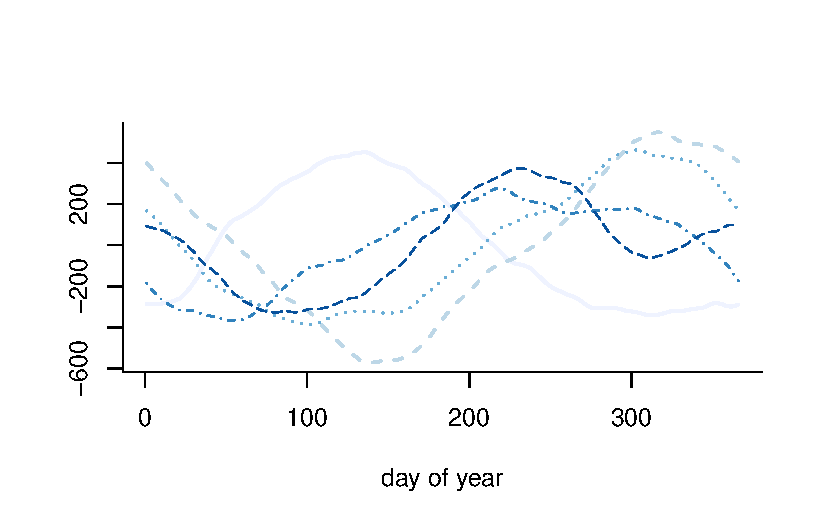
\includegraphics[keepaspectratio]{workflow_files/figure-pdf/fig-CRW2-prior-1.pdf}}

}

\caption{\label{fig-CRW2-prior}Five realizations from the cyclical
random walk Gaussian prior of order 2.}

\end{figure}%

We can perform data augmentation by imputing Gaussian variables, say
\(\{z_{t,i}\}\) following Example~\ref{exm-probit-regression} from
truncated Gaussian, where \(z_{t,i} = \beta_t + \varepsilon_{t,i}\) and
\(\varepsilon_{t,i} \sim \mathsf{Gauss}(0,1)\) are independent standard
Gaussian and \begin{align*}
z_{t,i} \mid  y_{t,i}, \beta_t \sim 
\begin{cases}
\mathsf{trunc. Gauss}(\beta_t, 1, -\infty, 0) & y_{t,i} = 0 \\
\mathsf{trunc. Gauss}(\beta_t, 1,  0, \infty) & y_{t,i} =1 
\end{cases}
\end{align*} The posterior is proportional to \begin{align*}
p(\boldsymbol{\beta} \mid \tau)p(\tau)\prod_{t=1}^{T}\prod_{i=1}^{n_t}p(y_{t,i} \mid z_{t,i}) p(z_{t,i} \mid \beta_t)
\end{align*} and once we have imputed the Gaussian latent vectors, we
can work directly with the values of \(z_t = \sum_{i=1}^{n_t} z_{i,t}.\)
The posterior then becomes \begin{align*}
p(\boldsymbol{\beta}, \tau) &\propto \tau^{(n-1)/2}\exp \left( - \frac{\tau}{2} \boldsymbol{\beta}^\top \mathbf{Q} \boldsymbol{\beta}\right)\tau^{a-1}\exp(-\tau b)\\& \quad \times \exp\left\{ - \frac{1}{2} (\boldsymbol{z}/\boldsymbol{n} - \boldsymbol{\beta})^\top \mathrm{diag}(\boldsymbol{n})(\boldsymbol{z}/\boldsymbol{n} - \boldsymbol{\beta})\right\} 
\end{align*} where \(\boldsymbol{z} = (z_1, \ldots, z_T).\) Completing
the quadratic form shows that \begin{align*}
\boldsymbol{\beta} \mid \boldsymbol{z}, \tau &\sim \mathsf{Gauss}_T\left[\left\{\tau \mathbf{Q} + \mathrm{diag}(\boldsymbol{n})\right\}^{-1} \boldsymbol{z}, \left\{\tau \mathbf{Q} + \mathrm{diag}(\boldsymbol{n})\right\}^{-1}\right]\\
\tau \mid \boldsymbol{\beta} & \sim \mathsf{gamma}\left( \frac{n-1}{2} + a, \frac{\boldsymbol{\beta}^\top \mathbf{Q}\boldsymbol{\beta}}{2} + b \right)
\end{align*}

\begin{Shaded}
\begin{Highlighting}[]
\FunctionTok{library}\NormalTok{(Matrix)}
\FunctionTok{library}\NormalTok{(TruncatedNormal)}
\FunctionTok{data}\NormalTok{(tokyorain, }\AttributeTok{package =} \StringTok{"hecbayes"}\NormalTok{)}
\CommentTok{\# Aggregate data}
\NormalTok{tokyo }\OtherTok{\textless{}{-}}\NormalTok{ tokyorain }\SpecialCharTok{|\textgreater{}} 
\NormalTok{   dplyr}\SpecialCharTok{::}\FunctionTok{group\_by}\NormalTok{(day) }\SpecialCharTok{|\textgreater{}}
\NormalTok{   dplyr}\SpecialCharTok{::}\FunctionTok{summarize}\NormalTok{(}\AttributeTok{y =} \FunctionTok{sum}\NormalTok{(y), }\AttributeTok{n =}\NormalTok{ dplyr}\SpecialCharTok{::}\FunctionTok{n}\NormalTok{())}
\NormalTok{nt }\OtherTok{\textless{}{-}} \DecValTok{366}\NormalTok{L}
\CommentTok{\# Circulant random walk of order two precision matrix}
\NormalTok{Q }\OtherTok{\textless{}{-}}\NormalTok{ hecbayes}\SpecialCharTok{::}\FunctionTok{crw\_Q}\NormalTok{(}\AttributeTok{d =}\NormalTok{ nt, }\AttributeTok{type =} \StringTok{"rw2"}\NormalTok{, }\AttributeTok{sparse =} \ConstantTok{TRUE}\NormalTok{)}
\CommentTok{\# Sparse Cholesky root}
\NormalTok{cholQ }\OtherTok{\textless{}{-}}\NormalTok{ Matrix}\SpecialCharTok{::}\FunctionTok{chol}\NormalTok{(Q)}
\NormalTok{N }\OtherTok{\textless{}{-}}\NormalTok{ Matrix}\SpecialCharTok{::}\FunctionTok{Diagonal}\NormalTok{(}\AttributeTok{n =}\NormalTok{ nt, }\AttributeTok{x =}\NormalTok{ tokyo}\SpecialCharTok{$}\NormalTok{n)}
\CommentTok{\# Create containers}
\NormalTok{B }\OtherTok{\textless{}{-}} \FloatTok{1e4}\NormalTok{L }\CommentTok{\# number of draws}
\NormalTok{beta\_s }\OtherTok{\textless{}{-}} \FunctionTok{matrix}\NormalTok{(}\AttributeTok{nrow =}\NormalTok{ B, }\AttributeTok{ncol =}\NormalTok{ nt)}
\NormalTok{x\_s }\OtherTok{\textless{}{-}} \FunctionTok{matrix}\NormalTok{(}\AttributeTok{nrow =}\NormalTok{ B, }\AttributeTok{ncol =}\NormalTok{ nt)}
\NormalTok{tau\_s }\OtherTok{\textless{}{-}} \FunctionTok{numeric}\NormalTok{(B)}
\CommentTok{\# Initial values}
\NormalTok{beta }\OtherTok{\textless{}{-}} \FunctionTok{rep}\NormalTok{(}\DecValTok{0}\NormalTok{, nt)}
\NormalTok{tau }\OtherTok{\textless{}{-}} \DecValTok{1000}
\CommentTok{\# Hyperprior parameter values}
\NormalTok{tau\_a }\OtherTok{\textless{}{-}} \DecValTok{1}
\NormalTok{tau\_b }\OtherTok{\textless{}{-}} \FloatTok{0.0001}
\CommentTok{\# Gibbs sampling}
\ControlFlowTok{for}\NormalTok{(b }\ControlFlowTok{in} \FunctionTok{seq\_len}\NormalTok{(B))\{}
  \CommentTok{\# Step 1: data augmentation}
\NormalTok{  x }\OtherTok{\textless{}{-}}\NormalTok{ TruncatedNormal}\SpecialCharTok{::}\FunctionTok{rtnorm}\NormalTok{(}
    \AttributeTok{n =} \DecValTok{1}\NormalTok{,  }\AttributeTok{mu =}\NormalTok{ beta[tokyorain}\SpecialCharTok{$}\NormalTok{day], }\AttributeTok{sd =} \DecValTok{1}\NormalTok{,}
    \AttributeTok{lb =} \FunctionTok{ifelse}\NormalTok{(tokyorain}\SpecialCharTok{$}\NormalTok{y }\SpecialCharTok{==} \DecValTok{0}\NormalTok{, }\SpecialCharTok{{-}}\ConstantTok{Inf}\NormalTok{, }\DecValTok{0}\NormalTok{),}
    \AttributeTok{ub =} \FunctionTok{ifelse}\NormalTok{(tokyorain}\SpecialCharTok{$}\NormalTok{y }\SpecialCharTok{==} \DecValTok{0}\NormalTok{, }\DecValTok{0}\NormalTok{, }\ConstantTok{Inf}\NormalTok{))}
\NormalTok{  tx }\OtherTok{\textless{}{-}} \FunctionTok{aggregate}\NormalTok{(}\AttributeTok{x =}\NormalTok{ x, }\AttributeTok{by =} \FunctionTok{list}\NormalTok{(tokyorain}\SpecialCharTok{$}\NormalTok{day), }\AttributeTok{FUN =}\NormalTok{ sum)}\SpecialCharTok{$}\NormalTok{x}
\NormalTok{  x\_s[b,] }\OtherTok{\textless{}{-}}\NormalTok{ tx}
  \CommentTok{\# Step 2: Simulate random effects in block}
\NormalTok{  beta }\OtherTok{\textless{}{-}}\NormalTok{ beta\_s[b,] }\OtherTok{\textless{}{-}} \FunctionTok{c}\NormalTok{(hecbayes}\SpecialCharTok{::}\FunctionTok{rGaussQ}\NormalTok{(}
    \AttributeTok{n =} \DecValTok{1}\NormalTok{,}
    \AttributeTok{b =}\NormalTok{ tx, }
    \AttributeTok{Q =}\NormalTok{ tau }\SpecialCharTok{*}\NormalTok{ Q }\SpecialCharTok{+}\NormalTok{ N))}
\CommentTok{\# Simulate precision}
\NormalTok{  tau }\OtherTok{\textless{}{-}}\NormalTok{ tau\_s[b] }\OtherTok{\textless{}{-}} \FunctionTok{rgamma}\NormalTok{(}
    \AttributeTok{n =} \DecValTok{1}\NormalTok{, }
    \AttributeTok{shape =}\NormalTok{ (nt}\DecValTok{{-}1}\NormalTok{)}\SpecialCharTok{/}\DecValTok{2} \SpecialCharTok{+}\NormalTok{ tau\_a, }
    \AttributeTok{rate =} \FloatTok{0.5}\SpecialCharTok{*}\FunctionTok{as.numeric}\NormalTok{(}\FunctionTok{crossprod}\NormalTok{(cholQ }\SpecialCharTok{\%*\%}\NormalTok{ beta)) }\SpecialCharTok{+}\NormalTok{ tau\_b)}
  \CommentTok{\# if beta is VERY smooth, then precision is large}
\NormalTok{\}}
\end{Highlighting}
\end{Shaded}

\begin{figure}[ht!]

\centering{

\pandocbounded{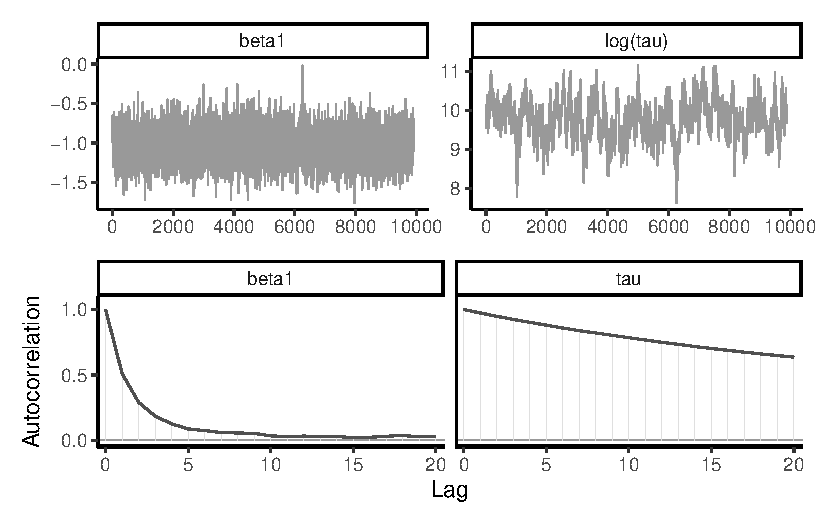
\includegraphics[keepaspectratio]{workflow_files/figure-pdf/fig-tokyo-post1-1.pdf}}

}

\caption{\label{fig-tokyo-post1}Trace plots (top) and correlograms
(bottom) for two parameters of the Gibbs sampler for the Tokyo rainfall
data, with block updates.}

\end{figure}%

\begin{figure}[ht!]

\centering{

\pandocbounded{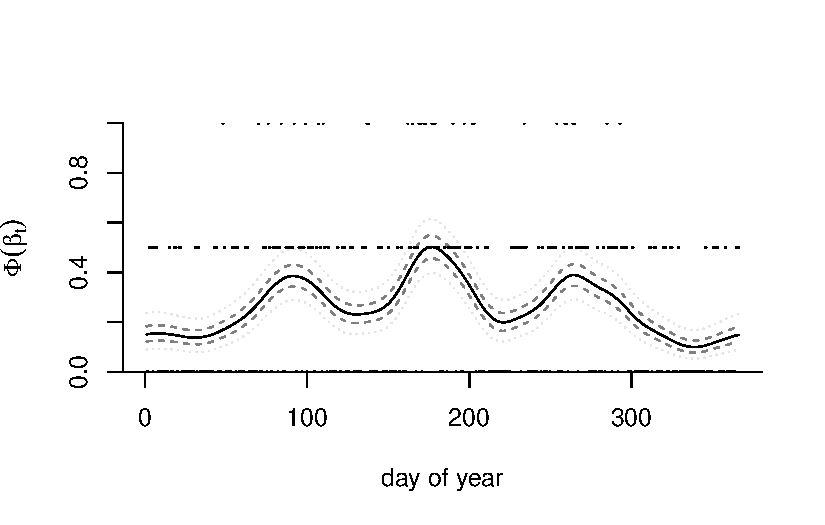
\includegraphics[keepaspectratio]{workflow_files/figure-pdf/fig-rainfall-1.pdf}}

}

\caption{\label{fig-rainfall}Tokyo rainfall fitted median probability
with 50\% and 89\% pointwise credible intervals as a function of time of
the year, with the proportion of days of rain (points).}

\end{figure}%

\end{example}

\begin{example}[Blocking]\protect\hypertarget{exm-blocking-rainfall}{}\label{exm-blocking-rainfall}

We revisit Example~\ref{exm-Tokyo-rainfall} with two modifications:
imputing one parameter \(\beta_t\) at a time using random scan Gibbs
step, which leads to slower mixing but univariate updates, and a joint
update that first draws \(\tau^{\star}\) from some proposal
distribution, then sample conditional on that value generates the
\(\boldsymbol{\beta}\) vector and proposes acceptance using a Metropolis
step.

A different (less efficient) strategy would be to simulate the
\(\beta_t\) terms one at a time using a random scan Gibbs, i.e., picking
\(t_0 \in \{1, \ldots, 366\}\) and looping over indices. This yields
higher autocorrelation between components than sampling by block.

\begin{Shaded}
\begin{Highlighting}[]
  \CommentTok{\# Compute mean vector for betas}
\NormalTok{  mbeta }\OtherTok{\textless{}{-}}\NormalTok{ Matrix}\SpecialCharTok{::}\FunctionTok{solve}\NormalTok{(}\AttributeTok{a =}\NormalTok{ tau}\SpecialCharTok{*}\NormalTok{Q }\SpecialCharTok{+}\NormalTok{ N, }\AttributeTok{b =}\NormalTok{ tx)}
  \CommentTok{\# weights of precision for neighbours}
\NormalTok{  nw }\OtherTok{\textless{}{-}} \FunctionTok{c}\NormalTok{(}\DecValTok{1}\NormalTok{, }\SpecialCharTok{{-}}\DecValTok{4}\NormalTok{, }\SpecialCharTok{{-}}\DecValTok{4}\NormalTok{, }\DecValTok{1}\NormalTok{)}
  \CommentTok{\# Sample an index at random}
\NormalTok{  st }\OtherTok{\textless{}{-}} \FunctionTok{sample.int}\NormalTok{(nt, }\DecValTok{1}\NormalTok{)}
  \ControlFlowTok{for}\NormalTok{(i }\ControlFlowTok{in}\NormalTok{ (st }\SpecialCharTok{+} \FunctionTok{seq\_len}\NormalTok{(nt)) }\SpecialCharTok{\%\%}\NormalTok{ nt }\SpecialCharTok{+} \DecValTok{1}\NormalTok{L)\{}
   \CommentTok{\# Indices of the non{-}zero entries for row Q[i,]}
\NormalTok{  nh }\OtherTok{\textless{}{-}} \FunctionTok{c}\NormalTok{(i}\DecValTok{{-}3}\NormalTok{, i}\DecValTok{{-}2}\NormalTok{, i, i}\SpecialCharTok{+}\DecValTok{1}\NormalTok{) }\SpecialCharTok{\%\%} \DecValTok{366} \SpecialCharTok{+} \DecValTok{1}
\NormalTok{  prec }\OtherTok{\textless{}{-}}\NormalTok{ tau }\SpecialCharTok{*} \DecValTok{6} \SpecialCharTok{+}\NormalTok{ tokyo}\SpecialCharTok{$}\NormalTok{n[i]}
\NormalTok{  condmean }\OtherTok{\textless{}{-}}\NormalTok{ mbeta[i] }\SpecialCharTok{{-}} \FunctionTok{sum}\NormalTok{(nw}\SpecialCharTok{*}\NormalTok{(beta[nh] }\SpecialCharTok{{-}}\NormalTok{ mbeta[nh])) }\SpecialCharTok{*}\NormalTok{ tau }\SpecialCharTok{/}\NormalTok{ prec}
\NormalTok{    beta[i] }\OtherTok{\textless{}{-}} \FunctionTok{rnorm}\NormalTok{(}\AttributeTok{n =} \DecValTok{1}\NormalTok{, }\AttributeTok{mean =}\NormalTok{ condmean, }\AttributeTok{sd =} \DecValTok{1}\SpecialCharTok{/}\FunctionTok{sqrt}\NormalTok{(prec))}
\NormalTok{  \}}
\NormalTok{  beta\_s[b,] }\OtherTok{\textless{}{-}}\NormalTok{ beta}
\end{Highlighting}
\end{Shaded}

\begin{figure}[ht!]

\centering{

\pandocbounded{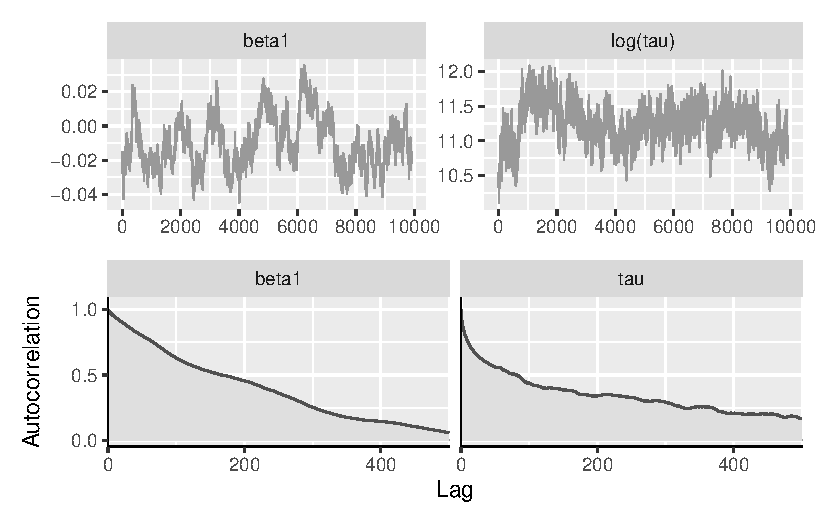
\includegraphics[keepaspectratio]{workflow_files/figure-pdf/fig-tokyo-post2-1.pdf}}

}

\caption{\label{fig-tokyo-post2}Trace plots (top) and correlograms
(bottom) for two parameters of the Gibbs sampler for the Tokyo rainfall
data, with individual updates for \(\beta_t\).}

\end{figure}%

Instead of making things worst, we can try to improve upon our initial
sampler by simulating first a proposal \(\tau^{\star}\) using a random
walk Metropolis (on the log scale) or some other proposal
\(q(\tau^{\star}; \tau),\) then drawing from the full conditional
\(\boldsymbol{\beta} \mid \boldsymbol{z}, \tau^{\star}\) and
accepting/rejecting the whole move. In doing this, all terms that depend
on \(\boldsymbol{\beta}\) cancel out, and the term
\(p(\tau^{\star}, \boldsymbol{\beta}^{\star} \mid \tau)/\{q(\tau^{\star}; \tau)p(\boldsymbol{\beta}^{\star} \mid \tau^{\star})\}\)
in the acceptance ratio becomes \begin{align*}
\frac{\tau_t^{\star(n-1)/2} p(\tau_t^{\star})\exp \left\{-\frac{1}{2}\boldsymbol{z}^\top(\boldsymbol{z}/\boldsymbol{n})\right\}}{q(\tau^{\star}; \tau) \left| \tau^{\star}\mathbf{Q} + \mathrm{diag}(\boldsymbol{n})\right|\exp \left[-\frac{1}{2}\boldsymbol{z}^\top \left\{\tau^{\star}\mathbf{Q} + \mathrm{diag}(\boldsymbol{n})\right\}^{-1}\boldsymbol{z}\right]}
\end{align*}

A second alternative is to ditch altogether the data augmentation step
and write the unnormalized log posterior for \(\boldsymbol{\beta}\) as
\begin{align*}
 \log p(\boldsymbol{\beta} \mid \boldsymbol{y}) \stackrel{\boldsymbol{\beta}}{\propto} - \frac{\tau}{2} \boldsymbol{\beta}^\top \mathbf{Q} \boldsymbol{\beta} + \sum_{t=1}^{366} y_{t} \log \Phi(\beta_t) + (n_t-y_{t}) \log\{1-\Phi(\beta_t)\}
\end{align*} and do a quadratic approximation to the posterior by doing
a Taylor expansion of the terms \(\log p(y_{t} \mid \beta_{t})\) around
the current value of the draw for \(\boldsymbol{\beta}.\) Given that
observations are conditionally independent, we have a sum of independent
terms
\(\ell(\boldsymbol{y}; \boldsymbol{\beta}) = \sum_{t=1}^{366}\log p(y_t \mid \beta_t)\)
and this yields, expanding around \(\boldsymbol{\beta}^0\), the Gaussian
Markov field proposal \begin{align*}
q(\boldsymbol{\beta} \mid \tau, \boldsymbol{\beta}^0)  \sim \mathsf{Gauss}_{366}\left[\ell'(\boldsymbol{\beta}^0), \tau\mathbf{Q} + \mathrm{diag}\{\ell''(\boldsymbol{\beta}^0)\}\right].
\end{align*} Indeed, because of conditional independence, the \(j\)th
element of \(\ell'\) and \(\ell''\) are \begin{align*}
\ell'(\boldsymbol{\beta}^0)_j  = \left. \frac{\partial \ell(y_j; \beta_j)}{\partial \beta_j}\right|_{\beta_j = \beta_j^0}, \quad \ell''(\boldsymbol{\beta}^0)_j  = \left. \frac{\partial^2 \ell(y_j; \beta_j)}{\partial \beta_j^2}\right|_{\beta_j = \beta_j^0}.
\end{align*} We can then simulate \(\tau\) using an random walk step,
then propose \(\boldsymbol{\beta}\) conditional on this value using the
Gaussian approximation above and accept/reject the pair
\((\tau, \boldsymbol{\beta})\) using a Metropolis step. As for the
Metropolis-adjusted Langevin algorithm, we need to compute the backward
move for the acceptance ratio. We refer to Section 4.4.1 of H. Rue and
Held (\citeproc{ref-Rue.Held:2005}{2005}) for more details.

\end{example}

\bookmarksetup{startatroot}

\chapter{Regression models}\label{regression-models}

This chapter is dedicated to the study of regression models from a
Bayesian standpoint. Starting with Gaussian data, we investigate the
link between frequentist approaches to regularization and shrinkage
priors. We also look at hierarchical models with mixed effects and
variable selection using reversible jump MCMC and conditional Bayes
factor.

Throughout, we consider regression models with model (or design) matrix
\(\mathbf{X} \in \mathbb{R}^{n \times p}\) with centered inputs, so
\(\mathbf{1}_n^\top\mathbf{X}=\mathbf{0}_p.\) We are interested in the
associated vector of regression coefficients
\(\boldsymbol{\beta} = (\beta_1, \ldots, \beta_p)^\top\) which describe
the mean and act as weights for each covariate vector. In the ordinary
linear regression model \begin{align*}
\boldsymbol{Y} \mid \mathbf{X}, \boldsymbol{\beta}, \omega \sim \mathsf{Gauss}_n(\beta_0\mathbf{1}_n + \mathbf{X}\boldsymbol{\beta}, \omega^{-1}\mathbf{I}_n),
\end{align*} so that observations are independent and homoscedastic.
Inference is performed conditional on the observed covariate vectors
\(\mathbf{X}_i\); we omit this dependence hereafter, but note that this
can be relaxed. The intercept \(\beta_0\), which is added to capture the
mean response and make it mean-zero, receives special treatment and is
typically assigned an improper prior. We largely follow the exposition
of Villani (\citeproc{ref-Villani:2023}{2023}).

Before we proceed with analysis of the Gaussian linear model, we derive
a useful formula for completion of quadratic forms that arise in
Gaussian models.

\begin{proposition}[Decomposition of quadratic
forms]\protect\hypertarget{prp-quadratic-forms}{}\label{prp-quadratic-forms}

For quadratic forms (in \(\boldsymbol{x}\)) with \begin{align*}
& (\boldsymbol{x} - \boldsymbol{a})^\top \mathbf{A}(\boldsymbol{x} - \boldsymbol{a}) + (\boldsymbol{x} - \boldsymbol{b})^\top \mathbf{B}(\boldsymbol{x} - \boldsymbol{b}) \\\quad &=
 (\boldsymbol{x} - \boldsymbol{c})^\top \mathbf{C}(\boldsymbol{x} - \boldsymbol{c}) + (\boldsymbol{c}-\boldsymbol{a})^\top\mathbf{A}(\boldsymbol{c}-\boldsymbol{a}) + (\boldsymbol{c}-\boldsymbol{b})^\top\mathbf{B}(\boldsymbol{c}-\boldsymbol{b})\\
&\stackrel{\boldsymbol{x}}{\propto} (\boldsymbol{x} - \boldsymbol{c})^\top \mathbf{C}(\boldsymbol{x} - \boldsymbol{c})
\end{align*} where \(\mathbf{C} = \mathbf{A} + \mathbf{B}\) and
\(\boldsymbol{c}= \mathbf{C}^{-1}(\mathbf{A}\boldsymbol{a} + \mathbf{B}\boldsymbol{b})\).

\end{proposition}

\begin{proposition}[Gaussian ordinary linear regression with conjugate
priors]\protect\hypertarget{prp-gaussian-ols}{}\label{prp-gaussian-ols}

The conjugate prior for the Gaussian regression model for the mean and
precision parameters \(\boldsymbol{\beta}\) and \(\omega\),
respectively, is a Gaussian-gamma and is defined hierarchically as
\begin{align*}
\boldsymbol{\beta} \mid \omega &\sim \mathsf{Gauss}\left\{\boldsymbol{\mu}_0, (
\omega\boldsymbol{\Omega}_0)^{-1}\right\} \\
\omega &\sim \mathsf{gamma}(\nu_0/2,\tau_0/2).
\end{align*} Using properties of the Gaussian distribution, the sampling
distribution of the ordinary least squares estimator is
\(\widehat{\boldsymbol{\beta}} \sim \mathsf{Gauss}_p\{\boldsymbol{\beta}, (\omega\mathbf{X}^\top\mathbf{X})^{-1}\}\).

The conditional and marginal posterior distributions for the mean
coefficients \(\boldsymbol{\beta}\) and for the precision \(\omega\) are
\begin{align*}
\boldsymbol{\beta} \mid \omega, \boldsymbol{y} &\sim \mathsf{Gauss}_p\left\{\boldsymbol{\mu}_n, (\omega\boldsymbol{\Omega}_n)^{-1}\right\}  \\
\omega \mid  \boldsymbol{y} &\sim \mathsf{gamma}\left\{(\nu_0 + n)/2,  \tau^2_n/2\right\}, \\
\boldsymbol{\beta} \mid  \boldsymbol{y} &\sim \mathsf{Student}_p(\boldsymbol{\mu}_n,  \tau_n/(\nu_0+n) \times \mathbf{\Omega}_n^{-1}, \nu_0 + n)
\end{align*} where \begin{align*}
\boldsymbol{\Omega}_n &= \mathbf{X}^\top\mathbf{X} + \boldsymbol{\Omega}_0\\
\boldsymbol{\mu}_n &= \boldsymbol{\Omega}_n^{-1}(\mathbf{X}^\top\mathbf{X}\widehat{\boldsymbol{\beta}} + \boldsymbol{\Omega}_0\boldsymbol{\mu}_0) = \boldsymbol{\Omega}_n^{-1}(\mathbf{X}^\top\boldsymbol{y} + \boldsymbol{\Omega}_0\boldsymbol{\mu}_0)\\
\tau_n &= \tau_0 + (\boldsymbol{y} - \mathbf{X}\widehat{\boldsymbol{\beta}})^\top(\boldsymbol{y} - \mathbf{X}\widehat{\boldsymbol{\beta}}) + (\boldsymbol{\mu}_n - \widehat{\boldsymbol{\beta}})^\top \mathbf{X}^\top\mathbf{X}(\boldsymbol{\mu}_n - \widehat{\boldsymbol{\beta}}) \\& \quad + (\boldsymbol{\mu}_n-\boldsymbol{\mu}_0)^\top\boldsymbol{\Omega}_0(\boldsymbol{\mu}_n-\boldsymbol{\mu}_0)
\end{align*}

\end{proposition}

\begin{proof}
Write the posterior as \begin{align*}
 p(\boldsymbol{\beta}, \omega \mid \boldsymbol{y}) &\propto p(\boldsymbol{y} \mid \boldsymbol{\beta}, \omega) p(\omega)
 \\& \propto  \omega^{n/2} \exp\left\{-\frac{\omega}{2}(\boldsymbol{y}-\mathbf{X}\boldsymbol{\beta})^\top(\boldsymbol{y}-\mathbf{X}\boldsymbol{\beta})\right\}\\& \times |\omega\boldsymbol{\Omega}_0|^{1/2}\exp \left\{ -\frac{\omega}{2} (\boldsymbol{\beta}-\boldsymbol{\mu}_0)^\top\boldsymbol{\Omega}_0(\boldsymbol{\beta}-\boldsymbol{\mu}_0)\right\} \\& \times \omega^{\nu_0/2-1}\exp\left(-\tau_0\omega/2\right).
\end{align*} We rewrite the first quadratic form in
\(\boldsymbol{y}-\mathbf{X}\boldsymbol{\beta}\) using the orthogonal
decomposition \begin{align*}
 (\boldsymbol{y}-\mathbf{X}\widehat{\boldsymbol{\beta}}) + (\mathbf{X}\widehat{\boldsymbol{\beta}} - \mathbf{X}\boldsymbol{\beta})
\end{align*} since
\((\boldsymbol{y}-\mathbf{X}\widehat{\boldsymbol{\beta}})^\top (\mathbf{X}\widehat{\boldsymbol{\beta}} - \mathbf{X}\boldsymbol{\beta}) = 0.\)
We can pull terms together and separate the conditional posterior
\(p(\boldsymbol{\beta} \mid \boldsymbol{y}, \omega)\) and
\(p(\omega \mid \boldsymbol{y})\) as \begin{align*}
 p(\boldsymbol{\beta}, \omega \mid \boldsymbol{y}) &\propto \omega^{(n+p+\nu_0)/2 -1} \exp\left[-\frac{\omega}{2}\left\{\tau_0 + (\boldsymbol{y}-\mathbf{X}\widehat{\boldsymbol{\beta}})^\top(\boldsymbol{y}-\mathbf{X}\widehat{\boldsymbol{\beta}})\right\}\right]
 \\& \times \exp \left[-\frac{\omega}{2}\left\{(\widehat{\boldsymbol{\beta}} - \boldsymbol{\beta})^\top\mathbf{X}^\top\mathbf{X}(\widehat{\boldsymbol{\beta}} - \boldsymbol{\beta})+ (\boldsymbol{\beta}-\boldsymbol{\mu}_0)^\top\boldsymbol{\Omega}_0(\boldsymbol{\beta}-\boldsymbol{\mu}_0)\right\}\right]
\end{align*} and using Proposition~\ref{prp-quadratic-forms} for the
terms in the exponent with
\(\boldsymbol{a} = \widehat{\boldsymbol{\beta}}\),
\(\mathbf{A}=\mathbf{X}^\top\mathbf{X}\),
\(\boldsymbol{b} = \boldsymbol{\mu}_0\) and
\(\mathbf{B}=\boldsymbol{\Omega}_0\), we find \begin{align*}
  p(\boldsymbol{\beta}, \omega \mid \boldsymbol{y}) & \propto
   \omega^{(n+\nu_0)/2 -1} \exp\left(-\frac{\omega\tau_n}{2}\right)
   \\& \times \omega^{p/2}\exp\left\{-\frac{1}{2}(\boldsymbol{\beta} - \boldsymbol{\mu}_n)^\top(\omega\mathbf{\Omega}_n)(\boldsymbol{\beta} - \boldsymbol{\mu}_n)\right\}
\end{align*} whence the decomposition of the posterior as a Gaussian
conditional on the precision, and a gamma for the latter. The marginal
of \(\boldsymbol{\beta}\) is obtained by regrouping all terms that
depend on \(\omega\) and integrating over the latter, recognizing the
integral as an unnormalized gamma density, and thus \begin{align*}
 p(\boldsymbol{\beta}, \mid \boldsymbol{y}) & \stackrel{\boldsymbol{\beta}}{\propto} \int_0^\infty \omega^{(\nu_0 + n + p)/2 -1}\exp\left\{- \omega \frac{\tau_n +(\boldsymbol{\beta} - \boldsymbol{\mu}_n)^\top\mathbf{\Omega}_n(\boldsymbol{\beta} - \boldsymbol{\mu}_n)}{2}\right\} \mathrm{d} \omega
 \\&\stackrel{\boldsymbol{\beta}}{\propto} \left\{\frac{\tau_n +(\boldsymbol{\beta} - \boldsymbol{\mu}_n)^\top\mathbf{\Omega}_n(\boldsymbol{\beta} - \boldsymbol{\mu}_n)}{2}\right\}^{-(\nu_0 + n + p)/2}
 \\& \stackrel{\boldsymbol{\beta}}{\propto} \left\{1 + \frac{(\boldsymbol{\beta} - \boldsymbol{\mu}_n)^\top\frac{\nu_0 + n}{\tau_n}\mathbf{\Omega}_n(\boldsymbol{\beta} - \boldsymbol{\mu}_n)}{\nu_0 + n}\right\}^{-(\nu_0 + n + p)/2}
\end{align*} so must be a Student-\(t\) distribution with location
\(\boldsymbol{\mu}_n\), scale matrix
\(\tau_n/(\nu_0+n) \times \mathbf{\Omega}_n^{-1}\) and \(\nu_0+n\)
degrees of freedom.

The improper prior
\(p(\beta_0, \boldsymbol{\beta}, \omega) \propto \omega^{-1}\) can be
viewed as a special case of the conjugate prior when the variance of the
Gaussian is infinite and the \(\mathsf{gamma}(a,b)\) when both
\(a, b \to 0.\)
\end{proof}

The choice of prior precision \(\boldsymbol{\Omega}_0\) is left to the
user, but typically the components of the vector \(\boldsymbol{\beta}\)
are left apriori independent, with
\(\boldsymbol{\Omega}_0 \propto \lambda\mathbf{I}_n\).

\begin{example}[]\protect\hypertarget{exm-regression}{}\label{exm-regression}

Study 4 of Lin et al. (\citeproc{ref-Lin:2024}{2024}) focuses on
cultural appropriation using a fictional scenario focusing on soul food
recipe cookbook from Chef Dax. The chef was identified as being
African-American or not, and the authors manipulated the description of
the way he obtained the recipes (either by peeking without permission in
kitchens, by asking permission or without them mentioning altogether for
the control category). Authors postulated that the perception of
appropriation would vary by political ideology (liberal or
conservative). The study results in a 3 by 2 by 2 three-way
between-subject ANOVA.

We use the multivariate regression model to draw samples from
\(\boldsymbol{\beta}\) and use these to reconstruct the subgroup sample
means for each of the 12 categories. Then, we consider the difference in
perception of cultural appropriation for participants when Chef Dax is
black (no cultural appropriation) versus when he is not, separately for
liberals and conservatives, by pooling data across all different
descriptions. Figure~\ref{fig-contrasts} shows the posterior
distribution of those contrasts, which indicate that on average liberal
perceive cultural appropriation more strongly (with nearly 2 points
more), than conservatives (0.7 points on average).

\begin{Shaded}
\begin{Highlighting}[]
\FunctionTok{data}\NormalTok{(LKUK24\_S4, }\AttributeTok{package =} \StringTok{"hecedsm"}\NormalTok{)}
\FunctionTok{options}\NormalTok{(}\AttributeTok{contrasts =} \FunctionTok{c}\NormalTok{(}\StringTok{"contr.sum"}\NormalTok{, }\StringTok{"contr.poly"}\NormalTok{))}
\NormalTok{model }\OtherTok{\textless{}{-}} \FunctionTok{lm}\NormalTok{(appropriation }\SpecialCharTok{\textasciitilde{}}\NormalTok{ politideo }\SpecialCharTok{*}\NormalTok{ chefdax }\SpecialCharTok{*}\NormalTok{ brandaction,}
          \AttributeTok{data =}\NormalTok{ LKUK24\_S4)}
\CommentTok{\# Model matrix, response and dimensions}
\NormalTok{y }\OtherTok{\textless{}{-}}\NormalTok{ LKUK24\_S4}\SpecialCharTok{$}\NormalTok{appropriation}
\NormalTok{X }\OtherTok{\textless{}{-}} \FunctionTok{model.matrix}\NormalTok{(model)}
\NormalTok{n }\OtherTok{\textless{}{-}} \FunctionTok{nrow}\NormalTok{(X)}
\NormalTok{p }\OtherTok{\textless{}{-}} \FunctionTok{ncol}\NormalTok{(X)}
\CommentTok{\# Priors}
\CommentTok{\# We set zero for contrasts and a small value}
\CommentTok{\# for the global mean (since response is on [1,7] Likert scale)}
\CommentTok{\# with lower values indicating more cultural appropriation)}
\NormalTok{mu\_0 }\OtherTok{\textless{}{-}} \FunctionTok{c}\NormalTok{(}\FloatTok{2.5}\NormalTok{, }\FunctionTok{rep}\NormalTok{(}\DecValTok{0}\NormalTok{, p}\DecValTok{{-}1}\NormalTok{))}
\NormalTok{Omega\_0 }\OtherTok{\textless{}{-}} \FunctionTok{diag}\NormalTok{(p)}
\CommentTok{\# Prior precision of 0.25 (variance of 4)}
\NormalTok{nu\_0 }\OtherTok{\textless{}{-}} \FloatTok{0.25}
\NormalTok{tau\_0 }\OtherTok{\textless{}{-}} \DecValTok{1}
\NormalTok{Omega\_n\_inv }\OtherTok{\textless{}{-}} \FunctionTok{solve}\NormalTok{(}\FunctionTok{crossprod}\NormalTok{(X) }\SpecialCharTok{+}\NormalTok{ Omega\_0)}
\NormalTok{mu\_n }\OtherTok{\textless{}{-}}\NormalTok{ Omega\_n\_inv }\SpecialCharTok{\%*\%}\NormalTok{ (}\FunctionTok{crossprod}\NormalTok{(X, y) }\SpecialCharTok{+} \FunctionTok{crossprod}\NormalTok{(Omega\_0, mu\_0))}
\NormalTok{tau\_n }\OtherTok{\textless{}{-}}\NormalTok{ tau\_0 }\SpecialCharTok{+} \FunctionTok{sum}\NormalTok{(}\FunctionTok{resid}\NormalTok{(model)}\SpecialCharTok{\^{}}\DecValTok{2}\NormalTok{) }\SpecialCharTok{+} \FunctionTok{c}\NormalTok{(}\FunctionTok{crossprod}\NormalTok{(X }\SpecialCharTok{\%*\%}\NormalTok{ (mu\_n}\SpecialCharTok{{-}}\FunctionTok{coef}\NormalTok{(model)))) }\SpecialCharTok{+} \FunctionTok{sum}\NormalTok{((mu\_n}\SpecialCharTok{{-}}\NormalTok{mu\_0)}\SpecialCharTok{\^{}}\DecValTok{2}\NormalTok{)}
\CommentTok{\# Posterior draws from the model}
\NormalTok{omega }\OtherTok{\textless{}{-}} \FunctionTok{rgamma}\NormalTok{(}\AttributeTok{n =} \FloatTok{1e3}\NormalTok{L, }
                \AttributeTok{shape =}\NormalTok{ (nu\_0 }\SpecialCharTok{+}\NormalTok{ n)}\SpecialCharTok{/}\DecValTok{2}\NormalTok{, }
\NormalTok{                tau\_n}\SpecialCharTok{\^{}}\DecValTok{2}\SpecialCharTok{/}\DecValTok{2}\NormalTok{)}
\NormalTok{beta }\OtherTok{\textless{}{-}} \FunctionTok{matrix}\NormalTok{(}\FunctionTok{rnorm}\NormalTok{(}\AttributeTok{n =} \FloatTok{1e3}\NormalTok{L}\SpecialCharTok{*}\NormalTok{p), }\AttributeTok{ncol =}\NormalTok{ p) }\SpecialCharTok{\%*\%} 
  \FunctionTok{chol}\NormalTok{(Omega\_n\_inv)}
\NormalTok{beta }\OtherTok{\textless{}{-}} \FunctionTok{sweep}\NormalTok{(beta, }\DecValTok{1}\NormalTok{, }\FunctionTok{sqrt}\NormalTok{(omega), }\StringTok{"/"}\NormalTok{)}
\NormalTok{beta }\OtherTok{\textless{}{-}} \FunctionTok{sweep}\NormalTok{(beta, }\DecValTok{2}\NormalTok{, mu\_n, }\StringTok{"+"}\NormalTok{)}
\CommentTok{\# Posterior quartiles for beta}
\NormalTok{beta\_qu }\OtherTok{\textless{}{-}} \FunctionTok{t}\NormalTok{(}\FunctionTok{apply}\NormalTok{(beta, }\DecValTok{2}\NormalTok{, quantile, }\AttributeTok{probs =} \FunctionTok{c}\NormalTok{(}\FloatTok{0.25}\NormalTok{,}\FloatTok{0.5}\NormalTok{,}\FloatTok{0.75}\NormalTok{)))}
\CommentTok{\# Standard dev. for beta (from Student{-}t)}
\NormalTok{beta\_se }\OtherTok{\textless{}{-}} \FunctionTok{sqrt}\NormalTok{((nu\_0 }\SpecialCharTok{+}\NormalTok{ n)}\SpecialCharTok{/}\NormalTok{(nu\_0 }\SpecialCharTok{+}\NormalTok{ n }\SpecialCharTok{{-}} \DecValTok{2}\NormalTok{) }\SpecialCharTok{*}\FunctionTok{diag}\NormalTok{(tau\_n}\SpecialCharTok{/}\NormalTok{(nu\_0 }\SpecialCharTok{+}\NormalTok{ n) }\SpecialCharTok{*}\NormalTok{ Omega\_n\_inv))}

\NormalTok{beta }\OtherTok{\textless{}{-}}\NormalTok{ TruncatedNormal}\SpecialCharTok{::}\FunctionTok{rtmvt}\NormalTok{(}
  \AttributeTok{n =} \FloatTok{1e3}\NormalTok{L,}
  \AttributeTok{mu =}\NormalTok{ mu\_n, }
  \AttributeTok{sigma =}\NormalTok{ tau\_n}\SpecialCharTok{/}\NormalTok{(nu\_0 }\SpecialCharTok{+}\NormalTok{ n) }\SpecialCharTok{*}\NormalTok{ Omega\_n\_inv, }
  \AttributeTok{df =}\NormalTok{ nu\_0 }\SpecialCharTok{+}\NormalTok{ n)}
\NormalTok{dfg }\OtherTok{\textless{}{-}} \FunctionTok{expand.grid}\NormalTok{(}\AttributeTok{politideo =}\FunctionTok{c}\NormalTok{(}\StringTok{"conservative"}\NormalTok{, }\StringTok{"liberal"}\NormalTok{),}
            \AttributeTok{chefdax =} \FunctionTok{c}\NormalTok{(}\StringTok{"not black"}\NormalTok{, }\StringTok{"black"}\NormalTok{),}
            \AttributeTok{brandaction =} \FunctionTok{c}\NormalTok{(}\StringTok{"peeking"}\NormalTok{,}\StringTok{"permission"}\NormalTok{, }\StringTok{"control"}\NormalTok{))}
\NormalTok{mm }\OtherTok{\textless{}{-}} \FunctionTok{model.matrix}\NormalTok{( }\SpecialCharTok{\textasciitilde{}}\NormalTok{ politideo }\SpecialCharTok{*}\NormalTok{ chefdax }\SpecialCharTok{*}\NormalTok{ brandaction,}
              \AttributeTok{data =}\NormalTok{ dfg)}
\CommentTok{\# Subgroup means for each of the 12 categories}
\NormalTok{mu }\OtherTok{\textless{}{-}} \FunctionTok{tcrossprod}\NormalTok{(beta, mm)}
\CommentTok{\# Contrast weights, averaging over brandaction}
\NormalTok{w1 }\OtherTok{\textless{}{-}} \FunctionTok{rep}\NormalTok{(}\FunctionTok{c}\NormalTok{(}\DecValTok{1}\NormalTok{, }\DecValTok{0}\NormalTok{, }\SpecialCharTok{{-}}\DecValTok{1}\NormalTok{, }\DecValTok{0}\NormalTok{), }\AttributeTok{length.out =} \FunctionTok{nrow}\NormalTok{(dfg))}\SpecialCharTok{/}\DecValTok{3}
\NormalTok{w2 }\OtherTok{\textless{}{-}} \FunctionTok{rep}\NormalTok{(}\FunctionTok{c}\NormalTok{(}\DecValTok{0}\NormalTok{, }\DecValTok{1}\NormalTok{, }\DecValTok{0}\NormalTok{, }\SpecialCharTok{{-}}\DecValTok{1}\NormalTok{), }\AttributeTok{length.out =} \FunctionTok{nrow}\NormalTok{(dfg))}\SpecialCharTok{/}\DecValTok{3}
\CommentTok{\# Posterior distribution of contrasts}
\NormalTok{tc }\OtherTok{\textless{}{-}}\NormalTok{ mu }\SpecialCharTok{\%*\%} \FunctionTok{cbind}\NormalTok{(w1, w2)}
\end{Highlighting}
\end{Shaded}

The coefficients and standard errors from the linear regression are very
nearly similar to the posterior mean and standard deviations for
\(\boldsymbol{\beta}\) from the marginal Student-\(t,\) owing to the
large sample size and uninformative priors.

\begin{figure}[ht!]

\centering{

\pandocbounded{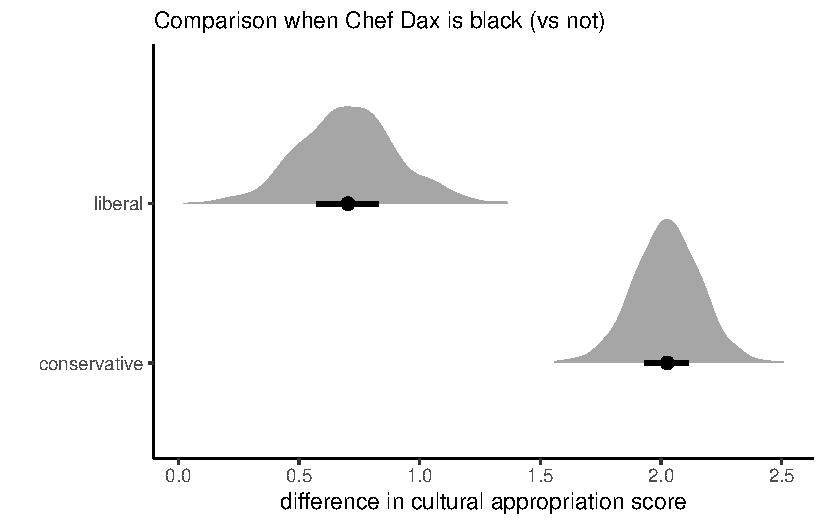
\includegraphics[keepaspectratio]{regression_files/figure-pdf/fig-contrasts-1.pdf}}

}

\caption{\label{fig-contrasts}Difference in appropriation rating for
black vs non-black Chef Dax, average accross different levels of brand
action.}

\end{figure}%

\end{example}

In multivariate regression, it sometimes is useful to specify correlated
coefficients (e.g., for random effects). This leads to the necessity to
set a prior on a covariance matrix.

\begin{proposition}[Wishart
distribution]\protect\hypertarget{prp-Wishart-distribution}{}\label{prp-Wishart-distribution}

Let \(\boldsymbol{Q}\) by a random \(p \times p\) symmetric positive
definite matrix with Wishart distribution, denoted
\(\mathbf{Q} \sim \mathsf{Wishart}_p(\nu, \mathbf{S})\) for \(\nu>0\)
degrees of freedom and scale \(\mathbf{S}\). It's density is
proportional to \begin{align*}
 f(\boldsymbol{Q}) \stackrel{\boldsymbol{Q}}{\propto} |\boldsymbol{Q}|^{(\nu-p-1)/2}\exp\{-\mathrm{tr}(\mathbf{S}^{-1}\boldsymbol{Q})/2\}, \qquad \nu > p-1.
\end{align*} where \(|\cdot|\) denotes the determinant of the matrix and
\(\mathrm{tr}\) the trace operator. The Wishart also arises from
considering \(n \geq p\) independent and identically distributed mean
zero Gaussian vectors
\(\boldsymbol{Y}_i \sim \mathsf{Gauss}_p(\boldsymbol{0}_p, \mathbf{S})\),
where \begin{align*}
 \sum_{i=1}^{\nu} \boldsymbol{Y}_i\boldsymbol{Y}_i^\top \sim \mathsf{Wishart}_p(\nu, \mathbf{S}).
\end{align*} For prior elicitation, \(\nu\) is thus a prior sample size,
whereas we can specify \(\mathbf{S}\) using the fact that the mean of
the Wishart is \(\nu \mathbf{S}\); taking an identity matrix is
standard. For more mathematical properties, consult Chapter 8 of Eaton
(\citeproc{ref-Eaton:2007}{2007}).

\end{proposition}

\begin{definition}[Inverse
Wishart]\protect\hypertarget{def-inverse-wishart}{}\label{def-inverse-wishart}

Analogous to the relationship between gamma prior for the precision and
inverse gamma for the variance, we can also similarly consider a prior
for the covariance matrix \(\boldsymbol{\Sigma} = \boldsymbol{Q}^{-1}\).
Applying the change of variable formula, we get Jacobian
\(|\boldsymbol{\Sigma}|^{p+1}\), and so \(\boldsymbol{\Sigma}\) is
inverse Wishart \(\mathsf{inv. Wishart}(\nu, \mathbf{S}^{-1}),\) with
density proportional to \begin{align*}
 p(\boldsymbol{\Sigma}) \propto |\boldsymbol{\Sigma}|^{-(\nu+p+1)/2} \exp\left\{-\frac{1}{2} \mathrm{tr}\left(\boldsymbol{S}^{-1}\boldsymbol{\Sigma}^{-1}\right)\right\}
\end{align*} with expectation \(\mathbf{S}^{-1}(\nu-p-1)\) for
\(\nu > p+1.\)

\end{definition}

\begin{proposition}[Wishart as conjugate prior in Gaussian
model]\protect\hypertarget{prp-conjugate-prior}{}\label{prp-conjugate-prior}

Consider
\(\boldsymbol{\mu} \sim \mathsf{Gauss}_p(\boldsymbol{\mu}_0, \boldsymbol{Q}^{-1})\)
and \(\boldsymbol{Q} \sim \mathsf{Wishart}_p(\nu, \mathbf{S})\) for
\(\nu \geq p\). Then, the conditional density of
\(\boldsymbol{Q} \mid \boldsymbol{\mu}, \boldsymbol{\mu}_0\) is
proportional to \begin{align*}
 |\boldsymbol{Q}|^{1/2} \exp \left\{ -\frac{1}{2} (\boldsymbol{\mu}-\boldsymbol{\mu}_0)^\top\boldsymbol{Q}(\boldsymbol{\mu}-\boldsymbol{\mu}_0)\right\} |\boldsymbol{Q}|^{(\nu-p-1)/2}\exp\{-\mathrm{tr}(\mathbf{S}^{-1}\boldsymbol{Q})/2\}
\end{align*} and thus
\(\mathsf{Wishart}_p\{\nu + 1/2, \boldsymbol{S} + (\boldsymbol{\mu}-\boldsymbol{\mu}_0)(\boldsymbol{\mu}-\boldsymbol{\mu}_0)^\top\}.\)
To see this, note that a \(1 \times 1\) matrix is equal to it's trace,
and the trace operator is invariant to cyclic of it's argument, meaning
that \begin{align*}
 (\boldsymbol{\mu}-\boldsymbol{\mu}_0)^\top\boldsymbol{Q}(\boldsymbol{\mu}-\boldsymbol{\mu}_0) = \mathrm{tr}\left\{ \boldsymbol{Q}(\boldsymbol{\mu}-\boldsymbol{\mu}_0)(\boldsymbol{\mu}-\boldsymbol{\mu}_0)^\top\right\}.
\end{align*} We then combine elements to get the parameters. This
extends naturally to the case of \(n\) independent observations, for
example linear regression model.

\end{proposition}

\begin{proposition}[Priors for variance
matrices]\protect\hypertarget{prp-prior-variance}{}\label{prp-prior-variance}

The marginal precision for the Wishart variate are gamma distributed
with the same degrees of freedom \(\nu\). The problem with using this
prior is that it has a single parameter governing all scale parameters
(i.e., the marginal variance) and the absolute value of the correlation
and marginal variance parameters are negatively related
(\citeproc{ref-Gelman:2013}{Gelman et al. 2013}), as seen in
Figure~\ref{fig-draws-Wishart}. Large variance thus correspond to small
correlations shrunk towards zero when the degrees of freedom increase.
There exists alternative distributions, such as the scaled-inverse
Wishart, that add redundant scale parameters to decouple
\(\mathrm{diag}(\boldsymbol{\xi}) \times \boldsymbol{\Sigma} \times \mathrm{diag}(\boldsymbol{\xi})\),
but we refrain from pursuing these here.

\begin{figure}[ht!]

\centering{

\pandocbounded{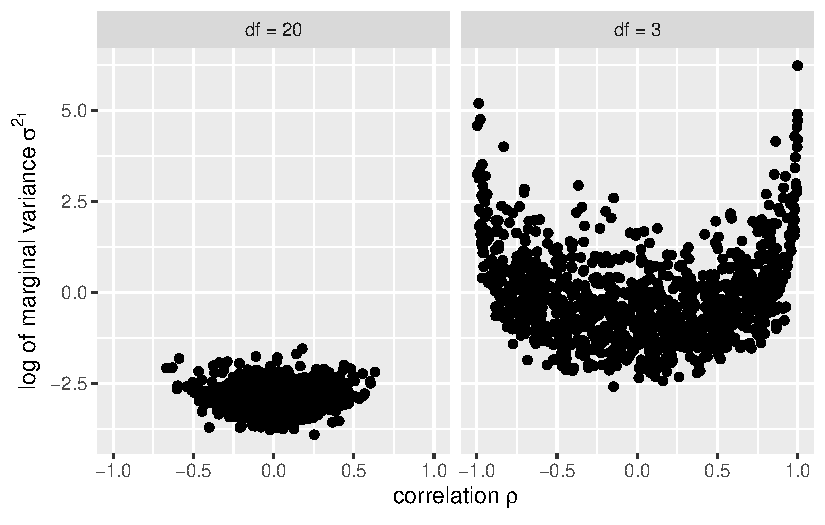
\includegraphics[keepaspectratio]{regression_files/figure-pdf/fig-draws-Wishart-1.pdf}}

}

\caption{\label{fig-draws-Wishart}Prior draws from a bivariate inverse
Wishart with identity scale matrix and \(\nu \in \{3, 20\}\) degrees of
freedom.}

\end{figure}%

A better alternative is to specify different prior for each marginal
scale \(\sigma_j\) and a prior on the correlation matrix \(\mathbf{R}.\)
For the latter, the onion peel or LKJ prior, named after the authors of
Lewandowski, Kurowicka, and Joe (\citeproc{ref-Lewandowski:2009}{2009}),
is \(p(\mathbf{R}) \propto |\mathbf{R}|^{\eta-1}\) for a scale
\(\eta>0.\) The case \(\eta=1\) leads to uniform over the space of
correlation matrices, and \(\eta>1\) favours the identity matrix.

\end{proposition}

\section{Shrinkage priors}\label{shrinkage-priors}

In contexts where the number of regressors \(p\) is considerable
relative to the sample size \(n\), it may be useful to constrain the
parameter vector if we assume that the signal is sparse, with a large
proportion of coefficients that should be zero. This is notably
important when the ratio \(p/n \to c\) for \(c > 0,\) meaning that the
number of coefficients and covariates increases proportional to the
sample size. Shrinkage priors can regularize and typically consist of
distributions that have a mode at zero, and another that allows for
larger signals.

In the Bayesian paradigm, regularization is achieved via priors that
have mass at or towards zero, pushing coefficients of the regression
model towards zero unless there is strong evidence from the likelihood
against this. We however want to allow non-zero coefficients, typically
by setting coefficient-specific parameters with a heavy tailed
distribution to prevent overshrinking. Most if not all parameter can be
viewed as scale mixtures of Gaussian.

We make a distinction between \textbf{global} shrinkage priors those
that consider a common shrinkage parameter for all regression
coefficients, to be compared with \textbf{local} scale mixtures that
have coefficient-specific parameters.

The scale parameters and hyperparameters can be estimated jointly with
the model, and uncertainty diagnostics follow naturally. We assume that
coefficients \(\beta_j\) are independent apriori, although it is
possible to specify group structures (e.g., for handling coefficients
associated to a common categorical covariate with \(K\) levels,
represented by \(K-1\) columns of dummy group indicators).

\begin{proposition}[Spike-and-slab
prior]\protect\hypertarget{prp-spike-slab}{}\label{prp-spike-slab}

The spike-and-slab prior is a two-component mixture with that assigns a
positive probability to zero via a point mass \(\delta_0\) or a vary
narrow distribution centered at the origin (the spike) and the balance
to the slab, a diffuse distribution.

The spike-and-slab prior was originally proposed by Mitchell and
Beauchamp (\citeproc{ref-Mitchell.Beauchamp:1988}{1988}) with a uniform
on a large interval and a point mass at zero. The term was also used in
George and McCulloch (\citeproc{ref-George.McCulloch:1993}{1993}), which
replaced the prior by a mixture of Gaussians, one of which diffuse and
the other with near infinite precision and centered at the origin. The
latter is known under the vocable stochastic search variable selection
prior. Letting \(\gamma_j \in [0,1]\) denote the probability of the slab
or inclusion of the variable, the independent priors for the regression
coefficients are \begin{align*}
 \beta_j \mid \gamma_j, \sigma_j^2,\phi^2_j \sim (1-\gamma_j) \mathsf{Gauss}(0, \sigma_j^2\phi^2_j) + \gamma_j \mathsf{Gauss}(0, \phi^2)
\end{align*} where \(\phi^2_j\) is very nearly zero, e.g.,
\(\phi_j^2=0.001.\) The construction allows for variable augmentation
with mixture indicators and Gibbs sampling, although mixing tends to be
poor.

\end{proposition}

\begin{proposition}[Horseshoe
prior]\protect\hypertarget{prp-horseshoe}{}\label{prp-horseshoe}

The horseshoe prior of Carvalho, Polson, and Scott
(\citeproc{ref-Carvalho.Polson.Scott:2010}{2010}) is a hierarchical
prior of the form \begin{align*}
\beta_j \mid \sigma^2_j \sim \mathsf{Gauss}(0, \sigma^2_j), \quad \sigma^2_j \mid \lambda \sim \mathsf{Student}_{+}(0, \lambda, 1), \quad \lambda \sim \mathsf{Student}_{+}(0, \omega, 1)
\end{align*} where \(\mathsf{Student}_{+}(0, a, 1)\) denotes a
half-Cauchy distribution with scale \(a>0,\) truncated on
\(\mathbb{R}_{+}.\)

This prior has no explicit density, but is continuous and can be
simulated. It is useful to consider the behaviour of the random variance
\(\sigma^2_j\) term, which leads to an unconditional scale mixture of
Gaussian for \(\beta_j\). More useful to understanding is looking at
\(\kappa = 1 - 1/(1+\sigma^2)\), which gives a weight in \([0,1].\) We
can see what happens to the shrunk components close to zero by looking
at the density of \(\kappa \to 0\), and similarly at the large signals
when \(\kappa \to 1.\) The Cauchy prior does not shrink towards zero,
and lets large signals pass, whereas the Bayesian LASSO double
exponential shrinkage leads to attenuation of strong signals. The
horseshoe prior name comes from the shape of the prior, which leads to a
shrinkage analog to \(\mathsf{beta}(1/2, 1/2)\) and thus penalizes,
forcing components to be either large or small.

Figure~\ref{fig-weights-shrinkage} shows the weighting implied by the
mixture density for a Cauchy prior on the variance, the double
exponential of the Laplace from Bayesian LASSO and the horseshoe.

\begin{figure}[ht!]

\centering{

\pandocbounded{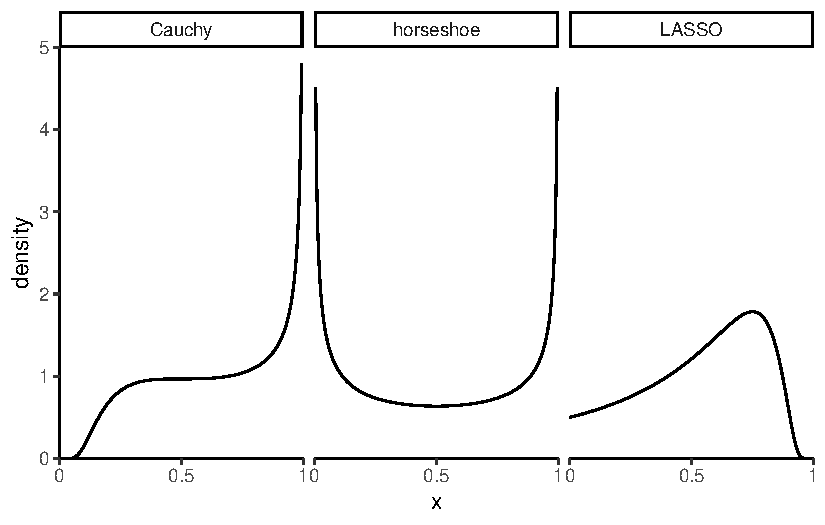
\includegraphics[keepaspectratio]{regression_files/figure-pdf/fig-weights-shrinkage-1.pdf}}

}

\caption{\label{fig-weights-shrinkage}Density of penalization weights
\(\kappa\) of spike (near zero) and slab (near one) for three shrinkage
priors.}

\end{figure}%

\end{proposition}

\begin{figure}[ht!]

\centering{

\pandocbounded{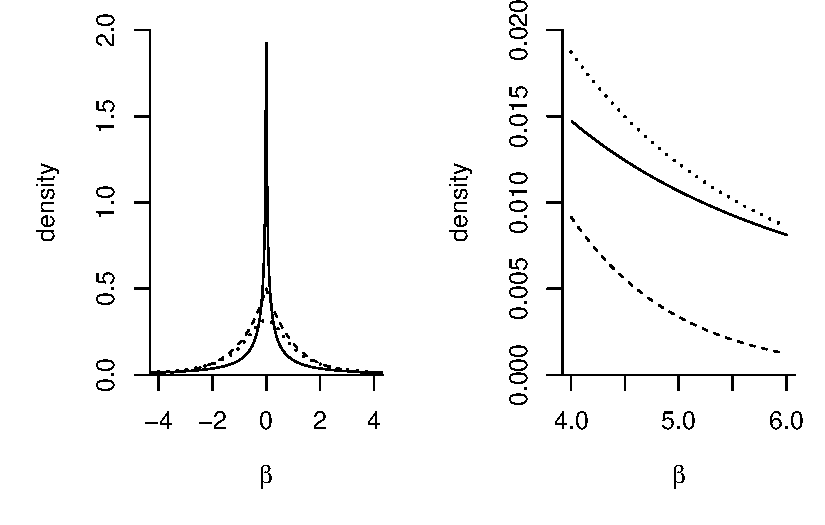
\includegraphics[keepaspectratio]{regression_files/figure-pdf/fig-shrinkage-1.pdf}}

}

\caption{\label{fig-shrinkage}Marginal density for a regression
coefficient \(\beta\) with horseshoe prior (full), Laplace (dashed) and
a Student-\(t\) (thick dotted). The plot on the right shows the tail
behaviour. The density of the horseshoe is unbounded at the origin.
Inspired from Figure 1 of Carvalho, Polson, and Scott
(\citeproc{ref-Carvalho.Polson.Scott:2010}{2010}).}

\end{figure}%

While the horseshoe prior guarantees that large coefficients are not
regularized, this feature of the shrinkage prior is harmful in certain
instances, for example separation of variables for logistic regression.
Markov chain Monte Carlo simulations are hampered by these parameters
whose posterior mean does not exist, leading to poor mixing. Some very
weak regularization for these big components can thus help. Piironen and
Vehtari (\citeproc{ref-Piironen.Vehtari:2017}{2017}) proposed the
regularized horseshoe, nicknamed Finnish horseshoe, where \begin{align*}
\beta_j \mid \lambda, \tau_j, c^2 &\sim \mathsf{Gauss}\left(0, \lambda\frac{c^2\tau_j^2}{c^2 + \tau^2_j\lambda^2}\right), \\
\tau_j &\sim \mathsf{Student}_{+}(0, 1, 1)\\
c^2 \mid s^2, \nu &\sim \mathsf{inv. gamma}(\nu/2, \nu s^2/2).
\end{align*} When \(\tau^2\lambda^2_j\) is much greater than \(c^2\),
this amounts to having a Student slab with \(\nu\) degrees of freedom
for large coefficients; taking a small value of \(\nu\) allows for
large, but not extreme components, and the authors use \(s^2=2, \nu=4.\)
The above specification does not specify the prior for the global scale
\(\lambda\), for which Piironen and Vehtari
(\citeproc{ref-Piironen.Vehtari:2017}{2017}) recommend using an
empirical Bayes prior, with
\[\lambda \sim \mathsf{Student}_{+}\left\{0, \frac{p_0}{(p-p_0)}\frac{\sigma}{n^{1/2}}, 1\right\},\]
where \(p_0\) is a prior guess for the number of non-zero components out
of \(p,\) \(n\) is the sample size and \(\sigma\) is some level of the
noise.

\begin{example}[Comparison of shrinkage
priors]\protect\hypertarget{exm-case-study-shrinkage}{}\label{exm-case-study-shrinkage}

We revisit the \texttt{diabetes} data from the \textbf{R} package
\texttt{lars}, which was used in Park and Casella
(\citeproc{ref-Park.Casella:2008}{2008}) to illustrate the Bayesian
LASSO. We consider three methods: the default Gaussian prior, which
gives a ridge penalty, the Bayesian LASSO and finally the horseshoe.
Models are fitted using the \texttt{bayesreg} package.

Figure~\ref{fig-shrinkage-dens-comparison} shows the ordered
coefficients for each method. We can see that the ridge has the widest
intervals of all methods, providing some shrinkage only for large values
of \(\beta\). The horseshoe has typically narrower intervals, with more
mass in a neighborhood of zero for smaller coefficients, and asymmetric
intervals.

\begin{figure}[ht!]

\centering{

\pandocbounded{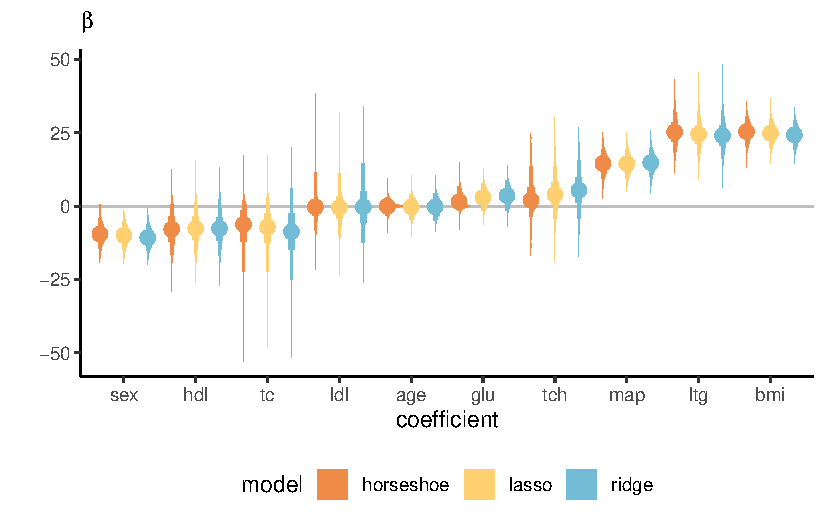
\includegraphics[keepaspectratio]{regression_files/figure-pdf/fig-shrinkage-dens-comparison-1.pdf}}

}

\caption{\label{fig-shrinkage-dens-comparison}Density estimates for
regression coefficients with Gaussian (ridge), double exponential
(Laplace) and horseshoe priors for the \texttt{diabetes} data.}

\end{figure}%

One aspect worth mentioning is that the horseshoe prior impacts strongly
the geometry and leads to slower mixing than the conjugate or
Student-\(t\) priors: the effective sample size fraction relative to the
number of samples ranges from 15\% to 100\%, compared to 50\% to 96\%
for the Bayesian LASSO and near-independent draws with the conjugate
ridge.

\end{example}

\section{Bayesian model averaging via reversible
jump}\label{bayesian-model-averaging-via-reversible-jump}

Variable selection refers to selection of covariates from a set of \(p\)
candidates from a design matrix which is orthogonal to the intercept;
these could include higher order terms or interactions. From the
Bayesian perspective, all of these \(2^p-1\) submodels must be assigned
a prior. We can also rule out models without lower order interactions
through the prior, but exploring or fitting all possible models is too
costly. The goal of the analysis is to account for the uncertainty
associated with variable selection. The target of inference is often the
weight of the combinations, and the probability that a predictor is
included aposteriori.

There are different methods for doing this: one is through spike and
slab priors. Software for Hamiltonian Monte Carlo like Stan cannot
handle discrete variables. Other methods for Bayesian model averaging
includes use of reversible jump Markov chain Monte Carlo
(\citeproc{ref-Green:1995}{Green 1995}), an extension that allows for
arbitrary measures and through this varying dimensions, which occurs not
only with variable selection, but also changepoint analysis and mixture
models with varying number of components
(\citeproc{ref-Green:2001}{Green 2001}). Reversible jump requires a form
of data augmentation to have dimension-balancing and defining different
types of moves for jumping between dimensions. These are integrated in
the Metropolis--Hastings step through a Jacobian term added to \(R\).
with different types of moves giving termed padding andone to pad the
dimensions to match and define. In regression models, we will consider
moves that adds or removes one parameter/regressor at a time.

Consider the setup of Proposition~\ref{prp-gaussian-ols}, where we
consider models \(M_1, \ldots, M_m\) with for simplicity \(p(M_i)=1\)
for all models that include an intercept. We define \(\mathbf{X}^{(m)}\)
and \(\boldsymbol{\beta}^{(m)}\) as the model matrix and the associated
vector of non-zero coefficients associated with it. Let the response
vector \begin{align*}
\boldsymbol{Y} \mid M_m, \boldsymbol{\beta}, \sim \mathsf{Gauss}(\mathbf{X}^{(m)}\boldsymbol{\beta}^{(m)}, \boldsymbol{\Sigma})    
\end{align*} where \(\boldsymbol{\beta}^{(m)} \mid M_m,\) is assigned a
Gaussian prior, and likewise the covariance parameters are given
suitable priors. We write \(|M|\) for the cardinality of the set of
non-zero coefficients \(\boldsymbol{\beta}\) in model \(M.\)

Write \(\boldsymbol{\theta}\) for all parameters other than the
response, model and vector of coefficients. We can consider a joint
update of the regression parameters \(\boldsymbol{\beta}, M\) by
sampling from their joint distribution via
\(p(\boldsymbol{\beta} \mid M, \boldsymbol{\theta}) p(M \mid \boldsymbol{\theta}).\)
The update for the coefficients
\(p(\boldsymbol{\beta} \mid M, \boldsymbol{\theta})\) is as usual, while
for \(p(M \mid \boldsymbol{\theta})\), we get the conditional Bayes
factor, \begin{align*}
 p(M \mid \boldsymbol{Y}, \boldsymbol{\theta}) &\stackrel{M}{\propto} p(M) p(\boldsymbol{Y} \mid M, \boldsymbol{\theta})
 \\&= p(M) \int_{\mathbb{R}^{\mathbb{|M|}}}p(\boldsymbol{Y} \mid M, \boldsymbol{\beta},\boldsymbol{\theta}) p(\boldsymbol{\beta} \mid M, \boldsymbol{\theta}) d \boldsymbol{\beta}
\end{align*} We can marginalize out \(\boldsymbol{\beta}\) and show
(demonstration omitted) that \begin{align*}
p(\boldsymbol{M} \mid \boldsymbol{Y}, \boldsymbol{\theta}) \propto p(M) |\boldsymbol{Q}_{\boldsymbol{\beta}}|^{-1/2}\exp\left( \frac{1}{2} \boldsymbol{\mu}_{\boldsymbol{\beta}}^\top\boldsymbol{Q}_{\boldsymbol{\beta}} \boldsymbol{\mu}_{\boldsymbol{\beta}}\right)
\end{align*} where \(\boldsymbol{\mu}_{\boldsymbol{\beta}}\) and
\(\boldsymbol{Q}_{\boldsymbol{\beta}}\) are the mean and precision of
\(p(\boldsymbol{\beta} \mid \boldsymbol{Y}, M, \boldsymbol{\theta}).\)

We then consider different types of move for the \(k_{\max}\) potential
covariates (including interactions, etc.)
(\citeproc{ref-Holmes:2002}{Holmes, Denison, and Mallick 2002})

\begin{itemize}
\tightlist
\item
  expansion: adding an unused covariate chosen at random from the
  remaining ones
\item
  shrinkage: removing one covariate at random from the current matrix
\item
  swapping an active covariate for an unused one.
\end{itemize}

Only the last type of move preserves the dimension, whereas the
shrinkage and expansion moves lead to a decrease or increase of the
model matrix dimension. The probability of rejection for Metropolis
becomes \begin{align*}
R = J\frac{p(\boldsymbol{\theta}_t^{\star})}{p(\boldsymbol{\theta}_{t-1})}\frac{q(\boldsymbol{\theta}_{t-1} \mid \boldsymbol{\theta}_t^{\star} )}{q(\boldsymbol{\theta}_t^{\star} \mid \boldsymbol{\theta}_{t-1})}
\end{align*} where for most moves \(J=1\) in this case, except in four
cases where the dimension \(|M| \in\{1, 2, k_{\max}-1, k_{\max}\}\) and

\begin{itemize}
\tightlist
\item
  \(J=2/3\) if \(|M|=1\) and we try to add a covariate
\item
  \(J=2/3\) if \(|M|=k_{\max}\) and we try to remove a covariate
\item
  \(J=3/2\) if \(|M|=2\) and we try to remove a covariate
\item
  \(J=3/2\) if \(|M|=k_{\max}-1\) and we try to add the last covariate.
\end{itemize}

The move for \(M\) is accepted as usual if the drawn uniform
\(U \sim \mathsf{unif}(0,1)\) satisfies \(U<R\).

\bookmarksetup{startatroot}

\chapter{Gaussian approximations}\label{gaussian-approximations}

So far, we have focused on stochastic approximations of integral. In
very large models, Markov chain Monte Carlo suffer from the curse of
dimensionality and it is sometimes useful to resort to cheaper
approximations. We begin this review by looking at the asymptotic
Gaussian limiting distribution of the maximum aposteriori, the Laplace
approximations for integrals (\citeproc{ref-Tierney.Kadane:1986}{Tierney
and Kadane 1986}), and their applications for model comparison
(\citeproc{ref-Raftery:1995}{Raftery 1995}) and evaluation of the
marginal likelihood. We also discuss integrated nested Laplace
approximations (\citeproc{ref-Rue.Martino.Chopin:2009}{Håvard Rue,
Martino, and Chopin 2009}; \citeproc{ref-Wood:2019}{Wood 2019}), used in
hierarchical models with Gaussian components to obtain approximations to
the marginal distribution. This material also borrows from Section 8.2
and appendix C.2.2 of Held and Bové
(\citeproc{ref-Held.Bove:2020}{2020}).

We make use of Landau's notation to describe the growth rate of some
functions: we write \(x = \mathrm{O}(n)\) (big-O) to indicate that the
ratio \(x/n \to c \in \mathbb{R}\) and \(x =\mathrm{o}(n)\) when
\(x/n \to 0,\) both when \(n \to \infty.\)

\section{Laplace approximation and it's
applications}\label{laplace-approximation-and-its-applications}

\begin{proposition}[Laplace approximation for
integrals]\protect\hypertarget{prp-Laplace-approximation}{}\label{prp-Laplace-approximation}

The Laplace approximation uses a Gaussian approximation to evaluate
integrals of the form \begin{align*}
I_n= \int_a^b g(x) \mathrm{d} x =\int_a^b  \exp\{nh(x)\}\mathrm{d} x.
\end{align*} Assume that \(g(x)\) and thus \(h(x),\) is concave and and
twice differentiable, with a maximum at \(x_0 \in [a,b].\) We can Taylor
expand \(h(x)\) to get, \begin{align*}
h(x) = h(x_0) + h'(x_0)(x-x_0) + h''(x_0)(x-x_0)^2/2 + R
\end{align*} where the remainder \(R=\mathrm{O}\{(x-x_0)^3\}.\) If
\(x_0\) is a maximizer and solves \(h'(x_0)=0,\) then letting
\(\tau=-nh''(x_0),\) we can write ignoring the remainder term the
approximation \begin{align*}
 I_n &\approx \exp\{nh(x_0)\} \int_{a}^b \exp \left\{-\frac{1}{2}(x-x_0)^2\right\}
  \\&= \exp\{nh(x_0)\} \left(\frac{2\pi}{\tau}\right)^{1/2} \left[\Phi\left\{ \tau(b-x_0)\right\} - \Phi\left\{\tau(a-x_0)\right\}\right]
\end{align*} upon recovering the unnormalized kernel of a Gaussian
random variable centered at \(x_0\) with precision \(\tau.\) The
approximation error is \(\mathrm{O}(n^{-1}).\)

The multivariate analog is similar, where now for an integral of the
form \(\exp\{nh(\boldsymbol{x})\}\) over a subset of \(\mathbb{R}^d,\)
we consider the Taylor series expansion \begin{align*}
 h(\boldsymbol{x}) &= h(\boldsymbol{x}_0) + (\boldsymbol{x}- \boldsymbol{x}_0)^\top h'(\boldsymbol{x}_0) + \frac{1}{2}(\boldsymbol{x}- \boldsymbol{x}_0)^\top h''(\boldsymbol{x}_0)(\boldsymbol{x}- \boldsymbol{x}_0) + R.
\end{align*} We obtain the Laplace approximation at the mode
\(\boldsymbol{x}_0\) satisfying
\(h'(\boldsymbol{x}_0)=\boldsymbol{0}_d,\) \begin{align*}
 I_n \approx \left(\frac{2\pi}{n}\right)^{p/2} | \mathbf{H}(\boldsymbol{x}_0)|^{-1/2}\exp\{nh(\boldsymbol{x}_0)\},
\end{align*} where \(|\mathbf{H}(\boldsymbol{x}_0)|\) is the determinant
of the Hessian matrix of \(-h(\boldsymbol{x})\) evaluated at the mode
\(\boldsymbol{x}_0.\)

\end{proposition}

Laplace approximation uses a Taylor series approximation to approximate
the density, but since the latter must be non-negative, it performs the
approximation on the log scale and back-transform the result. It is
important to understand that we can replace \(nh(\boldsymbol{x})\) by
any \(\mathrm{O}(n)\) term.

\begin{corollary}[Laplace approximation for marginal
likelihood]\protect\hypertarget{cor-laplace-loglik}{}\label{cor-laplace-loglik}

Consider a simple random sample \(\boldsymbol{Y}\) of size \(n\) from a
distribution with parameter vector
\(\boldsymbol{\theta} \in \mathbb{R}^p.\) We are interested in
approximating the marginal likelihood for a parametric model with
\(\boldsymbol{\theta} \in \mathbb{R}^d.\) Write
(\citeproc{ref-Raftery:1995}{Raftery 1995}) \begin{align*}
 p(\boldsymbol{y}) = \int_{\mathbb{R}^d} p(\boldsymbol{y} \mid \boldsymbol{\theta}) p(\boldsymbol{\theta}) \mathrm{d} \boldsymbol{\theta}
\end{align*} and take
\begin{align*}nh(\boldsymbol{\theta}) = \log p(\boldsymbol{y} \mid \boldsymbol{\theta}) + \log p(\boldsymbol{\theta})
\end{align*} in Proposition~\ref{prp-Laplace-approximation}. Then,
evaluating at the maximum a posteriori
\(\widehat{\boldsymbol{\theta}}_{\mathrm{MAP}},\) we get \begin{align*}
 p(\boldsymbol{y}) = p(\widehat{\boldsymbol{\theta}}_{\mathrm{MAP}})p(\boldsymbol{y} \mid \widehat{\boldsymbol{\theta}}_{\mathrm{MAP}}) (2\pi)^{d/2}|\mathbf{H}(\widehat{\boldsymbol{\theta}}_{\mathrm{MAP}})|^{-1/2} + \mathrm{O}(n^{-1})
\end{align*} where \(-\mathbf{H}\) is the Hessian matrix of second
partial derivatives of the unnormalized log posterior. We get the same
relationship on the log scale, whence
(\citeproc{ref-Tierney.Kadane:1986}{Tierney and Kadane 1986})
\begin{align*}
 \log p(\boldsymbol{y}) = \log p(\widehat{\boldsymbol{\theta}}_{\mathrm{MAP}}) + \log p(\boldsymbol{y} \mid \widehat{\boldsymbol{\theta}}_{\mathrm{MAP}}) + \frac{d}{2} \log (2\pi) - \frac{1}{2}\log |\mathbf{H}(\widehat{\boldsymbol{\theta}}_{\mathrm{MAP}})| + \mathrm{O}(n^{-1})
\end{align*} If \(p(\boldsymbol{\theta}) = \mathrm{O}(1)\) and
\(p(\boldsymbol{y} \mid \boldsymbol{\theta}) = \mathrm{O}(n)\) and
provided the prior does not impose unnecessary support constraints, we
get the same limiting approximation if we replace the maximum a
posteriori point estimator
\(\widehat{\boldsymbol{\theta}}_{\mathrm{MAP}}\) by the maximum
likelihood estimator, and
\(-\mathbf{H}(\widehat{\boldsymbol{\theta}}_{\mathrm{MAP}})\) by
\(n\boldsymbol{\imath},\) where \(\boldsymbol{\imath}\) denotes the
Fisher information matrix for a sample of size one. We can write the
determinant of the \(n\)-sample Fisher information as
\(n^{d}|\boldsymbol{\imath}|.\)

If we use this approximation instead, we get \begin{align*}
 \log p(\boldsymbol{y}) &= \log p(\boldsymbol{y} \mid \widehat{\boldsymbol{\theta}}_{\mathrm{MLE}}) -\frac{d}{2} \log n + \\& \quad  \log p(\widehat{\boldsymbol{\theta}}_{\mathrm{MLE}}) - \frac{1}{2} \log |\boldsymbol{\imath}| + \frac{d}{2} \log(2\pi)  + \mathrm{O}(n^{-1/2})
\end{align*} where the error is now \(\mathrm{O}(n^{-1/2})\) due to
replacing the true information by the evaluation at the MLE. The
likelihood is \(\mathrm{O}(n),\) the second is \(\mathrm{O}(\log n)\)
and the other three are \(\mathrm{O}(1).\) If we take the prior to be a
multivariate Gaussian with mean \(\boldsymbol{\theta}_{\mathrm{MLE}}\)
and with variance \(\boldsymbol{\imath},\) then the approximation error
is \(\mathrm{O}(n^{-1/2}),\) whereas the marginal likelihood has error
\(\mathrm{O}(1)\) if we only keep the first two terms. This gives the
approximation \begin{align*}
-2\log p(\boldsymbol{y}) \approx \mathsf{BIC} = -2\log p(\boldsymbol{y} \mid \boldsymbol{\theta}) + p\log n
\end{align*} If the likelihood contribution dominates the posterior, the
\(\mathsf{BIC}\) approximation will improve with increasing sample size,
so \(\exp(-\mathsf{BIC}/2)\) is an approximation fo the marginal
likelihood sometimes used for model comparison in Bayes factor, although
this derivation shows that the latter neglects the impact of the prior.

\end{corollary}

\begin{example}[Bayesian model averaging
approximation]\protect\hypertarget{exm-bic-bma}{}\label{exm-bic-bma}

Consider the \texttt{diabetes} model from Park and Casella
(\citeproc{ref-Park.Casella:2008}{2008}). We fit various linear
regression models, considering all best models of a certain type with at
most the 10 predictors plus the intercept. In practice, we typically
restrict attention to models within some distance of the lowest BIC
value, as the weights otherwise will be negligible.

\begin{figure}[ht!]

\centering{

\pandocbounded{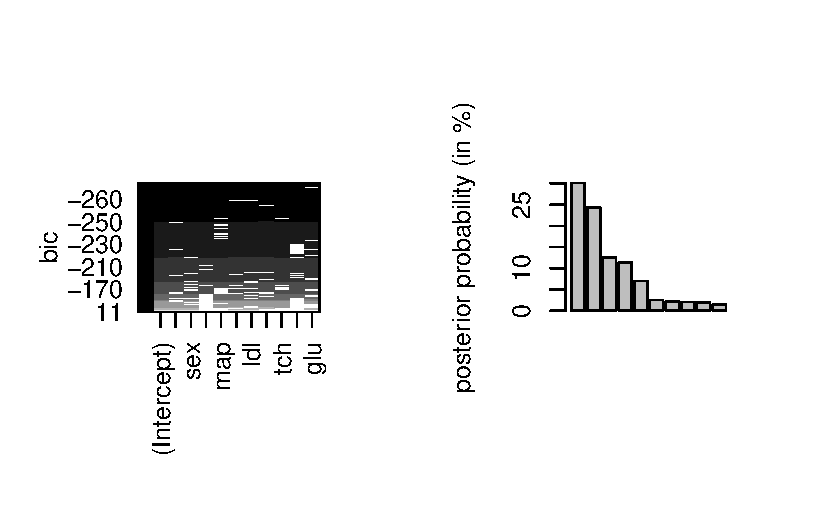
\includegraphics[keepaspectratio]{laplace_files/figure-pdf/fig-bmaweights-1.pdf}}

}

\caption{\label{fig-bmaweights}BIC as a function of the linear model
covariates (left) and Bayesian model averaging approximate weights (in
percentage) for the 10 models with the highest posterior weights
according to the BIC approximation.}

\end{figure}%

Most of the weight is on a handful of complex models, where the best
fitting model only has around \(30\)\% of the posterior mass.

\end{example}

\begin{refremark}[Parametrization for Laplace]
Compare to sampling-based methods, the Laplace approximation requires
optimization to find the maximum of the function. The Laplace
approximation is not invariant to reparametrization: in practice, it is
best to perform it on a scale where the likelihood is as close to
quadratic as possible in \(g(\boldsymbol{\theta})\) and back-transform
using a change of variable.

\label{rem-marginal-lik-laplace}

\end{refremark}

We can also use Laplace approximation to obtain a crude second-order
approximation to the posterior. We suppose that the prior is proper.

We can Taylor expand the log prior and log density around their
respective mode, say \(\widehat{\boldsymbol{\theta}}_0\) and
\(\widehat{\boldsymbol{\theta}}_{\mathrm{MLE}},\) with
\(\jmath_0(\widehat{\boldsymbol{\theta}}_0)\) and
\(\jmath(\widehat{\boldsymbol{\theta}}_{\mathrm{MLE}})\) denoting
negative of the corresponding Hessian matrices evaluated at their mode,
meaning the observed information matrix for the likelihood component.
Together, these yield \begin{align*}
\log p(\boldsymbol{\theta}) &\approx \log p(\widehat{\boldsymbol{\theta}}_0) - \frac{1}{2}(\boldsymbol{\theta} - \widehat{\boldsymbol{\theta}}_0)^\top\jmath_0(\widehat{\boldsymbol{\theta}}_0)(\boldsymbol{\theta} - \widehat{\boldsymbol{\theta}}_0)\\
\log p(\boldsymbol{y} \mid \boldsymbol{\theta}) &\approx \log p(\boldsymbol{y} \mid \boldsymbol{\theta}) - \frac{1}{2}(\boldsymbol{\theta} - \widehat{\boldsymbol{\theta}}_{\mathrm{MLE}})^\top\jmath(\widehat{\boldsymbol{\theta}}_{\mathrm{MLE}})(\boldsymbol{\theta} - \widehat{\boldsymbol{\theta}}_{\mathrm{MLE}})
\end{align*}

In the case of flat prior, the curvature is zero and the prior
contribution vanishes altogether. If we apply now
Proposition~\ref{prp-quadratic-forms} to this unnormalized kernel, we
get that the approximate posterior must be Gaussian with precision
\(\jmath_n^{-1}\) and mean \(\mu_n,\) where \begin{align*}
\jmath_n = \jmath_0(\widehat{\boldsymbol{\theta}}_{0}) + \jmath(\widehat{\boldsymbol{\theta}}_{\mathrm{MLE}})
\boldsymbol{\theta}_n = \jmath_n^{-1}\left\{ \jmath_0(\widehat{\boldsymbol{\theta}}_{0})\widehat{\boldsymbol{\theta}}_{0} + \jmath(\widehat{\boldsymbol{\theta}}_{\mathrm{MLE}})\widehat{\boldsymbol{\theta}}_{\mathrm{MLE}}\right\}
\end{align*} and note that
\(\jmath_0(\widehat{\boldsymbol{\theta}}_{0}) = \mathrm{O}(1),\) whereas
\(\jmath_n\) is \(\mathrm{O}(n).\)

\begin{theorem}[Bernstein-von Mises
theorem]\protect\hypertarget{thm-berstein-von-mises}{}\label{thm-berstein-von-mises}

Consider any estimator asymptotically equivalent to the maximum
likelihood estimator and suppose that the prior is continuous and
positive in a neighborhood of the maximum. Assume further that the
regularity conditions for maximum likelihood estimator holds. Then, in
the limit as \(n \to \infty\) \begin{align*}
\boldsymbol{\theta} \mid \boldsymbol{y} \stackrel{\cdot}{\sim} \mathsf{Gauss}\{ \widehat{\boldsymbol{\theta}}_{\mathrm{MLE}},  \jmath^{-1}(\widehat{\boldsymbol{\theta}}_{\mathrm{MLE}})\}
\end{align*}

\end{theorem}

The conclusions from this result is that, in large samples, the
inference obtained from using likelihood-based inference and Bayesian
methods will be equivalent: credible intervals will also have guaranteed
frequentist coverage.

We can use the statement by replacing the maximum likelihood estimator
and the observed information matrix with variants thereof
(\(\boldsymbol{\theta}_n\) and \(\jmath_n,\) or the Fisher information,
or any Monte Carlo estimate of the posterior mean and covariance). The
differences will be noticeable for small samples, but will vanish as
\(n\) grows.

\begin{example}[Gaussian approximations to the
posterior]\protect\hypertarget{exm-gaussian-approx-gamma}{}\label{exm-gaussian-approx-gamma}

To assess the performance of Laplace approximation, we consider an
exponential likelihood with conjugate gamma prior.

The exponential model \(\mathsf{expo}(\lambda)\) has information
\(i(\lambda)=n/\lambda^2\) and third-order cumulant
\(\ell_3(\lambda) = 2n/\lambda^3.\) If we assign a conjugate prior with
\(\lambda \sim \mathsf{gamma}(a,b),\) the mode of the posterior will be
at \(\widehat{\lambda}_{\mathrm{MAP}}=(n+a-1)/(\sum_{i=1}^n y_i + b).\)

\begin{figure}[ht!]

\centering{

\pandocbounded{\includegraphics[keepaspectratio]{laplace_files/figure-pdf/fig-post-gamma-laplace-1.pdf}}

}

\caption{\label{fig-post-gamma-laplace}Gaussian approximation (dashed)
to the posterior density (full line) of the exponential rate \(\lambda\)
for the \texttt{waiting} dataset with an exponential likelihood and a
gamma prior with \(a=0.01\) and \(b=0.01.\) The plots are based on the
first \(10\) observations (left) and the whole sample of size \(n=62\)
(right).}

\end{figure}%

Let us now use Laplace approximation to obtain an estimate of the
marginal likelihood: the latter is \begin{align*}
p(\boldsymbol{y}) = \frac{\Gamma(n+a)}{\Gamma(a)}\frac{b^a}{\left(b + \sum_{i=1}^n y_i \right)^{n+a}}.
\end{align*}

For the sample of size \(62,\) the exponential model marginal likelihood
is \(-276.5,\) whereas the Laplace approximation gives \(-281.9.\)

\end{example}

\begin{proposition}[Posterior expectation using Laplace
method]\protect\hypertarget{prp-expectation-Laplace}{}\label{prp-expectation-Laplace}

If we are interested in computing the posterior expectation of a
positive real-valued functional
\(g(\boldsymbol{\theta}): \mathbb{R}^d \to \mathbb{R}_{+},\) we may
write \begin{align*}
 \mathsf{E}_{\boldsymbol{\Theta} \mid \boldsymbol{Y}}(g(\boldsymbol{\theta}) \mid \boldsymbol{y}) &=  \frac{\int g(\boldsymbol{\theta}) p(\boldsymbol{y} \mid \boldsymbol{\theta}) p( \boldsymbol{\theta}) \mathrm{d} \boldsymbol{\theta}}{\int p(\boldsymbol{y} \mid \boldsymbol{\theta})p( \boldsymbol{\theta}) \mathrm{d} \boldsymbol{\theta}}
\end{align*} We can apply Laplace's method to both numerator and
denominator. Let \(\widehat{\boldsymbol{\theta}}_g\) and
\(\widehat{\boldsymbol{\theta}}_{\mathrm{MAP}}\) of the integrand of the
numerator and denominator, respectively, and the negative of the Hessian
matrix of the log integrands \begin{align*}
\jmath_g&=  -\frac{\partial^2}{\partial \boldsymbol{\theta}\partial \boldsymbol{\theta}^\top} \left\{ \log g(\boldsymbol{\theta}) + \log p(\boldsymbol{y} \mid \boldsymbol{\theta}) + \log p(\boldsymbol{\theta})\right\}, \\
\jmath &=  -\frac{\partial^2}{\partial \boldsymbol{\theta}\partial \boldsymbol{\theta}^\top} \left\{\log p(\boldsymbol{y} \mid \boldsymbol{\theta}) + \log p(\boldsymbol{\theta})\right\}.
\end{align*} Putting these together \begin{align*}
\mathsf{E}_{\boldsymbol{\Theta} \mid \boldsymbol{Y}}(g(\boldsymbol{\theta}) \mid \boldsymbol{y}) = \frac{|\jmath(\widehat{\boldsymbol{\theta}}_{\mathrm{MAP}})|^{1/2}}{|\jmath_g(\widehat{\boldsymbol{\theta}}_g)|^{1/2}} \frac{g(\widehat{\boldsymbol{\theta}}_g) p(\boldsymbol{y} \mid \widehat{\boldsymbol{\theta}}_g) p( \widehat{\boldsymbol{\theta}}_g)}{p(\boldsymbol{y} \mid \widehat{\boldsymbol{\theta}}_{\mathrm{MAP}}) p(\widehat{\boldsymbol{\theta}}_{\mathrm{MAP}})} + \mathrm{O}(n^{-2})
\end{align*} While the Laplace method has an error
\(\mathrm{O}(n^{-1}),\) the leading order term of the expansion cancel
out from the ratio.

\end{proposition}

\section{Integrated nested Laplace
approximation}\label{integrated-nested-laplace-approximation}

In many high dimensional models, use of MCMC is prohibitively expensive
and fast, yet accurate calculations are important. One class of models
whose special structure is particularly amenable to deterministic
approximations.

Consider a model with response \(\boldsymbol{y}\) which depends on
covariates \(\mathbf{x}\) through a latent Gaussian process; typically
the priors on the coefficients \(\boldsymbol{\beta} \in \mathbb{R}^p.\)
In applications with splines, or space time processes, the prior
precision matrix for \(\boldsymbol{\beta}\) will be sparse with a
Gaussian Markov random field structure. The dimension \(p\) can be
substantial (several thousands) with a comparably low-dimensional
hyperparameter vector \(\boldsymbol{\theta} \in \mathbb{R}^m.\) Interest
typically then lies in marginal parameters \begin{align*}
p(\beta_i \mid \boldsymbol{y}) &= \int p(\beta_i \mid \boldsymbol{\theta}, \boldsymbol{y}) p(\boldsymbol{\theta} \mid \boldsymbol{y}) \mathrm{d} \boldsymbol{\theta}\\
p(\theta_i \mid \boldsymbol{y}) &= \int p(\boldsymbol{\theta} \mid \boldsymbol{y}) \mathrm{d} \boldsymbol{\theta}_{-i}
\end{align*} where \(\boldsymbol{\theta}_{-i}\) denotes the vector of
hyperparameters excluding the \(i\)th element \(\theta_i.\) The INLA
method builds Laplace approximations to the integrands
\(p(\beta_i \mid \boldsymbol{\theta}, \boldsymbol{y})\) and
\(p(\boldsymbol{\theta} \mid \boldsymbol{y}),\) and evaluates the
integral using quadrature rules over a coarse grid of values of
\(\boldsymbol{\theta}.\)

The marginal posterior \(p(\boldsymbol{\theta} \mid \boldsymbol{y})\) is
approximated by writing
\(p(\boldsymbol{\beta}, \boldsymbol{\theta} \mid \boldsymbol{y}) \propto p(\boldsymbol{\beta} \mid \boldsymbol{\theta}, \boldsymbol{y}) p(\boldsymbol{\theta} \mid \boldsymbol{y})\)
and performing a Laplace approximation for fixed value of
\(\boldsymbol{\theta}\) for the term
\(p(\boldsymbol{\beta} \mid \boldsymbol{\theta}, \boldsymbol{y}),\)
whose mode we denote by \(\widehat{\boldsymbol{\beta}}.\) This yields
\begin{align*}
\widetilde{p}(\boldsymbol{\theta} \mid \boldsymbol{y}) \propto \frac{p(\widehat{\boldsymbol{\beta}}, \boldsymbol{\theta} \mid \boldsymbol{y})}{ p_{G}(\widehat{\boldsymbol{\beta}} \mid \boldsymbol{y}, \boldsymbol{\theta})} = \frac{p(\widehat{\boldsymbol{\beta}}, \boldsymbol{\theta} \mid \boldsymbol{y})}{ |\boldsymbol{H}(\widehat{\boldsymbol{\beta}})|^{1/2}}
\end{align*} and the Laplace approximation has kernel
\[p_{G}(\boldsymbol{\beta} \mid \boldsymbol{y}, \boldsymbol{\theta}) \propto |\mathbf{H}|^{1/2}\exp\{-(\boldsymbol{\beta}- \widehat{\boldsymbol{\beta}})^\top \mathbf{H}(\boldsymbol{\beta}- \widehat{\boldsymbol{\beta}})/2\};\]
since it is evaluated at \(\widehat{\boldsymbol{\beta}},\) we retrieve
only the determinant of the negative Hessian of
\(p(\boldsymbol{\beta} \mid \boldsymbol{\theta}, \boldsymbol{y}),\)
namely \(\boldsymbol{H}(\widehat{\boldsymbol{\beta}}).\) Note that the
latter is a function of \(\boldsymbol{\theta}.\)

To obtain \(p(\theta_i \mid \boldsymbol{y})\), we then proceed with

\begin{enumerate}
\def\labelenumi{\arabic{enumi}.}
\tightlist
\item
  finding the mode of
  \(\widetilde{p}(\boldsymbol{\theta} \mid \boldsymbol{y})\) using a
  Newton's method, approximating the gradient and Hessian via finite
  differences.
\item
  Compute the negative Hessian at the mode to get an approximation to
  the covariance of \(\boldsymbol{\theta}.\) Use an eigendecomposition
  to get the principal directions \(\boldsymbol{z}\).
\item
  In each direction of \(\boldsymbol{z}\), consider drops in
  \(\widetilde{p}(\boldsymbol{\theta} \mid \boldsymbol{y})\) as we move
  away from the mode and define a coarse grid based on these, keeping
  points where the difference in
  \(\widetilde{p}(\boldsymbol{\theta} \mid \boldsymbol{y})\) relative to
  the mode is less than some numerical tolerance \(\delta.\)
\item
  Retrieve the marginal by numerical integration using the central
  composition design outline above. We can also use directly avoid the
  integration and use the approximation at the posterior mode of
  \(\widetilde{p}(\boldsymbol{\theta} \mid \boldsymbol{y}).\)
\end{enumerate}

Håvard Rue, Martino, and Chopin
(\citeproc{ref-Rue.Martino.Chopin:2009}{2009}) proceed in an analogous
fashion, but instead working with the marginal for \(\beta_i\) building
an approximation of it based on maximizing
\(\boldsymbol{\beta}_{-i} \mid \beta_i, \boldsymbol{\theta}, \boldsymbol{y}\)
to yield \(\widehat{\boldsymbol{\beta}}_{(i)}\) whose \(i\)th element is
\(\beta_i,\) yielding \begin{align*}
\widetilde{p}(\beta_i \mid \boldsymbol{\theta}, \boldsymbol{y}) \propto \frac{p(\widehat{\boldsymbol{\beta}}_{(i)}, \boldsymbol{\theta} \mid \boldsymbol{y})}{\widetilde{p}(\widehat{\boldsymbol{\beta}}_{(i),-i} \mid \beta_i, \boldsymbol{\theta}, \boldsymbol{y})},
\end{align*} with a suitable renormalization of
\(\widetilde{p}(\widehat{\boldsymbol{\beta}}_{(i),-i} \mid \beta_i, \boldsymbol{\theta}, \boldsymbol{y}).\)
Such approximations are reminiscent of profile likelihood.

While we could use the Laplace approximation
\(p_{G}(\widehat{\boldsymbol{\beta}} \mid \boldsymbol{y}, \boldsymbol{\theta})\)
and marginalize the latter directly, this leads to evaluation of the
Laplace approximation to the density far from the mode, which is often
inaccurate. One challenge is that \(p\) again is very large, so
calculation of the Hessian \(\mathbf{H}\) is very high dimensional and
costly to evaluate. Having to evaluate it repeatedly for each marginal
\(\beta_i\) for \(i=1, \ldots, p\) is prohibitive since it involves
factorizations of \(p \times p\) matrices.

To reduce the computational costs, Håvard Rue, Martino, and Chopin
(\citeproc{ref-Rue.Martino.Chopin:2009}{2009}) propose to use the
approximate mean to avoid optimizing and consider the conditional based
on the conditional of the Gaussian approximation with mean
\(\widehat{\boldsymbol{\beta}}\) and covariance
\(\boldsymbol{\Sigma} = \boldsymbol{H}^{-1}(\widehat{\boldsymbol{\beta}}),\)
\begin{align*}
\boldsymbol{\beta}_{-i} \mid \beta_i, \boldsymbol{\theta}, \boldsymbol{y} \approx \mathsf{Gauss}_{p-1}\left\{\widetilde{\boldsymbol{\beta}}_{(i)} = \widehat{\boldsymbol{\beta}}_{-i} + \boldsymbol{\Sigma}_{i,i}^{-1}\boldsymbol{\Sigma}_{i,-i}(\beta_i - \widehat{\beta}_i, \mathbf{M}^{-1}_{-i,-i}\right\};
\end{align*} cf. Proposition~\ref{prp-conditional-gaussian}. This only
requires a rank-one update. Wood (\citeproc{ref-Wood:2019}{2019})
suggest to use a Newton step to correct
\(\widetilde{\boldsymbol{\beta}}_{(i)},\) starting from the conditional
mean. The second step is to exploit the local dependence on
\(\boldsymbol{\beta}\) using the Markov structure to build an
improvement to the Hessian. Further improvements are proposed in Håvard
Rue, Martino, and Chopin (\citeproc{ref-Rue.Martino.Chopin:2009}{2009}),
who used a simplified Laplace approximation to correct the Gaussian
approximation for location and skewness, a necessary step when the
likelihood itself is not Gaussian. This leads to a Taylor series
approximation to correct the log determinant of the Hessian matrix. Wood
(\citeproc{ref-Wood:2019}{2019}) consider a BFGS update to
\(\mathbf{M}^{-1}_{-i,-i}\) directly, which works less well than the
Taylor expansion near \(\widehat{\beta}_i\), but improves upon when we
move far from this value. Nowadays, the INLA software uses a low-rank
variational correction to Laplace method, proposed in van Niekerk and
Rue (\citeproc{ref-vanNiekerk.Rue:2024}{2024}).

The \texttt{INLA} \href{https://www.r-inla.org/}{\textbf{R} package}
provides an interface to fit models with Gaussian latent random effects.
While the software is particularly popular for spatio-temporal
applications using the SPDE approach, we revisit two examples in the
sequel where we can exploit the Markov structure.

\begin{example}[Stochastic volatility model with
INLA]\protect\hypertarget{exm-stochvol-inla}{}\label{exm-stochvol-inla}

Financial returns \(Y_t\) typically exhibit time-varying variability.
The \textbf{stochastic volatility} model is a parameter-driven model
that specifies \begin{align*}
Y_t &= \exp(h_t/2) Z_t \\
h_t &= \gamma + \phi (h_{t-1} - \gamma) + \sigma U_t
\end{align*} where
\(U_t \stackrel{\mathrm{iid}}{\sim} \mathsf{Gauss}(0,1)\) and
\(Z_t \sim  \stackrel{\mathrm{iid}}{\sim} \mathsf{Gauss}(0,1).\) The
\href{https://inla.r-inla-download.org/r-inla.org/doc/likelihood/stochvolgaussian.pdf}{\texttt{INLA}
documentation} provides information about which default prior and
hyperparameters are specified. We use a \(\mathsf{gamma}(1, 0.001)\)
prior for the precision.

\begin{Shaded}
\begin{Highlighting}[]
\FunctionTok{library}\NormalTok{(INLA)}
\CommentTok{\# Stochastic volatility model}
\FunctionTok{data}\NormalTok{(exchangerate, }\AttributeTok{package =} \StringTok{"hecbayes"}\NormalTok{)}
\CommentTok{\# Compute response from raw spot exchange rates at noon}
\NormalTok{y }\OtherTok{\textless{}{-}} \DecValTok{100}\SpecialCharTok{*}\FunctionTok{diff}\NormalTok{(}\FunctionTok{log}\NormalTok{(exchangerate}\SpecialCharTok{$}\NormalTok{rate))}
\CommentTok{\# \textquotesingle{}y\textquotesingle{} is now a series of percentage of log daily differences}
\NormalTok{time }\OtherTok{\textless{}{-}} \FunctionTok{seq\_along}\NormalTok{(y)}
\NormalTok{data }\OtherTok{\textless{}{-}} \FunctionTok{data.frame}\NormalTok{(}\AttributeTok{y =}\NormalTok{ y, }\AttributeTok{time =}\NormalTok{ time)}
\CommentTok{\# Stochastic volatility model}
\CommentTok{\# https://inla.r{-}inla{-}download.org/r{-}inla.org/doc/likelihood/stochvolgaussian.pdf}
\CommentTok{\# The model uses a log link, and a (log){-}gamma prior for the precision}
\NormalTok{f\_stochvol }\OtherTok{\textless{}{-}} \FunctionTok{formula}\NormalTok{(y }\SpecialCharTok{\textasciitilde{}} \FunctionTok{f}\NormalTok{(time, }\AttributeTok{model =} \StringTok{"ar1"}\NormalTok{, }\AttributeTok{param =} \FunctionTok{list}\NormalTok{(}\AttributeTok{prec =} \FunctionTok{c}\NormalTok{(}\DecValTok{1}\NormalTok{, }\FloatTok{0.001}\NormalTok{))))}
\NormalTok{mod\_stochvol }\OtherTok{\textless{}{-}} \FunctionTok{inla}\NormalTok{(f\_stochvol, }\AttributeTok{family =} \StringTok{"stochvol"}\NormalTok{, }\AttributeTok{data =}\NormalTok{ data)}
\CommentTok{\# Obtain summary}
\NormalTok{summary }\OtherTok{\textless{}{-}} \FunctionTok{summary}\NormalTok{(mod\_stochvol)}
\CommentTok{\# plot(mod\_stochvol)}
\NormalTok{marg\_prec }\OtherTok{\textless{}{-}}\NormalTok{ mod\_stochvol}\SpecialCharTok{$}\NormalTok{marginals.hyperpar[[}\DecValTok{1}\NormalTok{]]}
\NormalTok{marg\_phi }\OtherTok{\textless{}{-}}\NormalTok{ mod\_stochvol}\SpecialCharTok{$}\NormalTok{marginals.hyperpar[[}\DecValTok{2}\NormalTok{]]}
\end{Highlighting}
\end{Shaded}

\begin{figure}[ht!]

\centering{

\pandocbounded{\includegraphics[keepaspectratio]{laplace_files/figure-pdf/fig-stochvol-inla-1.pdf}}

}

\caption{\label{fig-stochvol-inla}Marginal densities of precision and
autocorrelation parameters from the Gaussian stochastic volatility
model.}

\end{figure}%

Figure~\ref{fig-stochvol-inla} shows that the correlation \(\phi\) is
nearly one, leading to random walk behaviour and high persistence over
time (this is also due to the frequency of observations). This strong
serial dependence in the variance is in part responsible for the
difficulty in fitting this model using MCMC.

We can use the marginal density approximations to obtain quantiles for
summary of interest. The software also includes utilities to transform
the parameters using the change of variable formula.

\begin{Shaded}
\begin{Highlighting}[]
\CommentTok{\# Compute density, quantiles, etc. via inla.*marginal}
\DocumentationTok{\#\# approximate 95\% credible interval and marginal post median}
\NormalTok{INLA}\SpecialCharTok{::}\FunctionTok{inla.qmarginal}\NormalTok{(marg\_phi, }\AttributeTok{p =} \FunctionTok{c}\NormalTok{(}\FloatTok{0.025}\NormalTok{, }\FloatTok{0.5}\NormalTok{, }\FloatTok{0.975}\NormalTok{))}
\end{Highlighting}
\end{Shaded}

\begin{verbatim}
[1] 0.9874671 0.9929791 0.9963883
\end{verbatim}

\begin{Shaded}
\begin{Highlighting}[]
\CommentTok{\# Change of variable to get variance from precision}
\NormalTok{marg\_var }\OtherTok{\textless{}{-}}\NormalTok{ INLA}\SpecialCharTok{::}\FunctionTok{inla.tmarginal}\NormalTok{(}
  \AttributeTok{fun =} \ControlFlowTok{function}\NormalTok{(x) \{ }\DecValTok{1} \SpecialCharTok{/}\NormalTok{ x \}, }
  \AttributeTok{marginal =}\NormalTok{ marg\_prec)}
\NormalTok{INLA}\SpecialCharTok{::}\FunctionTok{inla.qmarginal}\NormalTok{(marg\_var, }\AttributeTok{p =} \FunctionTok{c}\NormalTok{(}\FloatTok{0.025}\NormalTok{, }\FloatTok{0.975}\NormalTok{))}
\end{Highlighting}
\end{Shaded}

\begin{verbatim}
[1] 0.1727294 0.4049277
\end{verbatim}

\begin{Shaded}
\begin{Highlighting}[]
\CommentTok{\# Posterior marginal mean and variance of phi}
\NormalTok{mom1 }\OtherTok{\textless{}{-}}\NormalTok{ INLA}\SpecialCharTok{::}\FunctionTok{inla.emarginal}\NormalTok{(}
    \AttributeTok{fun =} \ControlFlowTok{function}\NormalTok{(x)\{x\}, }
    \AttributeTok{marginal =}\NormalTok{ marg\_phi)}
\NormalTok{mom2 }\OtherTok{\textless{}{-}}\NormalTok{ INLA}\SpecialCharTok{::}\FunctionTok{inla.emarginal}\NormalTok{(}
    \AttributeTok{fun =} \ControlFlowTok{function}\NormalTok{(x)\{x}\SpecialCharTok{\^{}}\DecValTok{2}\NormalTok{\}, }
    \AttributeTok{marginal =}\NormalTok{ marg\_phi)}
\FunctionTok{c}\NormalTok{(}\AttributeTok{mean =}\NormalTok{ mom1, }\AttributeTok{sd =} \FunctionTok{sqrt}\NormalTok{(mom2 }\SpecialCharTok{{-}}\NormalTok{ mom1}\SpecialCharTok{\^{}}\DecValTok{2}\NormalTok{))}
\end{Highlighting}
\end{Shaded}

\begin{verbatim}
       mean          sd 
0.992721399 0.002303185 
\end{verbatim}

\end{example}

\begin{example}[Tokyo binomial time
series]\protect\hypertarget{exm-rainfall-inla}{}\label{exm-rainfall-inla}

We revisit Example~\ref{exm-Tokyo-rainfall}, but this time fit the model
with \texttt{INLA}. We specify the mean model without intercept and fit
a logistic regression, with a second-order cyclic random walk prior for
the coefficients, and the default priors for the other parameters.

\begin{Shaded}
\begin{Highlighting}[]
\FunctionTok{data}\NormalTok{(Tokyo, }\AttributeTok{package =} \StringTok{"INLA"}\NormalTok{)}
\CommentTok{\# Formula (removing intercept)}
\NormalTok{formula }\OtherTok{\textless{}{-}}\NormalTok{ y }\SpecialCharTok{\textasciitilde{}} \FunctionTok{f}\NormalTok{(time, }\AttributeTok{model =} \StringTok{"rw2"}\NormalTok{, }\AttributeTok{cyclic =} \ConstantTok{TRUE}\NormalTok{) }\SpecialCharTok{{-}} \DecValTok{1}
\NormalTok{mod }\OtherTok{\textless{}{-}}\NormalTok{ INLA}\SpecialCharTok{::}\FunctionTok{inla}\NormalTok{(}
   \AttributeTok{formula =}\NormalTok{ formula, }
   \AttributeTok{family =} \StringTok{"binomial"}\NormalTok{,}
   \AttributeTok{Ntrials =}\NormalTok{ n, }
   \AttributeTok{data =}\NormalTok{ Tokyo)}
\end{Highlighting}
\end{Shaded}

\begin{figure}[ht!]

\centering{

\pandocbounded{\includegraphics[keepaspectratio]{laplace_files/figure-pdf/fig-rainfall-inla-1.pdf}}

}

\caption{\label{fig-rainfall-inla}Posterior probability per day of the
year with posterior median and 95\% credible interval for the Tokyo
rainfall binomial time series.}

\end{figure}%

Figure~\ref{fig-rainfall-inla} shows posterior summaries for the
\(\boldsymbol{\beta},\) which align with the results for the probit
model.

If we wanted to obtain predictions, we need to augment the model matrix
and set missing values for the response variable. These then get imputed
alongside with the other parameters.

\end{example}

\bookmarksetup{startatroot}

\chapter{References}\label{references}

\phantomsection\label{refs}
\begin{CSLReferences}{1}{0}
\bibitem[\citeproctext]{ref-Albert:2009}
Albert, Jim. 2009. \emph{Bayesian Computation with {R}}. 2nd ed. New
York: Springer. \url{https://doi.org/10.1007/978-0-387-92298-0}.

\bibitem[\citeproctext]{ref-Alexander:2023}
Alexander, Rohan. 2023. \emph{Telling Stories with Data: With
Applications in {R}}. Boca Raton, FL: CRC Press.

\bibitem[\citeproctext]{ref-Andrieu.Roberts:2009}
Andrieu, Christophe, and Gareth O. Roberts. 2009. {``The Pseudo-Marginal
Approach for Efficient {M}onte {C}arlo Computations.''} \emph{The Annals
of Statistics} 37 (2): 697--725.
\url{https://doi.org/10.1214/07-AOS574}.

\bibitem[\citeproctext]{ref-Andrieu.Thoms:2008}
Andrieu, Christophe, and Johannes Thoms. 2008. {``A Tutorial on Adaptive
{MCMC}.''} \emph{Statistics and Computing} 18 (4): 343--73.
\url{https://doi.org/10.1007/s11222-008-9110-y}.

\bibitem[\citeproctext]{ref-Beaumont:2003}
Beaumont, Mark A. 2003. {``Estimation of Population Growth or Decline in
Genetically Monitored Populations.''} \emph{Genetics} 164 (3): 1139--60.
\url{https://doi.org/10.1093/genetics/164.3.1139}.

\bibitem[\citeproctext]{ref-Bolin:2023}
Bolin, David, Alexandre B. Simas, and Zhen Xiong. 2023. {``{W}asserstein
Complexity Penalization Priors: A New Class of Penalizing Complexity
Priors.''} \emph{arXiv e-Prints}, arXiv:2312.04481.
\url{https://doi.org/10.48550/arXiv.2312.04481}.

\bibitem[\citeproctext]{ref-LEcuyer.Botev:2017}
Botev, Zdravko, and Pierre L'Écuyer. 2017. {``Simulation from the Normal
Distribution Truncated to an Interval in the Tail.''} In
\emph{Proceedings of the 10th EAI International Conference on
Performance Evaluation Methodologies and Tools on 10th EAI International
Conference on Performance Evaluation Methodologies and Tools}, 23--29.
\url{https://doi.org/10.4108/eai.25-10-2016.2266879}.

\bibitem[\citeproctext]{ref-Box.Cox:1964}
Box, G. E. P., and D. R. Cox. 1964. {``An Analysis of
Transformations.''} \emph{Journal of the Royal Statistical Society:
Series B (Methodological)} 26 (2): 211--43.
\url{https://doi.org/10.1111/j.2517-6161.1964.tb00553.x}.

\bibitem[\citeproctext]{ref-Brodeur:2021}
Brodeur, Mathieu, Perrine Ruer, Pierre-Majorique Léger, and Sylvain
Sénécal. 2021. {``Smartwatches Are More Distracting Than Mobile Phones
While Driving: Results from an Experimental Study.''} \emph{Accident
Analysis \& Prevention} 149: 105846.
\url{https://doi.org/10.1016/j.aap.2020.105846}.

\bibitem[\citeproctext]{ref-Carvalho.Polson.Scott:2010}
Carvalho, Carlos M., Nicholas G. Polson, and James G. Scott. 2010.
{``The Horseshoe Estimator for Sparse Signals.''} \emph{Biometrika} 97
(2): 465--80. \url{https://doi.org/10.1093/biomet/asq017}.

\bibitem[\citeproctext]{ref-Coles.Tawn:1996}
Coles, Stuart G., and Jonathan A. Tawn. 1996. {``A {B}ayesian Analysis
of Extreme Rainfall Data.''} \emph{Journal of the Royal Statistical
Society. Series C (Applied Statistics)} 45 (4): 463--78.
\url{https://doi.org/10.2307/2986068}.

\bibitem[\citeproctext]{ref-Devroye:1986}
Devroye, L. 1986. \emph{Non-Uniform Random Variate Generation}. New
York: Springer. \url{http://www.nrbook.com/devroye/}.

\bibitem[\citeproctext]{ref-Duke.Amir:2023}
Duke, Kristen E., and On Amir. 2023. {``The Importance of Selling
Formats: When Integrating Purchase and Quantity Decisions Increases
Sales.''} \emph{Marketing Science} 42 (1): 87--109.
\url{https://doi.org/10.1287/mksc.2022.1364}.

\bibitem[\citeproctext]{ref-vanDyk.Meng:2001}
Dyk, David A van, and Xiao-Li Meng. 2001. {``The Art of Data
Augmentation.''} \emph{Journal of Computational and Graphical
Statistics} 10 (1): 1--50.
\url{https://doi.org/10.1198/10618600152418584}.

\bibitem[\citeproctext]{ref-Eaton:2007}
Eaton, Morris L. 2007. \emph{Multivariate Statistics: A Vector Space
Approach}. Institute for Mathematical Statistics.
\url{https://doi.org/10.1214/lnms/1196285102}.

\bibitem[\citeproctext]{ref-deFinetti:1974}
Finetti, Bruno de. 1974. \emph{Theory of Probability: A Critical
Introductory Treatment}. Vol. 1. New York: Wiley.

\bibitem[\citeproctext]{ref-Gabry:2019}
Gabry, Jonah, Daniel Simpson, Aki Vehtari, Michael Betancourt, and
Andrew Gelman. 2019. {``{Visualization in {B}ayesian Workflow}.''}
\emph{Journal of the Royal Statistical Society Series A: Statistics in
Society} 182 (2): 389--402. \url{https://doi.org/10.1111/rssa.12378}.

\bibitem[\citeproctext]{ref-Gelfand.Smith:1990}
Gelfand, Alan E., and Adrian F. M. Smith. 1990. {``Sampling-Based
Approaches to Calculating Marginal Densities.''} \emph{Journal of the
American Statistical Association} 85 (410): 398--409.
\url{https://doi.org/10.1080/01621459.1990.10476213}.

\bibitem[\citeproctext]{ref-Gelman:2006}
Gelman, Andrew. 2006. {``Prior Distributions for Variance Parameters in
Hierarchical Models (Comment on Article by {B}rowne and {D}raper).''}
\emph{Bayesian Analysis} 1 (3): 515--34.
\url{https://doi.org/10.1214/06-ba117a}.

\bibitem[\citeproctext]{ref-Gelman:2013}
Gelman, Andrew, John B. Carlin, Hal S. Stern, David B. Dunson, Aki
Vehtari, and Donald B. Rubin. 2013. \emph{Bayesian Data Analysis}. 3rd
ed. New York: Chapman; Hall/CRC. \url{https://doi.org/10.1201/b16018}.

\bibitem[\citeproctext]{ref-Gelman.Rubin:1992}
Gelman, Andrew, and Donald B. Rubin. 1992. {``Inference from Iterative
Simulation Using Multiple Sequences.''} \emph{Statistical Science} 7
(4): 457--72. \url{https://doi.org/10.1214/ss/1177011136}.

\bibitem[\citeproctext]{ref-Gelman:2020}
Gelman, Andrew, Aki Vehtari, Daniel Simpson, Charles C Margossian, Bob
Carpenter, Yuling Yao, Lauren Kennedy, Jonah Gabry, Paul-Christian
Bürkner, and Martin Modrák. 2020. {``Bayesian Workflow.''} \emph{arXiv}.
https://doi.org/\url{https://doi.org/10.48550/arXiv.2011.01808}.

\bibitem[\citeproctext]{ref-Geman.Geman:1984}
Geman, Stuart, and Donald Geman. 1984. {``Stochastic Relaxation, {G}ibbs
Distributions, and the {B}ayesian Restoration of Images.''} \emph{IEEE
Transactions on Pattern Analysis and Machine Intelligence} Pami-6 (6):
721--41. \url{https://doi.org/10.1109/tpami.1984.4767596}.

\bibitem[\citeproctext]{ref-George.McCulloch:1993}
George, Edward I., and Robert E. McCulloch. 1993. {``Variable Selection
via {G}ibbs Sampling.''} \emph{Journal of the American Statistical
Association} 88 (423): 881--89.
\url{https://doi.org/10.1080/01621459.1993.10476353}.

\bibitem[\citeproctext]{ref-Geweke:1992}
Geweke, John. 1992. {``Evaluating the Accuracy of Sampling-Based
Approaches to the Calculation of Posterior Moments.''} In \emph{Bayesian
Statistics 4: Proceedings of the Fourth Valencia International Meeting,
Dedicated to the Memory of Morris h. DeGroot, 1931--1989}. Oxford
University Press.
\url{https://doi.org/10.1093/oso/9780198522669.003.0010}.

\bibitem[\citeproctext]{ref-Geweke:2004}
---------. 2004. {``Getting It Right: Joint Distribution Tests of
Posterior Simulators.''} \emph{Journal of the American Statistical
Association} 99 (467): 799--804.
\url{https://doi.org/10.1198/016214504000001132}.

\bibitem[\citeproctext]{ref-Geyer:2011}
Geyer, Charles J. 2011. {``Introduction to {M}arkov Chain {M}onte
{C}arlo.''} In \emph{Handbook of {M}arkov Chain {M}onte {C}arlo}, edited
by S. Brooks, A. Gelman, G. Jones, and X. L. Meng, 3--48. Boca Raton:
CRC Press. \url{https://doi.org/10.1201/b10905-3}.

\bibitem[\citeproctext]{ref-Student:1908}
Gosset, William Sealy. 1908. {``The Probable Error of a Mean.''}
\emph{Biometrika} 6 (1): 1--25.
\url{https://doi.org/10.1093/biomet/6.1.1}.

\bibitem[\citeproctext]{ref-Gradshteyn.Ryzhik:2014}
Gradshteyn, I. S., and I. M. Ryzhik. 2014. \emph{Table of Integrals,
Series, and Products}. 8th ed. Academic Press.
\url{https://doi.org/10.1016/c2010-0-64839-5}.

\bibitem[\citeproctext]{ref-Green:1995}
Green, Peter J. 1995. {``Reversible Jump {M}arkov Chain {M}onte {C}arlo
Computation and {B}ayesian Model Determination.''} \emph{Biometrika} 82
(4): 711--32. \url{https://doi.org/10.1093/biomet/82.4.711}.

\bibitem[\citeproctext]{ref-Green:2001}
---------. 2001. {``A Primer on {M}arkov Chain {M}onte {C}arlo.''}
\emph{Monographs on Statistics and Applied Probability} 87: 1--62.

\bibitem[\citeproctext]{ref-Hastings:1970}
Hastings, W. K. 1970. {``{Monte {C}arlo sampling methods using {M}arkov
chains and their applications}.''} \emph{Biometrika} 57 (1): 97--109.
\url{https://doi.org/10.1093/biomet/57.1.97}.

\bibitem[\citeproctext]{ref-Held.Bove:2020}
Held, Leonhard, and Daniel Sabanés Bové. 2020. \emph{Likelihood and
{B}ayesian Inference: With Applications in Biology and Medicine}. 2nd
ed. Heidelberg: Springer Berlin.
\url{https://doi.org/10.1007/978-3-662-60792-3}.

\bibitem[\citeproctext]{ref-Hobert:2011}
Hobert, James. 2011. {``The Data Augmentation Algorithm: Theory and
Methodology.''} In \emph{Handbook of {M}arkov Chain {M}onte {C}arlo},
edited by S. Brooks, A. Gelman, G. Jones, and X. L. Meng, 253--93. Boca
Raton: CRC Press. \url{https://doi.org/10.1201/b10905-11}.

\bibitem[\citeproctext]{ref-Holmes:2002}
Holmes, C. C., D. G. T. Denison, and B. K. Mallick. 2002. {``Accounting
for Model Uncertainty in Seemingly Unrelated Regressions.''}
\emph{Journal of Computational and Graphical Statistics} 11 (3):
533--51. \url{http://www.jstor.org/stable/1391112}.

\bibitem[\citeproctext]{ref-Jasra.Holmes.Stephens:2005}
Jasra, A., C. C. Holmes, and D. A. Stephens. 2005. {``{M}arkov Chain
{M}onte {C}arlo Methods and the Label Switching Problem in {B}ayesian
Mixture Modeling.''} \emph{Statistical Science} 20 (1): 50--67.
\url{https://doi.org/10.1214/088342305000000016}.

\bibitem[\citeproctext]{ref-Jegerlehner:2021}
Jegerlehner, Sabrina, Franziska Suter-Riniker, Philipp Jent, Pascal
Bittel, and Michael Nagler. 2021. {``Diagnostic Accuracy of a
{SARS-CoV-2} Rapid Antigen Test in Real-Life Clinical Settings.''}
\emph{International Journal of Infectious Diseases} 109: 118--22.
\url{https://doi.org/10.1016/j.ijid.2021.07.010}.

\bibitem[\citeproctext]{ref-Kinderman.Monahan:1977}
Kinderman, Albert J, and John F Monahan. 1977. {``Computer Generation of
Random Variables Using the Ratio of Uniform Deviates.''} \emph{ACM
Transactions on Mathematical Software (TOMS)} 3 (3): 257--60.

\bibitem[\citeproctext]{ref-Kitagawa:1987}
Kitagawa, Genshiro. 1987. {``Non-{G}aussian State---Space Modeling of
Nonstationary Time Series.''} \emph{Journal of the American Statistical
Association} 82 (400): 1032--41.
\url{https://doi.org/10.1080/01621459.1987.10478534}.

\bibitem[\citeproctext]{ref-Lewandowski:2009}
Lewandowski, Daniel, Dorota Kurowicka, and Harry Joe. 2009.
{``Generating Random Correlation Matrices Based on Vines and Extended
Onion Method.''} \emph{Journal of Multivariate Analysis} 100 (9):
1989--2001. \url{https://doi.org/10.1016/j.jmva.2009.04.008}.

\bibitem[\citeproctext]{ref-Lin:2024}
Lin, Jason D, Nicole You Jeung Kim, Esther Uduehi, and Anat Keinan.
2024. {``Culture for Sale: Unpacking Consumer Perceptions of Cultural
Appropriation.''} \emph{Journal of Consumer Research}.
\url{https://doi.org/10.1093/jcr/ucad076}.

\bibitem[\citeproctext]{ref-Marshall.Olkin:1985}
Marshall, Albert W., and Ingram Olkin. 1985. {``A Family of Bivariate
Distributions Generated by the Bivariate {B}ernoulli Distribution.''}
\emph{Journal of the American Statistical Association} 80 (390):
332--38. \url{https://doi.org/10.1080/01621459.1985.10478116}.

\bibitem[\citeproctext]{ref-Martins.Stedinger:2000}
Martins, Eduardo S., and Jery R. Stedinger. 2000. {``Generalized
Maximum-Likelihood Generalized Extreme-Value Quantile Estimators for
Hydrologic Data.''} \emph{Water Resources Research} 36 (3): 737--44.
\url{https://doi.org/10.1029/1999WR900330}.

\bibitem[\citeproctext]{ref-owidcoronavirus}
Mathieu, Edouard, Hannah Ritchie, Lucas Rodés-Guirao, Cameron Appel,
Charlie Giattino, Joe Hasell, Bobbie Macdonald, et al. 2020.
{``Coronavirus Pandemic (COVID-19).''} \emph{Our World in Data}.

\bibitem[\citeproctext]{ref-Matias:2021}
Matias, J. Nathan, Kevin Munger, Marianne Aubin Le Quere, and Charles
Ebersole. 2021. {``The {U}pworthy {R}esearch {A}rchive, a Time Series of
32,487 Experiments in {U.S.} Media.''} \emph{Scientific Data} 8 (195).
\url{https://doi.org/10.1038/s41597-021-00934-7}.

\bibitem[\citeproctext]{ref-McNeil.Frey.Embrechts:2005}
McNeil, A. J., R. Frey, and P. Embrechts. 2005. \emph{Quantitative Risk
Management: Concepts, Techniques, and Tools}. 1st ed. Princeton, NJ:
Princeton University Press.

\bibitem[\citeproctext]{ref-Metropolis:1953}
Metropolis, Nicholas, Arianna W. Rosenbluth, Marshall N. Rosenbluth,
Augusta H. Teller, and Edward Teller. 1953. {``Equation of State
Calculations by Fast Computing Machines.''} \emph{The Journal of
Chemical Physics} 21 (6): 1087--92.
\url{https://doi.org/10.1063/1.1699114}.

\bibitem[\citeproctext]{ref-Mitchell.Beauchamp:1988}
Mitchell, T. J., and J. J. Beauchamp. 1988. {``Bayesian Variable
Selection in Linear Regression.''} \emph{Journal of the American
Statistical Association} 83 (404): 1023--32.
\url{https://doi.org/10.1080/01621459.1988.10478694}.

\bibitem[\citeproctext]{ref-Nadarajah:2008}
Nadarajah, Saralees. 2008. {``{M}arshall and {O}lkin's Distributions.''}
\emph{Acta Applicandae Mathematicae} 103 (1): 87--100.
\url{https://doi.org/10.1007/s10440-008-9221-7}.

\bibitem[\citeproctext]{ref-Neal:2011}
Neal, Radford M. 2011. {``{MCMC} Using {H}amiltonian Dynamics.''} In
\emph{Handbook of {M}arkov Chain {M}onte {C}arlo}, edited by S. Brooks,
A. Gelman, G. Jones, and X. L. Meng, 113--62. Boca Raton: CRC Press.
\url{https://doi.org/10.1201/b10905-5}.

\bibitem[\citeproctext]{ref-rust}
Northrop, Paul J. 2024. \emph{\texttt{rust}: Ratio-of-Uniforms
Simulation with Transformation}.
\url{https://doi.org/10.32614/CRAN.package.rust}.

\bibitem[\citeproctext]{ref-Northrop.Attalides:2016}
Northrop, Paul J., and Nicolas Attalides. 2016. {``Posterior Propriety
in {B}ayesian Extreme Value Analyses Using Reference Priors.''}
\emph{Statistica Sinica} 26 (2): 721--43.
\url{https://doi.org/10.5705/ss.2014.034}.

\bibitem[\citeproctext]{ref-Nychka:2015}
Nychka, Douglas, Soutir Bandyopadhyay, Dorit Hammerling, Finn Lindgren,
and Stephan Sain. 2015. {``A Multiresolution {G}aussian Process Model
for the Analysis of Large Spatial Datasets.''} \emph{Journal of
Computational and Graphical Statistics} 24 (2): 579--99.

\bibitem[\citeproctext]{ref-Park.Casella:2008}
Park, Trevor, and George Casella. 2008. {``The {B}ayesian {L}asso.''}
\emph{Journal of the American Statistical Association} 103 (482):
681--86. \url{https://doi.org/10.1198/016214508000000337}.

\bibitem[\citeproctext]{ref-Peskun:1973}
Peskun, P. H. 1973. {``Optimum {M}onte-{C}arlo Sampling Using {M}arkov
Chains.''} \emph{Biometrika} 60 (3): 607--12.
\url{https://doi.org/10.1093/biomet/60.3.607}.

\bibitem[\citeproctext]{ref-Piironen.Vehtari:2017}
Piironen, Juho, and Aki Vehtari. 2017. {``Sparsity Information and
Regularization in the Horseshoe and Other Shrinkage Priors.''}
\emph{Electronic Journal of Statistics} 11 (2): 5018--51.
\url{https://doi.org/10.1214/17-ejs1337si}.

\bibitem[\citeproctext]{ref-coda}
Plummer, Martyn, Nicky Best, Kate Cowles, and Karen Vines. 2006.
{``{CODA}: Convergence Diagnosis and Output Analysis for {MCMC}.''}
\emph{R News} 6 (1): 7--11.
\url{https://doi.org/10.32614/CRAN.package.coda}.

\bibitem[\citeproctext]{ref-Raftery:1995}
Raftery, Adrian E. 1995. {``Bayesian Model Selection in Social
Research.''} \emph{Sociological Methodology} 25: 111--63.
\url{https://doi.org/10.2307/271063}.

\bibitem[\citeproctext]{ref-Casella.Robert:2004}
Robert, Christian P., and George Casella. 2004. \emph{{M}onte {C}arlo
Statistical Methods}. 2nd ed. New York, NY: Springer.
\url{https://doi.org/10.1007/978-1-4757-4145-2}.

\bibitem[\citeproctext]{ref-Roberts.Rosenthal:2001}
Roberts, Gareth O., and Jeffrey S. Rosenthal. 2001. {``Optimal Scaling
for Various {M}etropolis--{H}astings Algorithms.''} \emph{Statistical
Science} 16 (4): 351--67. \url{https://doi.org/10.1214/ss/1015346320}.

\bibitem[\citeproctext]{ref-Rue.Martino.Chopin:2009}
Rue, Håvard, Sara Martino, and Nicolas Chopin. 2009. {``Approximate
Bayesian Inference for Latent {G}aussian Models by Using Integrated
Nested {L}aplace Approximations.''} \emph{Journal of the Royal
Statistical Society: Series B (Statistical Methodology)} 71 (2):
319--92. \url{https://doi.org/10.1111/j.1467-9868.2008.00700.x}.

\bibitem[\citeproctext]{ref-Rue.Held:2005}
Rue, H., and L. Held. 2005. \emph{{G}aussian {M}arkov Random Fields:
Theory and Applications}. Chapman \& Hall/CRC Monographs on Statistics
\& Applied Probability. Boca Raton: CRC Press.

\bibitem[\citeproctext]{ref-Sailynoja:2022}
Säilynoja, Teemu, Paul-Christian Bürkner, and Aki Vehtari. 2022.
{``Graphical Test for Discrete Uniformity and Its Applications in
Goodness-of-Fit Evaluation and Multiple Sample Comparison.''}
\emph{Statistics and Computing} 32 (2): 32.
\url{https://doi.org/10.1007/s11222-022-10090-6}.

\bibitem[\citeproctext]{ref-Sherlock:2013}
Sherlock, Chris. 2013. {``Optimal Scaling of the Random Walk
{M}etropolis: General Criteria for the 0.234 Acceptance Rule.''}
\emph{Journal of Applied Probability} 50 (1): 1--15.
\url{https://doi.org/10.1239/jap/1363784420}.

\bibitem[\citeproctext]{ref-Simpson:2017}
Simpson, Daniel, Håvard Rue, Andrea Riebler, Thiago G. Martins, and
Sigrunn H. Sørbye. 2017. {``Penalising Model Component Complexity: A
Principled, Practical Approach to Constructing Priors.''}
\emph{Statistical Science} 32 (1): 1--28.
\url{https://doi.org/10.1214/16-sts576}.

\bibitem[\citeproctext]{ref-Smith:1985}
Smith, Richard L. 1985. {``Maximum Likelihood Estimation in a Class of
Nonregular Cases.''} \emph{Biometrika} 72 (1): 67--90.
\url{https://doi.org/10.1093/biomet/72.1.67}.

\bibitem[\citeproctext]{ref-Sorbye.Holbek.Rue:2017}
Sørbye, Sigrunn Holbek, and Håvard Rue. 2017. {``Penalised Complexity
Priors for Stationary Autoregressive Processes.''} \emph{Journal of Time
Series Analysis} 38 (6): 923--35.
\url{https://doi.org/10.1111/jtsa.12242}.

\bibitem[\citeproctext]{ref-Spiegelhalter:2014}
Spiegelhalter, David J., Nicola G. Best, Bradley P. Carlin, and Angelika
Linde. 2014. {``The Deviance Information Criterion: 12 Years On.''}
\emph{Journal of the Royal Statistical Society Series B: Statistical
Methodology} 76 (3): 485--93. \url{https://doi.org/10.1111/rssb.12062}.

\bibitem[\citeproctext]{ref-Spiegelhalter:2002}
Spiegelhalter, David J., Nicola G. Best, Bradley P. Carlin, and Angelika
Van Der Linde. 2002. {``Bayesian Measures of Model Complexity and
Fit.''} \emph{Journal of the Royal Statistical Society: Series B
(Statistical Methodology)} 64 (4): 583--639.
\url{https://doi.org/10.1111/1467-9868.00353}.

\bibitem[\citeproctext]{ref-Stephens:2002}
Stephens, Matthew. 2002. {``Dealing with Label Switching in Mixture
Models.''} \emph{Journal of the Royal Statistical Society Series B:
Statistical Methodology} 62 (4): 795--809.
\url{https://doi.org/10.1111/1467-9868.00265}.

\bibitem[\citeproctext]{ref-Talts:2020}
Talts, Sean, Michael Betancourt, Daniel Simpson, Aki Vehtari, and Andrew
Gelman. 2020. {``Validating {B}ayesian Inference Algorithms with
Simulation-Based Calibration.''}
\url{https://doi.org/10.48550/arXiv.1804.06788}.

\bibitem[\citeproctext]{ref-Tanner.Wong:1987}
Tanner, Martin A., and Wing Hung Wong. 1987. {``The Calculation of
Posterior Distributions by Data Augmentation.''} \emph{Journal of the
American Statistical Association} 82 (398): 528--40.
\url{https://doi.org/10.1080/01621459.1987.10478458}.

\bibitem[\citeproctext]{ref-Tierney.Kadane:1986}
Tierney, Luke, and Joseph B. Kadane. 1986. {``Accurate Approximations
for Posterior Moments and Marginal Densities.''} \emph{Journal of the
American Statistical Association} 81 (393): 82--86.
\url{https://doi.org/10.1080/01621459.1986.10478240}.

\bibitem[\citeproctext]{ref-vanNiekerk.Rue:2024}
van Niekerk, Janet, and Håavard Rue. 2024. {``Low-Rank Variational
{B}ayes Correction to the {L}aplace Method.''} \emph{Journal of Machine
Learning Research} 25 (62): 1--25.
\url{http://jmlr.org/papers/v25/21-1405.html}.

\bibitem[\citeproctext]{ref-Villani:2023}
Villani, Mattias. 2023. {``Bayesian Learning: A Gentle Introduction.''}
\url{https://mattiasvillani.com/BayesianLearningBook/}.

\bibitem[\citeproctext]{ref-Wakefield.Gelfand.Smith:1991}
Wakefield, J. C., A. E. Gelfand, and A. F. M. Smith. 1991. {``Efficient
Generation of Random Variates via the Ratio-of-Uniforms Method.''}
\emph{Statistics and Computing} 1 (2): 129--33.
\url{https://doi.org/10.1007/BF01889987}.

\bibitem[\citeproctext]{ref-Watanabe:2010}
Watanabe, Sumio. 2010. {``Asymptotic Equivalence of {B}ayes Cross
Validation and Widely Applicable Information Criterion in Singular
Learning Theory.''} \emph{Journal of Machine Learning Research} 11
(116): 3571--94. \url{http://jmlr.org/papers/v11/watanabe10a.html}.

\bibitem[\citeproctext]{ref-Wood:2019}
Wood, Simon N. 2019. {``Simplified Integrated Nested {L}aplace
Approximation.''} \emph{Biometrika} 107 (1): 223--30.
\url{https://doi.org/10.1093/biomet/asz044}.

\bibitem[\citeproctext]{ref-Zellner:1971}
Zellner, Arnold. 1971. \emph{An Introduction to {B}ayesian Inference in
Econometrics}. Wiley.

\bibitem[\citeproctext]{ref-Zellner:1986}
---------. 1986. {``On Assessing Prior Distributions and {B}ayesian
Regression Analysis with \(g\)-Prior Distributions.''} In
\emph{{B}ayesian Inference and Decision Techniques: Essays in Honor of
{B}runo de {F}inetti}, 233--43. North-Holland/Elsevier.

\end{CSLReferences}


\backmatter


\end{document}
